% Los ficheros necesarios para este documento son:
%       TeXiS/* : ficheros de la plantilla TeXiS.
%       Cascaras/* : ficheros con las partes del documento que no son capítulos ni apéndices (portada, agradecimientos, etc.)
%       Capitulos/*.tex : capítulos de la tesis
%       Apendices/*.tex: apéndices de la tesis
%       constantes.tex: constantes LaTeX
%       config.tex : configuración de la "compilación" del documento
%       guionado.tex : palabras con guiones
%
% Para la bibliografía, además, se necesitan:
%       *.bib : ficheros con la información de las referencias

\documentclass[12pt,a4paper,twoside]{book}

%
% Definimos  el   comando  \compilaCapitulo,  que   luego  se  utiliza
% (opcionalmente) en config.tex. Quedaría  mejor si también se definiera
% en  ese fichero,  pero por  el modo  en el  que funciona  eso  no es
% posible. Puedes consultar la documentación de ese fichero para tener
% más  información. Definimos también  \compilaApendice, que  tiene el
% mismo  cometido, pero  que se  utiliza para  compilar  únicamente un
% apéndice.
%
%
% Si  queremos   compilar  solo   una  parte  del   documento  podemos
% especificar mediante  \includeonly{...} qué ficheros  son los únicos
% que queremos  que se incluyan.  Esto  es útil por  ejemplo para sólo
% compilar un capítulo.
%
% El problema es que todos aquellos  ficheros que NO estén en la lista
% NO   se  incluirán...  y   eso  también   afecta  a   ficheros  de
% la plantilla...
%
% Total,  que definimos  una constante  con los  ficheros  que siempre
% vamos a querer compilar  (aquellos relacionados con configuración) y
% luego definimos \compilaCapitulo.
\newcommand{\ficherosBasicosTeXiS}{%
TeXiS/TeXiS_pream,TeXiS/TeXiS_cab,TeXiS/TeXiS_bib,TeXiS/TeXiS_cover,TeXiS/TeXiS_toc%
}
\newcommand{\ficherosBasicosTexto}{%
constantes,guionado,config%
}
\newcommand{\compilaPartes}[1]{%
\includeonly{\ficherosBasicosTeXiS,\ficherosBasicosTexto,#1}%
}
\newcommand{\compilaCapitulo}[1]{%
\includeonly{\ficherosBasicosTeXiS,\ficherosBasicosTexto,Capitulos/#1}%
}
\newcommand{\compilaApendice}[1]{%
\includeonly{\ficherosBasicosTeXiS,\ficherosBasicosTexto,Apendices/#1}%
}
%- - - - - - - - - - - - - - - - - - - - - - - - - - - - - - - - - - -
%            Preámbulo del documento.
%- - - - - - - - - - - - - - - - - - - - - - - - - - - - - - - - - - -

% Define  el  tipo  de  compilación que  estamos  haciendo.   Contiene
% definiciones  de  constantes que  cambian  el  comportamiento de  la
% compilación. Debe incluirse antes del paquete TeXiS/TeXiS.sty
%---------------------------------------------------------------------
%
%                          config.tex
%
%---------------------------------------------------------------------
%
% Contiene la  definición de constantes  que determinan el modo  en el
% que se compilará el documento.
%
%---------------------------------------------------------------------
%
% En concreto, podemos  indicar si queremos "modo release",  en el que
% no  aparecerán  los  comentarios  (creados  mediante  \com{Texto}  o
% \comp{Texto}) ni los "por  hacer" (creados mediante \todo{Texto}), y
% sí aparecerán los índices. El modo "debug" (o mejor dicho en modo no
% "release" muestra los índices  (construirlos lleva tiempo y son poco
% útiles  salvo  para   la  versión  final),  pero  sí   el  resto  de
% anotaciones.
%
% Si se compila con LaTeX (no  con pdflatex) en modo Debug, también se
% muestran en una esquina de cada página las entradas (en el índice de
% palabras) que referencian  a dicha página (consulta TeXiS_pream.tex,
% en la parte referente a show).
%
% El soporte para  el índice de palabras en  TeXiS es embrionario, por
% lo  que no  asumas que  esto funcionará  correctamente.  Consulta la
% documentación al respecto en TeXiS_pream.tex.
%
%
% También  aquí configuramos  si queremos  o  no que  se incluyan  los
% acrónimos  en el  documento final  en la  versión release.  Para eso
% define (o no) la constante \acronimosEnRelease.
%
% Utilizando \compilaCapitulo{nombre}  podemos también especificar qué
% capítulo(s) queremos que se compilen. Si no se pone nada, se compila
% el documento  completo.  Si se pone, por  ejemplo, 01Introduccion se
% compilará únicamente el fichero Capitulos/01Introduccion.tex
%
% Para compilar varios  capítulos, se separan sus nombres  con comas y
% no se ponen espacios de separación.
%
% En realidad  la macro \compilaCapitulo  está definida en  el fichero
% principal tesis.tex.
%
%---------------------------------------------------------------------


% Comentar la línea si no se compila en modo release.
% TeXiS hará el resto.
% ¡¡¡Si cambias esto, haz un make clean antes de recompilar!!!
\def\release{1}


% Descomentar la linea si se quieren incluir los
% acrónimos en modo release (en modo debug
% no se incluirán nunca).
% ¡¡¡Si cambias esto, haz un make clean antes de recompilar!!!
%\def\acronimosEnRelease{1}


% Descomentar la línea para establecer el capítulo que queremos
% compilar
\compilaPartes{%
Cascaras/cover,%
Cascaras/resumen,%
Cascaras/abstract,%
Capitulos/01_Introduccion/00_Introduccion,%
Capitulos/02_Tecnologias_Utilizadas/20_Tecnologias_utilizadas,%
Capitulos/03_Trabajo_Relacionado/30_Trabajo_relacionado,%
Capitulos/04_Procesamiento_Visual/40_Procesamiento_visual,%
Capitulos/05_Analisis_Tactico/50_Analisis_tactico,%
% Capitulos/06_Narracion/60_Narracion,%
% Capitulos/07_Conclusiones_Trabajo_Futuro,%
Cascaras/bibliografia%
}

% \compilaApendice{01AsiSeHizo}


% Paquete de la plantilla
\usepackage{TeXiS/TeXiS}
\usepackage{float}
\raggedbottom
\usepackage{tikz}
\usepackage{tabularx}
\usepackage{booktabs}
\usepackage{array}
\usepackage{subcaption}
\usetikzlibrary{arrows.meta,positioning,calc,shapes.geometric,babel,fit}
\usepackage[normalem]{ulem}

% Incluimos el fichero con comandos de constantes
%---------------------------------------------------------------------
%                          constantes.tex
%---------------------------------------------------------------------
% Fichero que  declara nuevos comandos LaTeX sencillos realizados por
% comodidad en la escritura de determinadas palabras
%---------------------------------------------------------------------

%%%%%%%%%%%%%%%%%%%%%%%%%%%%%%%%%%%%%%%%%%%%%%%%%%%%%%%%%%%%%%%%%%%%%%
% Comando: 
%       \titulo
% Resultado: 
% Escribe el título del documento.

%%%%%%%%%%%%%%%%%%%%%%%%%%%%%%%%%%%%%%%%%%%%%%%%%%%%%%%%%%%%%%%%%%%%%%
\def\titulo{Sistema de narración automática de fútbol mediante visión por computador, tracking multiobjeto y generación local de comentarios}

%%%%%%%%%%%%%%%%%%%%%%%%%%%%%%%%%%%%%%%%%%%%%%%%%%%%%%%%%%%%%%%%%%%%%%
% Comando: 
%       \autor
% Resultado: 
% Escribe el autor del documento.
%%%%%%%%%%%%%%%%%%%%%%%%%%%%%%%%%%%%%%%%%%%%%%%%%%%%%%%%%%%%%%%%%%%%%%
\def\autor{Carlos Mantilla Mateos y Héctor García Rincón}

% Sacamos en el log de la compilación el copyright
%\typeout{Copyright Marco Antonio and Pedro Pablo Gomez Martin}

%
% "Metadatos" para el PDF
%
\ifpdf\hypersetup{%
    pdftitle = {\titulo},
    pdfsubject = {Plantilla de Tesis},
    pdfkeywords = {Plantilla, LaTeX, tesis, trabajo de
      investigación, trabajo de Master},
    pdfauthor = {\textcopyright\ \autor},
    pdfcreator = {\LaTeX\ con el paquete \flqq hyperref\frqq},
    pdfproducer = {pdfeTeX-0.\the\pdftexversion\pdftexrevision},
    }
    \pdfinfo{/CreationDate (\today)}
\fi


%- - - - - - - - - - - - - - - - - - - - - - - - - - - - - - - - - - -
%                        Documento
%- - - - - - - - - - - - - - - - - - - - - - - - - - - - - - - - - - -
\begin{document}

% Incluimos el  fichero de definición de guionado  de algunas palabras
% que LaTeX no ha dividido como debería
\input{guionado}

% Marcamos  el inicio  del  documento para  la  numeración de  páginas
% (usando números romanos para esta primera fase).
\frontmatter
\pagestyle{empty}

\include{Cascaras/cover}
\chapter*{\textbf{Resumen}}
\vspace{-2cm}

\begingroup
\setlength{\parskip}{0.8em}
\setlength{\parindent}{0pt}

Este trabajo presenta la implementación de un sistema de narración automática de partidos de fútbol a partir de vídeo broadcast. El sistema se organiza como un pipeline que combina visión por computador, tracking multiobjeto, análisis geométrico, detección de eventos y generación de comentarios en texto y audio. Su objetivo es extraer información suficiente para identificar qué acción ocurre durante el partido, qué jugador participa en ella y en qué contexto futbolístico se produce.

La principal innovación de este trabajo no es solo cada módulo por separado, sino haberlos integrado en un pipeline completo capaz de convertir un vídeo de fútbol en una narración automática. Es algo completamente novedoso que no se había implementado en ningún trabajo previamente.

La primera fase del sistema se centra en el procesamiento secuencial del video frame a frame. En esta etapa se realiza la detección y seguimiento de los elementos relevantes del juego, principalmente jugadores, árbitros y balón. Para ello se utiliza un detector basado en YOLO y un módulo de tracking que combina ByteTrack con una capa de tracking canónico, lo que permite mantener identidades consistentes a lo largo del vídeo. Además, se realiza una identificación de equipo mediante el color de la camiseta, estimación de la posición del jugador sobre el terreno de juego mediante homografía, apoyada en PnLCalib, y una clasificación posicional basada en un modelo de Set Transformer entrenado especificamente para aproximar roles de jugadores como lateral, mediocentro o delantero.

A partir de las trayectorias y estados generados, comienza una segunda fase de procesamiento asíncrono orientada a analizar la evolución espacial y temporal de los jugadores y del balón. En esta etapa se infieren acciones futbolísticas como pases, controles o tiros mediante un detector de acciones basado en PathCRF. Los eventos detectados sirven como entrada para un módulo de generación lingüística basado en un LLM cuantizado, encargado de producir comentarios adaptados al contexto del partido.

Finalmente, los comentarios generados se convierten a audio mediante síntesis de voz, usando sistemas como XTTS o ElevenLabs. Con el fin de producir una narración más natural y dinámica, el sistema contempla dos voces hispanohablantes, masculina y femenina, y combina comentarios sobre acciones del partido con información contextual y datos de la competición.

El pipeline se ha desarrollado con una orientación clara hacia la ejecución local en GPU, ya que la latencia constituye un requisito fundamental para aproximarse a un escenario de narración en tiempo real. Por ello, las distintas etapas del sistema buscan equilibrar precisión en el análisis del juego, calidad narrativa y coste computacional, tomando como referencia un entorno equipado con una GPU RTX 3080 de 10 GB de VRAM.

El pipeline se expone mediante dos vías de consumo: una herramienta de línea de comandos (track.py) orientada a procesamiento por lotes y experimentación, y una interfaz web que permite cargar vídeos, configurar alineaciones y obtener el vídeo narrado con el audio integrado, facilitando la demostración interactiva del sistema.

Los resultados muestran que la integración de detección, tracking, análisis geométrico y generación de lenguaje permite construir una narración automática y satisfactoria teniendo en cuenta las limitaciones existentes.

\section*{Palabras clave}

\noindent Narración automática, visión por computador, fútbol, detección, tracking multiobjeto, homografía, clasificación de acciones, Set Transformer, YOLO, generación de comentarios, síntesis de voz.

   

\chapter*{\textbf{Abstract}}
\vspace{-2cm}

\begingroup
\setlength{\parskip}{0.8em}
\setlength{\parindent}{0pt}

This work presents the implementation of an automatic football match narration system based on broadcast video. The system is structured as a pipeline that combines computer vision, multi-object tracking, geometric analysis, event detection, and the generation of commentary in both text and audio. Its objective is to extract enough information to identify what action is taking place during the match, which player is involved, and the footballing context in which it occurs.

The main innovation of this work lies not only in each individual module, but in their integration into a complete pipeline capable of transforming a football video into an automatic narration. To the best of our knowledge, this is a novel approach that has not been implemented in previous work.

The first stage of the system focuses on the sequential processing of the video frame by frame. At this stage, the relevant elements of the game are detected and tracked, mainly players, referees, and the ball. To this end, a YOLO-based detector is used together with a tracking module that combines ByteTrack with a canonical tracking layer, allowing consistent identities to be maintained throughout the video. In addition, team identification is performed based on shirt color, player position on the pitch is estimated through homography supported by PnLCalib, and positional classification is carried out using a Set Transformer model specifically trained to approximate player roles such as full-back, central midfielder, or forward.

Based on the generated trajectories and states, a second asynchronous processing stage begins, aimed at analyzing the spatial and temporal evolution of the players and the ball. In this stage, football actions such as passes, controls, or shots are inferred using an action detector based on PathCRF. The detected events are then used as input for a linguistic generation module based on a quantized LLM, which is responsible for producing commentary adapted to the context of the match.

Finally, the generated commentary is converted into audio through speech synthesis, using systems such as XTTS or ElevenLabs. In order to produce a more natural and dynamic narration, the system considers two Spanish-speaking voices, one male and one female, and combines commentary on match actions with contextual information such as competition data.

The pipeline has been developed with a clear focus on local GPU execution, since latency is a fundamental requirement for approximating a real-time narration scenario. Therefore, the different stages of the system seek to balance accuracy in game analysis, narrative quality, and computational cost, using as a reference an environment equipped with an RTX 3080 GPU with 10 GB of VRAM.

The pipeline is exposed through two modes of use: a command-line tool (track.py) aimed at batch processing and experimentation, and a web interface that allows users to upload videos, configure lineups, and obtain the narrated video with integrated audio, facilitating an interactive demonstration of the system.

The results show that the integration of detection, tracking, geometric analysis, and language generation makes it possible to build an automatic and satisfactory narration system, considering the existing limitations.

\section*{Keywords}

\noindent Automatic narration, computer vision, football, detection, multi-object tracking, homography, action classification, Set Transformer, YOLO, commentary generation, speech synthesis.

\endgroup

\ifx\generatoc\undefined
\else
\include{TeXiS/TeXiS_toc}
\fi

% Marcamos el  comienzo de  los capítulos (para  la numeración  de las
% páginas) y ponemos la cabecera normal
\mainmatter

\pagestyle{fancy}
\restauraCabecera


\chapter{Introducción}
\label{cap:introduccion}

Antes de comenzar a explicar de forma técnica y detallada el proyecto es importante tener clara la hoja de ruta a seguir y la meta que se intenta alcanzar. Para ello, en este capítulo se definen los objetivos, el plan de trabajo seguido y, lo más importante, la motivación detrás de este proyecto.


\section{Motivación}

La visión por computador ha emergido en los últimos años como uno de los campos más relevantes dentro de la inteligencia artificial. Desde el inicio del proyecto queríamos enfrentarnos a un problema en el que esta disciplina tuviera un papel central, pero aplicado a un ámbito que nos resultara cercano y motivador. En nuestro caso, el fútbol era una elección natural, ya que ambos hemos estado vinculados a este deporte y, concretamente, Carlos Mantilla cuenta además con experiencia como entrenador.

Por otro lado, buscábamos desarrollar un proyecto propio que aportara un enfoque diferente respecto a otros trabajos relacionados con el análisis automático de fútbol. La idea inicial era crear una herramienta orientada a dos tipos de usuarios. En primer lugar, personas invidentes o con discapacidad visual que pudieran acudir a un campo de fútbol, grabar el partido con su teléfono móvil y recibir una narración automática de lo que estuviera ocurriendo. En segundo lugar, clubes de fútbol base que retransmiten sus partidos en directo a través de plataformas como YouTube, pero que no disponen de recursos suficientes para contar con comentaristas durante la retransmisión.

Sin embargo, durante el desarrollo del proyecto se identificaron limitaciones importantes asociadas a estos escenarios. La calidad de imagen, el ángulo de grabación, la perspectiva de un teléfono móvil a pie de campo y la cercanía de las cámaras empleadas habitualmente en fútbol base dificultaban de forma significativa tareas como la detección de jugadores, el seguimiento del balón, la estimación de posiciones y la interpretación de acciones. Por este motivo, el enfoque del proyecto evolucionó hacia la narración automática de partidos profesionales, donde las grabaciones broadcast ofrecen mejores condiciones visuales y permiten abordar el problema con mayor fiabilidad.

Esta evolución no elimina la motivación inicial, sino que la reformula como un primer paso hacia un sistema más robusto. Trabajar sobre partidos profesionales permite validar la arquitectura, los modelos y las heurísticas del sistema en un entorno más controlado, dejando como línea futura la adaptación a contextos más complejos y menos estandarizados, como el fútbol base o las grabaciones realizadas desde dispositivos móviles.

Por otro lado, este proyecto supone un reto atractivo e interesante ya que, al ser un problema núnca antes tratado end-to-end, nos resulta emocionante poder abordarlo por primera vez.
\section{Objetivos}

El objetivo general de este trabajo es desarrollar un sistema capaz de analizar vídeo de fútbol y generar una narración automática apoyada en información visual y semántica extraída del propio partido.

Los objetivos específicos son:

\begin{itemize}
    \item Entrenar y utilizar un modelo de detección basado en YOLO para identificar los elementos principales del juego, incluyendo jugadores, porteros, árbitros y balón.

    \item Asignar automáticamente los jugadores a sus respectivos equipos mediante el análisis del color de la camiseta, separando visualmente la indumentaria del fondo del campo.

    \item Calibrar el campo de fútbol y proyectar las posiciones detectadas en la imagen a coordenadas 2D relativas al terreno de juego mediante técnicas de homografía.

    \item Inferir la posición futbolística de los jugadores en el campo, como lateral, mediocentro, extremo o delantero, utilizando un modelo basado en Set Transformer entrenado con datos etiquetados manualmente.

    \item Implementar un sistema de tracking multiobjeto que permita mantener identidades consistentes a lo largo del vídeo, minimizando pérdidas de identidad e intercambios entre jugadores.

    \item Inferir acciones futbolísticas a partir de la evolución espacial y temporal de los jugadores y del balón, detectando eventos como pases, controles, conducciones o tiros mediante un módulo específico de detección de acciones.

    \item Generar una representación estructurada de la información del partido, incluyendo trayectorias, identidades, equipos, posiciones, eventos detectados y métricas asociadas.

    \item Generar comentarios automáticos mediante un LLM ejecutado en local, utilizando como entrada la identificación de jugadores, las acciones detectadas y el contexto del partido.

    \item Convertir los comentarios generados en audio mediante síntesis de voz, incorporando dos voces hispanohablantes, masculina y femenina, que alternen intervenciones y permitan una narración más dinámica.

    \item Incorporar comentarios contextuales no ligados únicamente a acciones puntuales, incluyendo información de los equipos y datos relevantes de la competición.

    \item Evaluar el rendimiento del sistema mediante métricas asociadas a la detección, el tracking, la cobertura de jugadores y balón, la clasificación posicional y la calidad funcional de los eventos generados.

    \item Analizar la viabilidad de ejecutar el pipeline completo en un entorno local con una GPU RTX 3080, estudiando sus limitaciones de rendimiento y latencia.

    \item Integrar el sistema en una interfaz que permita configurar equipos, colores, alineaciones y modo de comentario.
\end{itemize}
\section{Plan de trabajo}
\label{sec:planTrabajo}

El desarrollo del proyecto ha seguido un enfoque incremental e iterativo, condicionado por la naturaleza encadenada del pipeline. Esto se pone de manifiesto en la \hyperref[fig:arquitectura-software]{Figura~\ref*{fig:arquitectura-software}}, donde se representa un esquema del pipeline y se indican las distintas fases del trabajo y sus módulos.  Cada módulo utiliza como entrada la salida de etapas anteriores, por lo que los errores producidos en una fase pueden propagarse y afectar al rendimiento de las siguientes. Por este motivo, el avance del sistema no fue estrictamente lineal, sino que requirió revisar y ajustar de forma continua módulos ya desarrollados a medida que se incorporaban nuevas funcionalidades.

La primera fase del trabajo se centró en la detección de los elementos principales del juego. Para ello, se partió de un modelo YOLO entrenado con datos etiquetados para detectar jugadores, porteros, árbitros y balón. A partir de esta base, se incorporaron progresivamente la calibración del campo mediante homografía, apoyada en PnLCalib, la identificación automática de equipos a partir del color de la camiseta, el tracking multiobjeto mediante una adaptación de ByteTrack y una capa de tracking canónico destinada a mantener identidades más estables a lo largo del vídeo. Estas tareas se desarrollaron de forma conjunta y fueron evaluadas tanto con métricas como visualizando los resultados sobre vídeos anotados y permitiendo asi la corrección de problemas como pérdidas de identidad, intercambios entre jugadores, detecciones inestables del balón o errores en la asignación de equipo.

Una vez obtenidas trayectorias estables, se abordó una segunda fase orientada al análisis táctico del partido. En esta etapa se construyó una representación estructurada de la información generada por el bloque de tracking, incluyendo identidades, equipos, posiciones en el campo y evolución temporal de los jugadores y del balón. Sobre esta representación se incorporó la estimación de la posesión y la clasificación posicional de los jugadores mediante un modelo Set Transformer entrenado con datos etiquetados manualmente. Esta fase también requirió varias iteraciones, ya que la calidad del análisis dependía directamente de la estabilidad de las detecciones, del tracking y de la información geométrica disponible.

La tercera fase se centró en la narración automática del partido y se planteó como un bloque asíncrono respecto al procesamiento frame a frame, como se refleja en la \hyperref[fig:arquitectura-software]{Figura~\ref*{fig:arquitectura-software}}. A partir de la información estructurada del partido, se adaptó la salida del tracking al formato requerido por PathCRF para detectar acciones relevantes, como pases, controles o tiros. Estos eventos se utilizaron posteriormente como entrada para un módulo de generación de comentarios mediante un LLM local, junto con información contextual del partido. Para ello fue necesario definir qué información debía recibir el modelo, cómo controlar la longitud y variabilidad de los comentarios y cómo incorporar comentarios contextuales basados en estadísticas, equipos o datos de la competición.

Finalmente, los comentarios generados se transformaron en audio mediante un módulo de síntesis de voz en el que se evaluaron varias alternativas, incluyendo XTTS, Qwen TTS y ElevenLabs, contemplando además la alternancia de voces disponibles para producir una narración más dinámica.

Una vez integrado el pipeline completo, se evaluó el sistema atendiendo a métricas de detección, tracking, cobertura de jugadores y balón, clasificación posicional, generación de eventos y viabilidad de ejecución local. Además, se revisaron los distintos módulos del sistema con el objetivo de identificar oportunidades de optimización y analizar el compromiso entre precisión, calidad de los resultados y latencia.

Esta evaluación permitió identificar las principales limitaciones del sistema, especialmente en relación con la detección del balón, las oclusiones, la estabilidad de identidades y el coste computacional de ejecutar el pipeline completo en un entorno local con una GPU RTX 3080.

Todo el software del proyecto que se ha desarrollado puede encontrarse en el siguiente repositorio público: \url{https://github.com/hectorgarciaa/narrador-futbol.git }


\begin{figure}[H]
\centering
\resizebox{0.95\textwidth}{!}{%
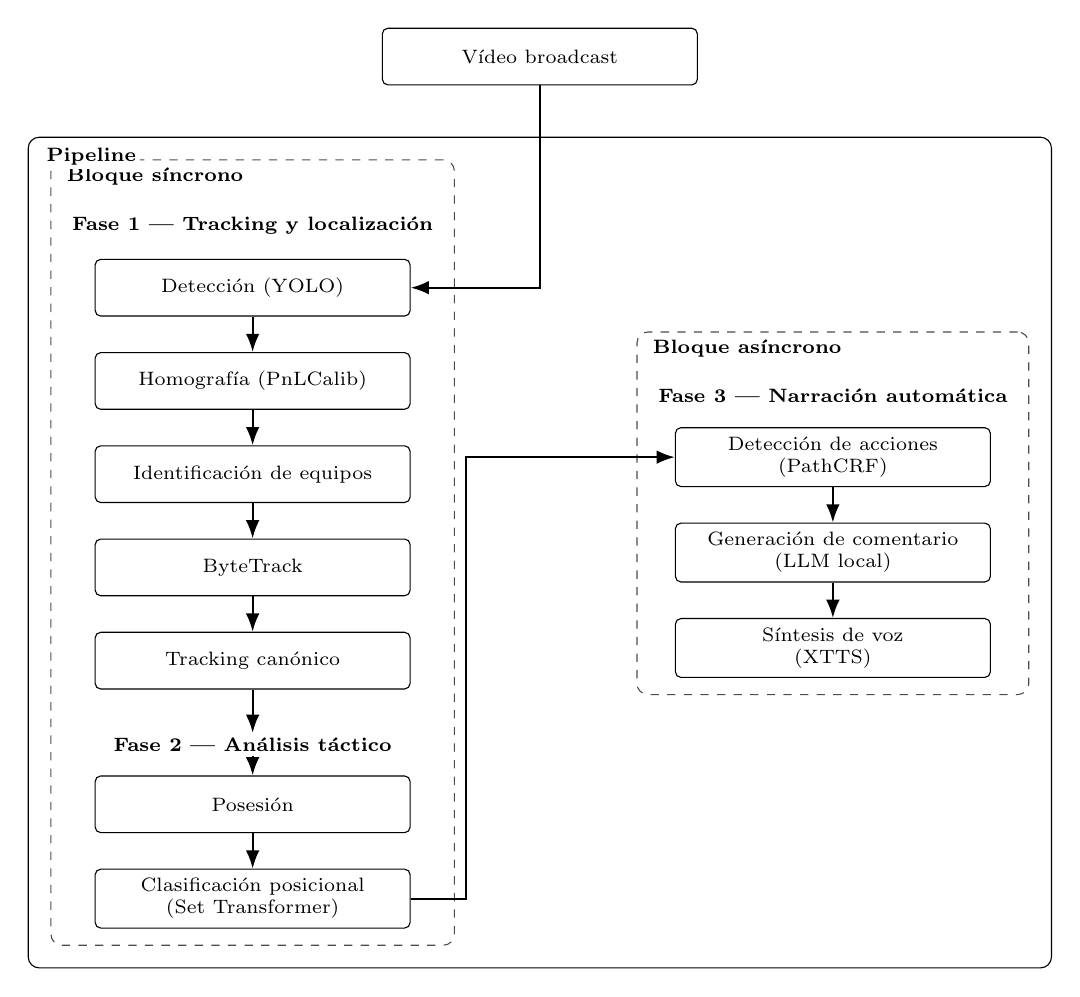
\begin{tikzpicture}[
    font=\scriptsize,
    node distance=0.45cm and 0.7cm,
    block/.style={
        rectangle,
        draw=black,
        rounded corners=2pt,
        minimum width=4.0cm,
        minimum height=0.72cm,
        align=center,
        fill=white
    },
    title/.style={
        font=\scriptsize\bfseries,
        fill=white,
        inner sep=1.5pt
    },
    container/.style={
        rectangle,
        draw=black,
        rounded corners=4pt,
        inner sep=8pt,
        fill=none
    },
    subcontainer/.style={
        rectangle,
        draw=black!70,
        dashed,
        rounded corners=4pt,
        inner sep=6pt,
        fill=none
    },
    arrow/.style={-{Latex}, thick}
]

% =========================================================
% BLOQUE SÍNCRONO: FASE 1 Y FASE 2
% =========================================================

\node[title] (fase1label) {Fase 1 --- Tracking y localización};

\node[block, below=0.25cm of fase1label] (det)
{Detección (YOLO)};

\node[block, below=of det] (hom)
{Homografía (PnLCalib)};

\node[block, below=of hom] (equipos)
{Identificación de equipos};

\node[block, below=of equipos] (byte)
{ByteTrack};

\node[block, below=of byte] (canonico)
{Tracking canónico};

\node[title, below=0.55cm of canonico] (fase2label)
{Fase 2 --- Análisis táctico};

\node[block, below=0.25cm of fase2label] (posesion)
{Posesión};

\node[block, below=of posesion] (posiciones)
{Clasificación posicional\\(Set Transformer)};

\node[inner sep=0pt, minimum size=0pt] (syncpad)
at ($(fase1label.north)+(0,0.45)$) {};

\node[subcontainer,
      fit=(syncpad)(fase1label)(det)(hom)(equipos)(byte)(canonico)
          (fase2label)(posesion)(posiciones)] (syncbox) {};

\node[title, anchor=north west]
at ($(syncbox.north west)+(0.15,-0.05)$)
{Bloque síncrono};

% =========================================================
% BLOQUE ASÍNCRONO: FASE 3
% =========================================================

\coordinate (asynccenter) at ($(syncbox.east)+(4.8cm,0)$);

\node[block] (comentario) at (asynccenter)
{Generación de comentario\\(LLM local)};

\node[block, above=of comentario] (acciones)
{Detección de acciones\\(PathCRF)};

\node[block, below=of comentario] (tts)
{Síntesis de voz\\(XTTS)};

\node[title, above=0.25cm of acciones] (fase3label)
{Fase 3 --- Narración automática};

\node[inner sep=0pt, minimum size=0pt] (asyncpad)
at ($(fase3label.north)+(0,0.45)$) {};

\node[subcontainer,
      fit=(asyncpad)(fase3label)(acciones)(comentario)(tts)] (asyncbox) {};

\node[title, anchor=north west]
at ($(asyncbox.north west)+(0.15,-0.05)$)
{Bloque asíncrono};

% =========================================================
% CONTENEDOR ÚNICO: PIPELINE
% =========================================================

\node[inner sep=0pt, minimum size=0pt] (pipepad)
at ($(syncbox.north west)!0.5!(asyncbox.north east)+(0,0.95)$) {};

\node[container, fit=(pipepad)(syncbox)(asyncbox)] (pipelinebox) {};

\node[title, anchor=north west]
at ($(pipelinebox.north west)+(0.18,-0.08)$)
{Pipeline};

% =========================================================
% NODO EXTERNO: VÍDEO BROADCAST
% =========================================================

\node[block, anchor=south] (video)
at ($(pipelinebox.north)+(0,0.65cm)$)
{Vídeo broadcast};

% =========================================================
% FLECHAS
% =========================================================

% Entrada externa hacia el pipeline:
% baja y gira una sola vez hacia la izquierda hasta entrar por det.east
\draw[arrow] (video.south) |- (det.east);

% Flujo síncrono
\draw[arrow] (det) -- (hom);
\draw[arrow] (hom) -- (equipos);
\draw[arrow] (equipos) -- (byte);
\draw[arrow] (byte) -- (canonico);

\draw[arrow] (canonico) -- (fase2label);
\draw[arrow] (fase2label) -- (posesion);
\draw[arrow] (posesion) -- (posiciones);

% Paso del bloque síncrono al bloque asíncrono
\draw[arrow] (posiciones.east) -- ++(0.7,0) |- (acciones.west);

% Flujo asíncrono
\draw[arrow] (acciones) -- (comentario);
\draw[arrow] (comentario) -- (tts);

\end{tikzpicture}
}
\caption[Arquitectura software del pipeline]{Arquitectura software del pipeline del sistema. Se organiza en un bloque síncrono, que agrupa las fases de detección, localización, tracking y análisis táctico, y un bloque asíncrono, responsable de la narración automática.}
\label{fig:arquitectura-software}
\end{figure}

\section{Organización de la Memoria}

La memoria comienza con el \hyperref[cap:tecnologiasUtilizadas]{Capítulo~\ref*{cap:tecnologiasUtilizadas}. Tecnologías Utilizadas}, donde se presentan las principales herramientas, modelos y técnicas que sirven de base al sistema. En él se introducen, entre otros, los métodos de detección, tracking, análisis geométrico, modelado posicional, detección secuencial de eventos, generación de lenguaje y síntesis de voz.

A continuación, el \hyperref[cap:trabajoRelacionado]{Capítulo~\ref*{cap:trabajoRelacionado}. Trabajo Relacionado} revisa trabajos previos en los distintos bloques del pipeline. Esta revisión permite situar el proyecto dentro del estado del arte y contextualizar las decisiones adoptadas en tareas como la detección de jugadores y balón, el tracking multiobjeto en vídeo deportivo y la detección de eventos futbolísticos.

Una vez establecido ese contexto, el \hyperref[cap:procesamientoVisual]{Capítulo~\ref*{cap:procesamientoVisual}. Procesamiento Visual} describe la primera gran fase del sistema. En este capítulo se explica cómo se transforma el vídeo broadcast en una representación estructurada del partido mediante detección de elementos del juego, calibración geométrica del campo, clasificación de equipos, una primera capa de asociación temporal basada en ByteTrack, una segunda capa de tracking canónico y, finalmente, una evaluación heurística orientada a depurar y seleccionar la configuración final del pipeline visual.

Sobre esa salida se construye el \hyperref[cap:analisisTactico]{Capítulo~\ref*{cap:analisisTactico}. Análisis Táctico}, donde se abordan tareas de mayor nivel semántico. En él se describe, en primer lugar, una inferencia heurística de la posesión del balón. Después se presenta la inferencia de posiciones futbolísticas a partir de la disposición espacial de los jugadores y de su contexto colectivo. Finalmente, se expone la clasificación de acciones relevantes del partido, como pases, controles, robos o tiros.

La siguiente etapa se presenta en el \hyperref[cap:narracion]{Capítulo~\ref*{cap:narracion}. Narración}, centrado en la generación automática de comentarios. Este capítulo resume cómo los eventos detectados se convierten en texto narrativo mediante un modelo de lenguaje y cómo ese texto pasa posteriormente a audio mediante distintos sistemas de síntesis de voz evaluados durante el proyecto.

Antes del cierre, el \hyperref[cap:integraciónSistema]{Capítulo~\ref*{cap:integraciónSistema}. Integración del Sistema y Validación Final} explica como se consume el sistema desde una interfaz web y presenta una validación global del comportamiento del sistema en condiciones finales de uso.

Finalmente, la memoria concluye con el \hyperref[cap:conclusiones]{Capítulo~\ref*{cap:conclusiones}. Conclusiones y Trabajo Futuro}, donde se sintetizan los principales resultados obtenidos, se analizan las limitaciones del sistema y se recogen posibles líneas de mejora para continuar el desarrollo del trabajo.



\chapter{Tecnologías Utilizadas}
\label{cap:tecnologiasUtilizadas}

En este capítulo se presentan las principales tecnologías, modelos y herramientas empleados en el desarrollo del sistema, explicando su funcionamiento general y el papel que desempeñan dentro del pipeline. El objetivo no es describir la implementación concreta del proyecto, sino introducir los fundamentos necesarios.

\section{Detección de objetos con YOLO}
\label{sec:yolo-tecnologias}

La detección de objetos es una de las tareas principales dentro de la visión por computador. Su objetivo es localizar e identificar las instancias de una o varias clases presentes en una imagen, normalmente mediante cajas \textit{bounding box} asociadas a una etiqueta y a una puntuación de confianza. En esta sección se describe cómo YOLO afronta este problema.

\subsection{Modelo de detección YOLO}

Uno de los enfoques más utilizados para detección en tiempo real es YOLO \citep{RedmonYOLO2016}. Esta red neuronal convolucional plantea la detección como un problema de regresión directa sobre la imagen completa, prediciendo cajas y clases en una sola pasada. Esta filosofía de detector de una etapa resulta especialmente adecuada para vídeo, donde no basta con obtener buena precisión en imágenes aisladas, sino que también es importante mantener una velocidad de inferencia suficiente para procesar secuencias largas. Las implementaciones modernas de Ultralytics \citep{UltralyticsYOLO2023} \footnote{Ultralytics es una empresa y comunidad de desarrollo de software especializada en herramientas de visión por computador, conocida principalmente por mantener implementaciones modernas de YOLO y facilitar su entrenamiento, evaluación y despliegue.} han popularizado su uso práctico mediante modelos preentrenados, herramientas de entrenamiento y despliegue, y soporte para fine-tuning sobre datasets propios.


En la formulación original de YOLO, la imagen se divide en una cuadrícula de $S \times S$ celdas. Cada celda es responsable de predecir los objetos cuyo centro cae dentro de ella. Para cada celda, la red estima una o varias cajas delimitadoras junto con una confianza de objeto y una distribución de probabilidad sobre las clases. De forma simplificada, cada predicción puede representarse como:

\[
(x, y, w, h, C)
\]

donde $x$ e $y$ indican la posición del centro de la caja, $w$ y $h$ representan su anchura y altura, y $C$ expresa la confianza asociada a la existencia de un objeto y a la calidad de la localización. Además, la red predice las probabilidades de clase. La puntuación final de una detección puede entenderse como la combinación entre la confianza de objeto y la probabilidad de clase:

\[
score = P(\text{objeto}) \cdot P(\text{clase} \mid \text{objeto})
\]

El flujo de este modelo de detección se muestra en la \hyperref[fig:yolo-grid]{Figura~\ref*{fig:yolo-grid}}. La red comparte un mismo \textit{backbone} para extraer características visuales de la imagen y, a partir de ellas, produce simultáneamente la regresión de cajas, la confianza y la clasificación. Aunque las versiones modernas de YOLO utilizadas por implementaciones como Ultralytics han evolucionado respecto al modelo original, incorporando cabezas de detección multiescala y mejores funciones de pérdida, la idea central sigue siendo la misma: obtener cajas y clases directamente en una única pasada de la red.

\begin{figure}[H]
    \centering
    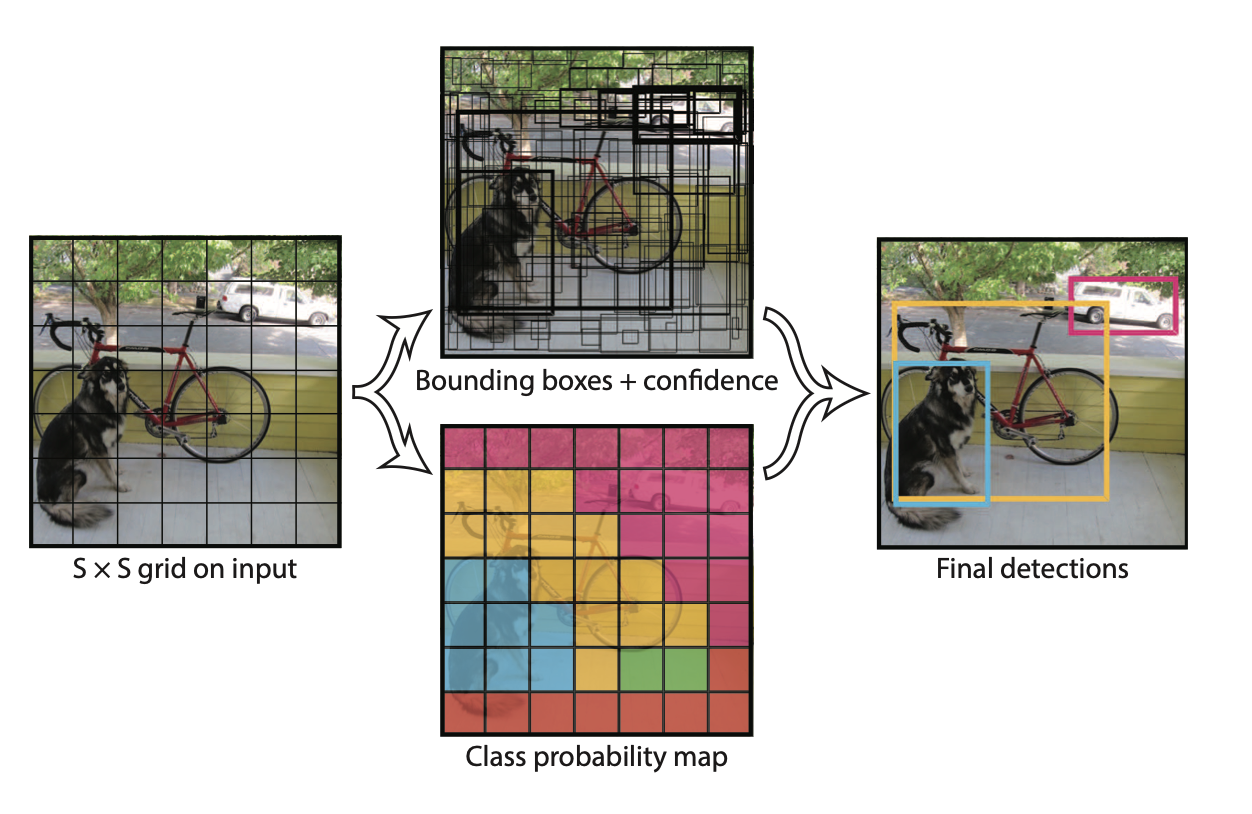
\includegraphics[width=0.9\textwidth]{Imagenes/Propias/YOLO2.png}
    \caption[Esquema conceptual de YOLO como detector de una etapa]{Esquema conceptual de YOLO como detector de una etapa: división espacial, regresión de cajas y clasificación. Fuente: reproducido de \citep{RedmonYOLO2016}.}
    \label{fig:yolo-grid}
\end{figure}

Durante el entrenamiento, la función de pérdida combina varios objetivos. Por un lado, penaliza el error de localización entre la caja predicha y la caja real. Por otro lado, penaliza los errores de confianza, diferenciando entre regiones que contienen objetos y regiones de fondo. Finalmente, incorpora el error de clasificación. Esto obliga al modelo a aprender simultáneamente tres tareas: localizar el objeto, decidir si realmente existe y asignarle una clase correcta.

\subsection{Post-procesado mediante Non-Maximum Suppression}
Tras la inferencia, es habitual que el detector produzca varias cajas muy próximas para un mismo objeto. Para eliminar estas detecciones redundantes se aplica \textit{Non-Maximum Suppression} (NMS). Este algoritmo ordena las cajas por puntuación, conserva la de mayor confianza y elimina aquellas cajas de la misma clase cuyo solape con ella supere un determinado umbral. El solape se mide mediante la intersección sobre la unión, o IoU:

\[
IoU(A,B)=\frac{\operatorname{area}(A \cap B)}{\operatorname{area}(A \cup B)}
\]

Si dos cajas tienen un IoU superior al umbral $\lambda_{nms}$, se considera que ambas representan el mismo objeto y se conserva únicamente la de mayor confianza. La \hyperref[fig:yolo-nms]{Figura~\ref*{fig:yolo-nms}} ilustra este proceso, en el que múltiples predicciones cercanas se reducen a una única caja final. Esto también puede observarse en el segundo paso de la \hyperref[fig:yolo-grid]{Figura~\ref*{fig:yolo-grid}}.

\begin{figure}[H]
    \centering
    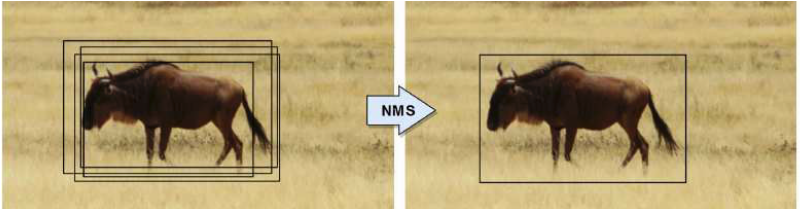
\includegraphics[width=0.9\textwidth]{Imagenes/Propias/YOLO1.png}
    \caption[Postproceso mediante Non-Maximum Suppression]{Postproceso mediante Non-Maximum Suppression para eliminar cajas redundantes.
    Fuente: reproducido de \citep{BesadaAnalisisSenal2025}}
    \label{fig:yolo-nms}
\end{figure}


\subsection{Métricas de evaluación en detección de objetos}
\label{subsec:metricas-deteccion-objetos}

Para evaluar un detector de objetos no basta con comprobar si predice la clase correcta, sino que también es necesario analizar la calidad de la localización espacial. Para ello se utiliza habitualmente la IoU. Una detección se considera correcta si su IoU supera un determinado umbral y la clase predicha coincide con la clase real.

A partir de esta correspondencia entre predicciones y anotaciones reales se calculan métricas como la precisión y el recall. La precisión mide qué proporción de las detecciones realizadas por el modelo son correctas, mientras que el recall mide qué proporción de los objetos reales han sido detectados. Estas métricas se definen como:

\[
\text{Precisión} = \frac{TP}{TP + FP}
\]

\[
\text{Recall} = \frac{TP}{TP + FN}
\]

donde $TP$ representa el número de verdaderos positivos, $FP$ el número de falsos positivos y $FN$ el número de falsos negativos. En el contexto de la detección de objetos, un verdadero positivo corresponde a una predicción cuya clase es correcta y cuya IoU con la caja real supera el umbral establecido. Un falso positivo es una detección incorrecta o duplicada, mientras que un falso negativo corresponde a un objeto real que no ha sido detectado.

El valor F1 combina ambas métricas mediante su media armónica:

\[
F1 = 2 \cdot \frac{\text{Precisión} \cdot \text{Recall}}{\text{Precisión} + \text{Recall}}
\]

Esta métrica resulta útil cuando se desea valorar conjuntamente falsos positivos, asociados a la precisión, y falsos negativos, asociados al recall.

En detección de objetos también es habitual emplear la métrica mAP (\textit{mean Average Precision}). El mAP@50 considera correcta una detección cuando alcanza un IoU mínimo de 0.50, mientras que el mAP@50-95 calcula el rendimiento medio usando varios umbrales de IoU entre 0.50 y 0.95.


\subsection{Papel de YOLO dentro del pipeline}
En este proyecto, YOLO se utiliza como detector inicial del pipeline para localizar jugadores, árbitros, porteros y balón en cada fotograma. Sus salidas sirven como entrada para las etapas posteriores de seguimiento y análisis temporal.

En esta sección se ha introducido YOLO desde un punto de vista conceptual. Su aplicación concreta dentro del sistema se desarrolla posteriormente en la \hyperref[sec:deteccion-elementos-juego]{Sección~\ref*{sec:deteccion-elementos-juego}, Detección de elementos del juego}.

% \section{Analisis de color mediante CIE LAB y KMeans}
\subsection{Espacios de color y color dominante}
El análisis de color es una técnica utilizada en visión por computador para describir, comparar y agrupar regiones de una imagen a partir de su apariencia cromática. Este tipo de información puede resultar útil cuando se desea distinguir elementos visualmente similares en forma o tamaño, pero diferenciados por su color dominante.

Desde el punto de vista clásico, una estrategia sencilla y eficiente consiste en extraer el color dominante de una región de interés obtenida a partir de una detección. El uso directo del espacio RGB puede ser problemático, porque mezcla información cromática y luminancia, de modo que cambios de iluminación, sombras o balance de blancos alteran de forma significativa las distancias entre colores. Por ello, resulta habitual transformar la imagen a espacios más adecuados para comparación perceptual, como CIE L*a*b*, donde el canal L* representa la luminosidad y los canales a* y b* codifican los ejes cromáticos \citep{cie1976lab}. Esta separación permite que las diferencias de color sean más estables que en RGB cuando varían las condiciones de captura.

Sobre este espacio de color puede aplicarse \textit{k-means}, un algoritmo de agrupamiento no supervisado que divide un conjunto de muestras en $K$ grupos minimizando la suma de distancias cuadráticas a sus centroides \citep{macqueen1967kmeans,lloyd1982least}:

\[
\min_{\mu_1,\dots,\mu_K} \sum_{i=1}^{n} \min_{k \in \{1,\dots,K\}} \|x_i - \mu_k\|_2^2
\]

Aplicado al análisis de imagen, cada muestra puede corresponder a un píxel o a una representación cromática extraída de una región. El resultado del agrupamiento permite identificar colores dominantes y separar componentes visuales con apariencia distinta. Esta técnica tiene la ventaja de no requerir entrenamiento supervisado y de poder adaptarse a cada imagen o secuencia de entrada. Sin embargo, su rendimiento puede verse afectado cuando los colores son muy parecidos, cuando la región analizada contiene demasiado fondo o cuando existen cambios fuertes de iluminación.

\subsection{Papel del análisis de color dentro del pipeline}
En el contexto de este proyecto, el análisis de color se utiliza para apoyar la identificación automática de equipos a partir del color de camiseta de los jugadores. Una vez detectado un jugador, el recorte asociado a su \textit{bounding box} contiene información visual que puede emplearse para estimar el color dominante de la camiseta y compararlo con el de otros jugadores.

Esta idea puede aplicarse en dos niveles. En primer lugar, dentro del recorte de cada jugador, para separar la camiseta de otros píxeles pertenecientes al fondo, al césped, a la piel o al pantalón. En segundo lugar, sobre los colores dominantes estimados para varios jugadores, para agruparlos en los dos equipos principales. De esta forma, la información cromática se convierte en una señal adicional que puede utilizarse en etapas posteriores del sistema, especialmente en el tracking multiobjeto y en la generación de una representación estructurada del partido.

Frente a un clasificador supervisado de camisetas, esta solución tiene la ventaja de no requerir un conjunto de entrenamiento específico para cada partido y de poder adaptarse al inicio de cada vídeo. Su principal limitación aparece cuando ambos equipos usan colores parecidos, cuando el recorte incluye demasiado fondo o cuando la cámara introduce cambios fuertes de exposición.
\section{Calibración geométrica mediante homogarfía}
\label{sec:homografia-tecnologias}
En muchos problemas de visión por computador, las coordenadas observadas en una imagen no representan directamente la posición real de los objetos en la escena. La perspectiva, el zoom, la posición de la cámara y los movimientos de la misma pueden hacer que dos puntos separados por la misma distancia física aparezcan a distancias muy distintas en píxeles. Por este motivo, cuando se desea razonar sobre posiciones reales, resulta necesario calibrar la cámara y transformar puntos desde el plano de la imagen hacia un plano de referencia.

\subsection{Homografía entre planos}

Cuando la superficie observada puede aproximarse como un plano, la relación entre los puntos de la imagen y los puntos de dicho plano puede modelarse mediante una homografía. Una homografía es una transformación proyectiva \footnote{Una transformación proyectiva es una operación geométrica que mapea puntos de un plano (o espacio) a otro, preservando las líneas rectas pero no necesariamente el paralelismo, ángulos o distancias} entre dos planos, representada mediante una matriz $H \in \mathbb{R}^{3 \times 3}$. En este contexto, permite relacionar coordenadas en píxeles de la imagen broadcast con coordenadas sobre una representación 2D del terreno de juego.

Para expresar esta transformación se utilizan coordenadas homogéneas. Este tipo de representación consiste en añadir a un punto bidimensional como $(u,v)$, una tercera componente y se escribe como $(u,v,1)$. Esta representación permite describir transformaciones de perspectiva mediante una multiplicación matricial. Así, un punto de imagen $(u,v)$ y su correspondiente punto del plano de referencia $(x,y)$ se relacionan mediante:

\[
\begin{bmatrix}
x \\
y \\
1
\end{bmatrix}
\sim
H
\begin{bmatrix}
u \\
v \\
1
\end{bmatrix}
\]

Tras aplicar la matriz, las coordenadas resultantes se normalizan dividiendo por la tercera componente para volver a obtener coordenadas bidimensionales.

La \hyperref[fig:exp-homografia]{Figura~\ref*{fig:exp-homografia}} muestra una interpretación geométrica de esta idea, en la que los puntos de un plano se proyectan sobre otro plano, estableciendo una correspondencia entre ambas superficies.

\begin{figure}[H]
    \centering
    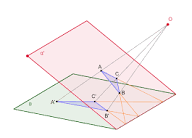
\includegraphics[width=0.3\textwidth]{Imagenes/Propias/exp_homografia.png}
    \caption[Esquema de homografía entre planos]{
Esquema geométrico de una homografía entre dos planos proyectivos. Los puntos del plano original se proyectan desde un centro de proyección sobre un segundo plano, estableciendo una correspondencia entre ambas superficies. Fuente: reproducida de \citep{DibujoSecundariaTransformaciones}.
}
    \label{fig:exp-homografia}
\end{figure}

Esta transformación no conserva necesariamente distancias, ángulos ni áreas, pero sí permite transformar puntos entre dos planos cuando existen suficientes correspondencias geométricas. Estas correspondencias pueden obtenerse a partir de elementos conocidos de la escena. Si se identifican suficientes referencias, es posible estimar la homogradia que alinea la imagen con una representación métrica del plano observado.

\subsection{Estimación de homografía mediante PnLCalib}
PnLCalib \citep{GutierrezPnLCalib2024} es un método de calibración de cámaras en vídeo deportivo diseñado para obetener una transformación geométrica que permita proyectar la imagen broadcast sobre un modelo geométrico del campo de fútbol. A diferencia de otros enfoques que dependen únicamente de puntos característicos o de una búsqueda sobre posibles poses de cámara, PnLCalib combina información de puntos y líneas del terreno de juego para obtener una estimación más robusta.

El método parte de una idea sencilla: el campo de fútbol tiene una geometría conocida. Líneas de banda, áreas, círculo central, puntos de penalti e intersecciones entre marcas del terreno pueden utilizarse como referencias para estimar la relación entre la imagen y el modelo del campo. Para ello, PnLCalib emplea redes encoder-decoder que predicen mapas de calor de \textit{keypoints} y extremos de líneas visibles en el frame. A partir de estas predicciones se extraen correspondencias entre la imagen y el modelo geométrico del campo.

El proceso general de PnLCalib se resume en la \hyperref[fig:pnlcalib-pipeline]{Figura~\ref*{fig:pnlcalib-pipeline}} y se divide en dos etapas principales: la generación de datos de entrenamiento y la fase de inferencia.

En la primera etapa, el método parte de las anotaciones de SoccerNet y de la geometría conocida del campo de fútbol para construir las referencias que aprenderán las redes. El resultado de esta etapa no es un nuevo conjunto de imágenes, sino un conjunto de pares de entrenamiento en los que cada frame queda asociado a 57 mapas de calor que indican la posición esperada de 57 puntos característicos del terreno de juego y a 23 mapas de calor de las líneas del campo.

Durante la fase de inferencia, PnLCalib recibe un frame de entrada y utiliza dos redes encoder-decoder. La primera red predice $57+1$ mapas de calor: un canal para cada \textit{keypoint} predefinido y un canal adicional de fondo. Cada mapa de calor indica la probabilidad de que el punto correspondiente se encuentre en cada posición de la imagen, por lo que la localización final del punto se obtiene seleccionando las zonas de mayor activación. La segunda red predice $23+1$ mapas de calor asociados a las líneas del campo: un canal por cada línea considerada y un canal adicional de borde. En este caso, cada canal contiene dos activaciones principales, correspondientes a los extremos visibles de la línea.

A partir de los máximos de estos mapas de calor se extraen las posiciones en la imagen de los puntos característicos y de los extremos de las líneas en la imagen. Además, las líneas detectadas pueden utilizarse para recuperar puntos no observados directamente mediante intersecciones entre líneas, aumentando así el número de referencias disponibles. Además las posiciones en el modelo del campo de todas esas referencias son conocidas, por tanto, con estas correspondencias entre la imagen y el modelo geométrico del campo se calcula una calibración inicial mediante métodos geométricos.

Finalmente, PnLCalib incorpora un módulo de refinamiento PnL, de \textit{Points and Lines}, que ajusta la calibración inicial utilizando conjuntamente la información de puntos y líneas. Este refinamiento se plantea como un problema de optimización no lineal orientado a reducir el error de reproyección, es decir, la diferencia entre las referencias observadas en la imagen y las referencias proyectadas desde el modelo geométrico del campo.

\begin{figure}[H]
    \centering
    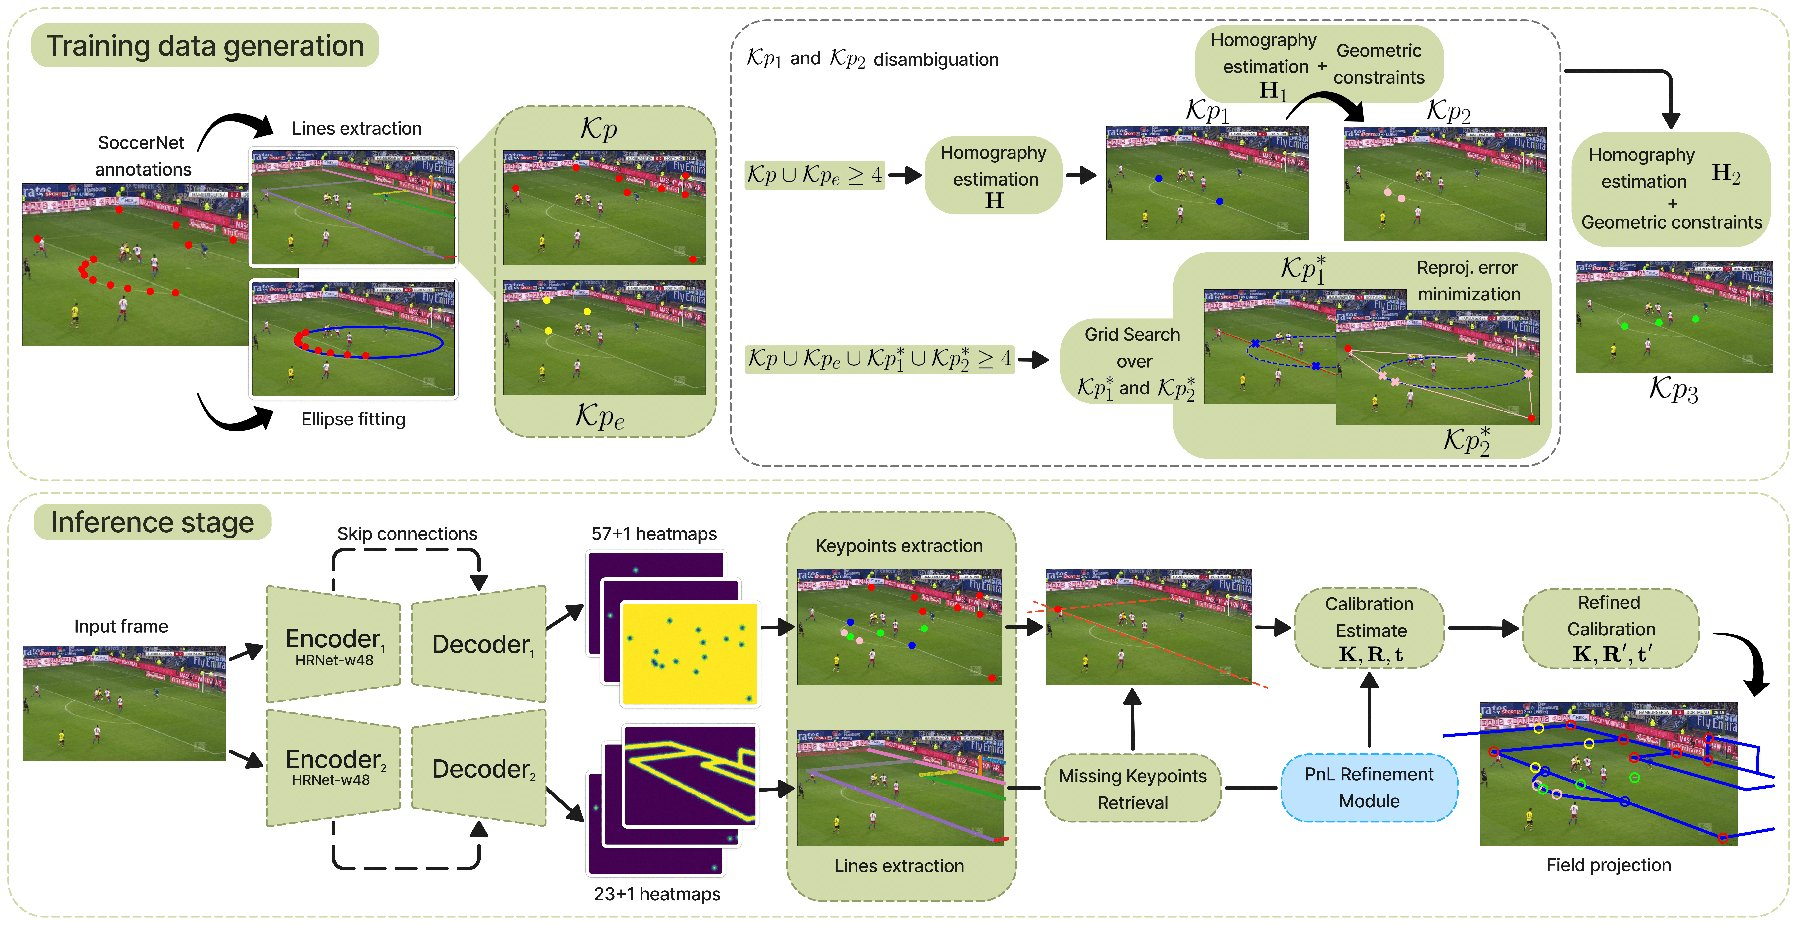
\includegraphics[width=0.9\textwidth]{Imagenes/Propias/pipeline.jpg}
    \caption[Pipeline de PnLCalib]{
    Pipeline de PnLCalib para estimar la calibración del campo mediante \textit{keypoints}, líneas y refinamiento geométrico. Fuente: reproducida de \citep{GutierrezPnLCalib2024}.
    }
    \label{fig:pnlcalib-pipeline}
\end{figure}

La \hyperref[fig:field-reconstruction]{Figura~\ref*{fig:field-reconstruction}} muestra un ejemplo visual de este proceso. Las líneas proyectadas representan la estructura geométrica estimada del campo sobre la imagen original, mientras que los puntos coloreados indican referencias detectadas o utilizadas durante el ajuste. Este tipo de visualización permite comprobar de forma intuitiva si la calibración obtenida es coherente con la escena observada.

\begin{figure}[H]
    \centering
    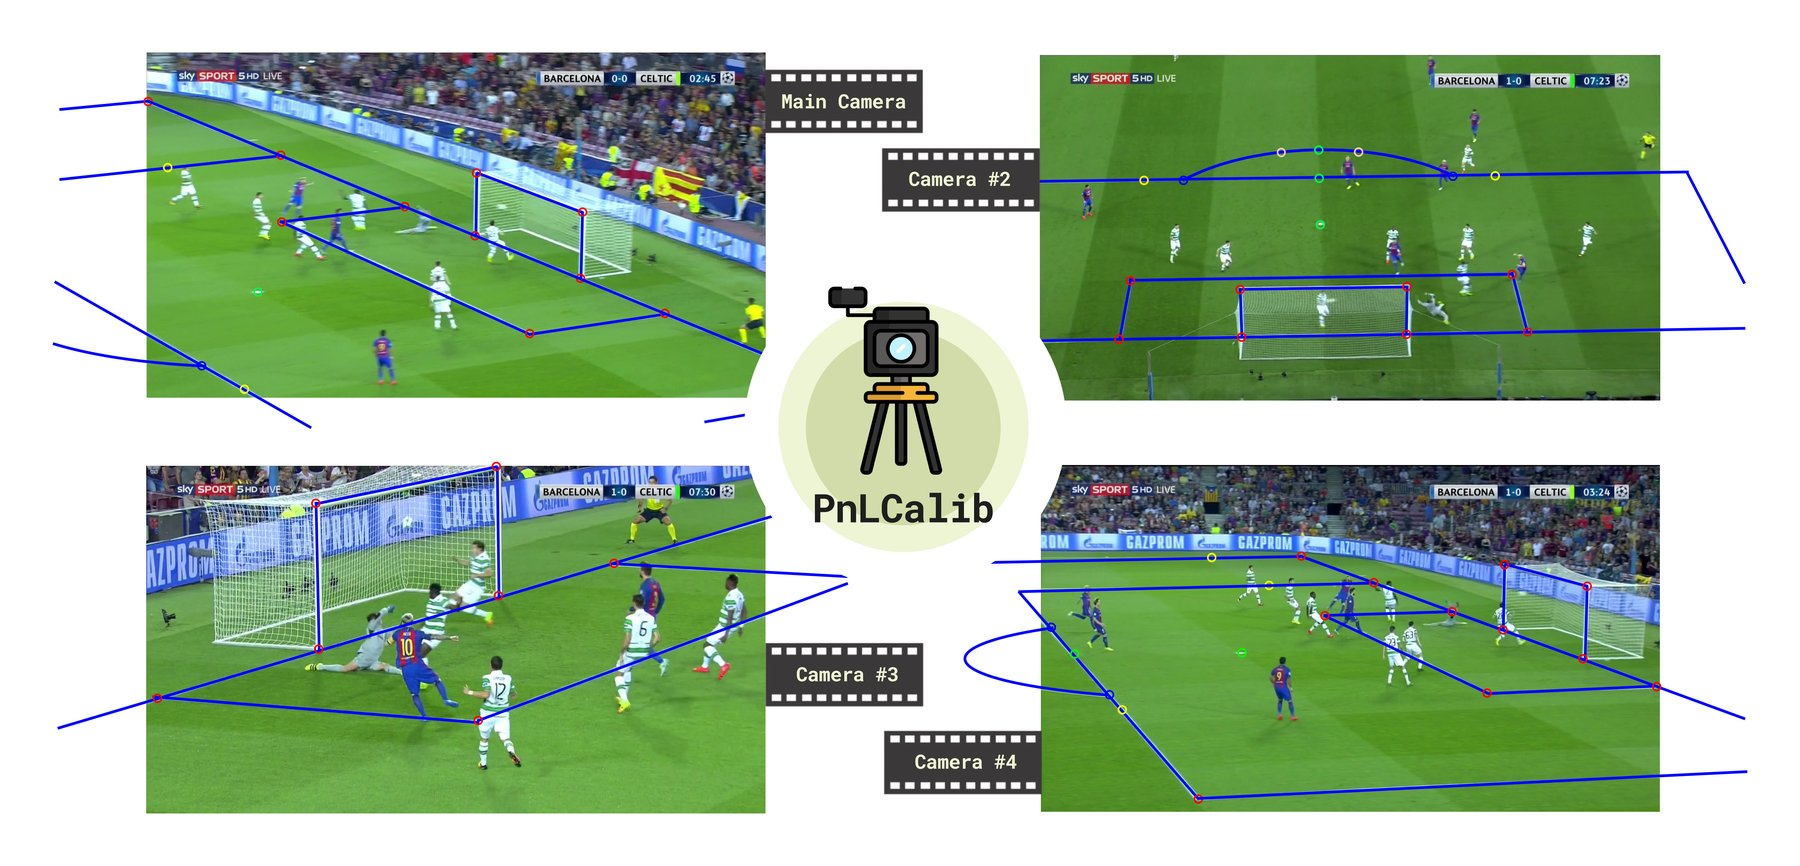
\includegraphics[width=0.95\textwidth]{Imagenes/Propias/field_reconstruction.jpg}
    \caption[Reconstrucción geométrica sobre imágenes broadcast]{
    Reconstrucción geométrica sobre imágenes broadcast mediante líneas y puntos de referencia. Fuente: reproducida de \citep{PnLCalibRepo2024}.
    }
    \label{fig:field-reconstruction}
\end{figure}

\subsection{Papel de la homografía dentro del pipeline}
En el contexto de este proyecto, la homografía permite transformar las detecciones obtenidas en la imagen broadcast hacia una representación 2D del terreno de juego. De esta forma, las detecciones obtenidas en píxeles pueden expresarse en un sistema de coordenadas más próximo al espacio físico real del partido.

Una vez estimada la homografía, cada detección puede proyectarse al campo a partir de un punto representativo. En el caso de los jugadores, se utiliza habitualmente el punto inferior central de la \textit{bounding box}, ya que aproxima la posición de contacto del jugador con el plano del suelo.

La principal ventaja de trabajar en coordenadas del campo es que las distancias pasan a tener una interpretación física. Esto resulta útil para etapas posteriores del pipeline, como el tracking multiobjeto, la clasificación posicional o el análisis de eventos. Por ejemplo, una identidad perdida puede recuperarse si reaparece en una posición compatible sobre el terreno de juego.

No obstante, la calibración también introduce riesgos. Si la homografía estimada es incorrecta, todas las posiciones proyectadas quedarán desplazadas de forma sistemática. En vídeo broadcast, este problema puede aparecer cuando la cámara cambia bruscamente, cuando se observa una zona reducida del campo o cuando las líneas visibles son insuficientes. Por este motivo, la homografía debe tratarse como una señal valiosa, pero no infalible, y conviene que el pipeline pueda continuar aunque algunos frames no dispongan de una proyección fiable.

La integración concreta de la calibración en el sistema desarrollado, incluyendo las estrategias de robustez y los criterios prácticos de aceptación de homografías, se describe posteriormente en la 
\hyperref[sec:calibracion-campo-proyeccion-metricas]{Sección~\ref*{sec:calibracion-campo-proyeccion-metricas}}

\section{Tracking multiobjeto}
\label{sec:tracking-tecnologias}

El tracking multiobjeto consiste en mantener la identidad de múltiples objetos a lo largo de una secuencia de vídeo. A diferencia de la detección de objetos, que produce resultados independientes en cada frame, el tracking introduce una asociación temporal entre detecciones consecutivas. Su objetivo es asignar un identificador persistente a cada objeto, de forma que pueda reconstruirse su trayectoria a lo largo del tiempo.

Este problema suele abordarse combinando detección, predicción de movimiento y asociación de detecciones. En cada frame, el detector proporciona un conjunto de cajas candidatas. A continuación, el tracker compara estas detecciones con las trayectorias activas y decide qué detección corresponde a cada identidad previa, qué objetos han desaparecido temporalmente y qué detecciones deben iniciar nuevas trayectorias. Esta asociación puede basarse en medidas geométricas, como el solape entre cajas, la distancia entre posiciones o la coherencia del movimiento estimado.

\subsection{ByteTrack}
ByteTrack \citep{ZhangByteTrack2022} es una de las referencias recientes más relevantes en tracking multiobjeto. Su principal aportación consiste en no descartar directamente las detecciones con baja confianza, ya que algunas de ellas pueden corresponder a objetos reales parcialmente ocluidos, lejanos o difíciles de detectar. En lugar de ello, ByteTrack utiliza estas detecciones en una segunda etapa de asociación, lo que permite recuperar trayectorias que otros métodos podrían fragmentar.

El funcionamiento de ByteTrack puede entenderse como un ciclo que se repite en cada frame. En primer lugar, el detector proporciona un conjunto de cajas con sus puntuaciones de confianza. Estas detecciones se separan en dos grupos mediante umbrales: detecciones de alta confianza, que se consideran más fiables, y detecciones de baja confianza, que no son suficientes para iniciar nuevas trayectorias pero sí pueden servir para actualizar trayectorias ya existentes.

Antes de realizar la asociación, las trayectorias activas se predicen hacia el frame actual mediante un filtro de Kalman \citep{Kalman1960}. Este filtro estima la posición esperada de cada objeto a partir de su estado anterior, habitualmente representado mediante la posición y tamaño de la caja. De esta forma, el tracker no compara las nuevas detecciones con la última posición observada sin más, sino con una predicción de dónde debería encontrarse cada objeto en el frame actual.

La asociación se realiza en varias fases. En la primera fase, ByteTrack compara las trayectorias activas y perdidas recientemente con las detecciones de alta confianza. Para ello calcula una matriz de costes basada normalmente en la IoU entre cajas, de modo que una detección se asocia a una trayectoria si su solape con la predicción del track es suficientemente alto. Las asociaciones válidas actualizan el estado del track y mantienen su identidad.

Después, las trayectorias que no han podido asociarse en la primera fase se comparan con las detecciones de baja confianza. Esta segunda asociación es la característica distintiva de ByteTrack. Una detección de baja confianza no se utiliza para crear un nuevo objeto, ya que podría ser ruido o fondo, pero sí puede ser útil para mantener una trayectoria ya existente cuando el detector ha reducido temporalmente su seguridad. De este modo, un jugador parcialmente oculto o detectado con baja confianza puede seguir asociado a su identidad previa.

Además de los tracks activos, ByteTrack mantiene otros estados internos. Los tracks no confirmados corresponden normalmente a trayectorias recién creadas que todavía no han sido observadas durante suficientes frames (si no se asocian de nuevo rápidamente, se eliminan). Los tracks perdidos son identidades que no han encontrado una detección compatible en el frame actual, pero que se conservan durante un número limitado de frames por si el objeto reaparece. Si un track permanece perdido durante más tiempo del permitido por el parámetro de memoria del tracker, se marca como eliminado. Finalmente, las detecciones de alta confianza que no han sido asociadas a ningún track existente pueden iniciar nuevas trayectorias si superan un umbral mínimo de confianza.

La \hyperref[fig:bytetrack-esquema]{Figura~\ref*{fig:bytetrack-esquema}} resume este proceso. Primero se realiza la asociación con detecciones de alta confianza. Después, las trayectorias no asociadas se comparan con detecciones de baja confianza. Luego, las trayectorias no confirmadas se comparan con detecciones de alta confianza. Por último, se actualizan los estados de las trayectorias, se crean nuevos tracks cuando procede y se eliminan aquellos que han permanecido perdidos durante demasiado tiempo.

\begin{figure}[H]
    \centering
    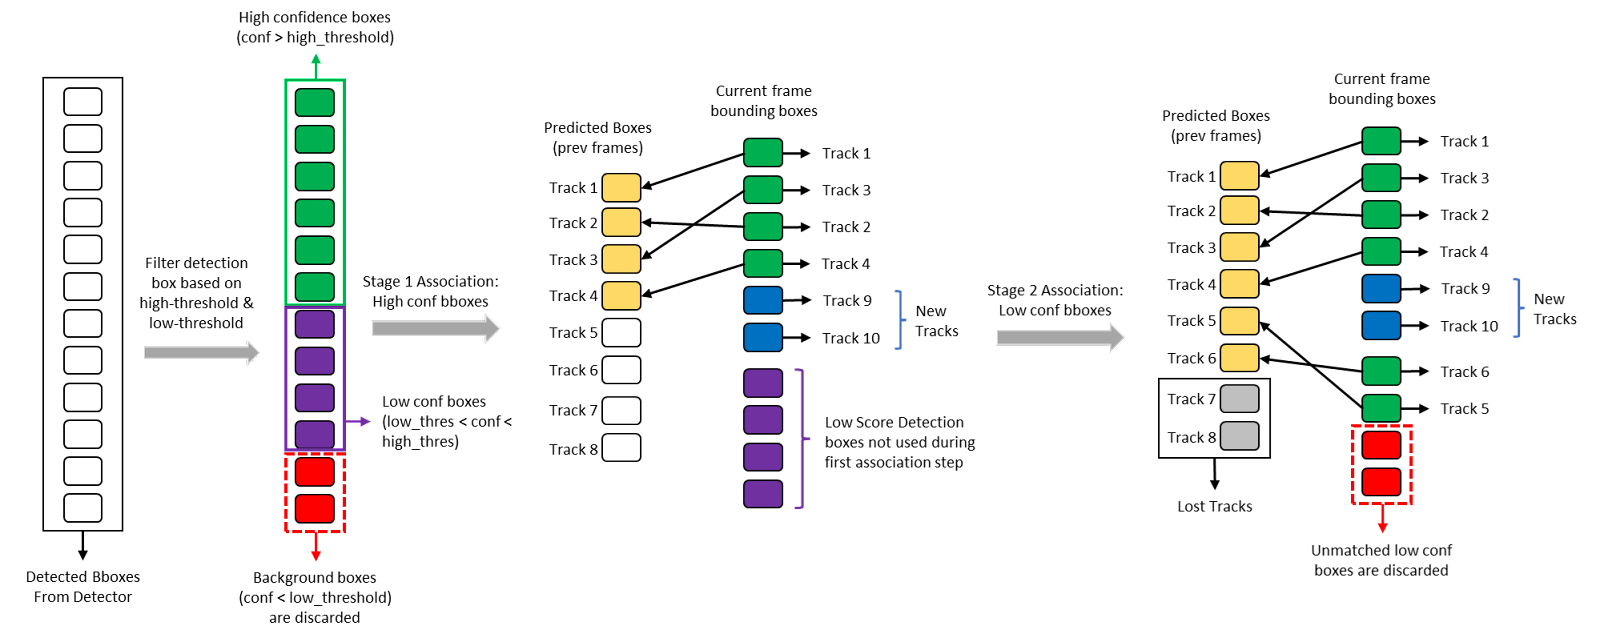
\includegraphics[width=0.9\textwidth]{Imagenes/Propias/ByteTrack.png}
    \caption[Esquema general de ByteTrack]{Esquema general de ByteTrack. El método separa las detecciones en cajas de alta y baja confianza y realiza la asociación en dos etapas, permitiendo recuperar objetos que un tracker convencional descartaría prematuramente. Fuente: reproducido de So \citep{SoByteTrack2025}.}
    \label{fig:bytetrack-esquema}
\end{figure}

Esta estrategia resulta especialmente útil en secuencias con oclusiones, movimiento rápido, cambios de escala o detecciones intermitentes. Además, ByteTrack mantiene una arquitectura relativamente simple y eficiente, ya que basa la asociación principalmente en predicción de movimiento, solape espacial y confianza de detección, sin depender necesariamente de descriptores complejos de apariencia. Esto facilita su integración en sistemas donde la latencia y la estabilidad temporal son factores importantes.

\subsection{Papel del tracking dentro del pipeline}

En este proyecto, el tracking multiobjeto permite transformar las detecciones independientes de cada frame en trayectorias persistentes de jugadores, árbitros, porteros y balón. Esta continuidad temporal es necesaria para analizar la evolución del juego y para que módulos posteriores, como la clasificación posicional o la detección de eventos puedan trabajar sobre identidades estables y analizar su evolución temporal.

El vídeo broadcast de fútbol plantea dificultades específicas para esta tarea: oclusiones frecuentes, cruces entre jugadores, similitud visual entre miembros del mismo equipo, cambios de escala, movimientos de cámara y detecciones intermitentes. Por ello, ByteTrack se utiliza como base del sistema, pero se adapta al dominio futbolístico incorporando señales adicionales y restricciones sobre las asociaciones posibles.

En nuestro caso, ByteTrack se utiliza como punto de partida, pero se realiza una profunda adaptación a nuestro caso de uso. El objetivo es aprovechar la estructura eficiente de ByteTrack, incorporando al mismo tiempo información específica del fútbol. Por tanto, el criterio de asociación no se basa únicamente en la IoU entre cajas, sino que también considera la clase detectada, el equipo estimado, la distancia entre centros de las cajas y, cuando está disponible, la posición proyectada sobre el terreno de juego. Además, se introducen restricciones duras para evitar asociaciones incompatibles y fases adicionales de asociación para recuperar correspondencias cuando el solape entre cajas no resulta suficiente.

Estas adaptaciones buscan reducir cambios de identidad, trayectorias fragmentadas y asociaciones incoherentes, problemas especialmente relevantes en un entorno como el fútbol. La implementación concreta de la capa de asociación basada en ByteTrack dentro del pipeline se describe posteriormente en la \hyperref[sec:bytetrack-layer]{Sección~\ref*{sec:bytetrack-layer}}.
\section{Modelado de conjuntos con Set Transformer}
\label{sec:setTransformer}

En esta sección se introducen los modelos Set Transformer, una arquitectura diseñada para procesar conjuntos de elementos sin imponer un orden sobre ellos. Este tipo de modelo resulta útil cuando la predicción depende tanto de las características individuales de cada elemento como de las relaciones entre todos los elementos del conjunto.

\subsection{Representación de datos como conjuntos}
En muchos problemas de aprendizaje automático, los datos de entrada no tienen una estructura secuencial natural, sino que aparecen como un conjunto de elementos. En estos casos, el orden en el que se presentan los elementos al modelo no debería modificar la salida. Por ejemplo, si un modelo recibe un conjunto de vectores que describen distintos objetos de una escena, permutar el orden de esos vectores no debería cambiar la interpretación global de la escena. 

Los modelos clásicos basados en redes densas no incorporan esta propiedad de forma directa, ya que suelen asumir que cada posición de la entrada tiene un significado fijo. Una alternativa consiste en procesar cada elemento de forma independiente y después aplicar una operación agregadora, como suma, media o máximo. Sin embargo, este tipo de aproximaciones puede ser limitado cuando la predicción depende de las relaciones entre los elementos del conjunto. Para capturar estas dependencias, las arquitecturas Set Transformer \citep{lee2019settransformer} proponen utilizar mecanismos de atención adaptados al procesamiento de conjuntos.

\subsection{Atención multi-cabeza en conjuntos}
Set Transformer se basa en el mecanismo de atención multi-cabeza introducido por los Transformers \citep{vaswani2017attention}, pero adaptado al procesamiento de conjuntos. En un Transformer aplicado a secuencias, como una frase, la atención por sí sola no conoce el orden de los elementos. Por ello, se suma una codificación posicional al vector que representa cada elemento de la entrada, permitiendo que el modelo incorpore información sobre su posición en la secuencia.

En cambio, en Set Transformer no se introduce una codificación posicional dependiente del orden de entrada, ya que los elementos del conjunto no tienen una posición secuencial con significado propio. Por ello, si se permuta el orden de los elementos de entrada, el modelo mantiene una respuesta coherente con esa permutación.

El modelo recibe un conjunto de vectores:

\[
X = \{x_1, x_2, \dots, x_n\}
\]

donde cada elemento $x_i$ representa una entidad mediante un vector de características. La atención permite que cada elemento del conjunto compare su representación con la del resto de elementos y actualice su propia codificación en función del contexto global. De esta forma, el modelo puede aprender relaciones entre elementos sin imponer un orden artificial sobre la entrada.

El bloque básico de estas arquitecturas es el mecanismo de atención. Este parte de tres representaciones: consultas $Q$, claves $K$ y valores $V$. De forma intuitiva, las consultas indican qué información busca cada elemento, las claves describen qué información ofrece cada elemento para ser comparado, y los valores contienen la información que cada elemento aporta en la combinación final que construye la salida. En la atención escalada, la similitud entre consultas y claves se calcula mediante productos escalares y se divide por $\sqrt{d}$, donde $d$ es la dimensión de las claves:

\[
\operatorname{Attention}(Q,K,V) =
\operatorname{softmax}\left(\frac{QK^T}{\sqrt{d_k}}\right)V
\]

El término $QK^T$ mide la compatibilidad entre cada consulta y cada clave. $d_k$ representa la dimensión de los vectores de clave, por tanto, la división por $\sqrt{d_k}$ es una manera de normalizar y  evitar que estos productos escalares crezcan demasiado cuando la dimensión de las claves es grande, lo que podría hacer que la función \textit{softmax} produzca distribuciones excesivamente concentradas. Por eso se denomina atención escalada.

La función \textit{softmax} convierte esas compatibilidades en pesos de atención. Cada salida se obtiene entonces como una combinación ponderada de los valores $V$: los elementos cuyas claves son más similares a una consulta reciben mayor peso en la combinación final. Por tanto, la similitud se calcula entre consultas y claves, mientras que los valores son la información que se agrega.

En la atención multi-cabeza, este cálculo no se realiza una sola vez, sino varias veces en paralelo. Cada cabeza utiliza matrices aprendidas diferentes para generar sus propias consultas, claves y valores a partir de las representaciones de entrada. Esto permite que diferentes cabezas atiendan a distintos tipos de relaciones entre elementos. Por ejemplo, en un conjunto de jugadores, una cabeza podría aprender relaciones de proximidad espacial, mientras que otra podría capturar patrones asociados a la estructura colectiva del equipo.

\subsection{Bloques principales de Set Transformer}

Dentro de Set Transformer uno de los módulos principales es el \textit{Set Attention Block} (SAB), que aplica autoatención sobre todos los elementos del conjunto. De esta forma, cada elemento puede actualizar su representación teniendo en cuenta la información del resto de elementos. El resultado no cambia frente a permutaciones: si se cambia el orden de los elementos de entrada lo único que ocurre es que las salidas se reordenan de la misma manera.

Una limitación del SAB es su coste cuadrático respecto al número de elementos, ya que cada elemento atiende directamente a todos los demás. Si el conjunto contiene $n$ elementos, esto da lugar a un coste del orden de $n \times n$.

Para reducir este coste, Set Transformer introduce el \textit{Induced Set Attention Block} (ISAB). Este bloque utiliza $m$ vectores aprendibles, llamados puntos inducidos, que actúan como una representación intermedia del conjunto, con $m \ll n$. En lugar de comparar directamente todos los elementos entre sí, los puntos inducidos resumen la información global del conjunto y los elementos atienden a esa representación resumida. Así, el coste pasa de un esquema del orden de $n \times n$ a uno del orden de $n \times m$, permitiendo capturar relaciones globales con menor coste computacional.

Cuando la tarea requiere obtener una representación global del conjunto, Set Transformer utiliza \textit{Pooling by Multihead Attention} (PMA). Este módulo emplea vectores semilla aprendibles que atienden sobre los elementos del conjunto para extraer una o varias representaciones globales. A diferencia de agregaciones simples como la media o el máximo, PMA aprende qué elementos son más relevantes para construir la salida final.

En conjunto, la arquitectura puede entenderse como una combinación de bloques de codificación y agregación. Los bloques SAB o ISAB enriquecen la representación de cada elemento a partir de sus relaciones con el resto del conjunto, mientras que PMA produce una representación global adecuada para tareas de clasificación o predicción a nivel de conjunto.

\subsection{Papel de Set Transformer dentro del pipeline}
En este proyecto, Set Transformer se utiliza para la clasificación posicional de los jugadores. Esta tarea se plantea como un problema contextual, ya que el rol de un jugador no depende únicamente de sus coordenadas instantáneas, sino también de su relación espacial con el resto del equipo. Un lateral, un central o un mediocentro pueden ocupar zonas similares en determinados momentos del partido, por lo que es necesario considerar la estructura colectiva para realizar una predicción más coherente.

Esta tarea encaja con el modelado de conjuntos, ya que los jugadores de un mismo equipo no forman una secuencia con un orden natural, sino un conjunto de elementos relacionados. Cada jugador se representa mediante un vector de características propias, como posición normalizada, velocidad estimada, visibilidad o distancia a determinadas zonas del campo. Además, mediante atención, el modelo puede comparar cada jugador con sus compañeros y capturar relaciones espaciales relevantes, como amplitud, profundidad o cercanía a otras posiciones.

Además, la orientación del equipo introduce una dificultad adicional: conceptos como izquierda, derecha, ataque o defensa dependen de la dirección de juego. Por ello, antes de aplicar el modelo, las coordenadas pueden transformarse a una vista táctica canónica en la que todos los equipos queden representados atacando en la misma dirección. Finalmente, la predicción individual puede combinarse con una restricción global mediante asignación óptima, por ejemplo con el algoritmo húngaro \citep{kuhn1955hungarian}, para ajustar las posiciones predichas a una alineación esperada y evitar combinaciones incoherentes.

La implementación concreta de este módulo, incluyendo la arquitectura exacta, las características utilizadas, la normalización táctica de coordenadas y la asignación final de roles, se describe posteriormente en la \hyperref[sec:clasificacion-posicional]{Sección~\ref*{sec:clasificacion-posicional}}.
\section{Detección de eventos: PathCRF}
\label{sec:pathcrf-tecnologias}
La detección de eventos consiste en transformar observaciones temporales del juego en acciones semánticas interpretables. En fútbol, estas acciones pueden corresponder, por ejemplo, a controles, pases o salidas del balón. En lugar de abordar esta tarea directamente sobre frames RGB, PathCRF \citep{KimPathCRF2026} propone detectarlas a partir de trayectorias de jugadores, formulando el problema como una inferencia temporal sobre la posesión del balón.

Una característica especialmente interesante de PathCRF es que intenta inferir la evolución de la posesión sin utilizar explícitamente la trayectoria del balón. En su lugar, el modelo aprovecha únicamente la disposición y el movimiento de los jugadores para deducir qué jugador controla el balón y hacia quién se desplaza..

\subsection{Entrada y salida del modelo}
La entrada de PathCRF es una secuencia temporal de posiciones de jugadores. Para cada instante se dispone de la posición de los jugadores sobre el campo. A partir de estas trayectorias, el modelo construye una representación basada en grafos, descrita en la \hyperref[subsec:repr-grafo-pathcrf]{Sección~\ref*{subsec:repr-grafo-pathcrf}}, sobre la que infiere una secuencia de estados que describe cómo progresa la posesión a lo largo del tiempo.

La salida intermedia del modelo no es directamente una etiqueta de evento por frame, sino una secuencia de aristas denominada camino de posesión. Cada arista seleccionada indica el estado de la posesión en un instante concreto. Una autoarista, que conecta un jugador consigo mismo, representa que ese jugador mantiene el control del balón. Una arista dirigida entre dos jugadores representa un envío o pase desde el jugador origen hacia el jugador destino. Además, el modelo puede incluir nodos externos para representar situaciones en las que el balón sale del terreno de juego.

A partir de esta secuencia de aristas se extraen los eventos. La idea es que un evento ocurre cuando cambia el estado seleccionado entre dos instantes consecutivos. Por ejemplo, una transición desde una autoarista de un jugador hacia una arista dirigida a otro jugador puede interpretarse como el inicio de un pase.

\subsection{Representación de trayectorias como grafo}
\label{subsec:repr-grafo-pathcrf}

PathCRF representa cada instante del partido como un grafo dirigido y completamente conectado. Los nodos corresponden a los jugadores y a ciertos nodos externos asociados a salidas del campo. Las aristas representan las posibles relaciones de posesión o transmisión del balón entre esos nodos.

Esta formulación permite convertir la detección de eventos en un problema de selección secuencial de aristas. En cada instante, el modelo debe escoger una única arista que represente el estado más probable de la posesión. 

\subsection{Backbone de atención y representación de nodos y aristas}

Para asignar una puntuación a cada posible arista, PathCRF utiliza primero un \textit{backbone} neuronal basado en atención espacio-temporal. Este módulo procesa las trayectorias de los jugadores y obtiene representaciones contextuales de cada nodo, teniendo en cuenta tanto su evolución temporal como su relación con el resto de jugadores.

El uso de atención resulta adecuado en este contexto porque los jugadores forman un conjunto de elementos relacionados entre sí. La interpretación de una acción no depende únicamente de la posición de un jugador aislado, sino también de su relación espacial y temporal con compañeros y rivales.

A partir de las representaciones de los nodos, PathCRF construye una representación para cada arista candidata concatenando el embedding del nodo origen y el embedding del nodo destino, y aplicando después un perceptrón multicapa, o MLP. Esta representación de arista se transforma posteriormente en un score de emisión, que mide la compatibilidad local de esa arista con el estado de posesión en un instante concreto.

Sin embargo, este score local no determina por sí solo la arista final seleccionada. Como se explica en la \hyperref[subsec:crf-dinamico]{Sección~\ref*{subsec:crf-dinamico}}, PathCRF combina estos scores de emisión con scores de transición entre aristas consecutivas para obtener una secuencia de posesión temporalmente coherente.

\subsection{CRF dinámico y decodificación de eventos}
\label{subsec:crf-dinamico}

Una vez calculados los scores de emisión de las aristas candidatas, PathCRF no selecciona la mejor arista de cada instante de forma independiente. Un clasificador frame a frame podría asignar una alta puntuación a una arista concreta en un instante aislado, pero producir una secuencia global incoherente, por ejemplo saltos bruscos de posesión entre jugadores alejados o cambios incompatibles con la dinámica del juego.

Para evitar este problema, PathCRF utiliza un \textit{Conditional Random Field} (CRF) dinámico. El objetivo del CRF es encontrar la secuencia completa de aristas que mejor explica las observaciones temporales. Para ello, combina dos tipos de información: los scores de emisión, que miden la compatibilidad local de una arista con las observaciones en un instante concreto, y los scores de transición, que miden la coherencia entre dos aristas consecutivas.

Los scores de transición se calculan a partir de las representaciones de las aristas implicadas. Para evaluar el paso desde una arista seleccionada en el instante anterior hasta una arista candidata en el instante actual, PathCRF concatena los embeddings de ambas aristas y los introduce en un MLP compartido. De esta forma, el modelo aprende no solo qué aristas son plausibles de forma local, sino también qué cambios entre estados de posesión son coherentes con la dinámica observada del juego.

El score total de una secuencia puede expresarse como:

\[
s(y,x_{1:T}) =
\sum_{t=1}^{T} e_t(y_t,x_{1:T}) +
\sum_{t=2}^{T} a_t(y_{t-1},y_t,x_{1:T})
\]

donde $x_{1:T}$ representa la secuencia completa de observaciones de entrada, $y$ es la secuencia de aristas seleccionadas, $y_t$ es la arista seleccionada en el instante $t$, $e_t$ es el score de emisión asociado a dicha arista y $a_t$ es el score de transición entre la arista anterior $y_{t-1}$ y la arista actual $y_t$.

El CRF es dinámico porque las puntuaciones de emisión y transición no son constantes, sino que se calculan a partir de las observaciones del partido. Así, una misma transición entre dos aristas puede ser viable y probable en un contexto e improbable en otro, dependiendo de la disposición y el movimiento de los jugadores.

Además, el CRF está enmascarado porque no todas las aristas ni todas las transiciones entre aristas se consideran válidas. El modelo puede bloquear cambios físicamente incoherentes asignándoles una puntuación imposible, de forma que no puedan ser seleccionados durante la decodificación. Esto permite restringir la búsqueda a caminos de posesión compatibles con la dinámica básica del juego.

Durante la inferencia, se busca la secuencia de aristas con mayor score total. Esta secuencia se obtiene mediante decodificación de Viterbi \citep{Viterbi1967}, un algoritmo clásico para encontrar la secuencia óptima en modelos secuenciales. Una vez obtenido el camino de posesión, los eventos se extraen observando los cambios entre aristas consecutivas: por ejemplo, el paso de una autoarista a una arista dirigida puede indicar el inicio de un pase, mientras que otros cambios pueden corresponder a controles, recepciones o salidas del balón.

\subsection{Papel de PathCRF dentro del pipeline}

En el contexto de este proyecto, PathCRF resulta especialmente interesante porque el sistema ya genera tracks, identidades y posiciones de jugadores como salida de las fases anteriores. Por tanto, en lugar de entrenar desde cero una red de vídeo para detectar acciones directamente a partir de frames RGB, se aprovecha una representación estructurada del partido y se adapta al formato requerido por PathCRF.

Esta elección reduce la dependencia de grandes datasets de vídeo anotado y conecta de forma natural la fase de tracking con la generación posterior de eventos narrables. Las trayectorias estructuradas permiten transformar información geométrica y temporal en acciones semánticas, como pases, controles, tiros o saques, que posteriormente pueden utilizarse como entrada para el módulo de generación de comentarios.

No obstante, esta aproximación también introduce una limitación importante: PathCRF fue entrenado con tracking profesional y datos posicionales oficiales de alta calidad. Al aplicarlo sobre trayectorias generadas automáticamente desde vídeo broadcast, pueden aparecer errores derivados de detecciones perdidas, identidades inestables o proyecciones geométricas imperfectas. Por ello, la calidad de los eventos detectados depende directamente de la estabilidad de las fases previas del pipeline.

La integración concreta de PathCRF en el sistema desarrollado, incluyendo la adaptación de tracks, la inferencia por ventanas y el postprocesado para convertir edges en eventos narrables, se describe posteriormente en la \hyperref[sec:clasificacion-acciones]{Sección~\ref*{sec:clasificacion-acciones}}.
 
\section{Generación de lenguaje con modelos locales}

La generación de lenguaje permite transformar información estructurada en texto natural. En este proyecto, esta capacidad se utiliza para convertir eventos futbolísticos detectados por el sistema en comentarios narrativos adaptados al contexto del partido.


\subsection{Modelos de lenguaje locales y cuantización}

Los modelos Transformer \citep{vaswani2017attention}son la base de gran parte de los modelos de lenguaje modernos. Estos modelos utilizan mecanismos de atención para relacionar los distintos tokens de una secuencia y generar texto condicionado por el contexto de entrada. En aplicaciones donde se necesita controlar la latencia, el coste o la privacidad, resulta especialmente interesante ejecutar modelos de lenguaje en local en lugar de depender de servicios externos.

En el caso de sistemas locales, familias abiertas como Gemma \citep{gemma2024} permiten ejecutar modelos relativamente ligeros en hardware propio, manteniendo control sobre latencia, coste y privacidad. Para poder desplegar estos modelos, a veces se utilizan técnicas de cuantización que reducen la precisión de los pesos y, por tanto, el consumo de memoria. Esta reducción permite ejecutar modelos de mayor tamaño o disminuir los requisitos de hardware, aunque puede afectar ligeramente a la calidad de la generación.

\subsection{Ejecución mediante herramientas locales}
Herramientas como \texttt{llama.cpp} y servidores locales como Ollama facilitan la ejecución de modelos cuantizados y su exposición mediante APIs locales \citep{llamacpp,ollamaDocs}. De este modo, otros módulos del sistema pueden enviar una entrada textual estructurada y recibir como salida una respuesta generada por el modelo, sin necesidad de abandonar el entorno local de ejecución.


\subsection{Papel del modelo de lenguaje dentro del pipeline}

En el contexto de este proyecto, el modelo de lenguaje actúa como el módulo encargado de convertir los eventos estructurados generados por las fases anteriores en comentarios en lenguaje natural. Cada evento puede incluir información como la acción detectada, el jugador implicado, el equipo, la zona del campo o el minuto de partido. Esta información se organiza como una entrada textual controlada a partir de la cual el modelo genera el comentario correspondiente.

El uso de un modelo de lenguaje permite producir narraciones más variadas y naturales que un sistema basado únicamente en plantillas fijas. No obstante, para evitar respuestas demasiado largas, incoherentes o no respaldadas por la información visual, la generación se condiciona mediante eventos estructurados y reglas de estilo. De esta forma, se busca combinar flexibilidad lingüística con control semántico, reduciendo el riesgo de que el modelo introduzca información no observada por el sistema.

La implementación concreta de este módulo, incluyendo el formato de entrada enviado al modelo, las reglas de generación, la selección del modelo local y su integración con el sistema de narración, se describe posteriormente en la \hyperref[sec:generacion-comentarios]{Sección~\ref*{sec:generacion-comentarios}}.
\section{Síntesis de voz neuronal}

La síntesis de voz, o \textit{text-to-speech} (TTS), consiste en transformar una secuencia de texto en una señal de audio inteligible y natural. En sistemas modernos, esta tarea se aborda mediante modelos neuronales capaces de aprender la relación entre el contenido lingüístico de entrada y las características acústicas de la voz generada.

\subsection{Evolución de los modelos neuronales de voz}

La síntesis de voz neuronal ha evolucionado desde sistemas secuenciales como Tacotron 2 \citep{shen2018tacotron}, que convierte texto en espectrogramas, combinados con vocoders neuronales como WaveNet \citep{oord2016wavenet} o HiFi-GAN \citep{kong2020hifigan}, hacia modelos más flexibles capaces de clonación de voz, generación multilingüe y cierto control prosódico, es decir, control sobre aspectos como la entonación, el ritmo, las pausas o el énfasis de la voz generada.


\subsection{Síntesis multilingüe con XTTS}

XTTS \citep{casanova2024xtts} es un modelo de síntesis multilingüe \textit{zero-shot} que permite generar voz a partir de una pequeña referencia de audio y producir habla en distintos idiomas. Esta clase de modelos resulta útil cuando se desea obtener una voz concreta sin entrenar un modelo desde cero para cada locutor.

La \hyperref[fig:xtts-arquitectura]{Figura~\ref*{fig:xtts-arquitectura}} resume de forma simplificada el flujo general de XTTS. El bloque 1 corresponde al audio de referencia del hablante, a partir del cual se extrae una representación de voz. El bloque 2 representa el texto de entrada, que se tokeniza y se introduce en el modelo autoregresivo. El bloque 3 corresponde al codificador basado en GPT-2, encargado de predecir códigos discretos de audio condicionados por el texto y por la voz de referencia. Durante el entrenamiento, el bloque 4 proporciona el objetivo acústico a partir del espectrograma real. Finalmente, el bloque 5 corresponde al vocoder, que transforma los códigos generados en la onda de audio final.


\begin{figure}[H]
    \centering
    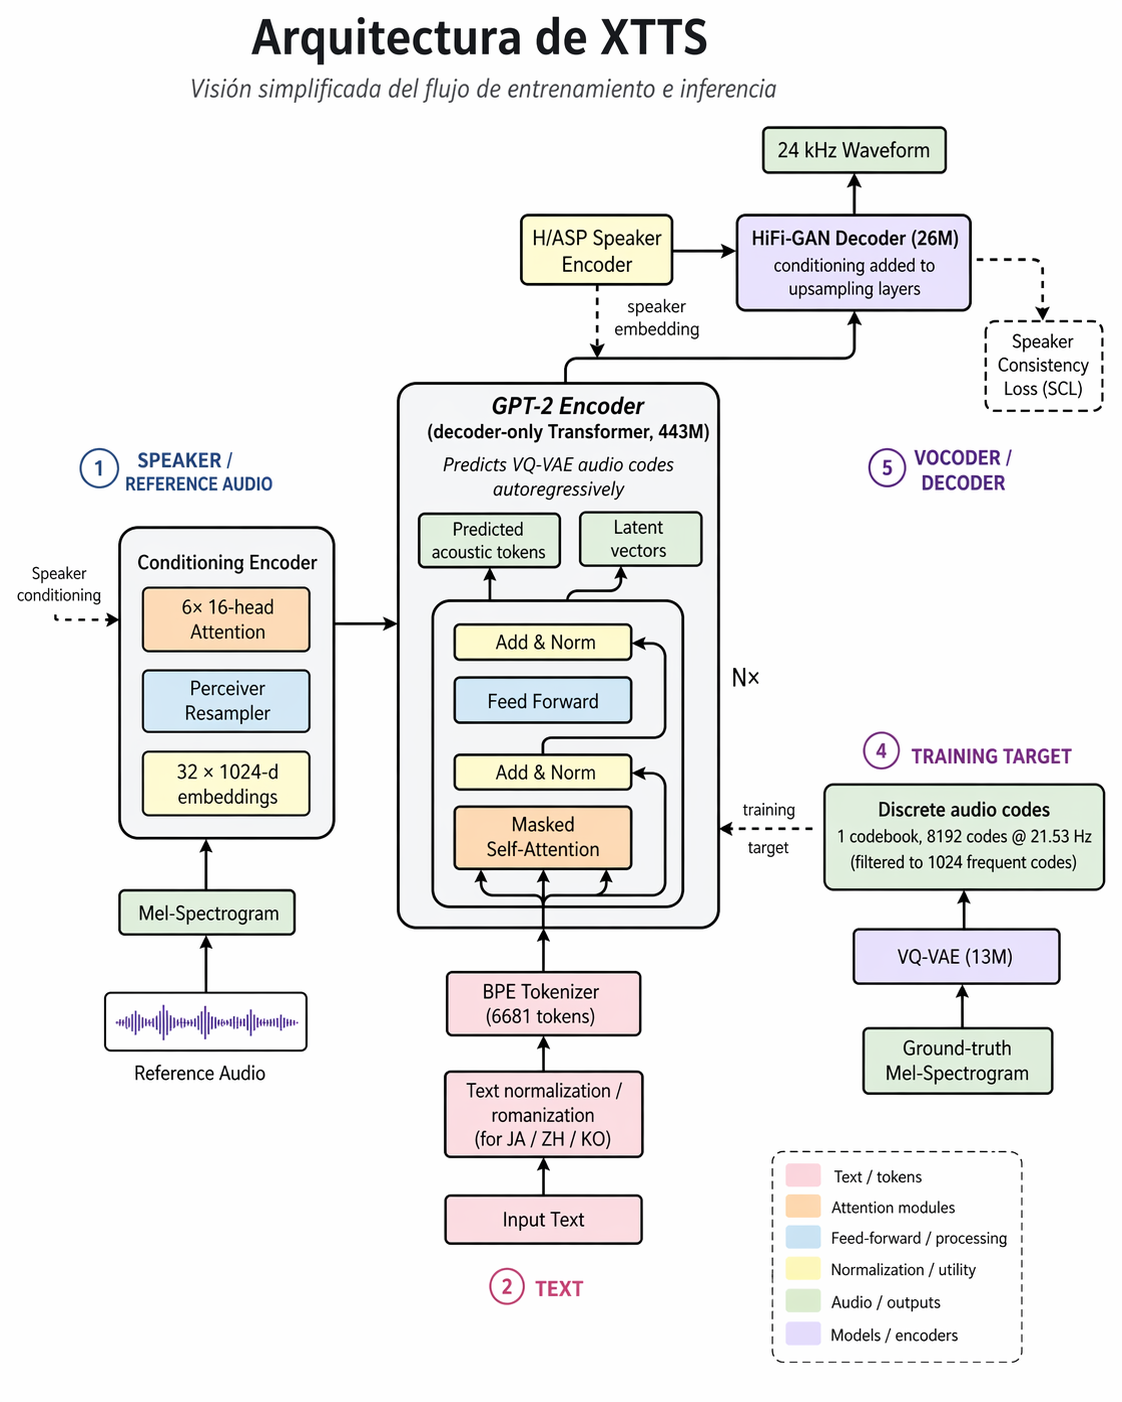
\includegraphics[width=0.9\textwidth]{Imagenes/Propias/Xtts.png}
    \caption[Diagrama general del flujo de XTTS]{
    Diagrama general del flujo de XTTS a partir de texto de entrada y audio de referencia. Fuente: elaboración propia asistida por GPT-Images-2.0 de OpenAI.
    }
    \label{fig:xtts-arquitectura}
\end{figure}

Esta arquitectura permite generar una voz condicionada por una referencia corta de audio, manteniendo cierta identidad del hablante sin necesidad de entrenar un modelo específico desde cero para cada comentarista.

\subsection{Papel de la síntesis de voz dentro del pipeline}

En el contexto de este proyecto, la síntesis de voz transforma los comentarios generados por el modelo de lenguaje en una narración audible. Esta fase cierra el flujo del sistema, convirtiendo eventos detectados y comentarios textuales en audio sincronizable con el vídeo.

En una tarea de narración deportiva, no basta con que la voz generada sea inteligible. También resultan importantes la latencia, la expresividad, la naturalidad en español y la capacidad de mantener un estilo consistente. Por este motivo, el módulo de TTS debe producir audio con suficiente calidad, pero también con un coste temporal asumible dentro del pipeline.

La implementación concreta del módulo de síntesis de voz se describe posteriormente en la \hyperref[sec:sintesis-voz-pipeline]{Sección~\ref*{sec:sintesis-voz-pipeline}}.

\chapter{Trabajo Relacionado}
\label{cap:trabajoRelacionado}

En este capítulo se revisan trabajos y enfoques relacionados con los principales módulos del sistema desarrollado. Dado que el proyecto combina varias áreas, el análisis no se limita a una única línea de investigación, sino que se organiza según las fases más relevantes del pipeline: detección de jugadores y balón, tracking multiobjeto y detección de eventos futbolísticos.

El objetivo de esta revisión es contextualizar las decisiones técnicas adoptadas en el proyecto, identificar alternativas existentes y señalar las principales dificultades asociadas a cada tarea. De este modo, el capítulo sirve como puente entre las tecnologías introducidas previamente y la descripción concreta del sistema implementado.


\section{Detección de jugadores y balón en fútbol}

La detección de objetos es una de las primeras fases necesarias para cualquier sistema automático de análisis de fútbol, ya que permite localizar en cada frame los elementos relevantes del juego, como jugadores, porteros, árbitros y balón.

Diversos trabajos han abordado este problema como una fase previa para tareas de análisis más complejas. \citet{KomorowskiFootAndBall2020} proponen FootAndBall, un detector conjunto de jugadores y balón orientado específicamente al dominio futbolístico. Este tipo de propuestas muestra que la detección del balón requiere una atención especial, al tratarse de un objeto pequeño, visualmente ambiguo y con frecuentes pérdidas de detección en cámaras broadcast.

Frente a YOLO, una alternativa clásica son los detectores de dos etapas, como Faster R-CNN. Este método propuesto por \citet{RenFasterRCNN2015} introduce una red de propuesta de regiones, o \textit{Region Proposal Network}, para generar zonas candidatas antes de clasificarlas y refinar sus cajas. Esta estrategia suele ofrecer detecciones precisas, pero implica un coste computacional mayor y una arquitectura menos directa para un pipeline de vídeo que debe ejecutarse frame a frame.

Otra alternativa reciente son los detectores basados en Transformers. DETR \citep{CarionDETR2020} introdujo una formulación de la detección como predicción directa de un conjunto de objetos, eliminando la necesidad de muchos componentes heurísticos habituales en detectores clásicos. Sobre esta línea, RF-DETR \citep{RobinsonRFDETR2026} plantea una variante orientada a detección en tiempo real, buscando un compromiso entre precisión y latencia. Este tipo de modelos resulta interesante como alternativa moderna a YOLO, ya que las arquitecturas basadas en Transformers pueden capturar relaciones globales entre objetos y adaptarse bien a dominios nuevos.

En este proyecto se opta por YOLO, descrito con más detalle en la \hyperref[sec:yolo-tecnologias]{Sección~\ref*{sec:yolo-tecnologias}}, por su madurez práctica, disponibilidad de herramientas de \textit{fine-tuning}, integración sencilla con el resto del pipeline y buen equilibrio entre velocidad y precisión en vídeo.
\section{Tracking multiobjeto en vídeo deportivo}

El tracking multiobjeto es una tarea especialmente compleja en fútbol debido a las oclusiones, los cruces entre jugadores, la similitud visual entre compañeros de equipo, los cambios de cámara y las detecciones intermitentes. Estas dificultades han motivado el uso de distintos enfoques de asociación temporal y reidentificación para mantener identidades consistentes a lo largo del vídeo.

Una alternativa habitual es DeepSORT, propuesto por \citet{WojkeDeepSORT2017}, que extiende SORT incorporando descriptores de apariencia aprendidos mediante redes de reidentificación. Además de la predicción de movimiento mediante el filtro de Kalman \citep{Kalman1960}, DeepSORT compara las detecciones con las trayectorias activas utilizando tanto información geométrica como apariencia visual. La \hyperref[fig:deepsort-esquema]{Figura~\ref*{fig:deepsort-esquema}} muestra un esquema general de este funcionamiento.

\begin{figure}[H]
    \centering
    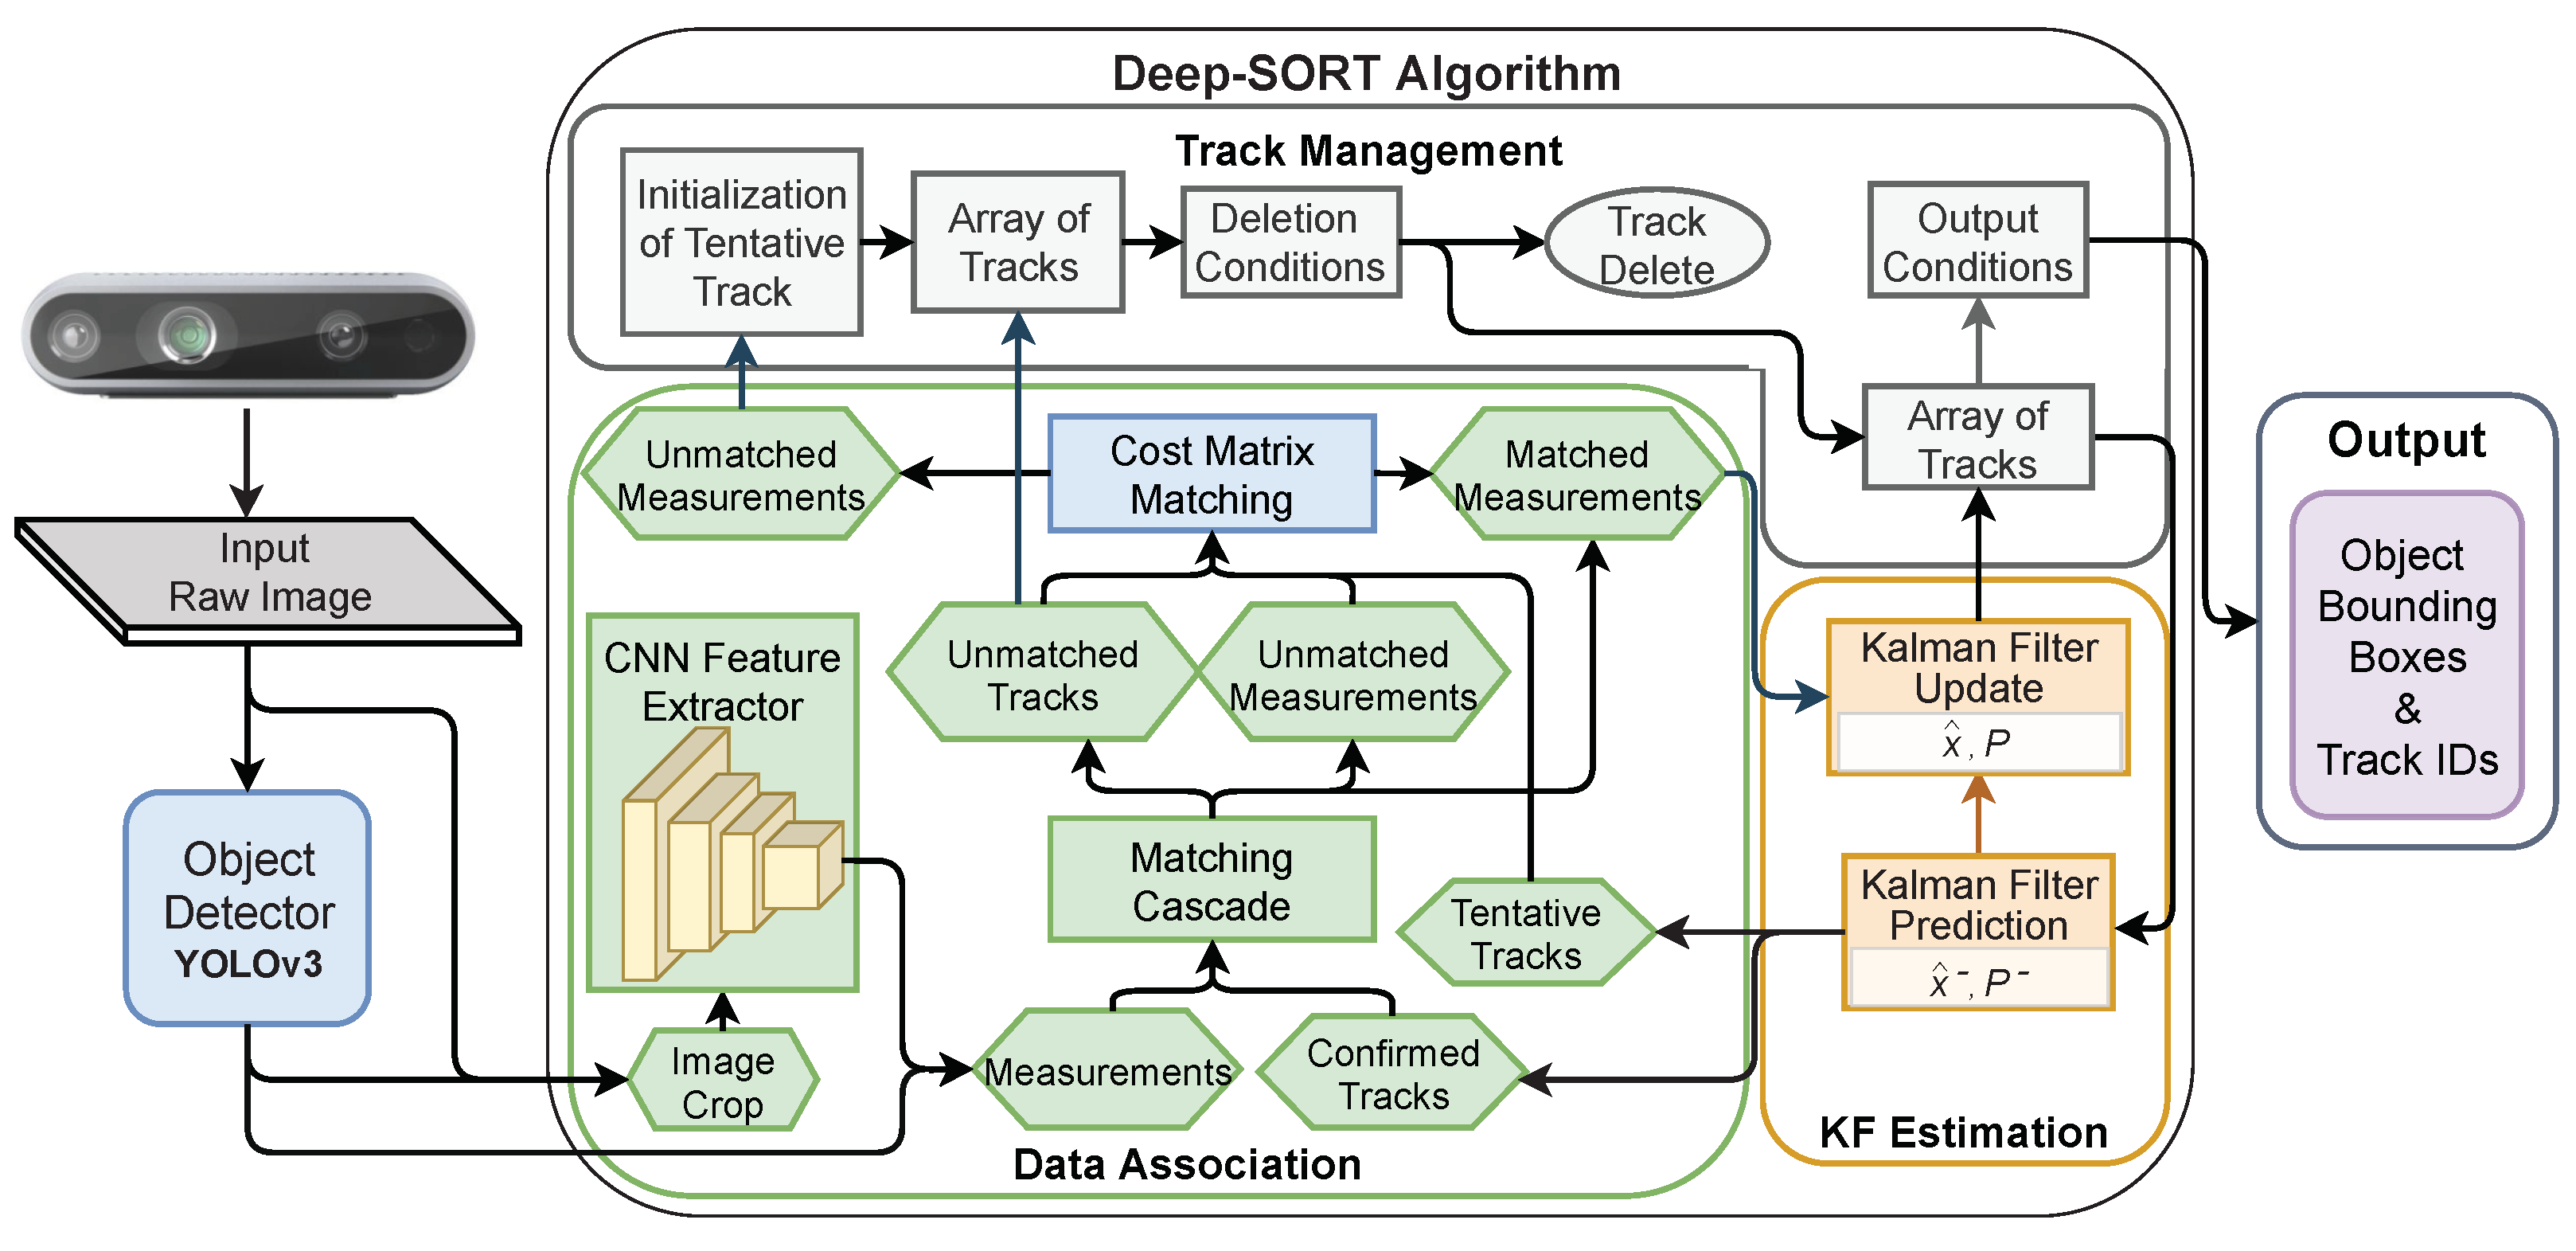
\includegraphics[width=0.9\textwidth]{Imagenes/Propias/DeepSort.png}
    \caption[Esquema general de DeepSORT]{
    Esquema general de DeepSORT. El método combina predicción mediante filtro de Kalman, asociación de detecciones y un descriptor de apariencia obtenido con una red convolucional, lo que ayuda a mantener identidades cuando el movimiento por sí solo no basta. Fuente: reproducido de \citep{PereiraDeepSORT2022}.
    }
    \label{fig:deepsort-esquema}
\end{figure}

Este enfoque puede reducir cambios de identidad en escenarios donde la apariencia visual ayuda a distinguir personas, como vigilancia o seguimiento de peatones. Sin embargo, en fútbol broadcast la apariencia puede ser menos discriminativa, ya que muchos jugadores del mismo equipo llevan equipaciones casi idénticas y las cajas pueden tener baja resolución. Además, entrenar o utilizar descriptores de reidentificación robustos para jugadores concretos requiere datos adicionales que no siempre están disponibles.

Otra alternativa relevante es OC-SORT, propuesto por \citet{CaoOCSORT2023}. Este método revisa el uso del filtro de Kalman en tracking y plantea una asociación más centrada en las observaciones reales, reduciendo errores acumulados durante oclusiones o movimientos no lineales. Este enfoque resulta interesante para deportes, ya que los jugadores no siempre siguen trayectorias suaves y pueden realizar cambios bruscos de dirección.

Frente a estas alternativas, ByteTrack resulta atractivo para sistemas de análisis deportivo por su equilibrio entre simplicidad, eficiencia y robustez ante detecciones de baja confianza. Su enfoque permite recuperar objetos que un tracker convencional podría descartar prematuramente, algo especialmente útil en escenas con oclusiones, agrupaciones de jugadores o detecciones inestables.
\section{Detección de eventos en fútbol}

La detección de eventos en fútbol tiene como objetivo identificar cuándo ocurren acciones relevantes del partido y asignarles una interpretación semántica, como pase, tiro, falta, saque o cambio de posesión. Esta tarea es especialmente compleja porque muchas acciones no pueden reconocerse únicamente a partir de un único frame, sino que dependen de la evolución temporal de jugadores, balón y contexto de juego.

Una línea de trabajo relacionada es el \textit{action spotting}, cuyo objetivo consiste en localizar temporalmente acciones relevantes dentro de vídeos largos de partido. En fútbol, SoccerNet \citep{GiancolaSoccerNet2018} ha sido una de las principales referencias para esta tarea, al proporcionar un amplio dataset de partidos broadcast con anotaciones temporales de eventos. Posteriormente, SoccerNet-v2 \citep{DeliegeSoccerNetV22021} amplió el dataset con anotaciones más densas y nuevas tareas de comprensión de vídeo, incluyendo acciones, cambios de cámara y repeticiones.

En vídeo broadcast, muchos trabajos abordan la detección de acciones directamente a partir de la señal visual. Una línea clásica consiste en combinar extractores convolucionales con modelos temporales: primero se obtiene una representación visual de cada frame mediante una CNN y después se modela la evolución temporal de la secuencia con redes recurrentes o LSTM, como en LRCN \citep{DonahueLRCN2015}. Otra línea emplea arquitecturas espaciotemporales, como I3D \citep{CarreiraI3D2017}, capaces de capturar conjuntamente apariencia y movimiento a partir de convoluciones 3D. Estos enfoques son potentes, pero suelen requerir grandes cantidades de vídeo anotado, diversidad visual y un coste computacional considerable.

Dentro del contexto de SoccerNet, se han propuesto métodos específicos para \textit{action spotting} en fútbol broadcast. \citet{CioppaCALF2020} introducen CALF, una función de pérdida consciente del contexto temporal que permite localizar acciones alrededor de un instante anotado, evitando tratar cada frame de forma completamente aislada. Posteriormente, NetVLAD++ \citep{GiancolaNetVLAD2021} propone una agregación temporal que separa el contexto anterior y posterior a una acción, mejorando la representación de eventos en secuencias largas. Más recientemente, T-DEED \citep{XarlesTDEED2024} busca aumentar la resolución y discriminabilidad temporal de las predicciones para eventos deportivos. Este tipo de métodos resulta especialmente relevante para tareas como BAS (\textit{Ball Action Spotting}), donde se pretende detectar acciones relacionadas con el balón directamente desde el vídeo.

Frente a los enfoques basados principalmente en frames RGB, PathCRF \citep{KimPathCRF2026} plantea una alternativa basada en trayectorias estructuradas de jugadores. Como se describe con más detalle en la \hyperref[sec:pathcrf-tecnologias]{Sección~\ref*{sec:pathcrf-tecnologias}}, el modelo infiere una secuencia de estados de posesión y extrae eventos a partir de sus cambios. Su entrenamiento y evaluación se apoyan en el \textit{Sportec Open DFL Dataset}, publicado por \citet{BassekIntegratedDataset2025}, que proporciona eventos anotados y datos posicionales oficiales de partidos de la Bundesliga.

En resumen, métodos como LRCN, I3D, CALF, NetVLAD++ o T-DEED representan enfoques consolidados para detectar eventos desde vídeo broadcast. Sin embargo, PathCRF resulta especialmente interesante para pipelines que ya construyen una representación geométrica y temporal del partido, ya que permite transformar trayectorias de jugadores en eventos semánticos utilizables por etapas posteriores.
\chapter{Procesamiento Visual}
\label{cap:procesamientoVisual}

En los capítulos anteriores se ha presentado una visión general del proyecto, las principales tecnologías utilizadas y los trabajos relacionados más relevantes. A partir de este capítulo comienza la descripción del sistema desarrollado, organizada siguiendo las grandes fases del pipeline.

Este capítulo se centra en la primera parte del sistema: el procesamiento visual del vídeo broadcast. Su objetivo es transformar los frames originales del partido en una representación estructurada de los elementos del juego. Para ello se describen las etapas de detección de jugadores, árbitros, porteros y balón, la identificación de equipos, la estimación geométrica sobre el terreno de juego y el tracking multiobjeto empleado para mantener identidades consistentes a lo largo del vídeo.

La salida de este bloque visual sirve como base para los capítulos posteriores, donde se analizan aspectos futbolísticos de mayor nivel, como la posesión, las posiciones de los jugadores y los eventos del partido, en el \hyperref[fig:arquitectura-software]{Capítulo~\ref*{cap:analisisTactico}} , y finalmente se genera la narración automática en texto y audio, descrita en el \hyperref[cap:narracion]{Capítulo~\ref*{cap:narracion}}.

Antes de entrar en cada etapa, resulta útil tener en mente un frame del vídeo original, es decir, la entrada del sistema antes de aplicar cualquier tipo de procesamiento. La \hyperref[fig:raw-football-image]{Figura~\ref*{fig:raw-football-image}} muestra un ejemplo de frame de entrada utilizado por el pipeline.

\begin{figure}[H]
    \centering
    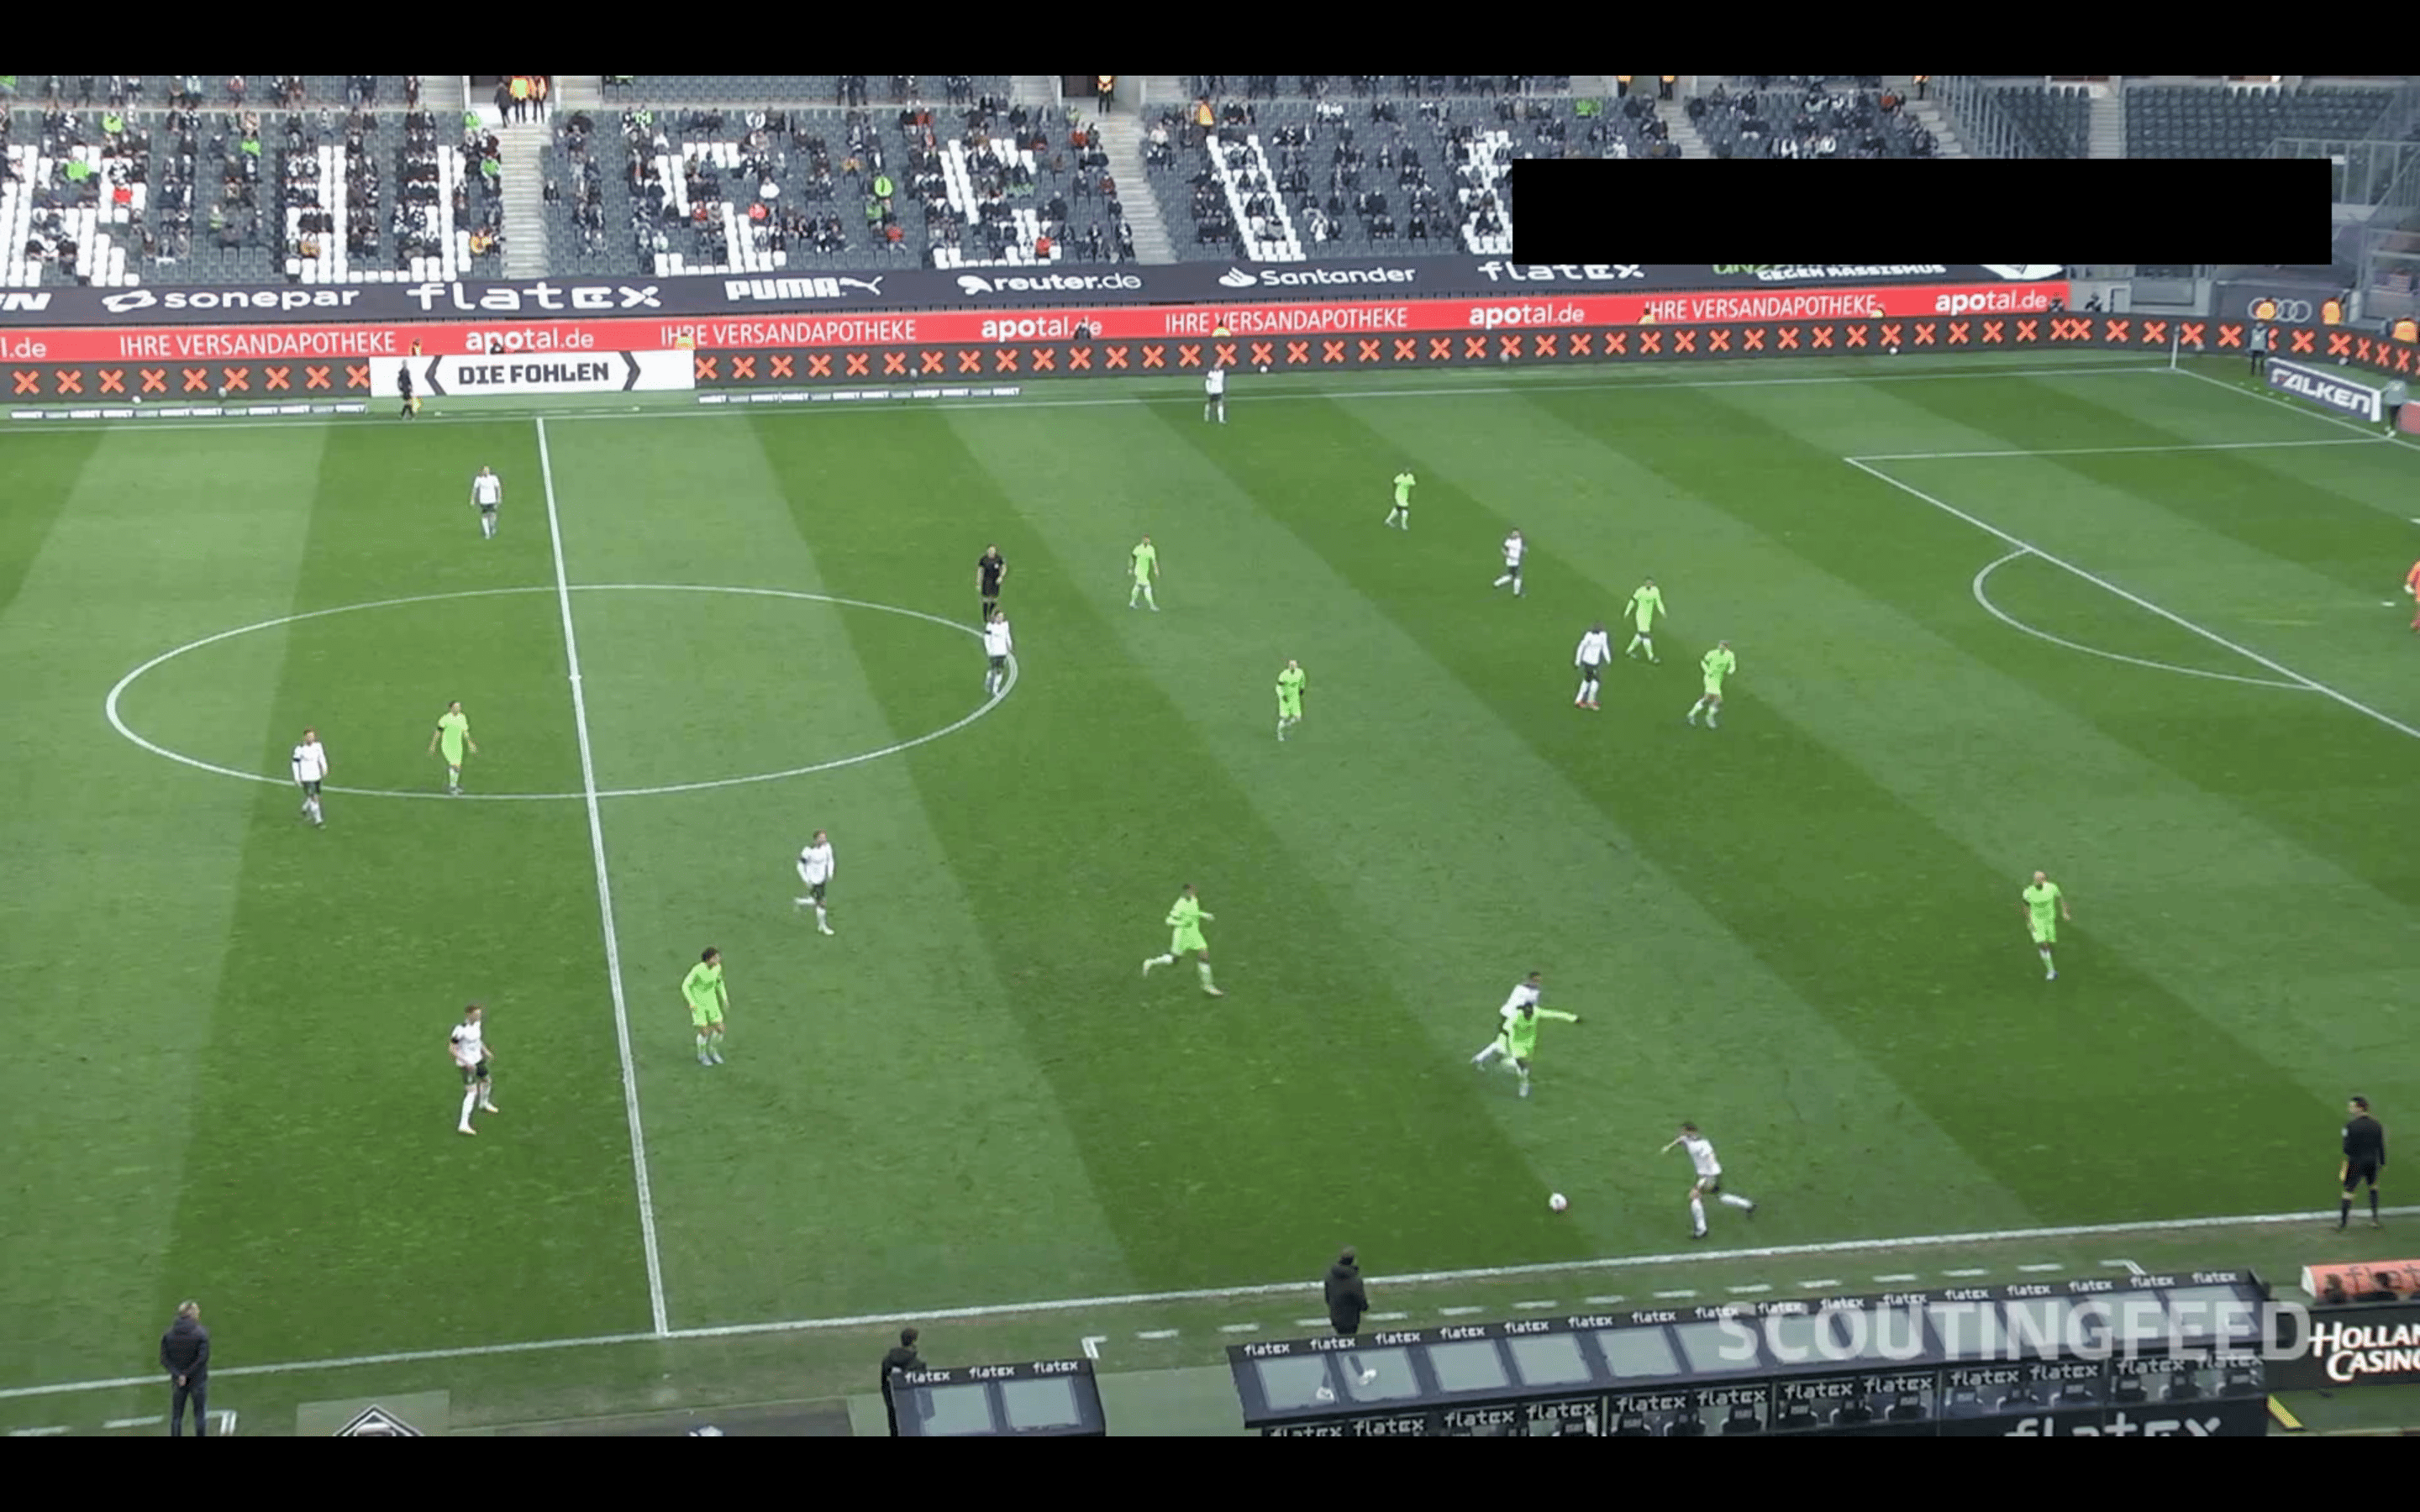
\includegraphics[width=0.9\textwidth]{Imagenes/Propias/Raw_image.png}
    \caption[Frame original del vídeo de entrada]{
    Frame original del vídeo de entrada antes de aplicar detección, calibración, identificación de equipos o tracking.
    }
    \label{fig:raw-football-image}
\end{figure}


\section{Detección de elementos del juego}
\label{sec:deteccion-elementos-juego}

La primera fase del pipeline consiste en detectar, fotograma a fotograma, los elementos relevantes del partido. Para esta tarea se empleó YOLOv11m, donde la letra \texttt{m} hace referencia a la variante \textit{medium}, elegida por ofrecer un compromiso razonable entre precisión y coste computacional.

Como punto de partida se utilizó el modelo base, es decir, el modelo preentrenado sin adaptación específica al dominio futbolístico. Al aplicarlo directamente sobre vídeo de fútbol, el modelo detecta jugadores, árbitros y porteros principalmente como instancias de la clase \texttt{person}, mientras que el balón puede aparecer como \texttt{sports ball}. Esto puede observarse en la \hyperref[fig:raw-detection-yolo11m]{Figura~\ref*{fig:raw-detection-yolo11m}}. Esta salida inicial permite comprobar que el detector reconoce objetos relevantes en la escena, pero no proporciona todavía la separación semántica necesaria para el proyecto, ya que agrupa todos los participantes humanos en una misma clase.

\begin{figure}[H]
    \centering
    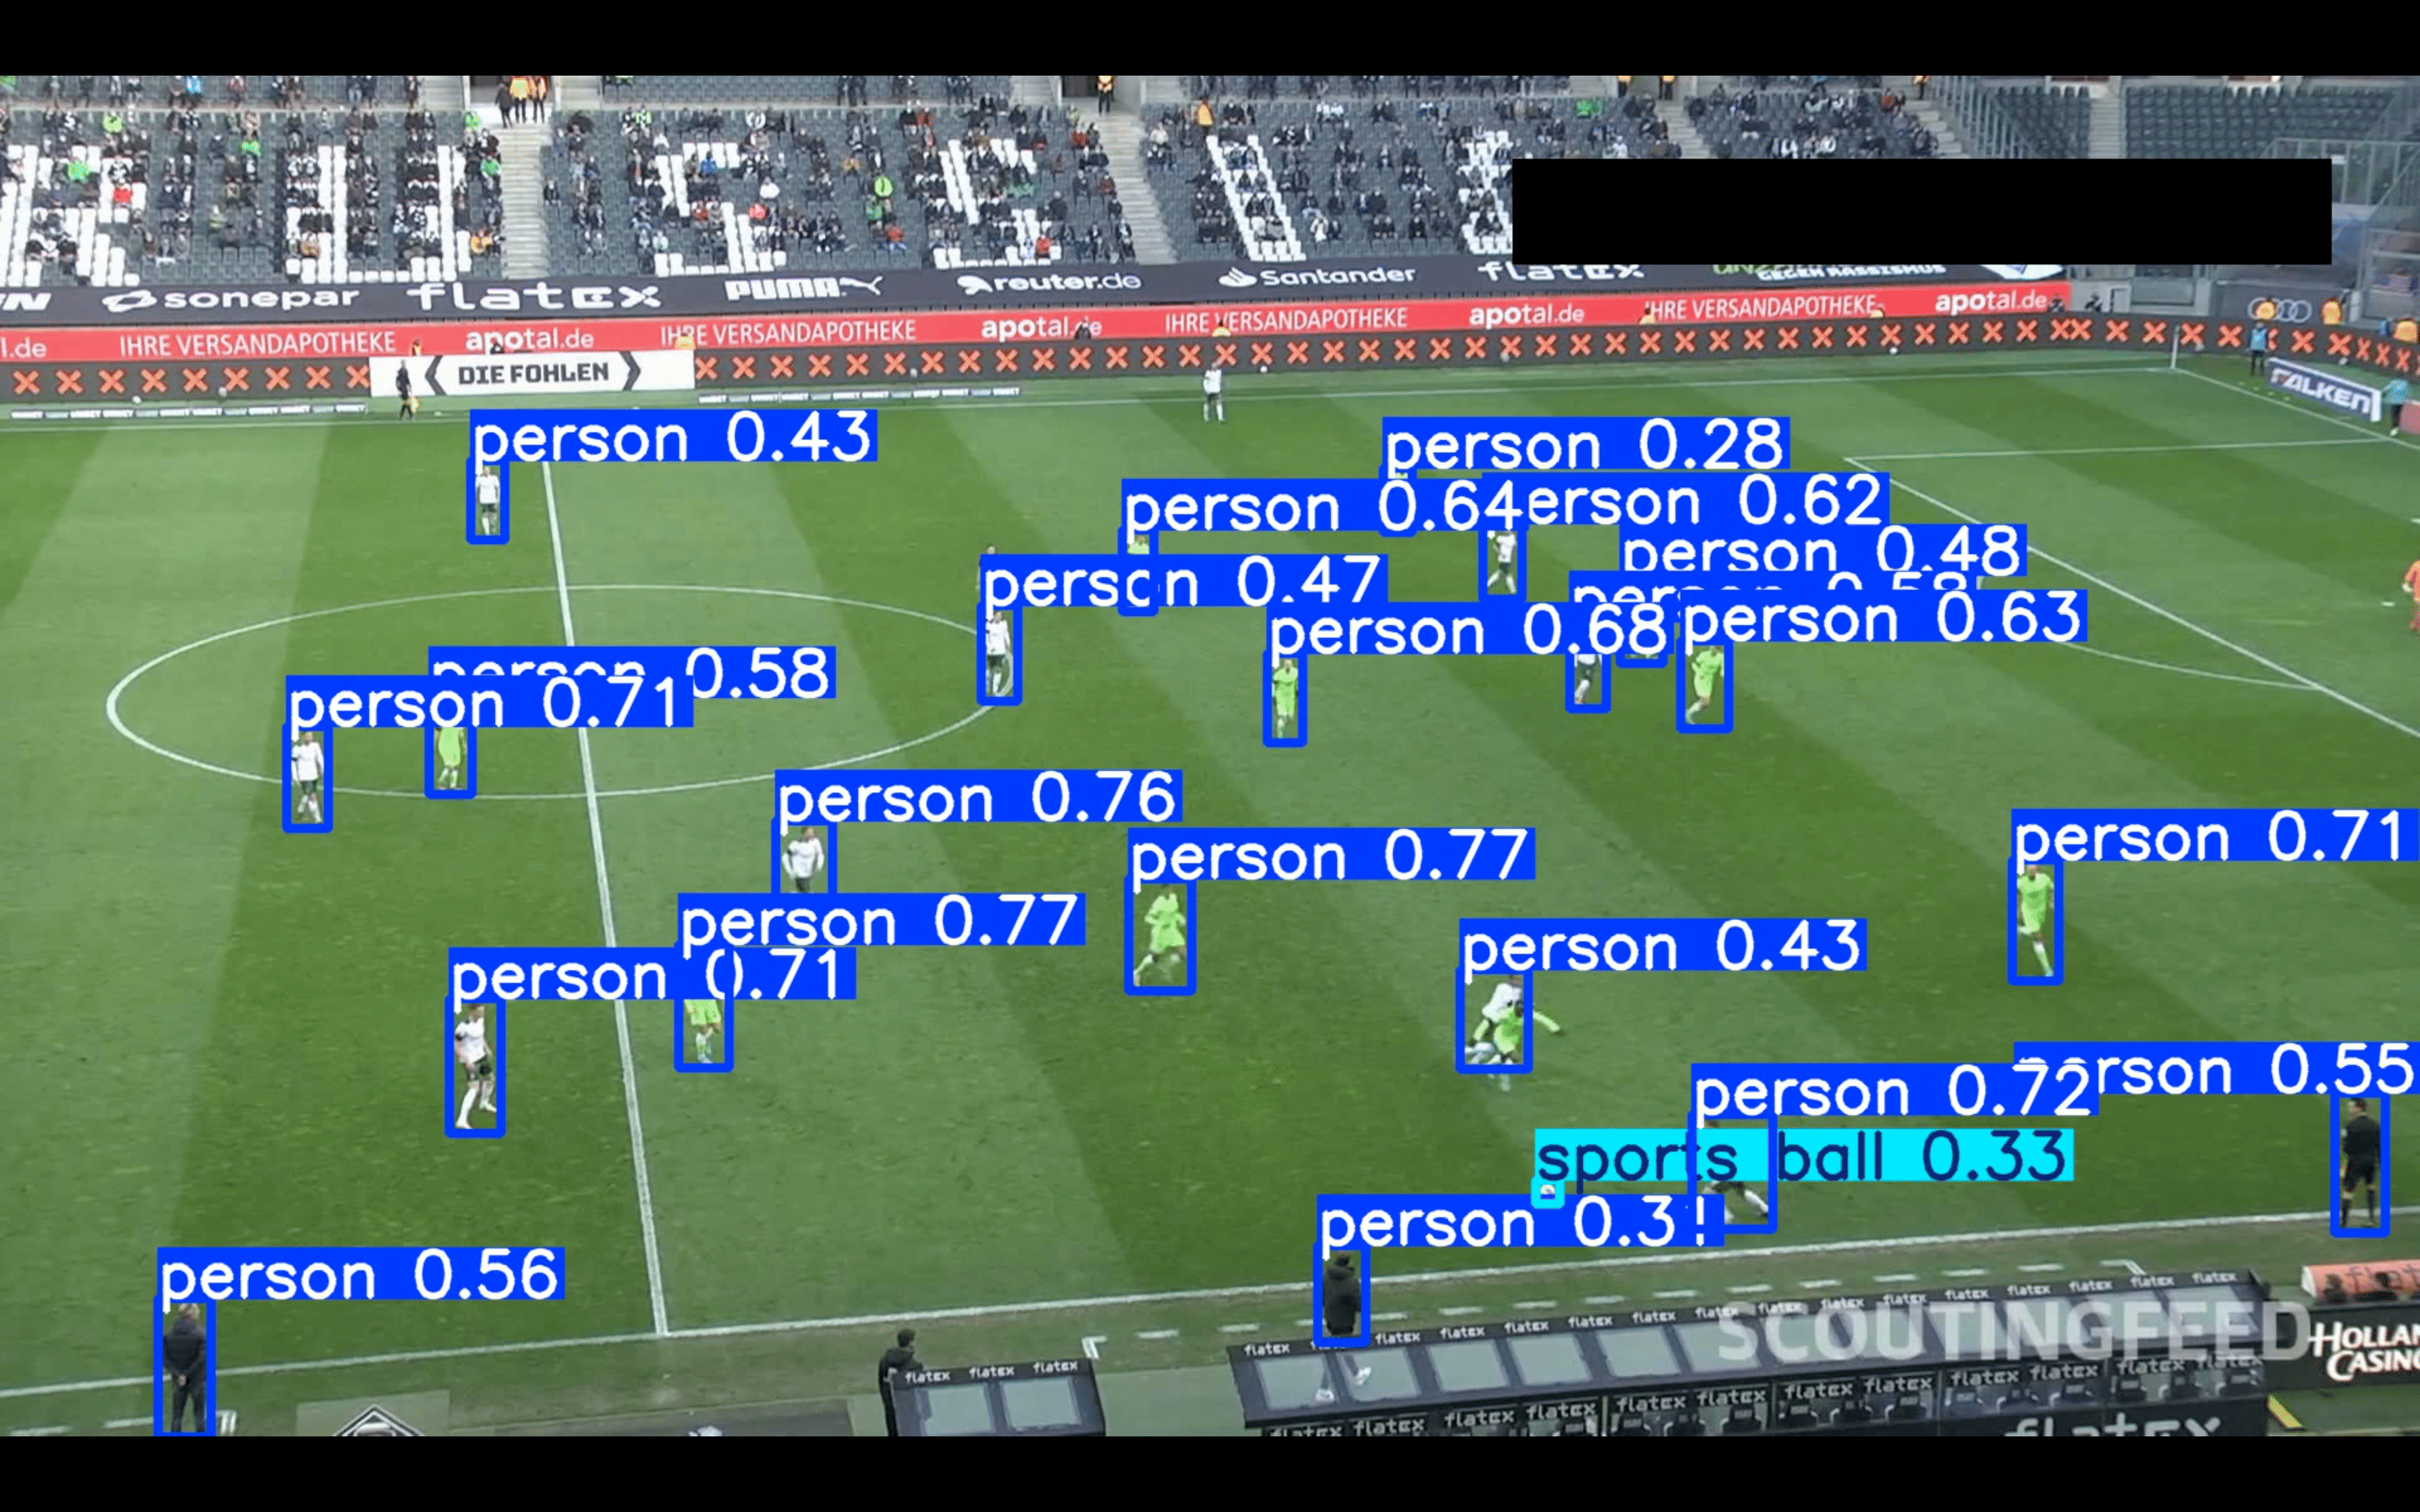
\includegraphics[width=0.9\linewidth]{Imagenes/Propias/Raw_detection.png}
    \caption[Detección inicial con YOLOv11m]{Detección inicial realizada con YOLOv11m base sobre un frame del partido.}
    \label{fig:raw-detection-yolo11m}
\end{figure}

Para observar el comportamiento del modelo base se realizó una prueba exploratoria sobre un clip corto de 10 frames. YOLO proporciona para cada detección un valor de confianza (\textit{confidence}), que representa la seguridad estimada del modelo respecto a la clase predicha. Los resultados se muestran en la Tabla \ref{tab:yolo11mBaseFrame}.

\begin{table}[H]
	\centering
	\begin{tabular}{c|c|c|c|c}
		\textbf{Frame} & \textbf{Personas} & \textbf{Balón} & \textbf{Conf. media} & \textbf{Conf. max} \\
		\hline\hline
		1 & 22 & 0 & 0.5646 & 0.7637 \\
		2 & 22 & 0 & 0.5741 & 0.7864 \\
		3 & 22 & 0 & 0.5724 & 0.7894 \\
		4 & 23 & 1 & 0.5370 & 0.7900 \\
		5 & 23 & 1 & 0.5094 & 0.7775 \\
		6 & 23 & 0 & 0.5514 & 0.7846 \\
		7 & 23 & 0 & 0.5571 & 0.7727 \\
		8 & 21 & 1 & 0.5781 & 0.7730 \\
		9 & 20 & 1 & 0.6162 & 0.7941 \\
		10 & 19 & 1 & 0.5925 & 0.7862 \\
		\hline
	\end{tabular}
	\caption[Prueba exploratoria de detección con YOLOv11m]{Prueba exploratoria de detección con YOLOv11m base sobre un clip corto de 10 frames.}
	\label{tab:yolo11mBaseFrame}
\end{table}

Los resultados muestran que el modelo detecta de forma estable a las personas presentes en la escena, con entre 19 y 23 detecciones por frame. Sin embargo, la detección del balón resulta más irregular, ya que solo aparece en 5 de los 10 frames analizados.

Sin embargo, para este proyecto no basta con detectar personas genéricas: es necesario distinguir entre elementos futbolísticos concretos, como jugadores, árbitros, porteros y balón. Por este motivo se decidió adaptar el detector mediante \textit{fine-tuning}.

\subsection{Adaptación del detector mediante \textit{fine-tuning}}
Como el modelo YOLOv11m base no proporcionaba la separación semántica necesaria para el proyecto, se decidió adaptar el detector al dominio futbolístico mediante \textit{fine-tuning}. El objetivo era que el modelo no solo detectara personas genéricas, sino que distinguiera entre clases relevantes para el sistema, como jugadores, árbitros, porteros y balón.


\subsubsection{Conjuntos de datos utilizados}

Para esta adaptación se emplearon tres conjuntos de datos con funciones distintas dentro del proceso de entrenamiento. La \hyperref[tab:datasets-finetuning-yolo]{Tabla~\ref*{tab:datasets-finetuning-yolo}} resume su procedencia, clases anotadas, tamaño y uso dentro del proyecto.

\begin{table}[H]
\centering
\scriptsize
\renewcommand{\arraystretch}{1.25}
\begin{tabularx}{\textwidth}{
>{\raggedright\arraybackslash}p{2.4cm}
>{\raggedright\arraybackslash}X
>{\raggedright\arraybackslash}p{2.8cm}
>{\raggedright\arraybackslash}p{2.5cm}
>{\raggedright\arraybackslash}X
}
\toprule
\textbf{Dataset} & \textbf{Url} & \textbf{Clases} & \textbf{Tamaño / partición} & \textbf{Uso} \\
\midrule

Roboflow fútbol \label{} &
\href{https://universe.roboflow.com/yolo-atnlh/football-detection-wfhdh}{Roboflow - FootBall Detection Computer Vision Model} &
\texttt{ball}, \texttt{player}, \texttt{referee}, \texttt{goalkeeper} $\rightarrow$ \texttt{player}. &
Train/val/test: 612/38/13 &
Primer \textit{fine-tuning} supervisado con clases futbolísticas. \\

\midrule

Datos sintéticos &
\href{https://research.spiideo.com/login/main.html}{Spiideo SoccerNet SynLoc} &
\texttt{person} $\rightarrow$ \texttt{player}. &
Train/val/test: 42.554/6.777/9.309 &
Adaptación intermedia sintética al dominio futbolístico: césped, jugadores, variación de cámara, iluminación y desenfoque de movimiento.. \\

\midrule

DFL-Bundesliga &
\href{https://universe.roboflow.com/inkyu-sa-e0c78/dfl-bundesliga-soccer-football-gpqdy}{Roboflow - DFL-Bundesliga} &
\texttt{ball}, \texttt{player}, \texttt{referee}. &
Train/val/test: 19.068/2.434/2.455 &
Refinamiento final sobre datos reales más próximos al escenario objetivo. \\

\bottomrule
\end{tabularx}
\caption[Conjuntos de datos utilizados para el fine-tuning del detector]{
Conjuntos de datos utilizados durante la adaptación del detector YOLOv11m al dominio futbolístico.
}
\label{tab:datasets-finetuning-yolo}
\end{table}

\noindent\textit{Nota:} Para homogeneizar el entrenamiento entre fases, las clases se adaptaron al formato final del detector: \texttt{player}, \texttt{referee} y \texttt{ball}. En SoccerSynth-Detection, la clase original \texttt{person} se mapeó a \texttt{player}; las clases \texttt{referee} y \texttt{ball} se incluyeron en la definición de clases, aunque no tenían instancias anotadas en ese conjunto. En el dataset Roboflow fútbol, la clase \texttt{goalkeeper} se integró dentro de \texttt{player}.

\subsubsection{Estrategias de entrenamiento}

Se exploraron dos estrategias principales de adaptación. La primera consistió en entrenar YOLOv11m directamente sobre el pequeño dataset \textit{Roboflow fútbol} obtenido en Roboflow. Este dataset permitía introducir clases futbolísticas concretas, como \texttt{ball}, \texttt{player}, \texttt{referee} y \texttt{goalkeeper}, y servía como primer intento de especialización del modelo base. Además, el proyecto de Roboflow incluía un modelo de referencia con métricas publicadas de \textit{mAP@50} del 82.1\%, precisión del 96.7\% y recall del 75.2\%. Estas métricas no se interpretan como resultados propios ni como una evaluación del dataset, sino como un indicio inicial de que las anotaciones y la definición de clases podían ser útiles para adaptar el detector al dominio futbolístico.

La segunda estrategia consistió en un \textit{fine-tuning} secuencial. En primer lugar, el modelo se entrenó sobre SoccerSynth-Detection \citep{SoccerSynthDetection2025}, un conjunto sintético orientado a detección en fútbol. Esta fase tenía como objetivo adaptar el detector al dominio visual del fútbol, exponiéndolo a escenas con césped, jugadores, variaciones de cámara, iluminación y desenfoque de movimiento. Posteriormente, el modelo resultante se refinó sobre DFL-Bundesliga, un conjunto de imágenes reales con clases más próximas al problema final: \texttt{ball}, \texttt{player} y \texttt{referee}.

La motivación de esta estrategia secuencial era aprovechar primero la variabilidad controlada de los datos sintéticos y, después, ajustar el modelo sobre datos reales más cercanos al escenario de aplicación. De esta forma, se buscaba mejorar la capacidad de generalización del detector antes de integrarlo en el pipeline completo.

\subsubsection{Resultados del \textit{fine-tuning} secuencial} 

La \hyperref[fig:results_finetuning_compare]{Figura~\ref*{fig:results_finetuning_compare}} muestra las curvas de entrenamiento de las dos fases del \textit{fine-tuning} secuencial. En la fase sintética, las métricas convergen rápidamente y se estabilizan hacia la mitad del entrenamiento, alcanzando un mAP@50-95 final cercano a 0.80. En la fase DFL-Bundesliga, la mejora es más gradual y las métricas finales son menores, con un mAP@50-95 cercano a 0.63.

\begin{figure}[H]
\centering

\begin{minipage}{0.95\textwidth}
    \centering
    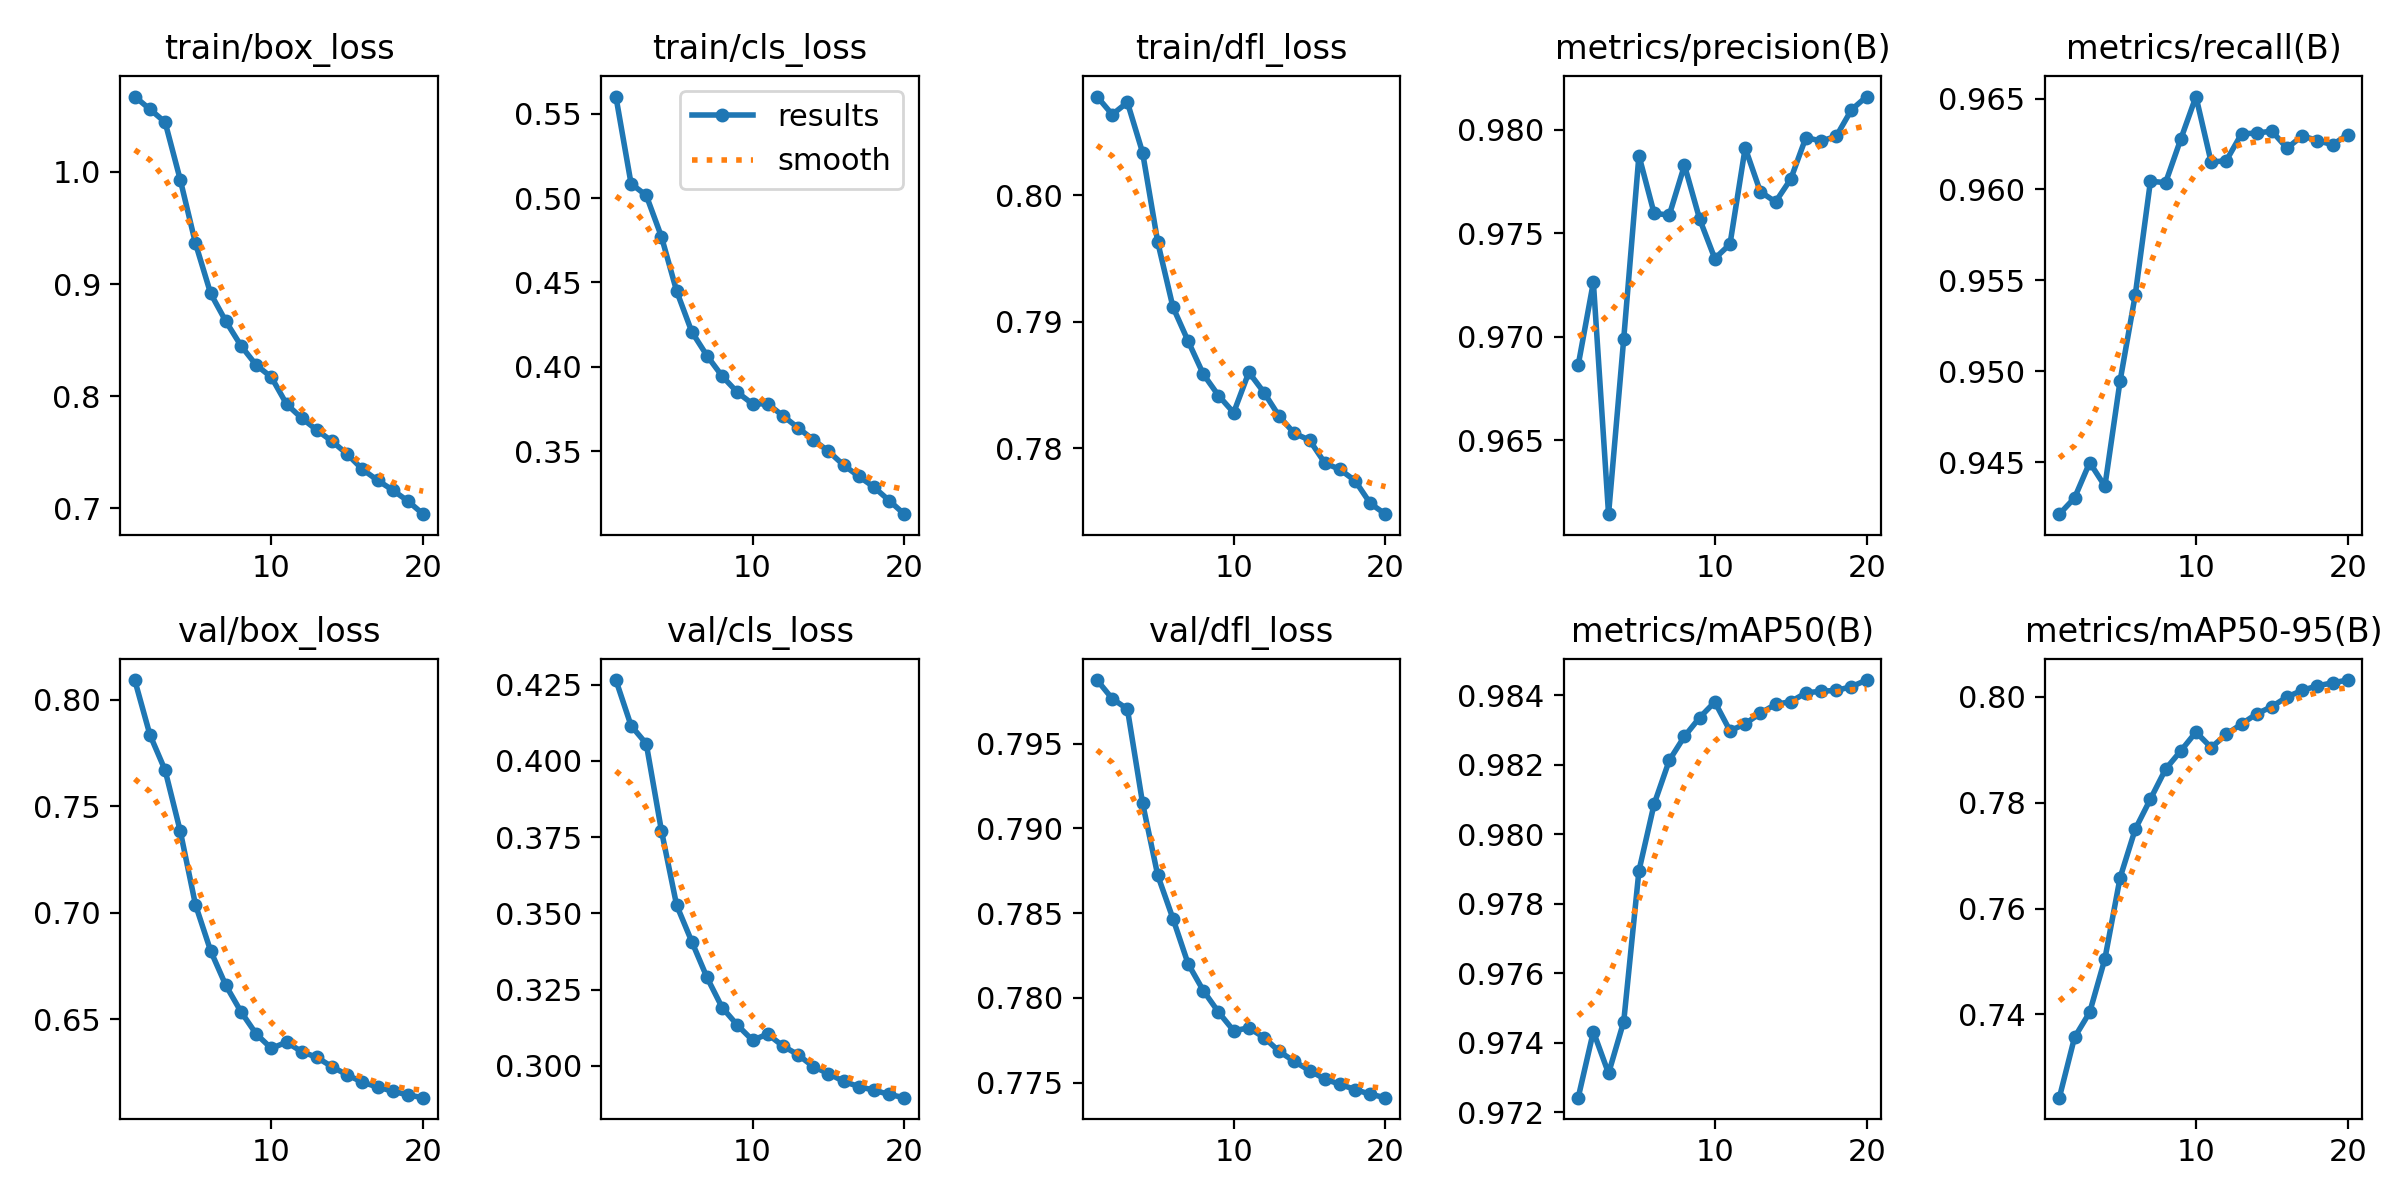
\includegraphics[width=\textwidth]{Imagenes/Propias/results_sinteticos.png}
    \small \textbf{(a)} Primera fase del \textit{fine-tuning} secuencial sobre SoccerSynth-Detection.
\end{minipage}

\vspace{0.4cm}

\begin{minipage}{0.95\textwidth}
    \centering
    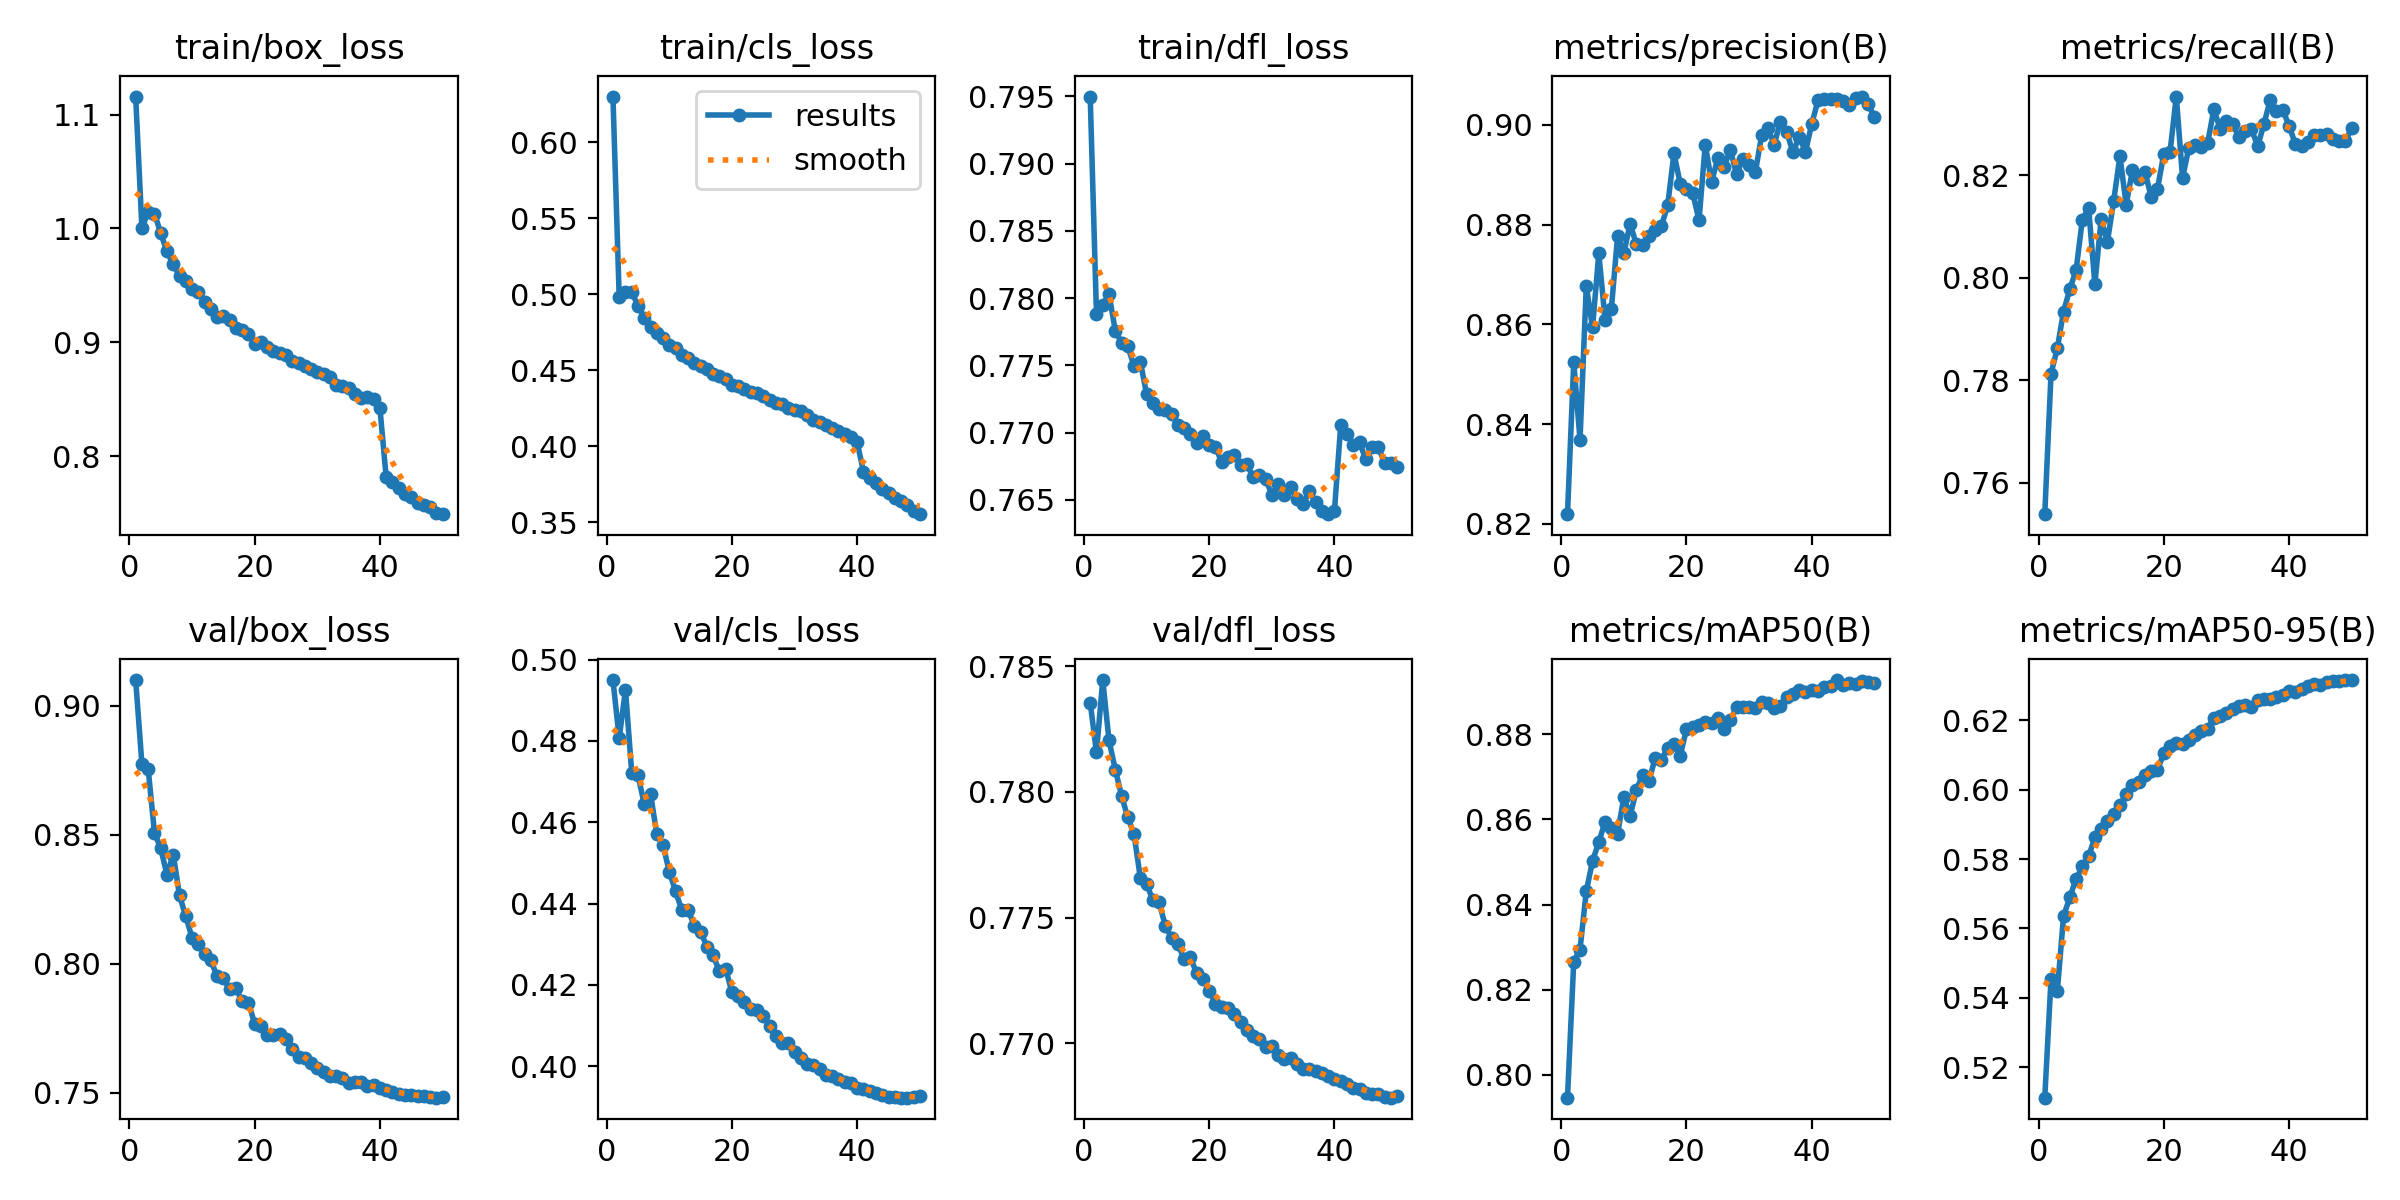
\includegraphics[width=\textwidth]{Imagenes/Propias/results_dfl.png}
    \small \textbf{(b)} Segunda fase del \textit{fine-tuning} secuencial sobre DFL-Bundesliga.
\end{minipage}

\caption[Curvas de entrenamiento del fine-tuning secuencial]{
Curvas de entrenamiento del proceso de \textit{fine-tuning} secuencial.
}
\label{fig:results_finetuning_compare}
\end{figure}

La \hyperref[tab:comparacion_modelos_finetuneados]{Tabla~\ref*{tab:comparacion_modelos_finetuneados}} resume las métricas finales de ambas fases, evaluadas sobre sus respectivos conjuntos de validación. Aunque las métricas de la fase sintética son superiores, no deben interpretarse como una comparación directa entre modelos equivalentes, ya que cada fase utiliza un conjunto de datos distinto. La primera fase sintética trabaja sobre una tarea más simple, homogénea y de una sola clase, mientras que la segunda introduce un dominio más realista y clases más específicas.

\begin{table}[H]
\centering
\scriptsize
\begin{tabular}{c|c|c|c|c|c|c|c}
\textbf{Fase} & \textbf{Ep.} & \textbf{Batch} & \textbf{Imgsz} & \textbf{Prec. final} & \textbf{Recall final} & \textbf{mAP@50} & \textbf{mAP@50-95} \\
\hline\hline
Datos sintéticos & 20 & 8 & 1280 & 0.9816 & 0.9630 & 0.9844 & 0.8032 \\
\hline
DFL-Bundesliga & 50 & 16 & 640 & 0.8911 & 0.8352 & 0.8909 & 0.6305 \\
\hline
\end{tabular}
\caption[Métricas finales del fine-tuning secuencial]{
Métricas finales de validación de las dos fases del \textit{fine-tuning} secuencial.
}
\label{tab:comparacion_modelos_finetuneados}
\end{table}

Para interpretar estas diferencias, la \hyperref[fig:datasets_summary]{Figura~\ref*{fig:datasets_summary}} compara la distribución de clases y las características espaciales de las cajas anotadas en los conjuntos utilizados durante el \textit{fine-tuning} secuencial.

\begin{figure}[H]
\centering

\begin{minipage}{0.55\textwidth}
    \centering
    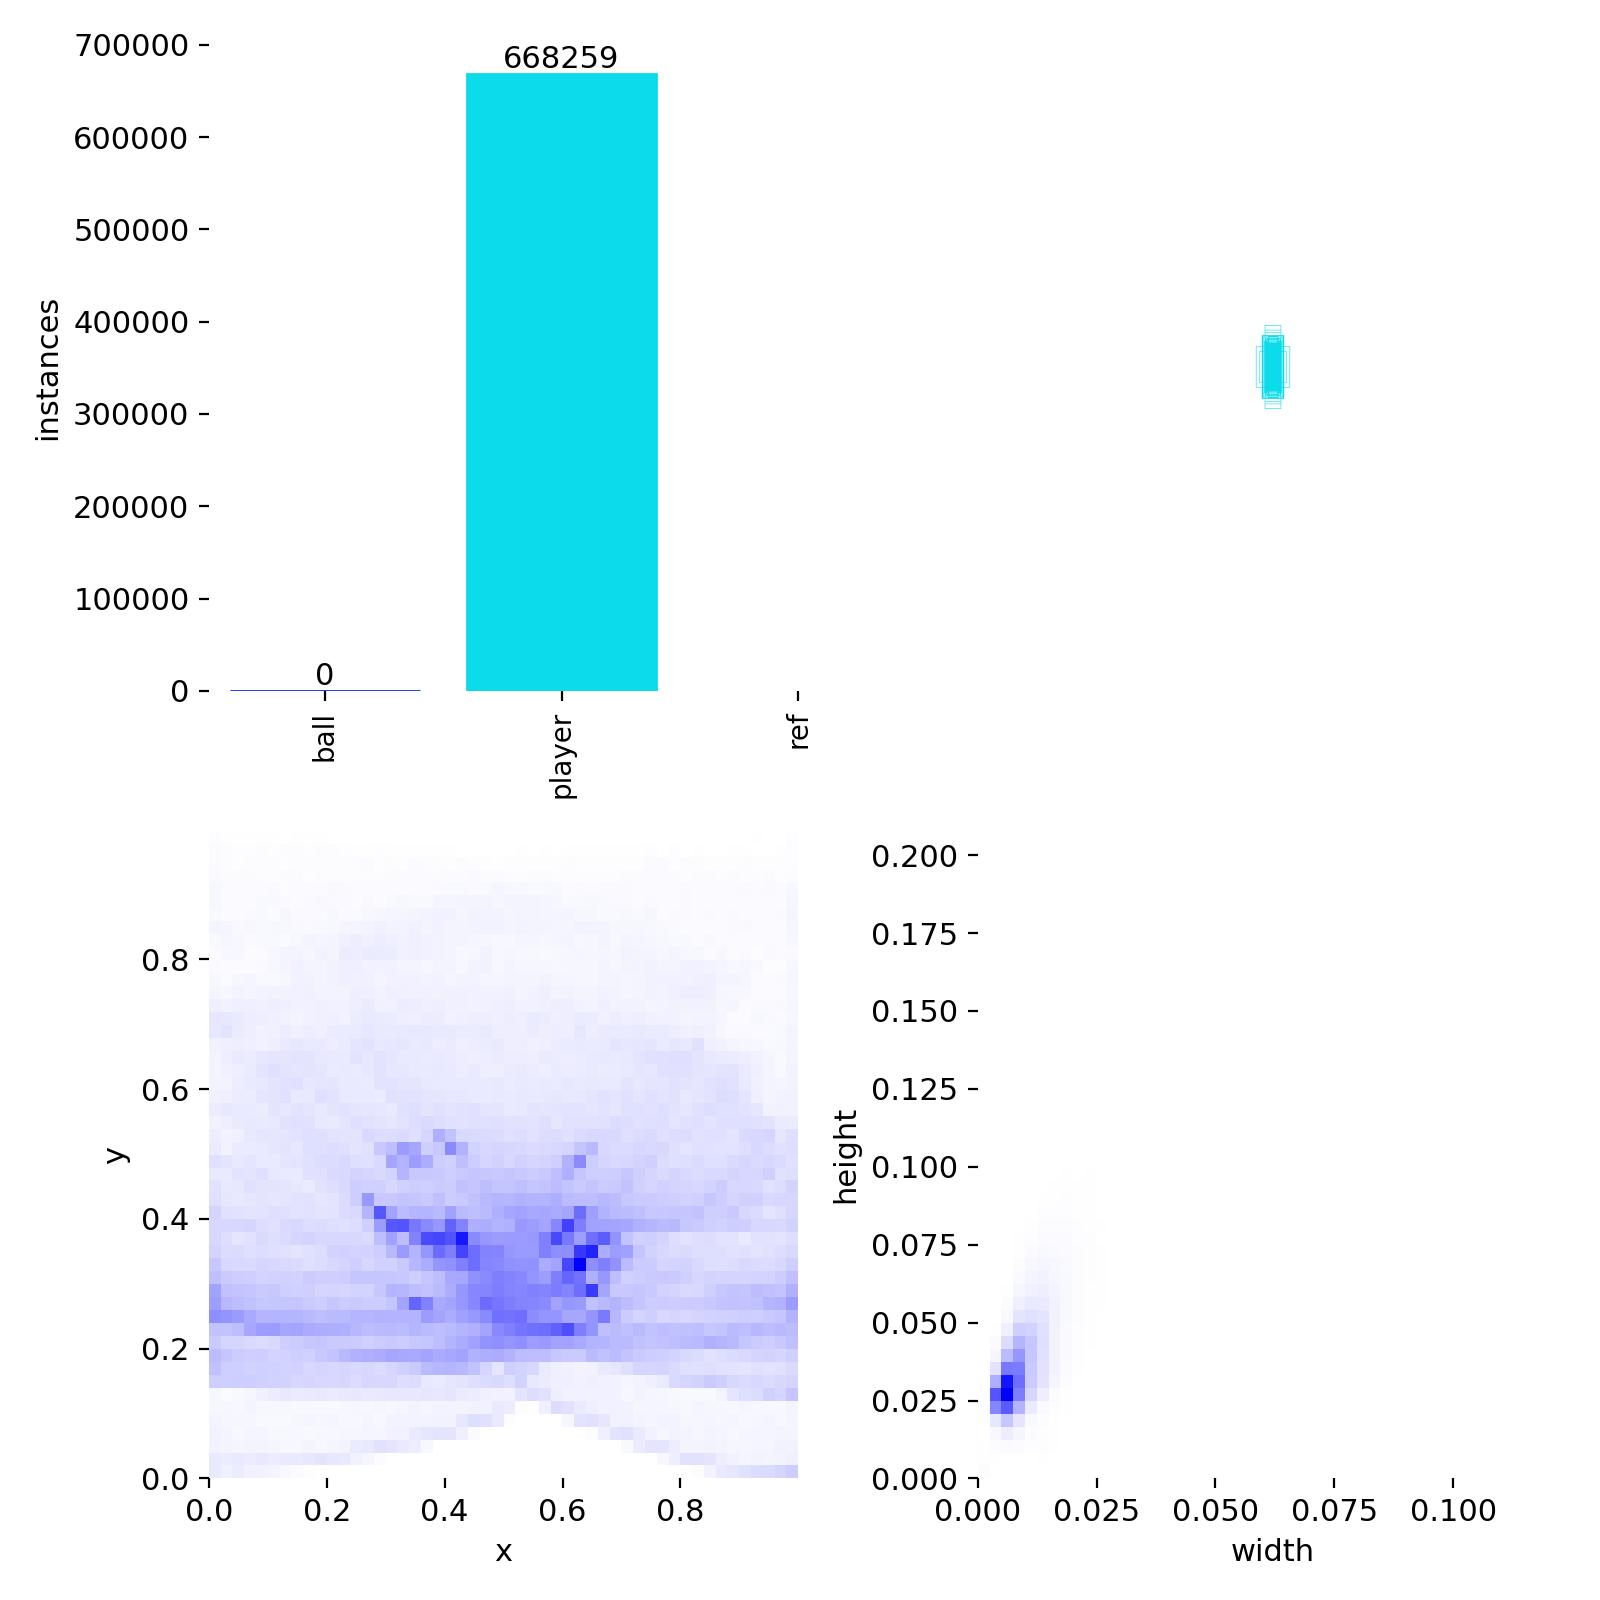
\includegraphics[width=\textwidth]{Imagenes/Propias/labels_sinteticos.jpg}
    \small \textbf{(a)} SoccerSynth-Detection.
\end{minipage}

\vspace{0.4cm}

\begin{minipage}{0.55\textwidth}
    \centering
    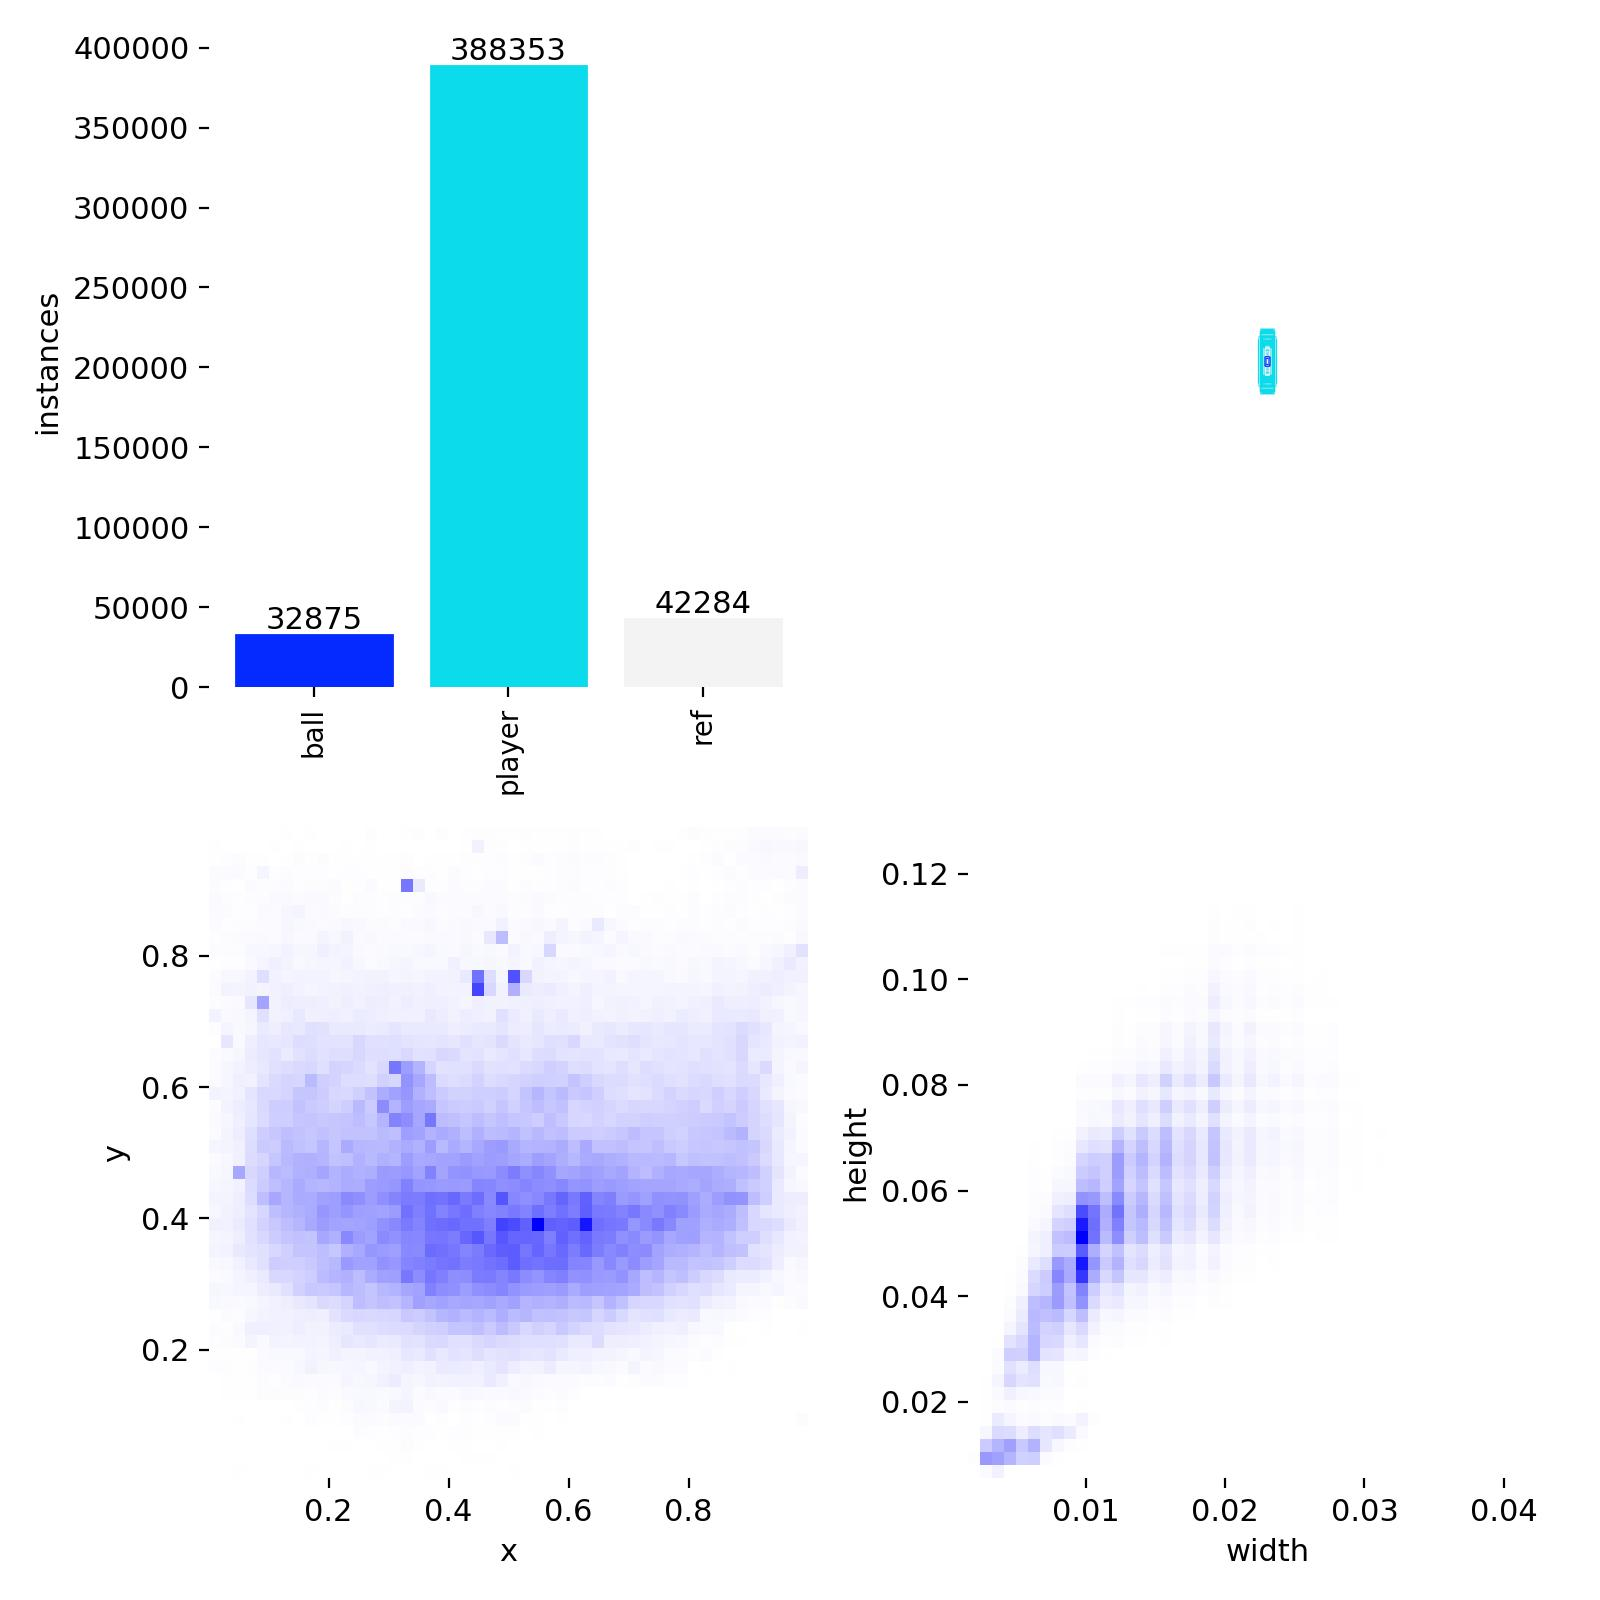
\includegraphics[width=\textwidth]{Imagenes/Propias/labels_dfl.jpg}
    \small \textbf{(b)} Sintéticos + DFL-Bundesliga.
\end{minipage}

\caption[Distribución de etiquetas y cajas en los datasets de fine-tuning]{
Distribución de clases, posiciones normalizadas y tamaños de las cajas delimitadoras en los conjuntos utilizados durante el \textit{fine-tuning} secuencial.
}
\label{fig:datasets_summary}
\end{figure}

Como se aprecia en la \hyperref[fig:datasets_summary]{Figura~\ref*{fig:datasets_summary}}, los datos sintéticos están centrados en la detección de jugadores, mientras que DFL-Bundesliga introduce clases adicionales: balón y árbitro. Por tanto, la segunda fase no solo trabaja sobre imágenes reales, sino también sobre un problema más complejo y desbalanceado. Esto explica que las métricas sean inferiores respecto a la fase sintética sin que ello implique necesariamente un empeoramiento del detector.

La \hyperref[fig:confusion_finetuning_compare]{Figura~\ref*{fig:confusion_finetuning_compare}} muestra las matrices de confusión obtenidas en las dos fases del \textit{fine-tuning} secuencial. En la fase sintética, como ya se había comentado, solo aparece la clase \texttt{player}, con un rendimiento bastante bueno. En la fase DFL-Bundesliga, en cambio, aparecen clases adicionales como \texttt{ball} y \texttt{ref}, lo que permite analizar mejor los errores entre categorías del dominio futbolístico. En particular, se observa que la clase \texttt{player} presenta un comportamiento más estable, mientras que clases menos frecuentes o visualmente más difíciles, como \texttt{ball} y \texttt{ref}, introducen mayor complejidad.

\begin{figure}[H]
\centering

\begin{minipage}{0.55\textwidth}
    \centering
    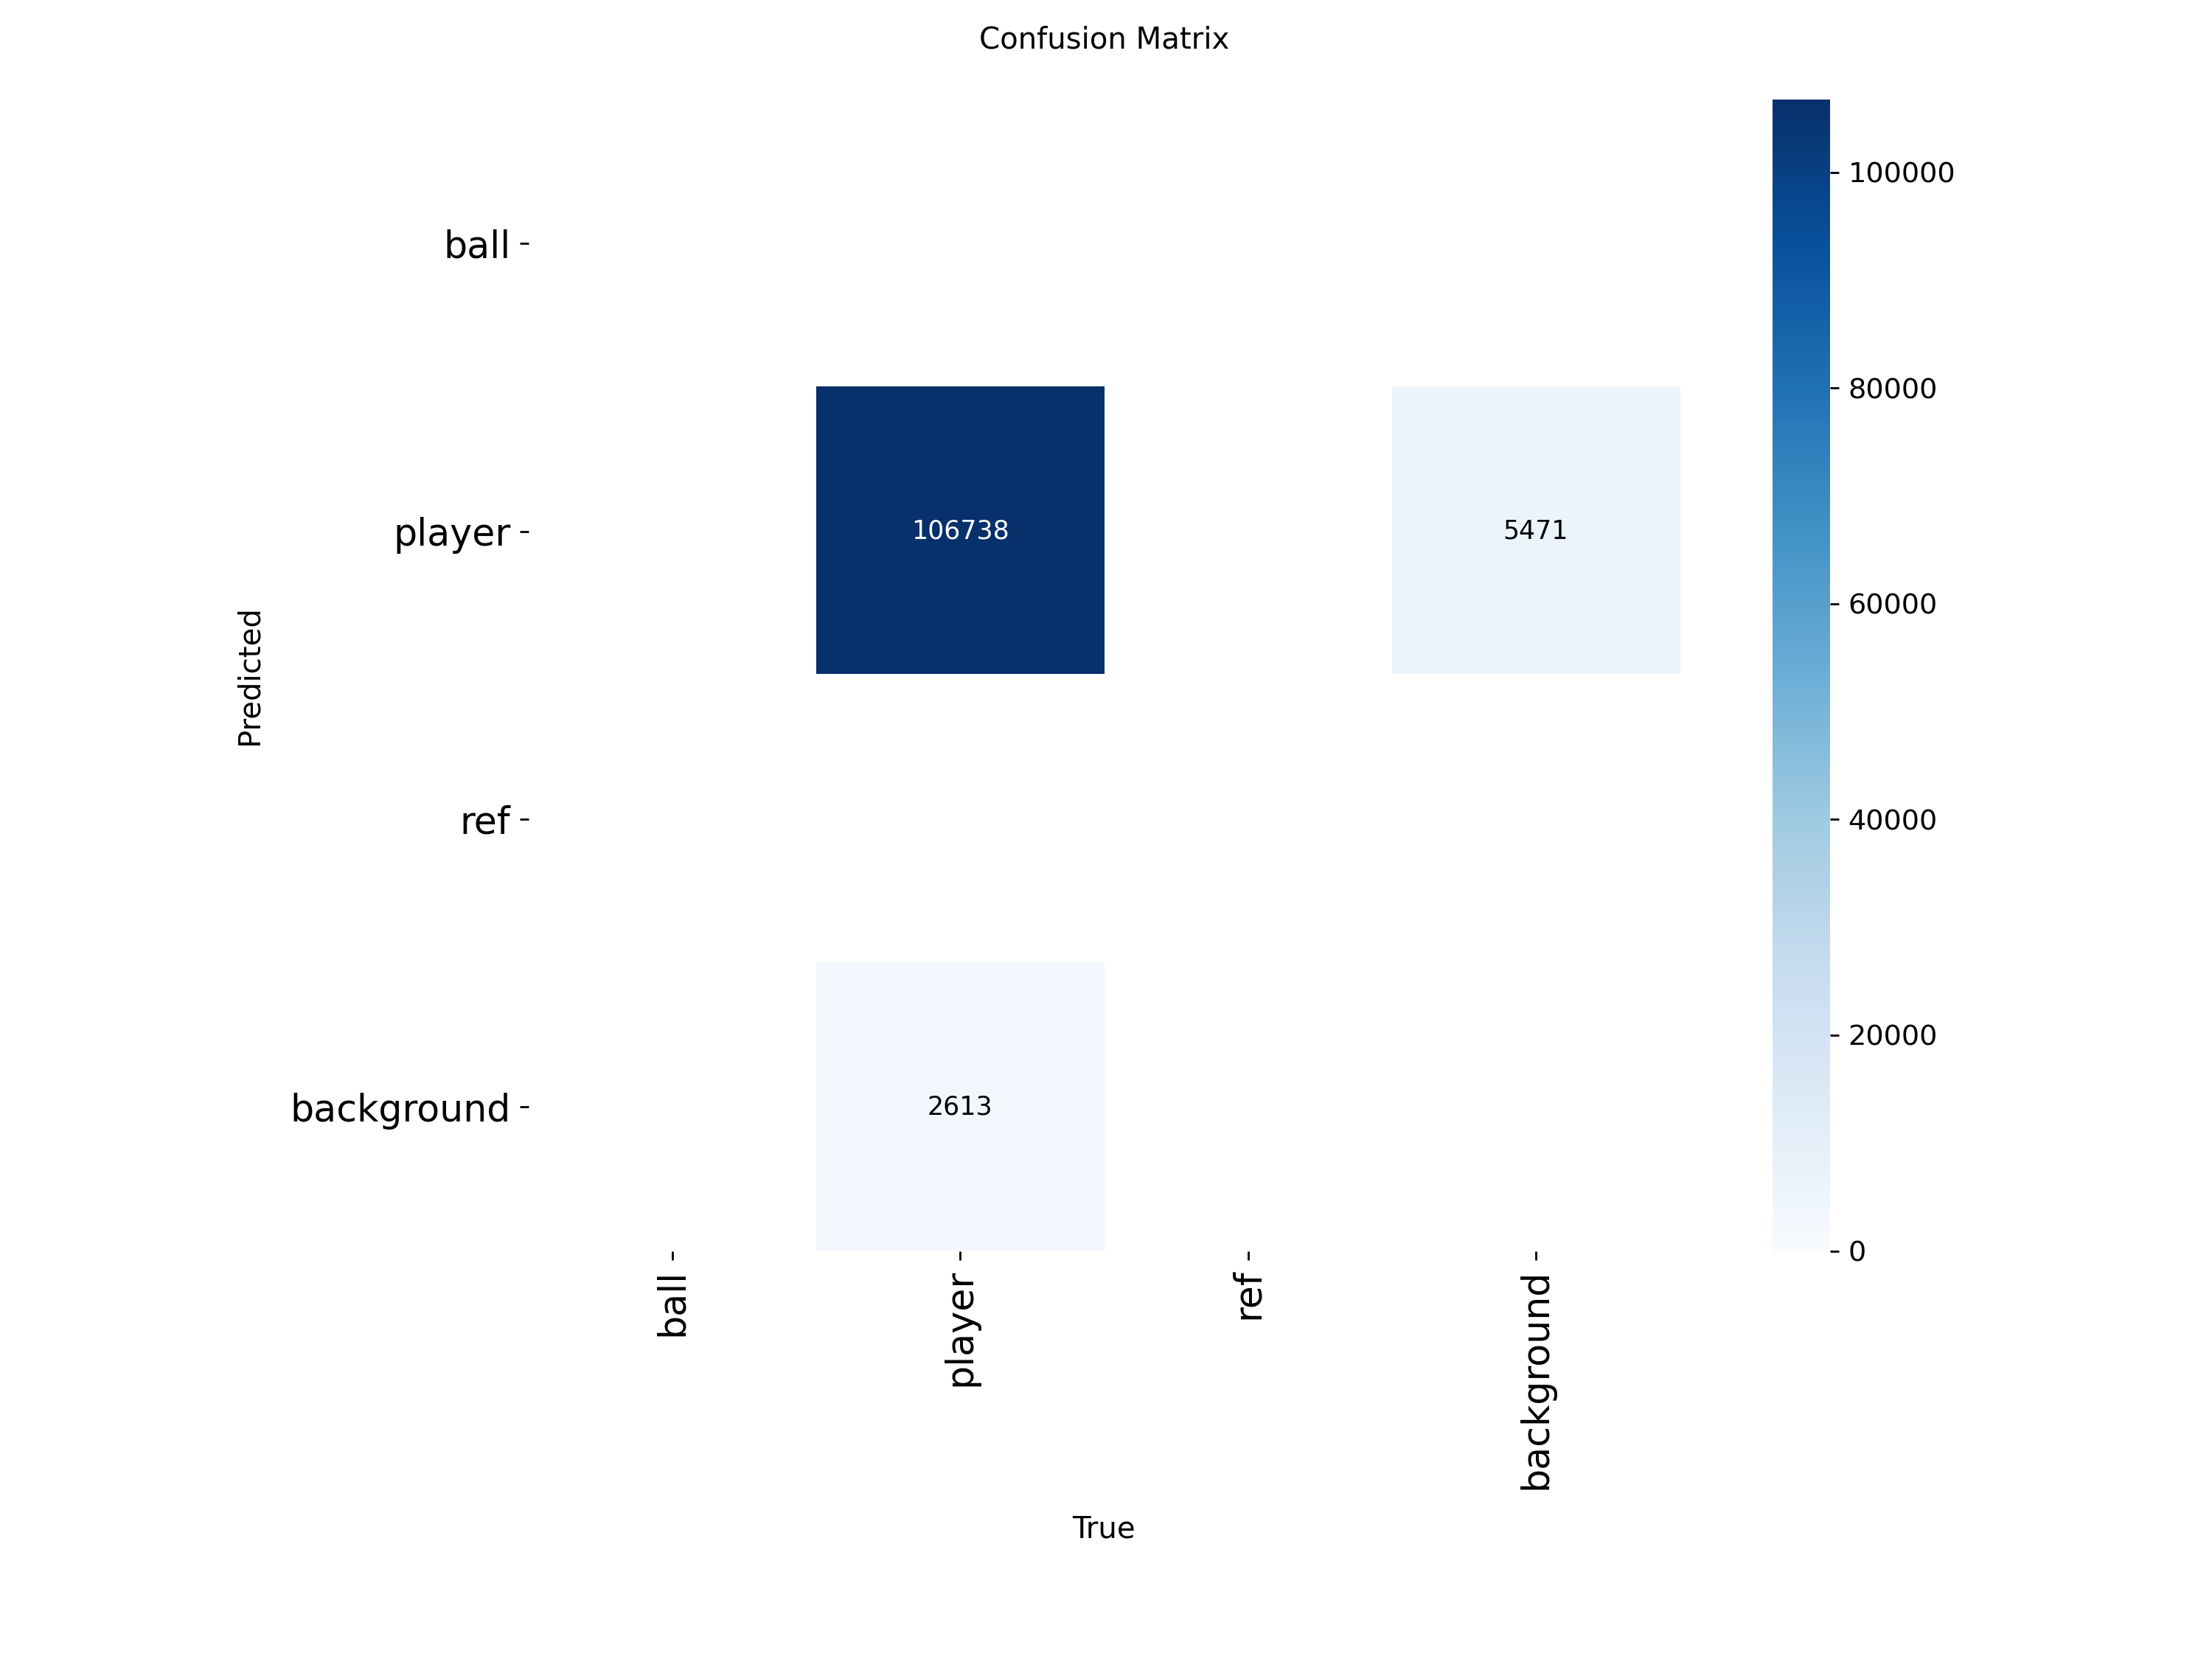
\includegraphics[width=\textwidth]{Imagenes/Propias/confusion_sinteticos.png}
    \small (a) Matriz de confusión en Datos Sintéticos
\end{minipage}

\vspace{0.4cm}

\begin{minipage}{0.55\textwidth}
    \centering
    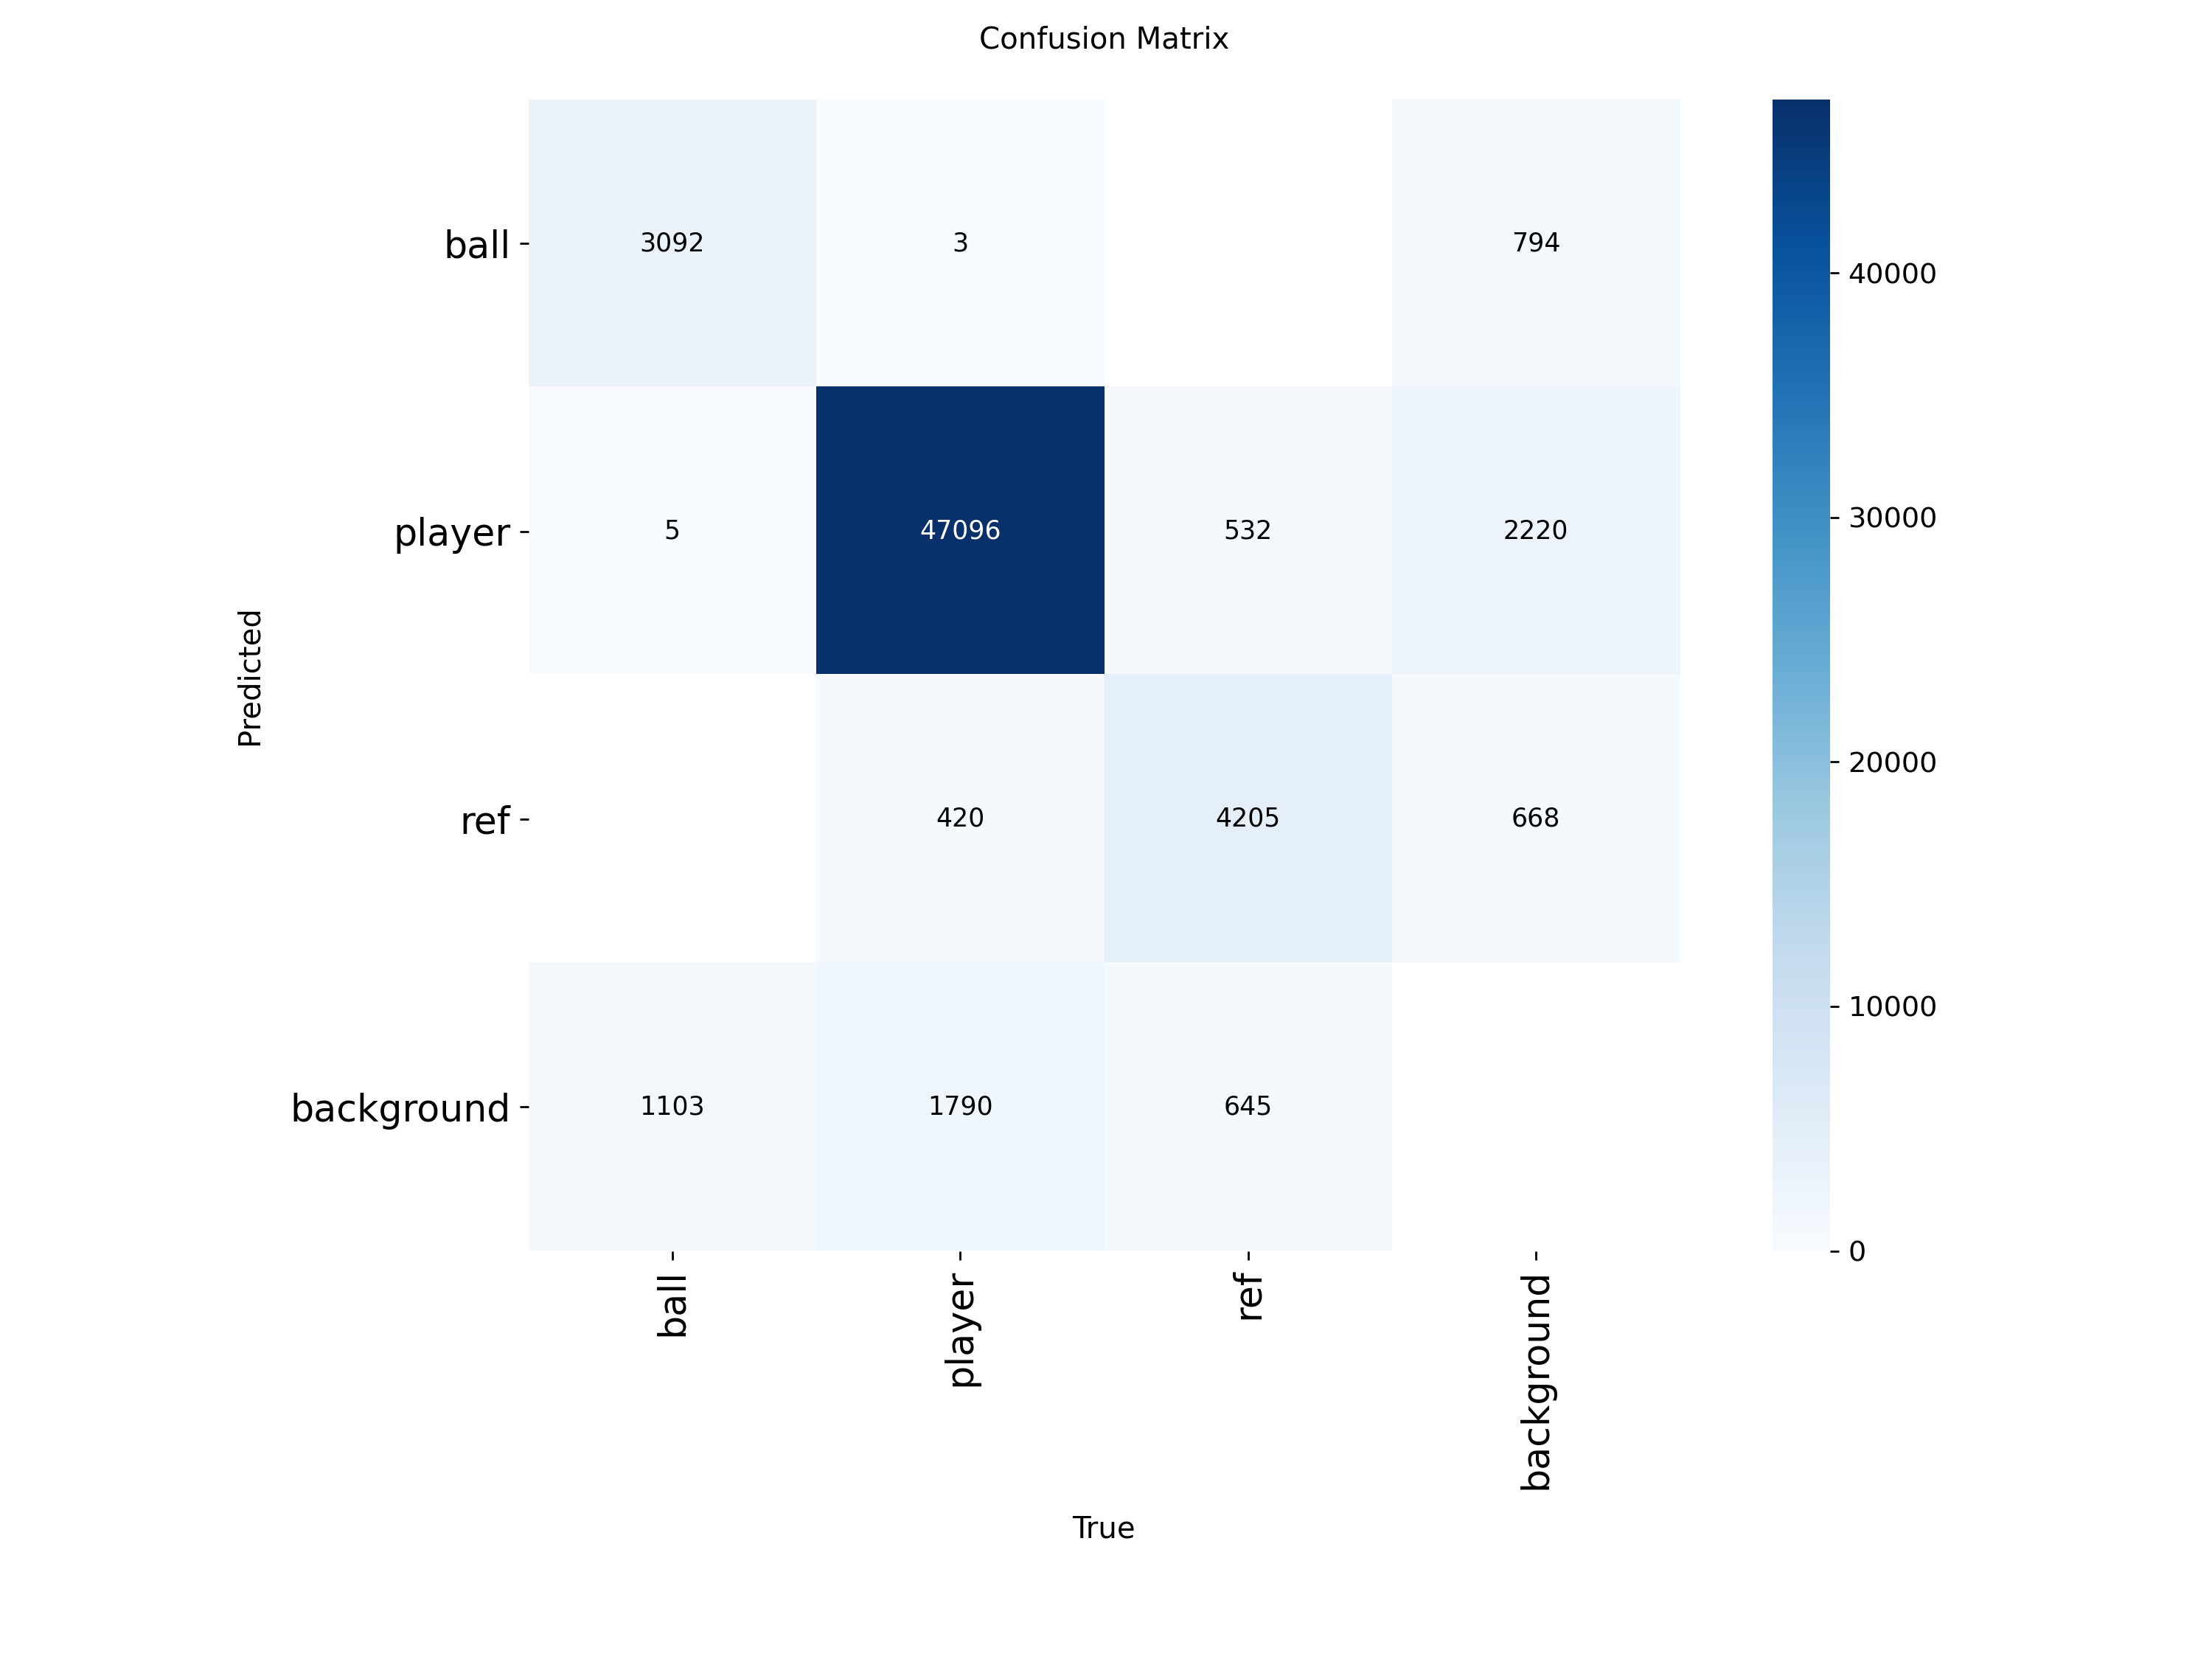
\includegraphics[width=\textwidth]{Imagenes/Propias/confusion_dfl.png}
    \small (b) Matriz de confusión en DFL-Bundesliga.
\end{minipage}

\caption[Matrices de confusión en los datasets de fine-tuning]{
Matrices de confusión en los datasets utilizados durante el \textit{fine-tuning} secuencial. La categoría \texttt{background} no corresponde a una clase entrenada del detector, sino que se incluye en la matriz para representar errores de detección, como objetos reales no detectados o predicciones que no se corresponden con ninguna anotación.
}


\label{fig:confusion_finetuning_compare}
\end{figure}

\subsection{Evaluación sobre la validación de DFL-Bundesliga}

Tras el entrenamiento, se realizó una comparación adicional entre los modelos sobre una misma partición de evaluación: el conjunto de validación de DFL-Bundesliga. El objetivo de esta prueba era comparar ambos detectores bajo un mismo dominio y con las mismas clases de evaluación. Aunque esta partición no se utilizó para actualizar los pesos durante el entrenamiento, no debe interpretarse como un conjunto externo completamente independiente, ya que pertenece al mismo dominio que la segunda fase del \textit{fine-tuning} secuencial.

\subsubsection{Modelos comparados}

En esta evaluación se compararon dos modelos. El primero corresponde al detector afinado directamente sobre el dataset Roboflow fútbol. El segundo corresponde al detector obtenido mediante el proceso secuencial de \textit{fine-tuning}, entrenado primero sobre SoccerSynth-Detection y refinado posteriormente sobre DFL-Bundesliga.

La evaluación se realizó sobre las clases comunes del conjunto de validación: \texttt{ball}, \texttt{player} y \texttt{ref}. La clase \texttt{goalkeeper}, presente en el modelo entrenado con Roboflow fútbol, no se evaluó como categoría independiente, sino que se mapeó a \texttt{player} para mantener una definición de clases común entre ambos modelos.


\subsubsection{Métricas utilizadas}

Las métricas de precisión, recall, F1 e IoU ya se definieron previamente en la \hyperref[subsec:metricas-deteccion-objetos]{Sección~\ref*{subsec:metricas-deteccion-objetos}}. En esta evaluación se utilizan para comparar el comportamiento de los dos detectores sobre la partición de validación de DFL-Bundesliga.

En primer lugar, se analiza el número de instancias reales frente al número de predicciones generadas por cada modelo, como se recoge en la \hyperref[tab:model_comparison_counts]{Tabla~\ref*{tab:model_comparison_counts}}. El número de instancias reales se indica como GT, mientras que el número de predicciones muestra cuántas detecciones produjo cada detector para cada clase. A partir de ambos valores se calcula la tasa de detección, definida como el cociente entre predicciones e instancias reales. Un valor inferior a 1 indica que el modelo tiende a detectar menos objetos de los anotados, mientras que un valor superior a 1 puede indicar mayor cobertura, aunque también riesgo de sobredetección.

La evaluación principal se realiza con un criterio estricto de IoU $\geq 0.50$. Bajo este criterio, una predicción se considera correcta únicamente si la clase coincide con la anotación real y el solape entre ambas cajas supera dicho umbral. A partir de esta correspondencia se calculan precisión, recall y F1 para cada clase, cuyos resultados se muestran en la \hyperref[tab:model_comparison_iou50]{Tabla~\ref*{tab:model_comparison_iou50}}.

Además, se calculan métricas más laxas para analizar la localización aproximada de los objetos, recogidas en la \hyperref[tab:model_comparison_soft]{Tabla~\ref*{tab:model_comparison_soft}}. El recall con IoU $\geq 0.10$ permite comprobar si el modelo detecta el objeto en una zona cercana aunque la caja no encaje con precisión. Esta métrica es útil en fútbol porque algunos objetos, especialmente el balón, pueden detectarse en la zona correcta pero con cajas poco estables. También se incluye un recall basado en centro, que considera correcta una detección si el centro de la caja real cae dentro de alguna caja predicha de la misma clase. Por último, la confianza media resume la seguridad promedio con la que cada modelo emite sus predicciones.


\subsection{Resultados cuantitativos}

La \hyperref[tab:model_comparison_counts]{Tabla~\ref*{tab:model_comparison_counts}} recoge el número de instancias reales y predicciones de cada modelo. La \hyperref[tab:model_comparison_iou50]{Tabla~\ref*{tab:model_comparison_iou50}} muestra la evaluación estricta con IoU $\geq 0.50$, mientras que la \hyperref[tab:model_comparison_soft]{Tabla~\ref*{tab:model_comparison_soft}} incluye métricas más laxas para analizar la localización aproximada de los objetos.

\begin{table}[H]
\centering
\scriptsize
\begin{tabular}{c|c|c|c|c|c}
\textbf{Clase} & \textbf{GT} & \textbf{Pred. Rob.} & \textbf{Pred. Sec.} & \textbf{Tasa Rob.} & \textbf{Tasa Sec.} \\
\hline\hline
\texttt{ball} & 4200 & 1650 & 5111 & 0.3929 & 1.2169 \\
\hline
\texttt{player} & 49570 & 53541 & 51812 & 1.0801 & 1.0452 \\
\hline
\texttt{ref} & 5382 & 5357 & 5503 & 0.9954 & 1.0225 \\
\hline
\end{tabular}
\caption[Instancias y predicciones en la validación de DFL-Bundesliga]{
Número de instancias reales, predicciones y tasa de detección de ambos modelos sobre la partición de validación de DFL-Bundesliga.
}
\label{tab:model_comparison_counts}
\end{table}

\begin{table}[H]
\centering
\scriptsize
\begin{tabular}{c|c|c|c|c|c|c}
\textbf{Clase} & \textbf{Prec. Rob.} & \textbf{Prec. Sec.} & \textbf{Recall Rob.} & \textbf{Recall Sec.} & \textbf{F1 Rob.} & \textbf{F1 Sec.} \\
\hline\hline
\texttt{ball} & 0.6582 & 0.6312 & 0.2586 & 0.7681 & 0.3713 & 0.6929 \\
\hline
\texttt{player} & 0.8642 & 0.9217 & 0.9335 & 0.9633 & 0.8975 & 0.9420 \\
\hline
\texttt{ref} & 0.7000 & 0.8390 & 0.6968 & 0.8579 & 0.6984 & 0.8483 \\
\hline
\end{tabular}
\caption[Comparación estricta con IoU $\geq 0.50$]{
Comparación estricta con IoU $\geq 0.50$ entre el modelo Roboflow y el modelo secuencial SoccerSynth+DFL.
}
\label{tab:model_comparison_iou50}
\end{table}

\begin{table}[H]
\centering
\scriptsize
\renewcommand{\arraystretch}{1.15}
\begin{tabular}{c|c|c|c|c|c|c}
\textbf{Clase} & \textbf{R@0.10 Rob.} & \textbf{R@0.10 Sec.} & \textbf{Centro Rob.} & \textbf{Centro Sec.} & \textbf{Conf. Rob.} & \textbf{Conf. Sec.} \\
\hline\hline
\texttt{ball} & 0.3114 & 0.8340 & 0.3129 & 0.8357 & 0.3522 & 0.5078 \\
\hline
\texttt{player} & 0.9427 & 0.9664 & 0.9743 & 0.9871 & 0.7394 & 0.7942 \\
\hline
\texttt{ref} & 0.7150 & 0.8610 & 0.7179 & 0.8634 & 0.6122 & 0.6951 \\
\hline
\end{tabular}
\caption[Métricas laxas en la validación de DFL-Bundesliga]{
Métricas laxas y confianza media de ambos modelos sobre la partición de validación de DFL-Bundesliga. R@0.10 indica recall con IoU $\geq 0.10$, Centro indica recall basado en centro, Rob. corresponde al modelo entrenado sobre Roboflow fútbol y Sec. al modelo secuencial SoccerSynth+DFL.
}
\label{tab:model_comparison_soft}
\end{table}

\subsection{Interpretación de los Resultados}
Los resultados muestran una mejora clara del modelo secuencial SoccerSynth+DFL sobre la partición de validación de DFL-Bundesliga. La diferencia es especialmente notable en la clase \texttt{ball}: el modelo Roboflow detecta 1650 balones frente a 4200 instancias reales, con un recall estricto de 0.2586, mientras que el modelo secuencial produce 5111 predicciones y alcanza un recall estricto de 0.7681. Aunque su precisión en balón es ligeramente menor, el aumento de cobertura resulta muy relevante para el sistema, ya que el balón es uno de los objetos más pequeños y difíciles de detectar.

En la clase \texttt{player}, el modelo secuencial también mejora las métricas principales, pasando de un F1 de 0.8975 a 0.9420. En la clase \texttt{ref}, la mejora es igualmente consistente, con un aumento del F1 de 0.6984 a 0.8483. Además, las métricas laxas muestran que el modelo secuencial localiza mejor los objetos incluso cuando se relaja el criterio de solape, lo que sugiere una mayor robustez espacial en este dominio.

Estos resultados indican que la estrategia de adaptación con datos sintéticos seguida de refinamiento sobre DFL-Bundesliga es más adecuada para este escenario que el entrenamiento directo sobre el dataset pequeño de Roboflow. No obstante, esta comparación debe interpretarse teniendo en cuenta que se realiza sobre la partición de validación de DFL-Bundesliga, por lo que no constituye una evaluación externa completamente independiente.

La decisión final del detector no debe basarse únicamente en estas métricas de detección aislada. El sistema completo depende también del comportamiento del tracking, de la estabilidad temporal de las identidades y de cómo se comporta el modelo sobre vídeos reales, donde aparecen compresión, movimiento de cámara, cambios de plano y oclusiones. Por este motivo, aunque esta comparación favorece al modelo sintético+DFL, la decisión final se deja abierta hasta completar las pruebas de tracking sobre vídeo real.
\section{Calibración del campo y proyección a coordenadas métricas}
\label{sec:calibracion-campo-proyeccion-metricas}

En la \hyperref[sec:homografia-tecnologias]{Sección~\ref*{sec:homografia-tecnologias}} se introdujo el concepto de homografía y se describió PnLCalib como método para estimar la calibración geométrica del campo en vídeo broadcast. En esta sección se resume cómo se ha integrado dicha calibración dentro del sistema y, especialmente, qué estrategias de robustez han sido necesarias para poder usar la homografía como una señal fiable dentro del pipeline.

\subsection{Modelo utilizado y salida geométrica}

En este proyecto se utiliza PnLCalib en modo inferencia, con sus pesos pre-entrenados publicados por los autores en el repositorio oficial del proyecto \citep{PnLCalibRepo2024}, para estimar en cada frame la geometría del campo visible. A partir de las predicciones de puntos y líneas del terreno se obtiene una homografía $H_t$ que permite proyectar coordenadas en píxeles $(u,v)$ a coordenadas 2D sobre el plano del campo $(x,y)$, expresadas en unidades métricas.

La \hyperref[fig:calibracion-proyeccion-campo]{Figura~\ref*{fig:calibracion-proyeccion-campo}} ilustra este proceso. En la imagen original se muestran los puntos de referencia detectados sobre el terreno de juego, mientras que la vista cenital resultante permite visualizar la proyección de la escena sobre el plano del campo.

\begin{figure}[H]
\centering

\begin{minipage}{0.9\textwidth}
    \centering
    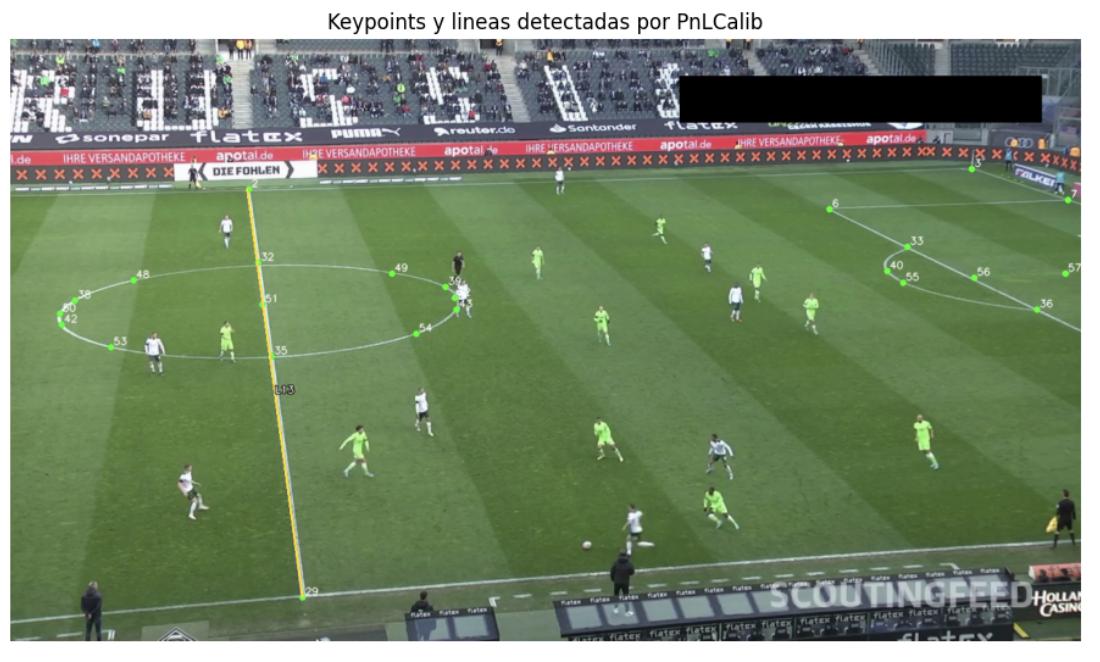
\includegraphics[width=\textwidth]{Imagenes/Propias/Puntos_referencia.png}
    \small \textbf{(a)} Puntos de referencia detectados sobre la imagen broadcast.
\end{minipage}

\vspace{0.4cm}

\begin{minipage}{0.9\textwidth}
    \centering
    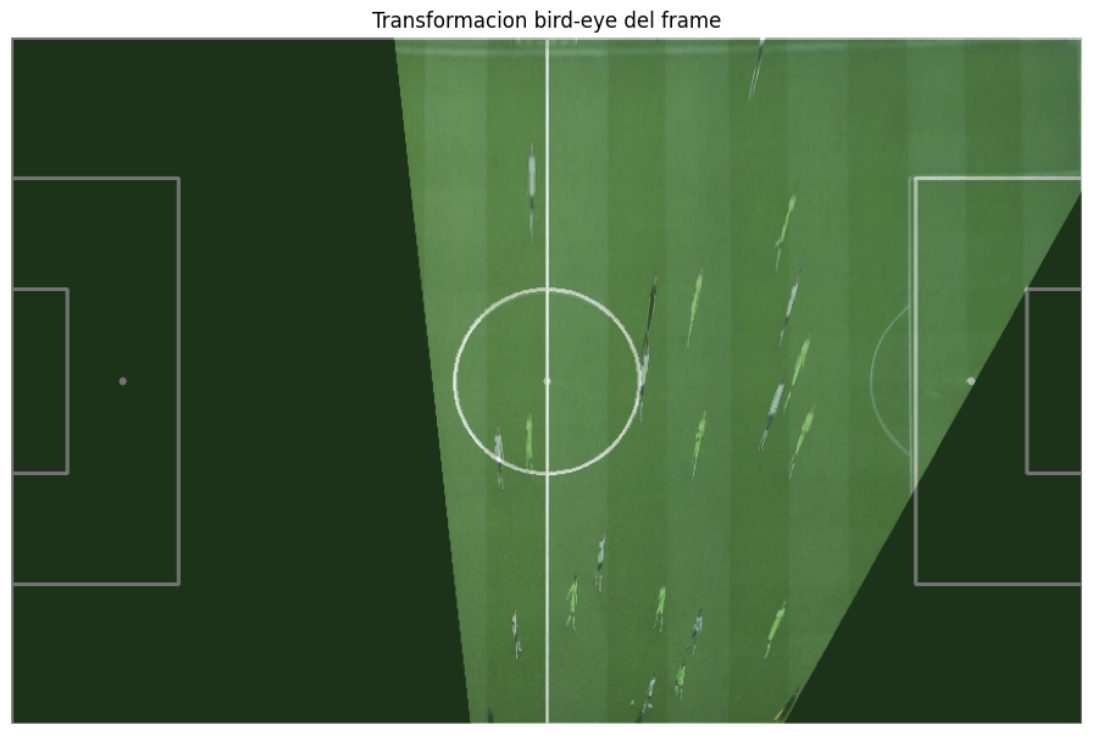
\includegraphics[width=\textwidth]{Imagenes/Propias/Bird_eye.png}
    \small \textbf{(b)} Proyección resultante en vista cenital del terreno de juego.
\end{minipage}

\caption[Calibración geométrica y proyección al plano del campo]{
Ejemplo de calibración geométrica del campo mediante PnLCalib. En (a) se muestran las referencias detectadas sobre la imagen broadcast y, en (b), la proyección de la escena sobre una representación 2D del terreno de juego.
}
\label{fig:calibracion-proyeccion-campo}
\end{figure}

Para proyectar la posición de un jugador no se utiliza el centro de su \textit{bounding box}, sino un punto que aproxima el contacto con el césped. En concreto, se emplea el punto central inferior de la caja, ligeramente desplazado hacia arriba:
\[
x = \frac{x_1 + x_2}{2}
\qquad
y = y_2 - 0.04 \cdot (y_2 - y_1)
\]
donde $(x_1,y_1,x_2,y_2)$ son las coordenadas de la \textit{bounding box}. Este punto se transforma mediante la homografía para obtener una posición $(x,y)$ en el campo.

La configuración de esta fase se resume en la \hyperref[tab:hiperparametros-referencia]{Tabla~\ref*{tab:hiperparametros-referencia}}, donde se recogen los parámetros utilizados por el módulo de proyección y sobre los que se irá hablando a lo largo de la sección.

\begin{table}[htbp]
\centering
\scriptsize
\setlength{\tabcolsep}{3pt}
\renewcommand{\arraystretch}{1.10}
\begin{tabularx}{\textwidth}{
>{\raggedright\arraybackslash}p{2.5cm}
>{\raggedright\arraybackslash}p{3.3cm}
>{\raggedright\arraybackslash}p{1.4cm}
>{\raggedright\arraybackslash}X
}
\toprule
\textbf{Bloque} & \textbf{Parámetro} & \textbf{Valor} & \textbf{Uso en pipeline} \\
\midrule

Redimensionado y punto de apoyo &
\texttt{bottom\_offset\_ratio} &
\texttt{0.04} &
Fija el desplazamiento vertical del punto proyectado sobre el césped. \\

\midrule

Umbrales base de inferencia &
\texttt{kp\_threshold} &
\texttt{0.30} &
Controla qué puntos de referencia se aceptan inicialmente. \\

&
\texttt{line\_threshold} &
\texttt{0.60} &
Controla qué líneas del campo se aceptan inicialmente. \\

&
\texttt{pnl\_refine} &
\texttt{false} &
Desactiva el refinamiento PnL adicional en esta configuración. \\

\midrule

Suavizado temporal &
\texttt{temporal\_blend} &
\texttt{0.20} &
Mezcla la homografía del frame actual con la anterior si la solución suavizada mantiene la calidad requerida. \\

\midrule

Búsqueda adaptativa &
\texttt{adaptive\_thresholds} &
\texttt{true} &
Activa varios intentos de calibración relajando umbrales. \\

&
\texttt{adaptive\_max\_attempts} &
\texttt{4} &
Número máximo de intentos por frame. \\

&
\texttt{adaptive\_kp\_step} &
\texttt{0.02} &
Reducción progresiva del umbral de puntos. \\

&
\texttt{adaptive\_line\_step} &
\texttt{0.05} &
Reducción progresiva del umbral de líneas. \\

&
\texttt{min. kp/line thresholds} &
\texttt{0.28/0.55} &
Límites inferiores hasta los que se relajan los umbrales. \\

\midrule

Soporte mínimo &
\texttt{min\_visible\_kp} &
\texttt{7} &
Número mínimo de puntos visibles requerido para aceptar una calibración. \\

&
\texttt{min\_visible\_lines} &
\texttt{1} &
Número mínimo de líneas visibles requerido para aceptar una calibración. \\

\midrule

Validación global &
\texttt{val\_score\_th} &
\texttt{0.56} &
Umbral mínimo del score compuesto de validación. \\

&
\texttt{val\_geometry\_fit\_min} &
\texttt{0.38} &
Mínimo requerido para la calidad del ajuste geométrico. \\

&
\texttt{val\_support\_quality\_min} &
\texttt{0.31} &
Mínimo requerido para la calidad del soporte geométrico. \\

&
\texttt{val\_coverage\_quality\_min} &
\texttt{0.18} &
Mínimo requerido para la cobertura de referencias. \\

\midrule

Validación geométrica &
\texttt{val\_reproj\_err\_px} &
\texttt{8.0} &
Rechaza soluciones con error de reproyección elevado. \\

&
\texttt{val\_H\_cond\_th} &
\texttt{1e8} &
Descarta homografías mal condicionadas. \\

&
\texttt{val\_kp\_world\_err\_m} &
\texttt{3.0} &
Limita el error métrico permitido en puntos. \\

&
\texttt{val\_line\_world\_err\_m} &
\texttt{4.0} &
Limita el error métrico permitido en líneas. \\

\midrule

Objetivos de cobertura &
\texttt{val\_target\_visible\_kp} &
\texttt{9} &
Objetivo de puntos visibles para considerar una calibración estable. \\

&
\texttt{val\_target\_visible\_lines} &
\texttt{4} &
Objetivo de líneas visibles. \\

&
\texttt{val\_target\_hull\_area} &
\texttt{0.18} &
Mide la cobertura espacial de los puntos en la imagen. \\

&
\texttt{val\_target\_x\_span} &
\texttt{0.55} &
Mide la extensión horizontal de las referencias. \\

&
\texttt{val\_target\_y\_span} &
\texttt{0.40} &
Mide la extensión vertical de las referencias. \\

&
\texttt{val\_target\_field\_cov} &
\texttt{0.20} &
Mide si las referencias cubren suficiente campo para estimar una homografía estable. \\

\bottomrule
\end{tabularx}

\caption[Hiperparámetros de calibración y proyección métrica]{
Hiperparámetros principales de la fase de calibración geométrica y proyección a coordenadas métricas.}
\label{tab:hiperparametros-referencia}
\end{table}

El valor final de estos hiperparámetros recogidos en la tabla se decidió mediante depuración iterativa y pruebas visuales sobre el vídeo de referencia. Este proceso de depuración se describe en la \hyperref[sec:evaluacion-heuristica-depuracion]{Sección~\ref*{sec:evaluacion-heuristica-depuracion}}.

\subsection{Problema de estabilidad: \textit{jitter} y sensibilidad a umbrales}

Durante las primeras pruebas se observó que la homografía estimada frame a frame era una señal poco estable: pequeñas variaciones en los puntos/líneas detectados producían cambios apreciables en la proyección, generando \textit{jitter} (vibración) tanto en la reconstrucción del campo como en las trayectorias proyectadas de los jugadores.

Este comportamiento ocurría principalmente con planos cerrados (esquinas o área), cuando la cámara realiza paneos o zooms rápidos, etc. 

Además, el método depende de umbrales de confianza para decidir qué puntos y líneas se consideran observados. En la práctica, fijar estos umbrales de forma única para todos los vídeos resulta difícil: con umbrales altos se obtienen menos referencias y muchos frames quedan sin homografía, mientras que con umbrales bajos se aceptan referencias ruidosas que degradan la calibración. Por tanto, la elección de umbrales tiene un componente arbitrario y el ``mejor'' valor depende del vídeo (calidad, resolución, iluminación y tipo de plano).

\subsection{Selección robusta de homografía: umbrales adaptativos y validación}

Para mejorar la robustez, se implementó una búsqueda por intentos con umbrales adaptativos sobre puntos clave y líneas. En cada frame se parte de una configuración base y se generan varios intentos relajando progresivamente los umbrales (hasta mínimos definidos), con el objetivo de aumentar el soporte geométrico en escenas difíciles.

El sistema evalúa todos los intentos y selecciona el mejor según un criterio lexicográfico: (i) aceptación de calidad, (ii) \textit{quality score} global y, en caso de empate, (iii) submétricas de ajuste geométrico, soporte y cobertura. Si ningún intento resulta aceptable, el frame se marca como no proyectable.

Esta estrategia permite adaptarse a distintos tipos de plano dentro del mismo partido (por ejemplo, plano general frente a plano cercano), y reduce la necesidad de calibrar manualmente umbrales por vídeo.

\subsubsection{Métricas de calidad y criterio de aceptación}

La homografía estimada no se utiliza de forma incondicional: se valida su calidad antes de habilitar su uso en tracking. El criterio que define la calidad de una homografía viene dado por la combinación de tres señales en un \textit{score} compuesto:
\begin{itemize}
    \item \textbf{Ajuste geométrico (\textit{geometry fit}):} incluye error de reproyección y chequeos de consistencia geométrica.
    \item \textbf{Soporte de referencias (\textit{support quality}):} cantidad y fiabilidad de puntos/líneas detectados.
    \item \textbf{Cobertura (\textit{coverage quality}):} distribución espacial/semántica de referencias para evitar soluciones concentradas o débiles.
\end{itemize}

Además del \textit{score} global, se aplican umbrales mínimos por submétrica y checks numéricos. Solo si el intento supera estos criterios se marca como aceptable para uso en tracking.

\subsubsection{Definición matemática de las métricas de calidad}

Sea un intento de calibración en un frame dado. Definimos funciones de normalización:
\[
clip(x)=\min(1,\max(0,x)),
\qquad
s_{\text{inv}}(e;\tau)=\frac{\tau}{\tau+e}
\]
\[
s_{\text{range}}(v;v_{\min},v_{\text{obj}})=
\mathrm{clip}\!\left(\frac{v-v_{\min}}{v_{\text{obj}}-v_{\min}}\right)
\]

Aquí, \({clip}\) acota cualquier valor al intervalo \([0,1]\), 
\(s_{\text{inv}}\) transforma un error \(e\) en una puntuación donde un valor mayor indica mejor calidad, y \(\tau\) controla la sensibilidad de esa transformación (en particular, \(s_{\text{inv}}=0.5\) cuando \(e=\tau\)), y \(s_{\text{range}}\) normaliza una magnitud \(v\) entre un mínimo y un objetivo, saturando el resultado en \([0,1]\).


Todas las submétricas se llevan a \([0,1]\), donde \(1\) es mejor.

\paragraph{1) Ajuste geométrico}
\[
G = 0.35\,s_{\text{rep}} + 0.15\,s_{\text{cond}} + 0.30\,s_{\text{kp-align}} + 0.20\,s_{\text{line-align}}
\]
con:
\[
s_{\text{rep}} = s_{\text{inv}}(e_{\text{rep}};\tau_{\text{rep}}),
\qquad
s_{\text{cond}}=
\mathrm{clip}\!\left(
1-\frac{\log_{10}(\kappa(H))}{\log_{10}(\kappa_{\max})}
\right),
\]
\[
s_{\text{kp-align}} = s_{\text{inv}}(e_{\text{kp-world}};\tau_{\text{kp-world}}),
\qquad
s_{\text{line-align}} = s_{\text{inv}}(e_{\text{line-world}};\tau_{\text{line-world}}).
\]

Donde \(e_{\text{rep}}\) es el error de reproyección devuelto por PnLCalib, \(\kappa(H)\) es el número de condición de la homografía \(H\), y \(e_{\text{kp-world}}\), \(e_{\text{line-world}}\) son errores medianos en metros tras proyectar puntos y líneas al campo. Los umbrales \(\tau_{\text{rep}}\), \(\kappa_{\max}\), \(\tau_{\text{kp-world}}\) y \(\tau_{\text{line-world}}\) corresponden a los valores de la Tabla~\ref{tab:hiperparametros-referencia} (respectivamente: \textit{val\_reproj\_err\_px}, \textit{val\_H\_cond\_th}, \textit{val\_kp\_world\_err\_m}, \textit{val\_line\_world\_err\_m}).

\(s_{\text{rep}}\) mide la consistencia global de la proyección en imagen (qué bien se reinyectan las referencias detectadas), \(s_{\text{cond}}\) mide la estabilidad numérica de la homografía estimada penalizando matrices mal condicionadas, \(s_{\text{kp-align}}\) mide la coherencia métrica de los puntos clave proyectados sobre el campo, y \(s_{\text{line-align}}\) mide la coherencia métrica de las líneas proyectadas en el plano del campo. En conjunto, estas submétricas capturan tanto el ajuste visual en imagen como la validez geométrica y la estabilidad numérica de la solución en coordenadas de juego.


\paragraph{2) Calidad del soporte de las referencias}
\[
S =
0.25\,s_{\text{kp-count}}
+ 0.20\,s_{\text{line-count}}
+ 0.15\,s_{\text{kp-conf}}
+ 0.10\,s_{\text{line-conf}}
+ 0.15\,s_{\text{kp-family}}
+ 0.15\,s_{\text{line-family}}.
\]

con:
\[
s_{\text{kp-count}}=
s_{\text{range}}(N_{kp};N_{kp}^{\min},N_{kp}^{obj}),\qquad
s_{\text{line-count}}=
s_{\text{range}}(N_{line};N_{line}^{\min},N_{line}^{obj}),
\]
\[
s_{\text{kp-conf}}=\frac{1}{N_{kp}}\sum_{i=1}^{N_{kp}} c^{kp}_i,\qquad
s_{\text{line-conf}}=\frac{1}{N_{line}}\sum_{j=1}^{N_{line}} c^{line}_j,
\]
\[
s_{\text{kp-family}}
=
\frac{1}{2}\left(\frac{B_x}{3}+\frac{B_y}{3}\right),
\]
\[
s_{\text{line-family}}
=
\mathrm{clip}\!\left(\frac{F_{\text{line}}}{3}\right).
\]

Donde \(N_{kp}\) y \(N_{line}\) son el número de \textit{keypoints} y líneas visibles; \(c^{kp}_i\) y \(c^{line}_j\) son sus confianzas individuales (devueltas por PnLCalib); \(B_x\) y \(B_y\) son el número de bandas ocupadas por los \textit{keypoints} en los ejes longitudinal y transversal del campo, tras dividir cada eje en tres intervalos; y \(F_{\text{line}}\) es el número de familias geométricas de líneas observadas, distinguiendo entre horizontales, verticales y estructura de portería.

Los umbrales y objetivos \(N_{kp}^{\min}\), \(N_{line}^{\min}\), \(N_{kp}^{obj}\) y \(N_{line}^{obj}\) corresponden a los valores de la Tabla~\ref{tab:hiperparametros-referencia} (respectivamente: \textit{min\_visible\_kp}, \textit{min\_visible\_lines}, \textit{val\_target\_visible\_kp}, \textit{val\_target\_visible\_lines}).

En esta puntuación, \(s_{\text{kp-count}}\) y \(s_{\text{line-count}}\) miden suficiencia de evidencia, \(s_{\text{kp-conf}}\) y \(s_{\text{line-conf}}\) miden fiabilidad media de las detecciones, \(s_{\text{kp-family}}\) mide si los \textit{keypoints} cubren zonas distintas del campo, y \(s_{\text{line-family}}\) mide si las líneas observadas pertenecen a familias geométricas variadas. En conjunto, estas submétricas intentan captar si la calibración se apoya en referencias no solo numerosas y fiables, sino también diversas.

\paragraph{3) Calidad de la cobertura del campo}
\[
C = 0.40\,s_{\text{img-hull}} + 0.20\,s_{\text{field-hull}} + 0.20\,s_{x\text{-span}} + 0.20\,s_{y\text{-span}}
\]
con:
\[
s_{\text{img-hull}}=\mathrm{clip}\!\left(\frac{A_{\text{img-hull}}}{A_{\text{img-hull}}^{\text{obj}}}\right),\qquad
s_{\text{field-hull}}=\mathrm{clip}\!\left(\frac{A_{\text{field-hull}}}{A_{\text{field-hull}}^{\text{obj}}}\right),
\]
\[
s_{x\text{-span}}=\mathrm{clip}\!\left(\frac{p_{x\text{-span}}}{p_{x\text{-span}}^{\text{obj}}}\right),\qquad
s_{y\text{-span}}=\mathrm{clip}\!\left(\frac{p_{y\text{-span}}}{p_{y\text{-span}}^{\text{obj}}}\right).
\]

Donde \(A_{\text{img-hull}}\) es la fracción de área del casco convexo de las referencias en imagen respecto al área total del frame; \(A_{\text{field-hull}}\) es la fracción de área del casco convexo de las referencias proyectadas en el campo respecto al área total del terreno de juego; y \(p_{x\text{-span}}\), \(p_{y\text{-span}}\) son las fracciones del ancho y del alto de la imagen cubiertas por la separación entre la referencia más extrema a izquierda/derecha y la más extrema arriba/abajo, respectivamente.

Los objetivos \(A_{\text{img-hull}}^{\text{obj}}\), \(A_{\text{field-hull}}^{\text{obj}}\), \(p_{x\text{-span}}^{\text{obj}}\) y \(p_{y\text{-span}}^{\text{obj}}\) corresponden a los valores de la Tabla~\ref{tab:hiperparametros-referencia} (respectivamente: \textit{val\_target\_hull\_area}, \textit{val\_target\_field\_cov}, \textit{val\_target\_} \textit{x\_span}, \textit{val\_target\_y\_span}).

En esta puntuación, \(s_{\text{img-hull}}\) mide cuánta superficie útil del frame queda anclada por referencias, \(s_{\text{field-hull}}\) mide su cobertura geométrica tras proyectarlas al plano del campo, y \(s_{x\text{-span}}\), \(s_{y\text{-span}}\) miden cuánto se extienden dichas referencias a lo ancho y a lo alto de la imagen. En conjunto, estas submétricas evalúan si la calibración está soportada por una cobertura amplia y bien distribuida.

\paragraph{Score final y criterio de aceptación:}

Si existe una homografía candidata válida, se calcula una puntuación global como combinación ponderada de las tres métricas anteriores:
\[
Q = 0.45\,G + 0.30\,S + 0.25\,C.
\]

Los umbrales de aceptación sobre estas métricas vienen dados por:
\[
G \ge G_{\min},\quad S \ge S_{\min},\quad C \ge C_{\min},\quad Q \ge Q_{\min},
\]
donde \(G_{\min}\), \(S_{\min}\), \(C_{\min}\) y \(Q_{\min}\) corresponden a los valores de la Tabla~\ref{tab:hiperparametros-referencia} (respectivamente: \textit{val\_geometry\_fit\_min}, \textit{val\_support\_quality\_min}, \textit{val\_coverage\_quality\_min}, \textit{val\_score\_th}).

Sin embargo, la aceptación final no depende solo de estas puntuaciones agregadas. Además, se aplican comprobaciones duras de validez: debe existir una homografía estimada, esta debe ser numéricamente válida y estar suficientemente bien condicionada, y el frame debe alcanzar al menos los mínimos de referencias visibles \(N_{kp}^{\min}\) y \(N_{line}^{\min}\). Por tanto, una solución puede obtener valores altos de \(G\), \(S\), \(C\) y \(Q\), pero aun así ser rechazada si falla alguna de estas condiciones duras.

\subsection{Suavizado temporal}

Incluso con homografías aceptables, puede existir variación frame a frame. Para reducir vibraciones se aplica un suavizado temporal opcional:
\[
H_t^{blend}=\alpha H_{t-1} + (1-\alpha)H_t^{raw}, \quad \alpha=0.20
\]

En la implementación, el resultado suavizado se conserva únicamente si también supera la validación de calidad y no reduce el \textit{quality score} frente a la solución no suavizada.

\subsection{Fallo controlado: \textit{fallback} cuando no hay homografía}

Por último, cuando no se consigue una homografía fiable, el pipeline no se detiene: se descarta la proyección métrica en ese frame y las fases posteriores continúan trabajando en coordenadas de imagen. Esta decisión evita que una calibración errónea contamine el resto del sistema.

En la \hyperref[fig:homography_frame]{Figura~\ref*{fig:homography_frame}} se muestra un ejemplo visual de la salida de esta fase para un frame del vídeo de prueba. En el panel de la izquierda aparecen las detecciones, los puntos y las líneas de referencia encontrados. En el de la derecha se muestra cómo quedan ubicadas las detecciones sobre el campo tras aplicar la homografía. El vídeo del resultado completo puede consultarse en \url{https://github.com/hectorgarciaa/narrador-futbol/output/homography/best/20260516_180637/homography.mp4}.
\begin{figure}[h]
    \centering
    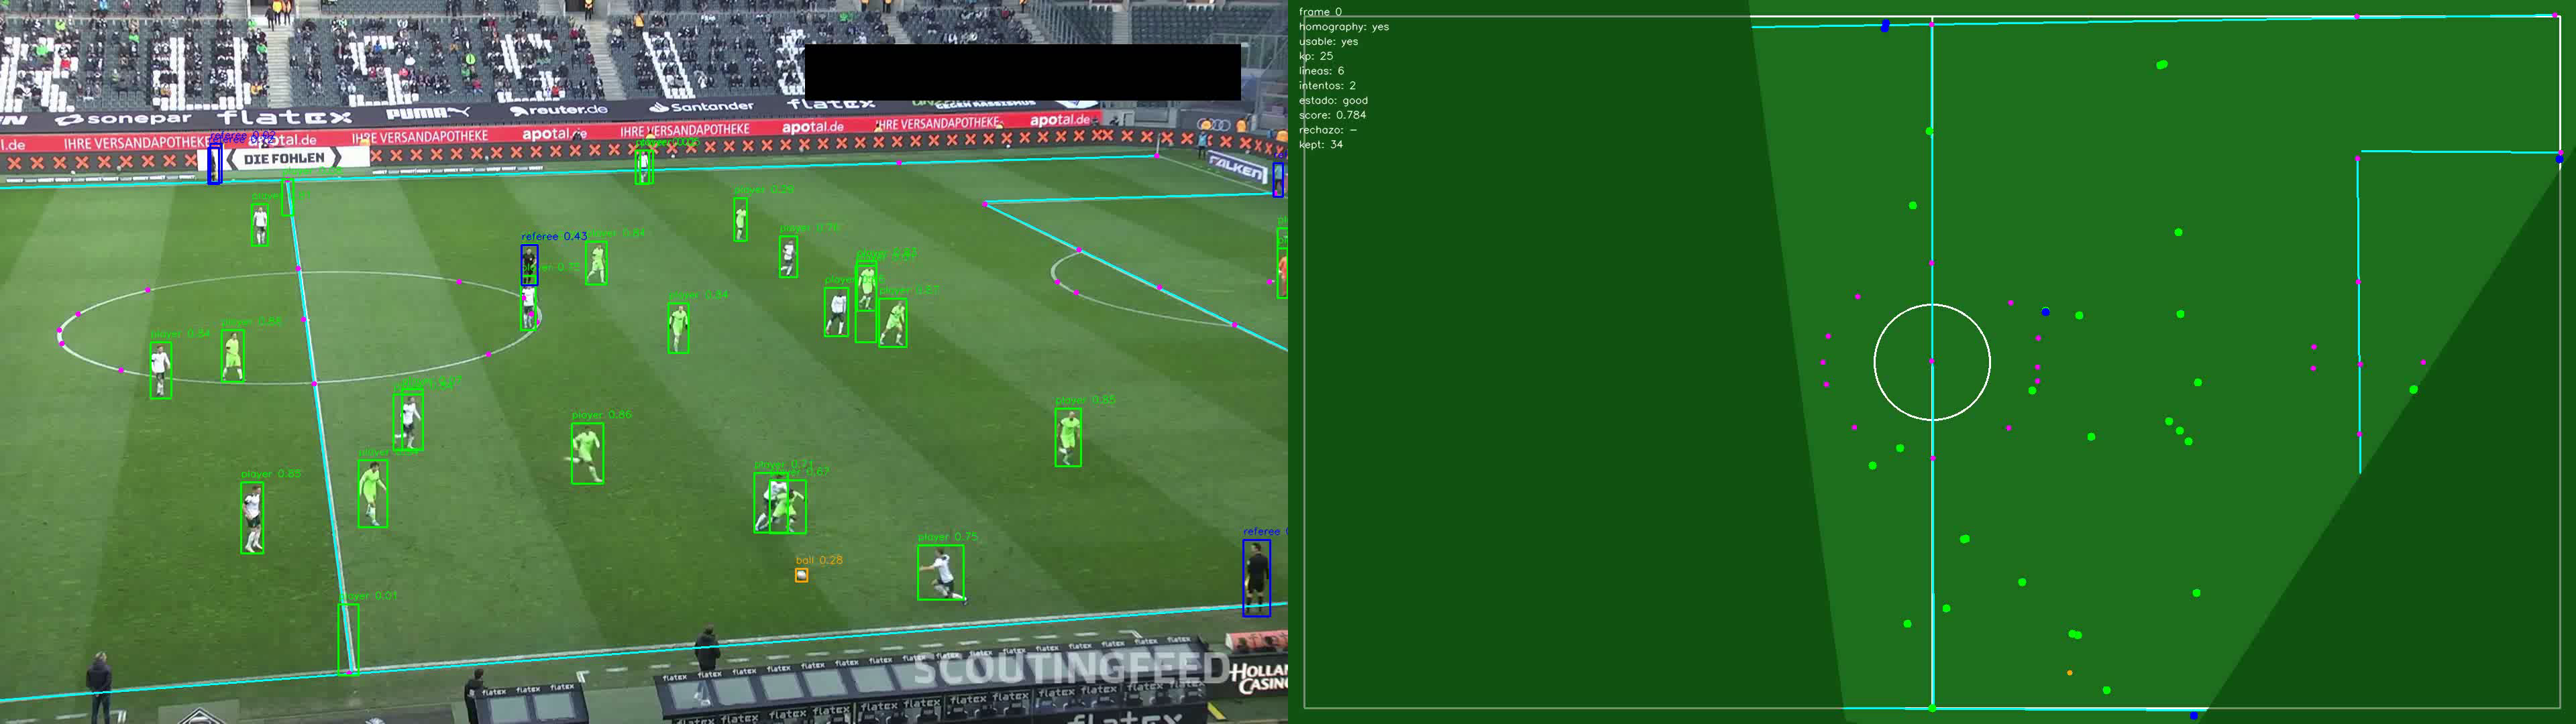
\includegraphics[width=0.85\textwidth]{Imagenes/Propias/homography_frame.png}
    \caption{Resultado visual de la fase de calibración del campo y proyección.}
    \label{fig:homography_frame}
\end{figure}

\section{Clasificación de equipos}

Tras la fase de calibración y proyección, el siguiente paso del pipeline consiste en identificar a qué equipo pertenece cada detección. El detector inicial permite diferenciar clases como jugador, portero, árbitro o balón, pero no proporciona directamente la pertenencia de equipo de cada futbolista. Para resolver esta limitación se implementa una fase específica de asignación basada en el color de la camiseta.

El planteamiento parte de una hipótesis sencilla: en un partido de fútbol, el rasgo visual más estable para distinguir a los jugadores de un equipo frente a los del rival es el color de la equipación. A partir de esta idea, la clasificación se divide en dos procesos: primero, la extracción del color representativo de la camiseta para cada detección candidata y después la asociación de ese color a uno de los dos equipos de campo presentes en el partido.

Todo este proceso se realiza en el espacio de color LAB. En este espacio, el canal $L$ representa la luminosidad, el canal $A$ codifica la oposición entre verde y rojo, y el canal $B$ codifica la oposición entre azul y amarillo. En la implementación de OpenCV estos valores se almacenan escalados en el rango $[0,255]$, con los canales $A$ y $B$ centrados aproximadamente en 128 para representar valores neutros. Se ha escogido LAB porque la distancia euclídea entre dos colores en este espacio se aproxima mejor a la diferencia perceptual que en RGB, lo que resulta útil para comparar colores de camisetas bajo distintas condiciones de iluminación. Aun así, este espacio no elimina por completo el efecto de sombras, reflejos o cambios de luz, especialmente porque el canal $L$ sigue dependiendo de la luminosidad de la imagen.

\subsection{Identificación del color de la camiseta}

La identificación del color de la camiseta parte de las cajas delimitadoras generadas por el detector. En la implementación se utilizan las coordenadas de la caja en formato $(x_1, y_1, x_2, y_2)$, que delimitan la región de la imagen donde se encuentra cada detección (jugador, portero o árbitro). Como la camiseta se encuentra normalmente en la parte superior del cuerpo, se recorta únicamente el 50\% superior del \textit{bounding box}. De esta forma se reduce la influencia del pantalón, las botas y parte del césped.

Esta aproximación no cubre todos los casos posibles. Por ejemplo, un jugador puede aparecer en el suelo, girado o parcialmente ocluido, pero estos casos son menos frecuentes y se asumen como excepciones dentro de un sistema que debe funcionar de forma robusta en la mayoría de frames.

Una vez extraída la región superior de la caja, todavía aparece un problema importante: el \textit{bounding box} es rectangular, mientras que el cuerpo del jugador no lo es. Por tanto, dentro del recorte no solo aparece la camiseta, sino también césped, cabeza, brazos u otros elementos de fondo. Para separar la camiseta del resto de píxeles se aplica KMeans con $k=2$ sobre los píxeles del recorte en espacio LAB. La idea es dividir los colores del recorte en dos grupos principales: uno correspondiente a la camiseta y otro correspondiente al fondo.

Aunque podrían plantearse más clusters, por ejemplo para separar cabeza, camiseta y césped, en la práctica $k=2$ ofrece un compromiso adecuado entre simplicidad, estabilidad y coste computacional. La cabeza o pequeñas regiones secundarias suelen quedar absorbidas por uno de los dos clusters, y su influencia sobre el centroide final es limitada si ocupan pocos píxeles frente a la camiseta o el fondo.

Para decidir qué cluster corresponde a la camiseta no se toma simplemente el cluster mayoritario, ya que en algunos recortes el fondo puede ocupar más superficie que el propio jugador. En su lugar, se selecciona un conjunto fijo de puntos de referencia del recorte (esquinas y bordes: superior-izquierda, superior-derecha, inferior-izquierda, inferior-derecha, centro superior, centro lateral izquierdo y centro lateral derecho). Estos puntos suelen pertenecer al fondo, por lo que el cluster más frecuente entre ellos se interpreta como fondo. El otro cluster se considera el de la camiseta, y su centroide LAB se guarda como color representativo de la detección.

\begin{equation}
\mathbf{c}_{\text{camiseta}} = [L, A, B]
\label{eq:color-camiseta-lab}
\end{equation}

Este proceso se aplica a cada detección (jugadores, árbitros y porteros). La decisión final de equipo y posibles reetiquetados de clase (por ejemplo, entre jugador, portero y árbitro) se realiza en la etapa de asociación descrita en el siguiente \hyperref[subsec:asociacionEquipo]{Apartado~\ref*{subsec:asociacionEquipo}}. En la \hyperref[fig:shirt-crop-kmeans]{Figura~\ref*{fig:shirt-crop-kmeans}} se muestra un ejemplo del recorte superior y la segmentación de color utilizada para estimar \(c_{camiseta}\).
\begin{figure}[H]
    \centering
    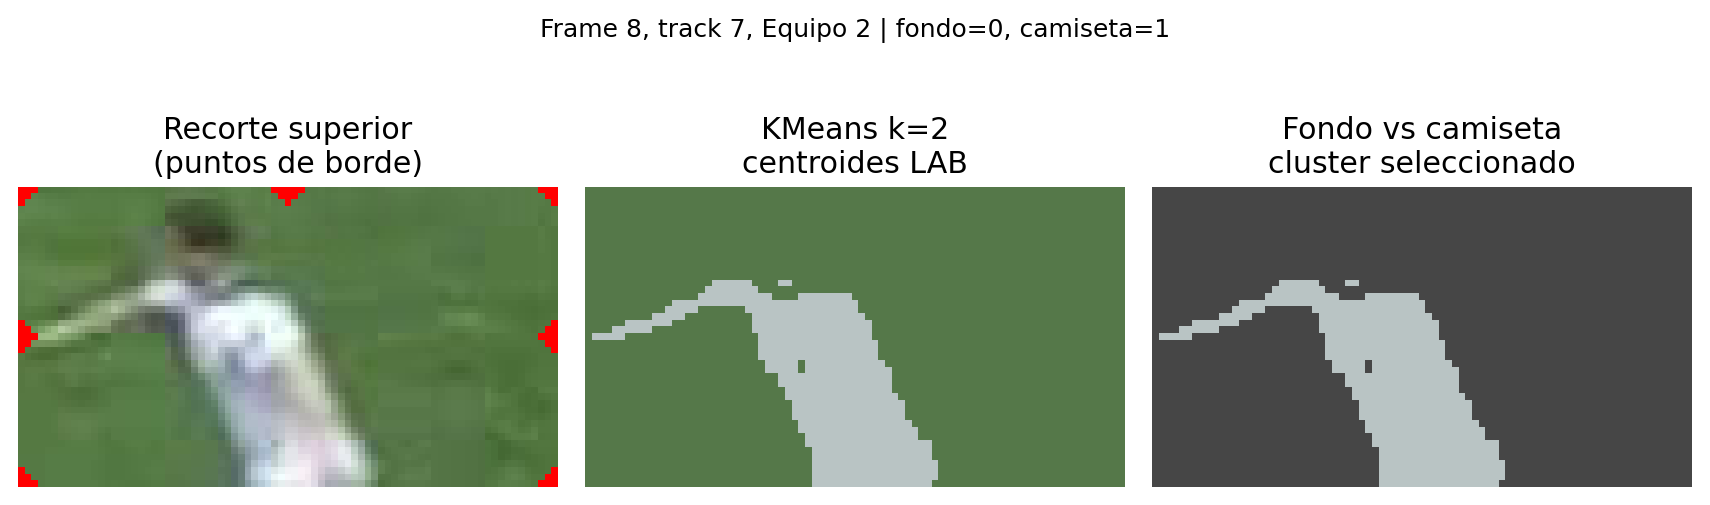
\includegraphics[width=0.9\textwidth]{Imagenes/Propias/shirt_crop_kmeans_example.png}
    \caption[Recorte de crop de jugador y KMeans]{Ejemplo de recorte superior de jugador y segmentación mediante KMeans con $k=2$.}
    \label{fig:shirt-crop-kmeans}
\end{figure}

\subsection{Asociación del equipo}
\label{subsec:asociacionEquipo}

En esta sección se describe la lógica para asociar cada track detectado a uno de los dos equipos.

\subsubsection{Asignación por color y centro del equipo}

Una vez obtenido el color de camiseta de cada detección candidata, representado por el vector $\mathbf{c}_{\text{camiseta}}$ definido en la Ecuación~\eqref{eq:color-camiseta-lab}, el objetivo es asociarlo a uno de los dos equipos de campo del partido. Para ello se acumulan muestras de colores LAB de las camistas de los jugadores y se aplica KMeans con $k=2$, esta vez no sobre píxeles individuales, sino sobre los colores de las camisetas ya extraídos. Cada cluster representa uno de los dos equipos de campo.

El centro de cada equipo se calcula mediante la mediana de las muestras LAB del cluster, en lugar de usar directamente la media. Esta decisión hace que la referencia de color sea más robusta frente a detecciones erróneas, sombras, reflejos o recortes en los que la camiseta no se haya aislado correctamente.

La asignación de una nueva detección se realiza calculando la distancia euclídea entre el color de su camiseta y el color de referencia de cada equipo:

\[
d(c, \mu_t) = \|c - \mu_t\|_2
\]

donde $c$ es el color LAB de la camiseta detectada y $\mu_t$ es el color representativo del equipo $t$. La detección se asigna al equipo cuya referencia esté más cerca:

\[
equipo(c) = \arg\min_t d(c, \mu_t)
\]


\subsubsection{Actualización online, \textit{bootstrap} y \textit{buckets} de muestras}

La construcción de clusters de color se realiza en modo online mediante un esquema de \textit{buckets} por clase, con dos contenedores principales: muestras de campo (\texttt{player}) y muestras de árbitro (\texttt{referee}). Cada nueva detección con color estimado solo se incorpora si supera una confianza mínima configurable.

Durante las primeras fases del vídeo, cuando los clusters de equipos todavía no están estabilizados, el sistema acumula muestras progresivamente y retrasa la actualización hasta disponer de soporte suficiente. Para el \textit{bucket} de jugadores, la actualización de centros no se lanza en cada frame, sino de forma periódica (cada 5 frames) y únicamente cuando se alcanza un mínimo de muestras acumuladas (en nuestra configuración, 60).

Cuando se ejecuta la actualización, se aplica KMeans con $k=2$ sobre las muestras LAB de jugadores. Después se valida el tamaño de los clusters obtenidos: si alguno resulta demasiado pequeño (por debajo de un mínimo configurable), se considera un cluster inválido, se descarta y se repite el ajuste sobre el cluster mayor. Si tras varias iteraciones no se obtiene una partición estable, la actualización se rechaza y se espera a nuevas muestras.

Además, para cada equipo se calculan estadísticas robustas de distancia intra-cluster (cuartiles e IQR), a partir de las cuales se define un umbral superior de pertenencia. Estas cotas se usan para detectar colores alejados del patrón esperado y limitar el impacto de \textit{outliers}.

En el caso del árbitro, el color de referencia no se estima con KMeans, sino mediante media recortada (\textit{trimmed mean}) sobre las muestras LAB acumuladas (recorte del 15\% por canal), lo que reduce la influencia de valores extremos y mejora la robustez del modelo.

En la \hyperref[fig:team-color-clusters-lab]{Figura~\ref*{fig:team-color-clusters-lab}} se puede ver como queda el estado de color de un partido después una ejecución. Se puede ver como el sistema es capaz de definir clusters bastante acertados sobre los colores de cada grupo de detecciones. Concretamente se puede ver el cluster del Equipo 1, de color verde, el cluster del Equipo 2, de color blanco, y el cluster de árbitros, de color negro. 

\begin{figure}[H]
    \centering
    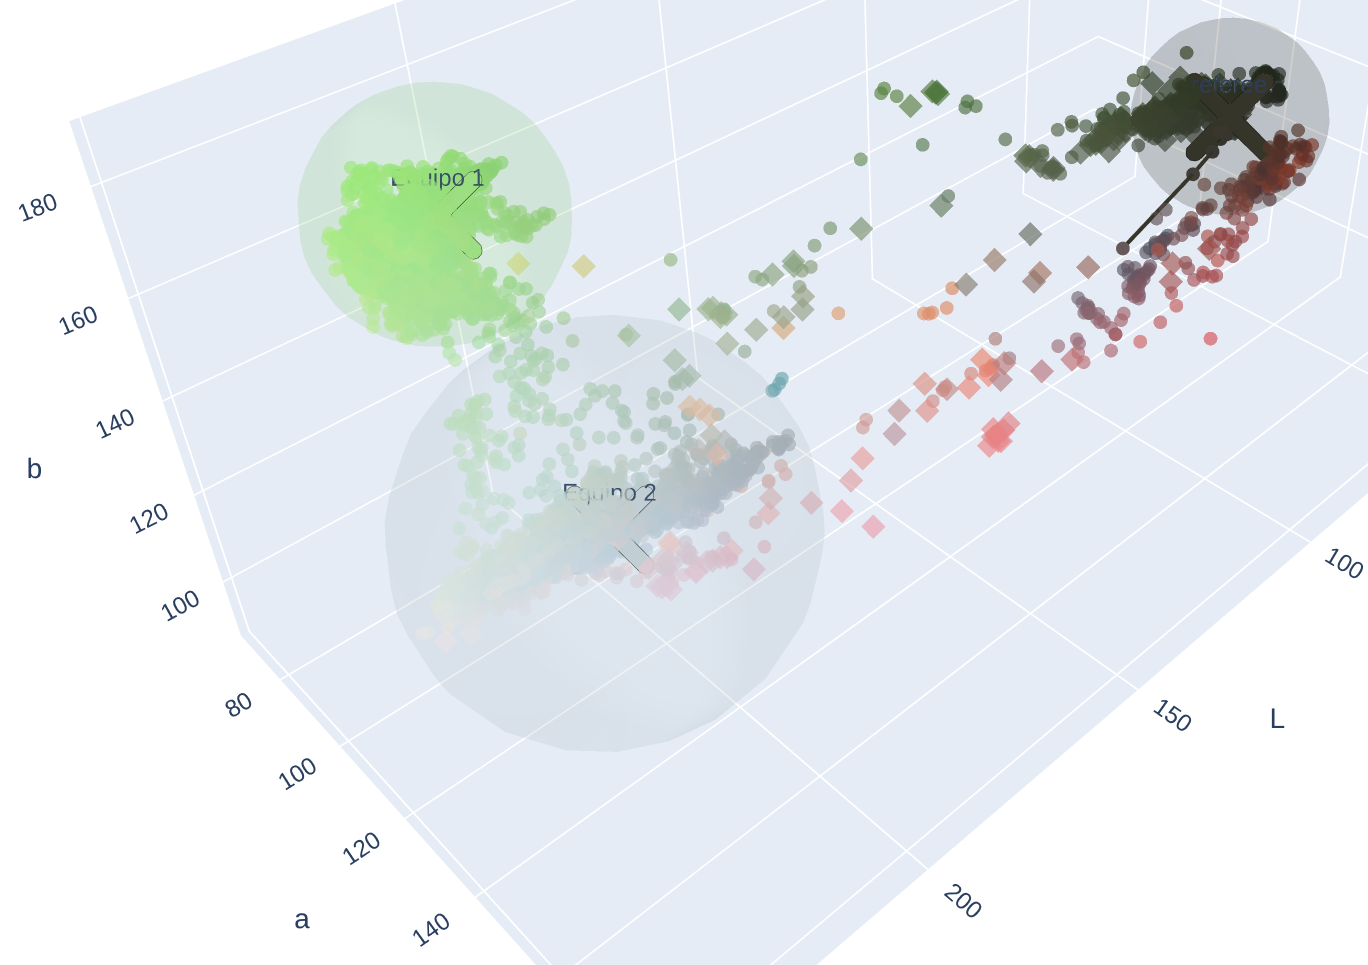
\includegraphics[width=0.7\textwidth]{Imagenes/Propias//lab_scatter_3d.png}
    \caption[Distribución de detecciones en el espacio LAB]{Distribución de detecciones en el espacio LAB, referencias de color y fronteras de pertenencia por equipo.}
    \label{fig:team-color-clusters-lab}
\end{figure}

\subsubsection{Reetiquetado de clase}

Una vez disponible el estado de color (centros de equipo, referencia de árbitro y umbrales de pertenencia), la inferencia por detección no se limita a asignar equipo: también puede reajustar la clase semántica final de la detección. En concreto, para cada candidato con color de camiseta estimado se calcula su distancia a los centros disponibles y, junto con restricciones posicionales en coordenadas de campo, se decide la etiqueta final entre \texttt{player}, \texttt{referee} y \texttt{goalkeeper}.

Si el color se asocia al patrón de árbitro, la detección solo se confirma como \texttt{referee} cuando también supera las compuertas posicionales definidas para ese rol (estar pegado a las líneas de banda o en una posición central del campo).

Cuando una detección queda fuera del patrón de equipos de campo pero su posición es compatible con portero, puede reetiquetarse como \texttt{goalkeeper}.

Para jugadores de campo, la pertenencia a equipo se valida además con umbrales robustos intra-cluster (derivados de cuartiles e IQR). Así, una detección no se acepta únicamente por vecino más cercano, sino también por consistencia estadística con el cluster de destino. 

En resumen, la salida de esta fase no es solo un color asignado a un equipo, sino una decisión conjunta \textit{clase + equipo} condicionada por evidencia cromática y geométrica, lo que mejora la robustez frente a confusiones entre jugador, árbitro y portero.

La \hyperref[fig:field-relabel-map]{Figura~\ref*{fig:field-relabel-map}} muestra el funcionamiento del re-etiquetado sobre coordenadas de campo. En naranja se representan los casos en los que una detección inicial de \texttt{player} se reclasifica como \texttt{referee}, y en azul los casos \texttt{player}$\rightarrow$\texttt{goalkeeper}. La distribución espacial de estos puntos coincide con lo que se observa en el vídeo de referencia: los re-etiquetados naranjas se concentran en la zona central, consistente con la trayectoria del árbitro principal, mientras que los re-etiquetados azules aparecen en el entorno del área izquierda, compatible con la posición típica de un portero. Además, los cambios se producen únicamente dentro de las regiones de validez definidas por las compuertas posicionales de cada clase.


\begin{figure}[H]
    \centering
    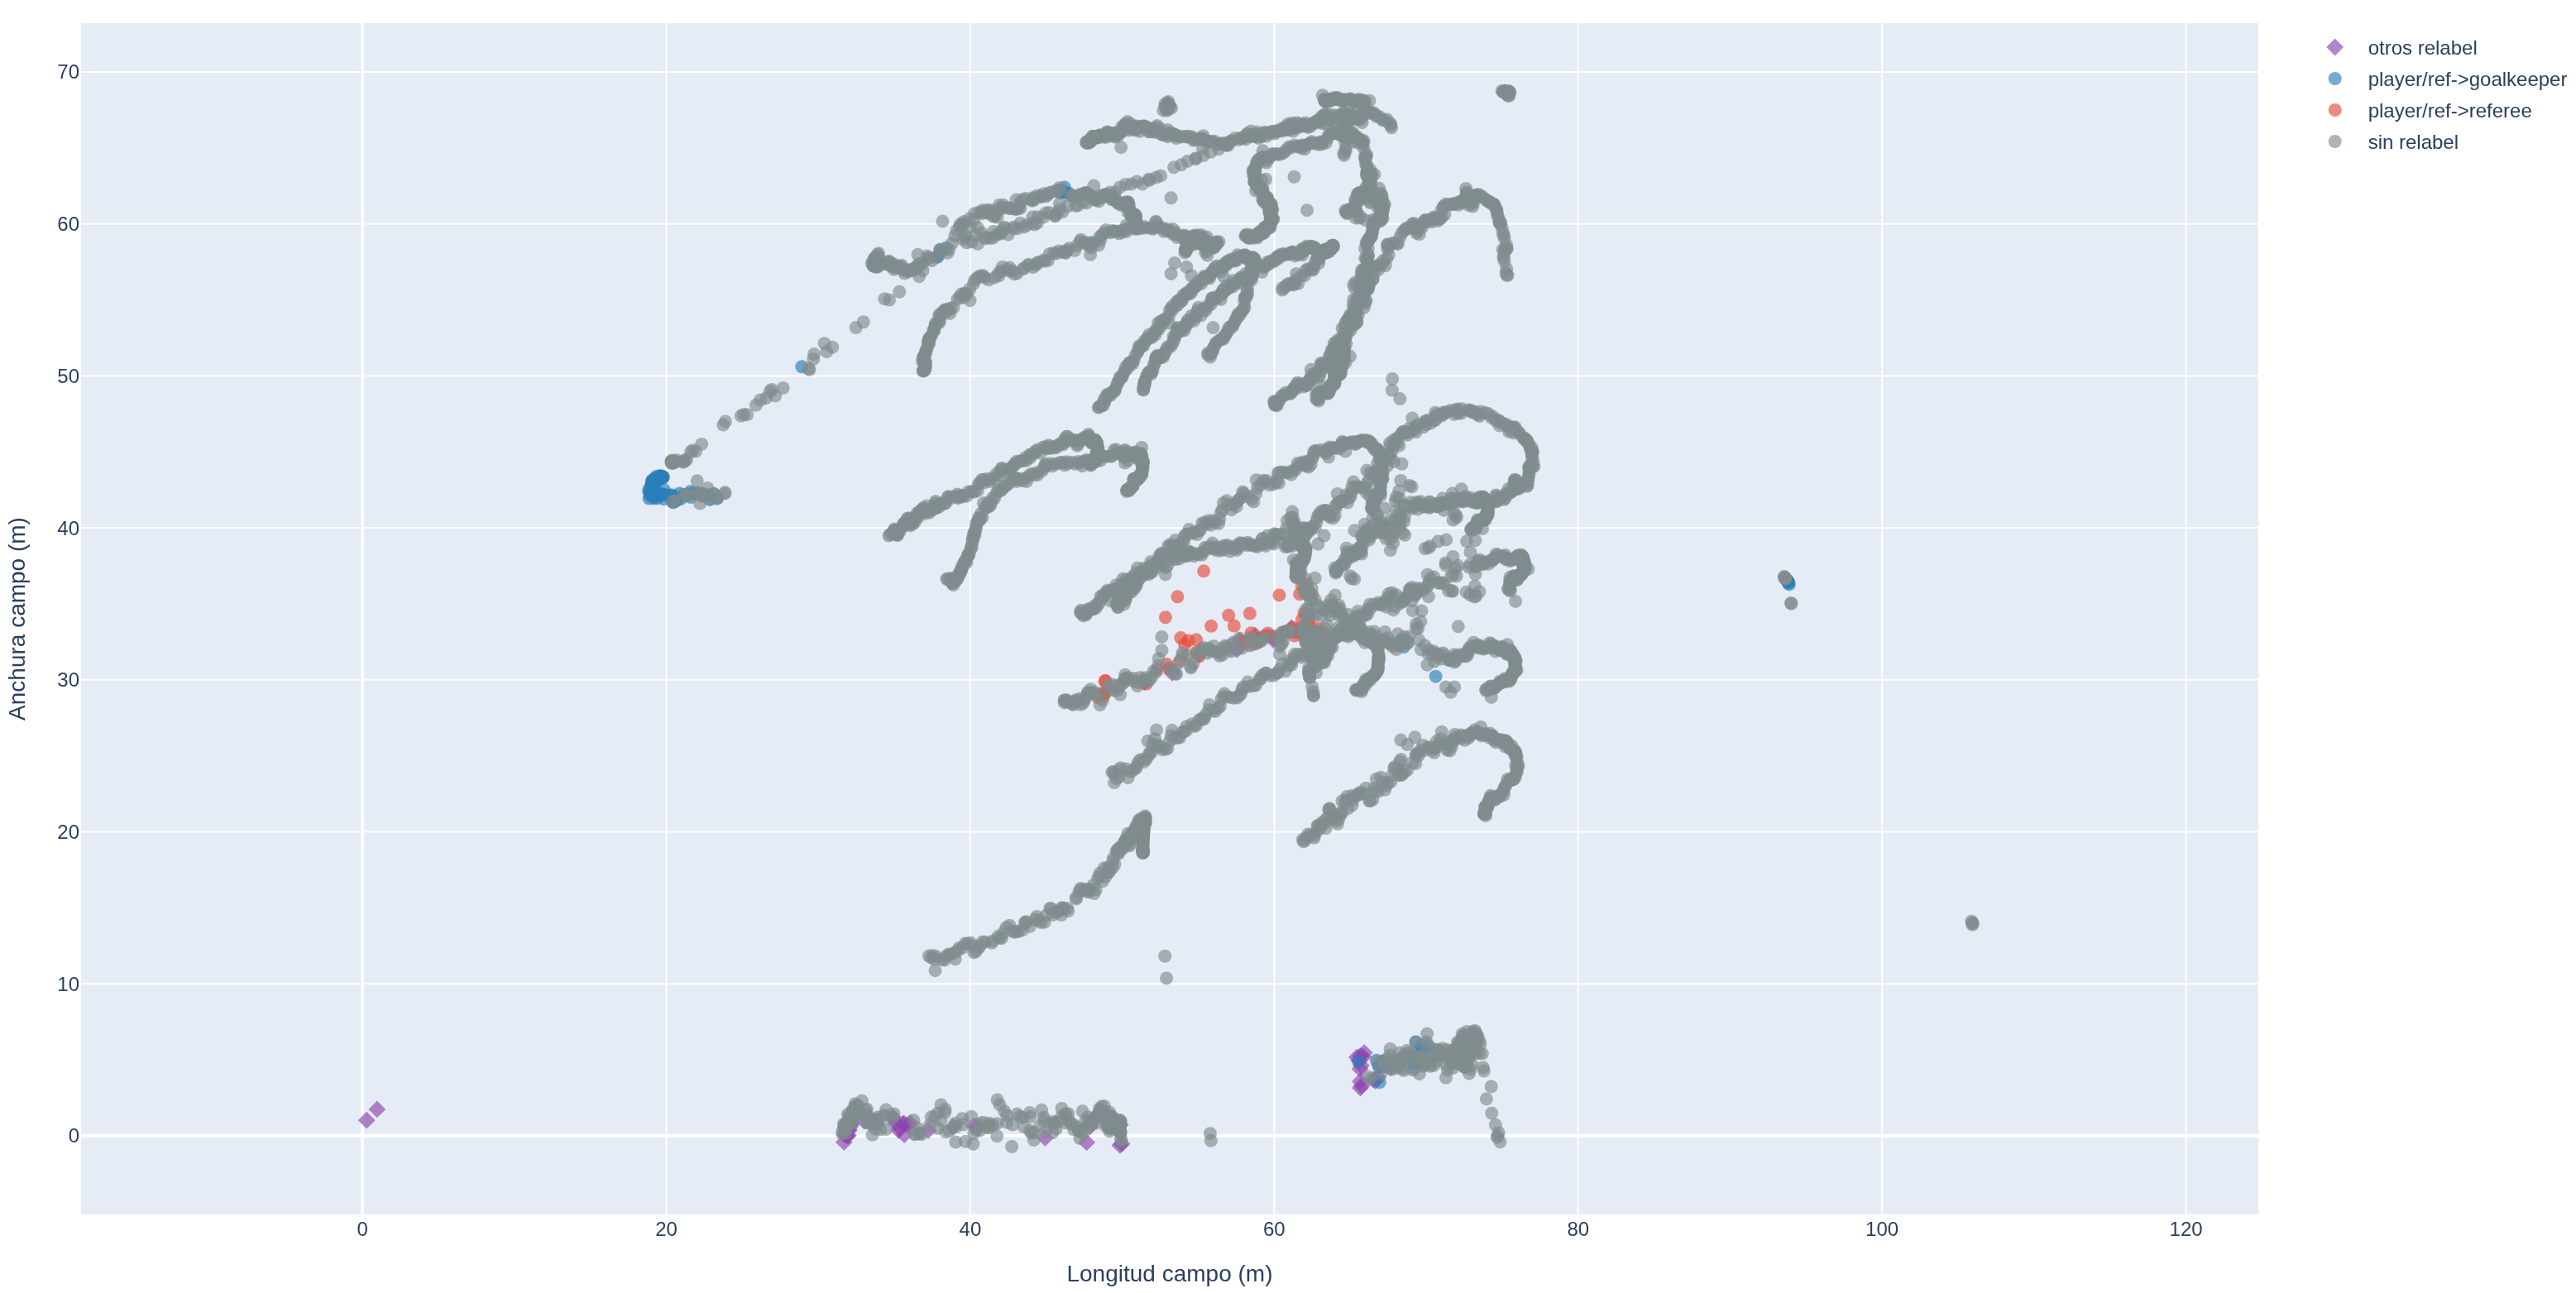
\includegraphics[width=0.95\textwidth]{Imagenes/Propias/field_relabel_map.png}
    \caption[Mapa de relabels en el campo]{Mapa de posiciones en campo con casos de relabel por categoría.}
    \label{fig:field-relabel-map}
\end{figure}


La configuración operativa del módulo se resume en la Tabla~\ref{tab:clasificacion_equipos}. 
\begin{table}[htbp]
    \centering
    \begin{tabular}{c|c}
        \textbf{Parámetro} & \textbf{Valor utilizado} \\
        \hline\hline
        Espacio de color & LAB \\
        Región analizada & 50\% superior del bounding box \\
        Clusters para camiseta & 2 \\
        Clusters para equipos de campo & 2 \\
        Muestras mínimas (\texttt{player}) & 60 acumuladas \\
        Muestras mínimas (\texttt{referee}) & 15 acumuladas \\
        Frecuencia de actualización de clusters & cada 5 frames \\
        Tamaño mínimo de cluster (\texttt{min\_size\_cluster}) & 15 \\
        Centro de equipo & mediana LAB del cluster \\
        Referencia de árbitro & \textit{trimmed mean} LAB (15\%) \\
        Distancia de asignación & euclídea en LAB \\
        \hline
    \end{tabular}
    \caption{Configuración principal del módulo de clasificación de equipos.}
    \label{tab:clasificacion_equipos}
\end{table}

Finalmente, cabe destacar que esta fase fue uno de los cuellos de botella iniciales del pipeline. En una primera versión, el clustering de cada camiseta se realizaba en CPU con \texttt{scikit-learn}, lo que incrementaba el tiempo de procesamiento por frame. Para reducir esta latencia se implementó una versión batched del KMeans con aceleración en GPU cuando está disponible (basada en \texttt{CuPy}), manteniendo \texttt{scikit-learn} como alternativa en CPU. En nuestras pruebas, esta optimización redujo el tiempo aproximado de identificación de camisetas y asignación de equipo de 1.5 s/frame a 0.05 s/frame, lo que supone una aceleración de aproximadamente $30\times$.


\section{Capa de asociacion temporal basada en ByteTrack}
\label{sec:bytetrack-layer}

El proceso de detección permite identificar que en un frame aparece un elemento de una determinada clase, pero cada frame se procesa de forma independiente. Para que el sistema pueda reconocer a un mismo jugador a lo largo del vídeo, no basta con detectar jugadores, porteros, árbitros y balón en cada imagen: es necesario asociar las detecciones de frames consecutivos y mantener una identidad temporal estable. Este proceso se conoce como \textit{tracking multiobjeto}.

En nuestro caso, el tracking es una fase crítica porque gran parte de la información posterior depende del identificador asignado a cada elemento. Si un jugador recibe un ID distinto cada vez que aparece, no es posible construir su trayectoria, asociarle una posición, vincularlo a una alineación o utilizarlo correctamente en la generación de eventos. Por ello, el objetivo no es únicamente dibujar bounding boxes sobre el vídeo, sino mantener una representación persistente del partido. Idealmente, la salida final debe estar limitada a los elementos reales del juego: 20 jugadores de campo, 2 porteros, 3 árbitros y 1 balón.

Esta fase ha sido una de las más complejas del proyecto. En fútbol aparecen muchos problemas propios del dominio: oclusiones entre jugadores, cruces continuos, jugadores del mismo equipo con apariencia muy parecida, cambios de escala por el zoom, movimientos de cámara, detecciones perdidas durante varios frames y elementos que salen temporalmente del plano. Además, intentar solucionar uno de estos problemas de forma aislada puede empeorar otro. Por ejemplo, permitir reasociaciones muy amplias ayuda a recuperar jugadores tras una oclusión, pero también aumenta el riesgo de intercambiar IDs entre jugadores cercanos. Por ello, el sistema se ha construido como una combinación de varias restricciones complementarias.

La fase de asociacion temporal se ha dividido en dos capas. La primera capa, tratada en esta seccion, es una adaptacion de ByteTrack orientada a producir asociaciones robustas entre detecciones consecutivas. La segunda capa, descrita en la \hyperref[sec:tracking-canonico]{Seccion~\ref*{sec:tracking-canonico}}, intenta coser esas asociaciones de ByteTrack para estabilizar las 26 identidades finales del partido.

En la \hyperref[sec:tracking-tecnologias]{Seccion~\ref*{sec:tracking-tecnologias}} se introdujo ByteTrack desde un punto de vista general. En este apartado se describe su integracion concreta como primera capa de tracking del pipeline visual y las modificaciones realizadas sobre el algoritmo clásico.

\subsection{Base de la fase}

Sobre la estructura original de ByteTrack se han añadido señales propias del proyecto: clase reajustada, equipo estimado y posicion proyectada sobre el campo.

La fase consume las detecciones enriquecidas de identificacion y produce una salida intermedia de detecciones asociadas con \textit{raw tracker id}. Esta salida no es todavia la identidad final del jugador, sino una asociacion temporal que alimentará la siguiente capa.

\subsection{Asociacion multi-etapa en cada frame}

Manteniendo la logica general explicada en la \hyperref[sec:tracking-tecnologias]{Figura~\ref*{sec:tracking-tecnologias}}, la implementacion actual ejecuta seis subfases de matching en vez de las 3 descritas en \hyperref[sec:tracking-tecnologias]{2.4}:
Manteniendo la logica general de ByteTrack descrita en la \hyperref[sec:tracking-tecnologias]{Sección~\ref*{sec:tracking-tecnologias}} (asociacion progresiva de tracks activos, perdidos y no confirmados), nuestra adaptación desdobla el matching en seis subfases, ampliando el esquema base presentado en 2.4.
\begin{itemize}
    \item \texttt{high\_iou}
    \item \texttt{low\_iou}
    \item \texttt{unconfirmed\_iou}
    \item \texttt{high\_bbox}
    \item \texttt{low\_bbox}
    \item \texttt{unconfirmed\_bbox}
\end{itemize}

Mientras que las primeras tres subfases usan el solape entre cajas como función de coste, las últimas 3 subfases, utilizan la distancias entre los centros de las \textit{bounding box}, y actuan como rescate cuando el solape no es suficiente, reduciendo fragmentaciones en escenas con zoom, paneos y discontinuidades de deteccion.

\subsection{Restricciones por clase y equipo}

Otra mejora introducida sobre ByteTrack consiste en utilizar la clase del objeto y el equipo asignado como restricciones de asociación. Si un ID canónico corresponde a un jugador, no debería poder reasociarse con una detección de balón o de árbitro. Del mismo modo, si un jugador pertenece a un equipo, no debería heredar la identidad de un jugador del equipo contrario.

Por lo tanto, en nuestra adaptación del ByteTrack, se usan la clase de la detección y su equipo asociado como restricciones de asociación duras. Si la clase del track y la clase de la deteccion candidata no coinciden, la asociacion se descarta automáticamente.

Del mismo modo, para \texttt{player}, cuando hay informacion de equipo tanto en el track como en la detección, se aplica también una restricción dura: si no coinciden, la asociacion se descarta.

Estas restricciones reducen los intercambios entre elementos de distinta clase y entre jugadores de equipos diferentes. Sin embargo, todavía puede haber intercambios entre jugadores del mismo equipo, especialmente cuando se cruzan o aparecen muy juntos en la imagen. Para reducir este problema fue necesario incorporar información geométrica del campo.

\subsection{Uso de homografia y restricción espacial en metros}

En nuestra versión de ByteTrack adaptada también se aplica un gate espacial en campo para las clases \texttt{player} y \texttt{goalkeeper}. Si la distancia proyectada entre el track y la detección candidata supera el límite configurado (8 metros), la asociación se descarta. En cambio, si está dentro del rango permitido, la pareja se mantiene como factible y el coste se decide por el criterio de matching de la subfase (IoU o distancia de centros en las fases de rescate).

Durante el desarrollo se evaluó usar la posición de las detecciones proyectada al campo como coste principal de la asociación. En la practica, esta opción degradaba el rendimiento ya que esta señal presentaba mucha vibracion frame a frame debido a pequeños cambios en la homografía entre frames.  Por este motivo había variaciones bruscas en las trayectorias estimadas de las identidades. Esto afectaba especialmente a la prediccion del estado con el filtro de Kalman y acababa propagando errores al proceso de matching. Por este motivo, en la version final la posicion en campo se utiliza como compuerta geometrica de factibilidad (gate duro) y no como termino principal de coste.

\subsection{Control de creacion de nuevos tracks}

Otro problema relevante es la creacion excesiva de nuevos tracks. Esto puede ocurrir cuando el detector produce bounding boxes duplicados o cuando ByteTrack pierde temporalmente una identidad. Para reducir este efecto, se añadieron reglas de supresión por solape de tracks nuevos:
\begin{itemize}
    \item contra tracks activos ya consolidados,
    \item contra tracks tentativos no confirmados,
    \item y entre candidatos nuevos del mismo frame.
\end{itemize}

Un candidato a track nuevo se descarta si solapa demasiado con un track activo, si solapa con un track tentativo no consolidado, o si solapa con otro candidato nuevo de mayor confianza. Ante cualquier solape entre dos candidatos nuevos, se conserva únicamente el de mayor confianza. Con esta regla se consigue reducir tracks duplicados sin alterar el seguimiento de tracks ya consolidados.

La configuración concreta de estos umbrales de solape se resume en la \hyperref[tab:supresion-nuevos-tracks-bytetrack]{Tabla~\ref*{tab:supresion-nuevos-tracks-bytetrack}}.

\begin{table}[htbp]
    \centering
    \scriptsize
    \begin{tabular}{c|c|p{7.5cm}}
        \textbf{Concepto} & \textbf{Valor} & \textbf{Funcion} \\
        \hline\hline
        Solape maximo con tracks activos & 0.2 & Evita crear un nuevo ID sobre un track ya consolidado. \\
        Solape maximo con tracks tentativos & 0.1 & Evita duplicados sobre tracks aun no consolidados. \\
        Solape entre candidatos nuevos & 0.0 & Conserva solo el candidato nuevo de mayor confianza si hay solape. \\
        \hline
    \end{tabular}
    \caption{Reglas de supresion en la creacion de nuevos tracks de ByteTrack.}
    \label{tab:supresion-nuevos-tracks-bytetrack}
\end{table}

\subsection{Resumen de la capa}

En resumen, esta fase no se limita a ejecutar ByteTrack sobre cajas de YOLO, sino que integra restricciones de clase, equipo, geometria en campo y control de creación de tracks para mejorar la asociacion temporal en video de futbol broadcast. La capa siguiente toma estas asociaciones y construye las identidades canonicas estables del partido.

\section{Capa de tracking canónico}
\label{sec:tracking-canonico}

La salida de la capa de asociación basada en ByteTrack (Seccion~\ref{sec:bytetrack-layer}) proporciona asociaciones robustas entre detecciones consecutivas de frames cercanos, pero esos IDs internos no garantizan por sí solos estabilidad global durante todo el partido. Cuando hay oclusiones largas, salidas de plano o cambios de escala bruscos, un mismo jugador puede reaparecer con otro \textit{tracker id}.

Por este motivo, el pipeline incorpora una segunda capa: la canonización. Su objetivo es transformar las asociaciones \textit{raw} en identidades finales estables, con límites por clase y reglas específicas para jugadores, porteros, árbitros y balón.

De esta forma, podría ocurrir que, por ejemplo, un jugador esté asociado al \textit{tracker id} 14 durante una parte del vídeo, se pierda durante varios frames y reaparezca con \textit{tracker id} 37. Si la capa canónica determina que ambos tracks corresponden al mismo jugador, entonces se conservará el mismo \textit{id canónico} para los dos tramos.

\subsection{Entrada de la capa y objetivo de canonización}

La capa canónica consume el paquete devuelto por la capa de ByteTrack y opera sobre detecciones ya asociadas, junto con metadatos de clase, equipo, posición en el campo y confianza. A partir de esa entrada, decide para cada detección si:
\begin{itemize}
    \item mantiene continuidad con un ID canonico existente,
    \item reengancha un ID canonico previo sobre un nuevo \textit{raw tracker id},
    \item crea una identidad canonica nueva dentro de los limites permitidos,
    \item o descarta la deteccion si no cumple los criterios de consistencia.
\end{itemize}

\subsection{Proceso de asignación canónica por frame}

En cada frame, la capa canónica aplica un flujo secuencial compacto. Primero intenta mantener continuidad directa entre \textit{raw tracker ids} ya conocidos y sus IDs canónicos previos, siempre que la compatibilidad de clase/equipo y las compuertas de continuidad sean válidas según la \hyperref[subsec:continuidad-canonica-reasignacion]{Subseccion~\ref*{subsec:continuidad-canonica-reasignacion}} y la \hyperref[subsec:reasignacion-sin-homografia]{Subseccion~\ref*{subsec:reasignacion-sin-homografia}}.

Despues, con los tracks de ByteTrack que no han sido resueltos en esa primera fase, se abre una fase de reasignación sobre IDs canónicos perdidos o libres, respetando de nuevo las reglas de continuidad en campo y en imagen definidas en la \hyperref[subsec:continuidad-canonica-reasignacion]{Subseccion~\ref*{subsec:continuidad-canonica-reasignacion}} y la \hyperref[subsec:reasignacion-sin-homografia]{Subseccion~\ref*{subsec:reasignacion-sin-homografia}}.
Si un track de ByteTrack sigue sin una asignación válida, la capa evalúa la creación de un nuevo slot canónico dentro de los límites y reservas definidos en la \hyperref[tab:limites-canonicos]{Tabla~\ref*{tab:limites-canonicos}} y explicados en la \hyperref[subsec:ids-canonicos-limites]{Subseccion~\ref*{subsec:ids-canonicos-limites}}.

Sobre ese flujo base se aplican reglas específicas por clase, detalladas en sus apartados correspondientes: porteros en la \hyperref[subsec:tratamiento-porteros]{Subseccion~\ref*{subsec:tratamiento-porteros}}, árbitros en la \hyperref[subsec:tratamiento-arbitros]{Subseccion~\ref*{subsec:tratamiento-arbitros}}, balón en la \hyperref[subsec:seguimiento-balon-canonico]{Subseccion~\ref*{subsec:seguimiento-balon-canonico}} y reabsorción conservadora en la \hyperref[subsec:reabsorcion-identidades]{Subseccion~\ref*{subsec:reabsorcion-identidades}}.

\subsection{IDs canónicos y límites por clase}
\label{subsec:ids-canonicos-limites}

A diferencia de ByteTrack, que puede crear tracks internos adicionales de forma flexible, la capa canónica impone una estructura final acotada.

En la configuración actual, los slots canónicos quedan reservados de forma explicita: el balón se fija en el ID 0, los porteros ocupan los IDs 1 y 2, los jugadores de campo se reparten en dos bloques por equipo (3--12 y 13--22), y, por último, los arbitros usan los IDs 23, 24 y 25. Además, los slots de árbitro no son intercambiables: 23 se asocia al arbitro central, 24 al asistente de la banda superior y 25 al asistente de la banda inferior. La \hyperref[tab:limites-canonicos]{Tabla~\ref*{tab:limites-canonicos}} resume esta asignación junto con los limites finales por clase.

\begin{table}[htbp]
    \centering
    \scriptsize
    \begin{tabular}{c|c|p{7.5cm}}
        \textbf{Parametro} & \textbf{Valor} & \textbf{Descripcion} \\
        \hline\hline
        \texttt{max\_tracks\_per\_class.player} & 20 & Jugadores de campo en slots canonicos de equipo (3--12 y 13--22). \\
        \texttt{max\_tracks\_per\_class.goalkeeper} & 2 & Porteros con IDs reservados (1 y 2). \\
        \texttt{max\_tracks\_per\_class.referee} & 3 & Arbitro central y asistentes con IDs reservados (23, 24, 25). \\
        \texttt{max\_tracks\_per\_class.ball} & 1 & Balon, almacenado siempre con ID 0. \\
        \hline
    \end{tabular}
    \caption{Limites de identidades canonicas por clase y asignacion de slots.}
    \label{tab:limites-canonicos}
\end{table}


\subsection{Continuidad canonica y reasignacion}
\label{subsec:continuidad-canonica-reasignacion}

Cuando hay posicion proyectada fiable en campo, la continuidad de \texttt{player}/\texttt{goalkeeper} se valida con un gate metrico dependiente de los frames perdidos. El gate parte de un valor base y crece de forma controlada hasta un maximo, evitando saltos fisicamente incompatibles y permitiendo recuperar identidades tras oclusiones cortas.

Siendo \(f\) el numero de frames desde la ultima observacion valida del ID canonico. El gate se calcula con base \(g_0=2.1\) m, decaimiento \(\delta=0.3\) m/frame, tope temporal \(f_{\max}=10\) y cap absoluto \(G_{\max}=8.0\) m:

\[
f'=\min(f,f_{\max}),
\qquad
G(f)=\min\!\left(
G_{\max},
\sum_{i=0}^{f'-1}\max(g_0-\delta i,0)
\right).
\]

Con los valores usados en el proyecto:

\[
G(1)=2.1,\;
G(2)=3.9,\;
G(3)=5.4,\;
G(4)=6.6,\;
G(5)=7.5,\;
G(6)=8.0,
\]

y a partir de ahi queda saturado en \(8.0\) m. Una candidata en campo se considera factible solo si su distancia al estado canonico cumple:

\[
d_{\text{campo}} \leq G(f).
\]

\subsection{Reasignación cuando no hay homografía fiable}
\label{subsec:reasignacion-sin-homografia}

Cuando no hay homografía válida, la capa canónica utiliza la posición en imagen como respaldo. En ese caso, no puede medir distancias en metros, por lo que utiliza el centro de la bounding box y el histórico de movimiento del track.

Si todavía no hay suficiente histórico, se permite únicamente una tolerancia mínima de 10 píxeles. Cuando el track ya tiene al menos 3 muestras de movimiento, se calcula el desplazamiento medio por frame, $\overline{d}$, y se estima cuánto podría haberse movido durante los frames perdidos:

\[
D_{esperado} =
\overline{d} \cdot \min(f,12) \cdot 0.75
\]

donde $f$ es el número de frames perdidos. El valor 12 actúa como límite máximo de extrapolación: aunque un jugador lleve perdido más frames, el radio de búsqueda no sigue creciendo indefinidamente. El factor 0.75 hace que esta estimación sea conservadora, evitando abrir demasiado el radio de búsqueda. La \hyperref[tab:movimiento-imagen]{Tabla~\ref*{tab:movimiento-imagen}} resume los valores de los hiperparámetros.

\begin{table}[htbp]
    \centering
    \scriptsize
    \begin{tabular}{c|c|p{7.5cm}}
        \textbf{Parametro} & \textbf{Valor} & \textbf{Funcion} \\
        \hline\hline
        \texttt{reassign\_min\_distance} & 10 px & Radio minimo cuando todavia no hay historico suficiente. \\
        \texttt{reassign\_motion\_growth\_cap\_frames} & 12 & Limita el numero de frames durante los que el radio de busqueda puede crecer. \\
        \texttt{reassign\_min\_samples} & 3 & Observaciones necesarias para estimar el desplazamiento medio. \\
        \texttt{reassign\_motion\_factor} & 0.75 & Reduce la distancia extrapolada para evitar reasociaciones demasiado amplias. \\
        \hline
    \end{tabular}
    \caption{Restricciones de movimiento usadas cuando no hay homografía fiable.}
    \label{tab:movimiento-imagen}
\end{table}

\subsection{Tratamiento específico de porteros}
\label{subsec:tratamiento-porteros}

Los porteros presentan un problema particular: en muchos planos tácticos o de inicio de jugada no aparecen en cámara. Si el sistema esperase únicamente a detectarlos, podrían recibir IDs tardíos o inestables. Para evitarlo, se crean dos identidades canónicas reservadas en los puntos de penalti del campo. Estas identidades se corresponden con los IDs 1 y 2.

Estas detecciones no proceden de YOLO, sino que son semillas sintéticas generadas a partir de la geometría del campo. Mientras no haya una detección real compatible, se almacenan con confianza 0 y sin equipo asignado. Cuando aparece una detección de clase \textit{goalkeeper} compatible, la capa canónica asigna ese track sintético a la detección compatible.

El radio de absorción desde el punto de penalti es de 20 metros. Aunque parece un valor alto, no significa que cualquier jugador pueda absorber el ID del portero. Primero, solo se consideran detecciones compatibles con la clase \texttt{goalkeeper}. Segundo, la semilla está situada en el punto de penalti, pero el portero real puede aparecer sobre la línea de gol, dentro del área pequeña, desplazado lateralmente o con error de homografía. Por eso se utiliza un radio amplio, protegido por la restricción de clase. La \hyperref[tab:seeds-porteros]{Tabla~\ref*{tab:seeds-porteros}} resume los hiperparametros de configuracion asociados a estas semillas canónicas de portero.

\begin{table}[htbp]
    \centering
    \scriptsize
    \begin{tabular}{c|c|p{7.5cm}}
        \textbf{Concepto} & \textbf{Valor} & \textbf{Función} \\
        \hline\hline
        \texttt{reserve\_penalty\_spot\_seed\_match\_distance\_m} & 20 m & Fija el radio maximo de absorcion entre una seed de portero y una deteccion real compatible. \\
        \hline
    \end{tabular}
    \caption{Configuración de identidades sintéticas reservadas para porteros.}
    \label{tab:seeds-porteros}
\end{table}

\subsection{Tratamiento específico de árbitros}
\label{subsec:tratamiento-arbitros}

También se reservan IDs específicos para los árbitros. En concreto, el ID 23 se asocia al árbitro central, el 24 al árbitro asistente de la parte superior de la imagen y el 25 a su homólogo de la parte inferior. Esto se hace para no tratarlos como tres árbitros intercambiables y, así, evitar intercambios entre ellos.

Las detecciones de clase árbitro se asocian a uno de los tracks canónicos de árbitro de banda si su posición proyectada está a menos de 3 metros de la línea lateral.

Para el ID 23 asociado al árbitro central, se añade una restricción horizontal calculada a partir de los jugadores y porteros visibles. En cada frame se recogen las coordenadas $(x, y)$ proyectadas al campo de todas las detecciones y se ordenan por su coordenada $x$. Si existen al menos 4 posiciones válidas, se define como rango permitido el intervalo entre la segunda posición más a la izquierda y la segunda posición más a la derecha. De esta forma, una detección muy extrema en el campo no puede absorber el ID del árbitro central. Si no hay suficientes jugadores proyectados, esta restricción horizontal no se aplica.

\subsection{Reabsorción de identidades perdidas}
\label{subsec:reabsorcion-identidades}

Debido a las reglas de continuidad anteriores, puede ocurrir que un jugador desaparezca durante un tramo largo y vuelva con un \textit{raw tracker id} nuevo. Si todos los IDs canónicos ya están creados, se han alcanzado los límites por clase definidos en la \hyperref[tab:limites-canonicos]{Tabla~\ref*{tab:limites-canonicos}} y ningún track canónico compatible está lo suficientemente cerca del raw track de ByteTrack como para absorberlo, entonces ese track se quedará perdido en el limbo sin materializarse como track canónico real y se perderá esa identidad. Para estos casos, la capa canónica incorpora una reabsorción forzada orientada a recuperar estos tracks perdidos de la forma más segura posible.

El mecanismo se activa solo para \texttt{player}. Primero se identifican IDs canónicos de jugador que llevan perdidos al menos 20 frames. En paralelo, se buscan tracks \textit{raw} huérfanos que no hayan sido asignados en el frame actual y que se hayan mantenido al menos 10 frames consecutivos con clase \texttt{player} y el mismo equipo.

Con esos candidatos, la capa construye emparejamientos posibles únicamente dentro del mismo equipo. Cuando hay varios candidatos compatibles, se prioriza la asociación con mayor consistencia espacial y temporal (menor distancia respecto al último estado canónico útil), de modo que el track huérfano más compatible se reenganche al ID canónico perdido.

De este modo, la reabsorción actúa como una vía de recuperación tardía, pero con condiciones estrictas de clase, equipo y consistencia espacial.

\subsection{Seguimiento del balón}
\label{subsec:seguimiento-balon-canonico}

El balón se gestiona de forma distinta a los jugadores. Es un objeto más pequeño, con menor confianza de detección y movimientos más bruscos. Por ello, además de las detecciones devueltas por ByteTrack, se conservan candidatas crudas de YOLO con una confianza mínima muy baja, y la capa canónica selecciona una única candidata por frame.

Si el balón ya había sido visto recientemente, se estima una posición esperada a partir de su movimiento inmediato anterior (desplazamiento entre las últimas observaciones válidas) y se proyecta esa tendencia sobre los frames perdidos. Con esa predicción se aplica un gate posicional dinámico: parte de un radio base de 90 píxeles y crece con los frames perdidos (35 píxeles por frame). En paralelo, también se comprueba la compatibilidad de tamaño para descartar cambios de escala no plausibles.

Cuando una candidata tiene confianza alta (\(\geq 0.6\)), las restricciones se relajan de forma controlada: tanto el radio posicional como el ratio de tamaño permitido se escalan por 1.4. Todas estas restricciones y configuraciones se reflejan en la \hyperref[tab:balon-tracking]{Tabla~\ref*{tab:balon-tracking}}.

Si ninguna candidata resulta coherente con la predicción temporal y las validaciones de tamaño, el sistema prefiere dejar el frame sin balón antes que aceptar una detección errónea. El balón se almacena siempre con ID canónico 0.

\begin{table}[htbp]
    \centering
    \scriptsize
    \begin{tabular}{c|c|p{7.5cm}}
        \textbf{Concepto} & \textbf{Valor} & \textbf{Función} \\
        \hline\hline
        \texttt{ball\_min\_conf} & 0.0035 & Permite considerar candidatas debiles antes del filtrado temporal. \\
        \texttt{ball\_expected\_position\_gate\_px} & 90 px & Define el radio base alrededor de la posicion esperada del balon. \\
        \texttt{ball\_expected\_position\_gate\_growth\_per\_frame} & 35 px & Amplia el gate posicional por cada frame perdido. \\
        \texttt{ball\_expected\_position\_confidence\_relax} & 1.4 & Relaja el gate posicional y el ratio de tamano cuando la candidata tiene alta confianza. \\
        \texttt{ball\_size\_ratio\_per\_frame} & 1.8 & Limita los cambios de escala plausibles entre observaciones consecutivas. \\
        \texttt{ball\_size\_min\_samples} & 5 & Numero minimo de observaciones para activar la comprobacion estadistica de tamano. \\
        \texttt{ball\_size\_std\_factor} & 3.0 & Factor multiplicativo usado en la banda estadistica de tamano aceptable. \\
        \texttt{ball\_size\_std\_floor} & 1.0 & Impone un suelo para que la banda estadistica de tamano no colapse. \\
        \texttt{ball\_max\_reassign\_lost\_frames} & 30 & Limita la ventana tras la que deja de intentarse continuidad con el ultimo estado valido del balon. \\
        \texttt{ball\_high\_conf\_override} & 0.6 & Define el umbral a partir del cual una candidata se trata como deteccion de alta confianza. \\
        \hline
    \end{tabular}
    \caption{Restricciones temporales utilizadas para seleccionar el balón.}
    \label{tab:balon-tracking}
\end{table}

La configuracion de esta capa se resume en la \hyperref[tab:hiperparametros-canonico]{Tabla~\ref*{tab:hiperparametros-canonico}}. Esta tabla final solo recoge los parametros del bloque de track \texttt{canonical} que no se han detallado ya en tablas especificas anteriores de esta misma seccion.

\begin{table}[htbp]
\centering
\scriptsize
\setlength{\tabcolsep}{3pt}
\renewcommand{\arraystretch}{1.12}
\begin{tabularx}{\textwidth}{
>{\raggedright\arraybackslash}p{2.6cm}
>{\raggedright\arraybackslash}p{3.4cm}
>{\raggedright\arraybackslash}p{1.5cm}
>{\raggedright\arraybackslash}X
}
\toprule
\textbf{Bloque} & \textbf{Parámetro} & \textbf{Valor} & \textbf{Uso en pipeline} \\
\midrule

Continuidad en campo &
\texttt{field\_gate\_m} &
\texttt{2.1} &
Controla la distancia máxima permitida para reasignar tracks usando posición proyectada al campo. \\

&
\texttt{field\_max\_lost} &
\texttt{10} &
Limita el número de frames perdidos durante los que se permite recuperar una identidad mediante continuidad en campo. \\

&
\texttt{field\_gate\_cap\_m} &
\texttt{8.0} &
Acota el radio máximo de búsqueda en coordenadas métricas. \\

&
\texttt{field\_decay} &
\texttt{0.3} &
Reduce progresivamente la tolerancia de reasignación a medida que el track lleva más tiempo perdido. \\

\midrule

Reglas de árbitro &
\texttt{ref\_sideline\_band\_m} &
\texttt{3.0} &
Restringe los slots de árbitro de banda y ayuda a evitar intercambios entre árbitros. \\

\midrule

Reabsorción forzada &
\texttt{forced\_abs\_min\_lost} &
\texttt{20} &
Permite recuperar de forma tardía tracks huérfanos de jugadores solo tras un número mínimo de frames perdidos. \\

&
\texttt{forced\_abs\_min\_consist} &
\texttt{10} &
Exige consistencia temporal antes de reabsorber un raw track en una identidad canónica. \\

\bottomrule
\end{tabularx}

\caption[Hiperparámetros de la capa de tracking canónico]{
Hiperparámetros principales de la capa de tracking canónico.}
\label{tab:hiperparametros-canonico}
\end{table}

El valor final de los parámetros se describe en la \hyperref[sec:evaluacion-heuristica-depuracion]{Seccion~\ref*{sec:evaluacion-heuristica-depuracion}}.

\subsection{Salida del tracking}

La salida final del tracking se almacena como una estructura organizada por clase y por frame. Para cada elemento se guarda su bounding box, confianza, equipo asignado, color de camiseta, tamaño de la bounding box, ID interno de ByteTrack, ID canónico y posición proyectada al campo.

Esta información resulta fundamental para las fases posteriores del proyecto, ya que permite construir trayectorias, analizar estabilidad temporal, generar métricas y transformar los datos al formato requerido por los módulos de análisis de eventos.

En resumen, el tracking implementado combina detección, equipo, clase, homografía, restricciones geométricas, control de movimiento, límites por clase, IDs canónicos y reglas particulares para porteros, árbitros y balón. Esta combinación es necesaria para reducir pérdidas de identidad e intercambios entre jugadores en un escenario especialmente complejo como el vídeo broadcast de fútbol.

\section{Evaluacion heuristica y depuracion del pipeline visual}
\label{sec:evaluacion-heuristica-depuracion}

\subsection{Ausencia de \textit{ground truth} anotado}

Durante el desarrollo no se dispuso de un conjunto de datos anotado frame a frame que pudiera usarse como \textit{ground truth} para evaluar de forma supervisada todo el pipeline de procesamiento visual. Por ese motivo, la validacion del sistema se apoyo en una estrategia heuristica, combinando inspeccion visual y metricas agregadas tras cada ejecucion.

En particular, la inspeccion cualitativa se realizo sobre un video de prueba de referencia\footnote{\url{https://github.com/hectorgarciaa/narrador-futbol/blob/main/data/partidoPrueba/partido.mp4}}, revisando la evolucion temporal de las identidades y la consistencia de los tracks en situaciones dificiles (oclusiones, cruces, perdidas temporales y reapariciones).

\subsection{Metricas heuristicas principales}

Tras ejecutar el tracking, el sistema calcula un resumen de metricas para jugadores y balon. Entre ellas se incluyen la cobertura media, que mide durante que proporcion del video aparece cada ID; el numero medio de fragmentos, que indica cuantas interrupciones tiene una trayectoria; la longitud media de los huecos sin deteccion; la velocidad media y maxima estimada a partir del movimiento de las \textit{bounding boxes}; la tasa de cambios de equipo asignado; la entropia del equipo, que refleja la inestabilidad en la asignacion; la variacion del color de camiseta; la variacion del tamano de la \textit{bounding box}; y la confianza media de las detecciones asociadas a cada track.

\subsection{Uso de metricas para ajuste de hiperparametros}

Estas metricas fueron especialmente utiles para guiar la depuracion de todos los modulos visuales y no solo del tracking canonico. Por ejemplo, velocidades maximas excesivamente altas solian indicar intercambios de identidad entre jugadores lejanos; una cobertura baja podia senalar perdidas frecuentes de deteccion o \textit{gates} demasiado estrictos; y un numero alto de fragmentos apuntaba a trayectorias poco continuas.

Del mismo modo, cambios frecuentes de equipo o una alta variacion del color de camiseta podian revelar errores de clasificacion o reasignacion. Por tanto, la evaluacion del pipeline visual se apoyo en dos fuentes complementarias: inspeccion visual del video generado y analisis cuantitativo de metricas. La primera permitia entender el tipo de error y su contexto, mientras que la segunda permitia comparar ejecuciones y verificar si una modificacion mejoraba realmente la estabilidad global del sistema.




\textbf{IMAGEN DE 4 ID BYTETRACK ID CANONICOS ID FINALES Y BIRD EYE SIN POSICIONES}
\chapter{Análisis Táctico}
\label{cap:analisisTactico}

En el \hyperref[cap:procesamientoVisual]{Capítulo~\ref*{cap:procesamientoVisual}} se describió cómo el vídeo broadcast se transforma en una representación estructurada del partido: detecciones, equipos, posiciones proyectadas sobre el campo y tracks estables. A partir de esa base, este capítulo aborda una capa de interpretación de mayor nivel, orientada ya no a responder solo dónde está cada elemento, sino qué está ocurriendo futbolísticamente en la jugada.

Para ello, el capítulo se organiza en tres bloques. En primer lugar, se presenta una inferencia heurística de la posesión del balón a partir de la salida del tracking canónico. Después se describe el módulo de inferencia de posiciones futbolísticas, cuyo objetivo es asociar a cada jugador una función táctica dentro de la alineación y, contando con el once del equipo, identificar el jugador con nombre y apellidos. Por último, se expone la clasificación de acciones, donde las trayectorias y relaciones espaciales entre jugadores se transforman en eventos semánticos como pases, controles, robos o tiros.

\section{Inferencia heurística de la posesión}
\label{sec:inferencia-posesion}

A partir de la salida del procesamiento visual, el sistema dispone en cada frame de jugadores, porteros, árbitros y balón detectados, asociados temporalmente y proyectados sobre el campo. Sobre esta representación se implementa un módulo heurístico para estimar qué jugador y qué equipo tienen la posesión del balón en cada instante.

El método intenta resolver el problema mediante reglas basadas en proximidad, contacto y continuidad temporal. Para cada frame se localiza el balón y se calcula la distancia entre el balón y el punto inferior de la \textit{bounding box} del resto de detecciones. Además, se comprueba si el balón cae dentro de una región ampliada de la caja del jugador, lo que se considera una señal fuerte de posible control.

La decisión no depende únicamente de la distancia instantánea. También se tienen en cuenta señales dinámicas del balón, como reducciones bruscas de velocidad o cambios de dirección, que pueden indicar un toque. Asimismo, se incorpora continuidad temporal: si un jugador ya tenía la posesión en frames anteriores, el sistema tiende a mantenerla mientras el balón permanezca cerca y no exista evidencia clara de recuperación por parte de un rival. Para aceptar un cambio de posesión se exige una señal más fuerte o una confirmación durante varios frames, reduciendo así oscilaciones provocadas por ruido, oclusiones o errores del tracking.

Cuando no se detecta el balón durante varios frames, o cuando no existe ningún contacto consistente, la posesión se libera para evitar arrastrar una asignación antigua sin evidencia visual. La salida de este módulo es, por tanto, una estimación por frame del jugador poseedor, el equipo poseedor y la razón heurística asociada a la decisión.

Durante el desarrollo del proyecto nos pareció de vital importancia el cálculo de esta heurística ya que considerábamos que iba a ser una señal muy útil de cara a la detección de acciones. Sin embargo, dado el método final escogido para la detección de eventos (PathCRF), y teniendo en cuenta que este método utiliza únicamente la trayectoria de los jugadores como señal de entrada para su modelo, finalmente esta señal del poseedor de la posesión no se consume en ninguna etapa posterior del pipeline.

Durante el desarrollo del proyecto, la estimación heurística de la posesión se consideró una señal potencialmente muy relevante para la detección posterior de acciones. La intuición inicial era que conocer qué jugador o equipo tenía el balón podía facilitar la identificación del jugador protagonista de eventos como pases, controles, tiros o recuperaciones.

Sin embargo, la elección final de PathCRF como método de detección de eventos modificó este planteamiento. Este modelo utiliza como entrada principal las trayectorias de los jugadores y no requiere consumir explícitamente una señal previa de posesión estimada por el pipeline. Por este motivo, aunque el módulo de inferencia heurística de la posesión se implementó y resulta útil como herramienta de análisis y visualización, su salida no se utiliza finalmente como entrada directa en las etapas posteriores del sistema.

\section{Inferencia de posiciones futbolísticas}
\label{sec:clasificacion-posicional}

Esta sección describe el proceso seguido para inferir la posición futbolística de cada jugador a partir de su comportamiento espacial en el campo. En primer lugar, se motiva la necesidad de esta inferencia como paso intermedio entre el tracking y la identificación nominal de los futbolistas en la \hyperref[subsec:motivacion-inferencia-posicional]{Subsección~\ref*{subsec:motivacion-inferencia-posicional}}. A continuación, se define la tarea de clasificación posicional en la \hyperref[subsec:definicion-tarea-inferencia-posicional]{Subsección~\ref*{subsec:definicion-tarea-inferencia-posicional}} y se explica cómo se construyó y etiquetó el conjunto de datos utilizado en las \hyperref[subsec:dataset-inferencia-posicional]{Subsecciones~\ref*{subsec:dataset-inferencia-posicional}} y \hyperref[subsec:etiquetado-inferencia-posicional]{\ref*{subsec:etiquetado-inferencia-posicional}}. Posteriormente, se detallan las variables de entrada, la normalización táctica aplicada y la arquitectura del modelo empleado en las \hyperref[subsec:variables-inferencia-posicional]{Subsecciones~\ref*{subsec:variables-inferencia-posicional}}, \hyperref[subsec:normalizacion-tactica-campo]{\ref*{subsec:normalizacion-tactica-campo}} y \hyperref[subsec:arquitectura-modelo-posicional]{\ref*{subsec:arquitectura-modelo-posicional}}. Finalmente, se presentan el proceso de entrenamiento, la búsqueda de hiperparámetros, los resultados obtenidos y la asignación táctica final de posiciones en las \hyperref[subsec:entrenamiento-modelo-posicional]{Subsecciones~\ref*{subsec:entrenamiento-modelo-posicional}}, \hyperref[subsec:grid-search-posicional]{\ref*{subsec:grid-search-posicional}}, \hyperref[subsec:resultados-clase-posicional]{\ref*{subsec:resultados-clase-posicional}} y \hyperref[subsec:asignacion-tactica-final-posiciones]{\ref*{subsec:asignacion-tactica-final-posiciones}}.

\subsection{Motivación}
\label{subsec:motivacion-inferencia-posicional}

Tras la fase de detección y tracking, el sistema dispone de trayectorias asociadas a identificadores internos. Estos identificadores permiten seguir a los jugadores a lo largo del vídeo, pero no representan directamente la identidad real del futbolista. Es decir, el sistema puede saber que el jugador con ID 7 aparece en una determinada zona del campo durante varios frames, pero no sabe si ese jugador es el lateral izquierdo, el mediocentro o el delantero de su equipo.

Una posibilidad para resolver esta asociación sería reconocer el dorsal de la camiseta. Sin embargo, en vídeos de retransmisión esta opción es poco robusta. Los dorsales suelen aparecer con baja resolución, parcialmente ocultos, deformados por el movimiento, tapados por otros jugadores o visibles únicamente durante muy pocos frames. Además, la cámara no siempre muestra la espalda del jugador, por lo que depender del dorsal haría que la identificación fuera intermitente y frágil.

Por este motivo, en este trabajo se plantea una estrategia alternativa: inferir la posición futbolística de cada jugador a partir de su ubicación en el campo y de su relación espacial con sus compañeros. La idea es que, si un track se comporta espacialmente como el lateral izquierdo de un equipo, posteriormente puede asociarse con el jugador que ocupa esa posición en la alineación introducida antes del partido.

Por tanto, la inferencia posicional actúa como un puente entre el tracking geométrico y la identificación nominal de los jugadores.

\subsection{Definición de la tarea}
\label{subsec:definicion-tarea-inferencia-posicional}

La inferencia de posiciones se formula como un problema de clasificación supervisada. Cada muestra representa a un jugador concreto en un frame concreto, y el objetivo del modelo es predecir su rol futbolístico.

La taxonomía inicial contemplaba las siguientes etiquetas, descritas en la \hyperref[tab:abreviaturas_posiciones]{\ref*{tab:abreviaturas_posiciones}}:

\[
\texttt{POR}, \texttt{CI}, \texttt{LI}, \texttt{DFC\_IZQ}, \texttt{DFC\_CENT}, \texttt{DFC\_DER}, \texttt{LD}, \texttt{CD}, \texttt{MC}, \texttt{MI}, \texttt{MD}, \texttt{EI}, \texttt{ED}, \texttt{DC}
\]

\begin{table}[H]
\centering
\scriptsize
\begin{tabular}{c|l c|l c|l}
\textbf{Abrev.} & \textbf{Significado} & 
\textbf{Abrev.} & \textbf{Significado} & 
\textbf{Abrev.} & \textbf{Significado} \\
\hline\hline
\texttt{POR} & Portero & \texttt{CI} & Carrilero izquierdo & \texttt{CD} & Carrilero derecho \\
\texttt{LI} & Lateral izquierdo & \texttt{LD} & Lateral derecho & \texttt{MC} & Mediocentro \\
\texttt{DFC\_IZQ} & Defensa central izquierdo & \texttt{DFC\_CENT} & Defensa central central & \texttt{DFC\_DER} & Defensa central derecho \\
\texttt{MI} & Medio izquierdo & \texttt{MD} & Medio derecho & \texttt{DC} & Delantero centro \\
\texttt{EI} & Extremo izquierdo & \texttt{ED} & Extremo derecho & & \\
\end{tabular}
\caption[Abreviaturas de las posiciones futbolísticas]{Significado de las abreviaturas utilizadas para las posiciones futbolísticas.}
\label{tab:abreviaturas_posiciones}
\end{table}

Durante los experimentos se observó que las clases \texttt{CI} y \texttt{CD} eran especialmente problemáticas. Son posiciones menos frecuentes, aparecen principalmente en sistemas con defensa de cinco y tenían pocas muestras etiquetadas. Además, su comportamiento espacial es muy similar al de \texttt{LI} y \texttt{LD}. Por ello, tras las primeras pruebas se fusionaron con los laterales:

\[
\texttt{CI} \rightarrow \texttt{LI}, \qquad \texttt{CD} \rightarrow \texttt{LD}
\]

Por tanto, el modelo final trabaja con 11 clases de jugadores de campo:

\[
\texttt{LI}, \texttt{DFC\_IZQ}, \texttt{DFC\_CENT}, \texttt{DFC\_DER}, \texttt{LD}, \texttt{MC}, \texttt{MI}, \texttt{MD}, \texttt{EI}, \texttt{ED}, \texttt{DC}
\]

La clase \texttt{POR} no se aprende mediante el modelo. En su lugar, se asigna de forma heurística cuando el sistema de detección/tracking identifica al objeto como portero, como se explicó en la \hyperref[subsec:tratamiento-porteros]{Subsección~\ref*{subsec:tratamiento-porteros}}.

Para realizar esta tarea se procede a la construcción de un conjunto de datos etiquetados. En las siguientes secciones se describe cómo se lleva a cabo esta construcción, detallando el proceso de etiquetado, las variables utilizadas, las normalizaciones necesarias y la distribución de clases obtenida.

\subsection{Construcción del conjunto de datos}
\label{subsec:dataset-inferencia-posicional}

La construcción del conjunto de datos para la inferencia posicional se basó en material procedente del ecosistema del concurso \textit{DFL Bundesliga Data Shootout}, organizado por la DFL (Deutsche Fußball Liga) y publicado en Kaggle. El objetivo original de ese concurso no era la localización espacial de jugadores, sino la detección temporal de eventos de juego a partir de secuencias de vídeo, proporcionando clips de partido junto con anotaciones en ficheros CSV con el tipo de acción y su instante de ocurrencia. Por tanto, el conjunto de partida no incluía \textit{bounding boxes}, identidades de tracking ni etiquetas de posición futbolística.

A partir de ese material original surgieron dos derivados relevantes para este trabajo. Por un lado, una parte de los fotogramas fue anotada manualmente con \textit{bounding boxes} y clases de objetos del juego, dando lugar al conjunto publicado en Roboflow que se utiliza en la Sección~\ref{sec:deteccion-elementos-juego} para la detección de jugadores, porteros, árbitros y balón. Por otro lado, existe una re-publicación en Kaggle de los clips crudos de aproximadamente 30 segundos (750 frames a 25 FPS), pero sin anotaciones espaciales adicionales. Esta segunda variante es la que resulta útil en esta etapa, en la que, utilizando únicamente la secuencia visual como entrada, se etiqueta el rol táctico de cada jugador en cada frame.

\begin{table}[H]
\centering
\scriptsize
\renewcommand{\arraystretch}{1.2}
\begin{tabularx}{\textwidth}{
>{\raggedright\arraybackslash}p{4.0cm}
>{\raggedright\arraybackslash}X
}
\toprule
\textbf{Propiedad} & \textbf{Valor} \\
\midrule
Nombre del dataset &
\textit{DFL Bundesliga 460 MP4 Videos in 30Sec. + CSV} \\

URL &
\href{https://www.kaggle.com/datasets/saberghaderi/-dfl-bundesliga-460-mp4-videos-in-30sec-csv}{Kaggle - DFL Bundesliga 460 MP4 Videos in 30Sec. + CSV} \\

Procedencia &
Re-publicación en Kaggle de clips asociados al ecosistema del concurso \textit{DFL Bundesliga Data Shootout}. \\

Contenido &
Clips de vídeo en formato MP4 y ficheros CSV asociados. \\

Número de clips &
460 clips. \\

Duración por clip &
Aproximadamente 30 segundos. \\

Frecuencia de imagen &
25 FPS. \\

Frames por clip &
Aproximadamente 750 frames por clip. \\

Anotaciones disponibles &
Etiquetas temporales de evento en CSV en el dataset original/re-publicado. \\

Anotaciones espaciales &
No dispone de \textit{bounding boxes}, identidades de tracking ni etiquetas de posición futbolística. \\

Uso en este trabajo &
Fuente de clips crudos para generar tracks y construir un nuevo conjunto anotado manualmente con posiciones futbolísticas por jugador y frame. \\

\bottomrule
\end{tabularx}
\caption[Metadatos del dataset fuente de clips]{Resumen de las características del dataset de clips utilizado como punto de partida para la construcción del conjunto de datos de inferencia posicional.}
\label{tab:dataset_fuente_inferencia_posicional}
\end{table}

El primer paso consistió en procesar cada clip con el pipeline de procesamiento visual descrito en el \hyperref[cap:procesamientoVisual]{Capítulo~\ref*{cap:procesamientoVisual}} para obtener los tracks. A partir de estos tracks se construyó el dataset de inferencia posicional. La idea es que, si en un determinado frame se asigna manualmente una posición futbolística a un track, esa etiqueta puede propagarse a las observaciones posteriores del mismo track sin tener que etiquetar manualmente cada bounding box de cada frame. Por tanto, el tracking actúa como mecanismo intermedio para convertir un etiquetado manual escaso en un conjunto de muestras supervisadas mucho mayor.

Sin embargo, no todos los clips son igual de útiles para esta tarea. La calidad del tracking influye directamente en la calidad de las etiquetas propagadas. Si un jugador cambia de ID, si se generan falsos positivos o si un track tiene baja cobertura temporal, el dataset puede incorporar ruido. Por ello se analizaron métricas de tracking antes de decidir los clips finales que se utilizarán.

La métrica principal utilizada fue la cobertura del track. Esta mide la proporción de frames del vídeo en los que un jugador se mantiene detectado con un identificador asociado. Se consideraron dos valores agregados:

\begin{itemize}
    \item \textbf{Mean coverage}: cobertura media de los tracks del clip.
    \item \textbf{Median coverage}: cobertura mediana, más robusta frente a tracks atípicos.
\end{itemize}

Finalmente se usaron los 8 clips con mejores métricas de cobertura. Sus métricas se recogen en la \hyperref[tab:position_dataset_clips]{Tabla~\ref*{tab:position_dataset_clips}}. El dataset resultante contiene 114170 observaciones base y 109519 muestras supervisadas.

\begin{table}[H]
\centering
\scriptsize
\begin{tabular}{c|c|c|c|c}
\textbf{Clip} & \textbf{Mean coverage} & \textbf{Median coverage} & \textbf{Tracks} & \textbf{Samples} \\
\hline\hline
1 & 0.9198 & 0.9613 & 21 & 14131 \\
\hline
2 & 0.8976 & 0.9480 & 21 & 13834 \\
\hline
3 & 0.8913 & 0.9559 & 21 & 13794 \\
\hline
4 & 0.8763 & 0.9646 & 22 & 13603 \\
\hline
5 & 0.8563 & 0.9560 & 22 & 13437 \\
\hline
6 & 0.8681 & 0.9387 & 22 & 13471 \\
\hline
7 & 0.8641 & 0.9300 & 22 & 13630 \\
\hline
8 & 0.8572 & 0.9133 & 22 & 13619 \\
\hline
\end{tabular}
\caption[Resumen cobertura de clips utilizados]{Resumen de cobertura y número de muestras de los clips utilizados para entrenar el modelo de posiciones.}
\label{tab:position_dataset_clips}
\end{table}

\subsection{Proceso de etiquetado}
\label{subsec:etiquetado-inferencia-posicional}

El etiquetado no se realizó frame a frame, sino de forma periódica sobre un conjunto reducido de frames clave. En cada clip se seleccionaron 5 frames, aproximadamente cada 6 segundos. Esta selección no fue completamente rígida: dentro de una ventana temporal cercana al instante objetivo se escogió el frame con mayor número de jugadores trackeados, siempre que hubiera al menos 18 jugadores visibles.

En cada uno de estos frames se visualizaba una imagen con los identificadores de tracking sobre los jugadores, como se muestra en la \hyperref[fig:frame_etiquetado_posiciones]{Figura~\ref*{fig:frame_etiquetado_posiciones}}. A continuación, se asignaba manualmente a cada identificador una de las posiciones futbolísticas definidas en la taxonomía mediante un menú de etiquetado, mostrado en la \hyperref[fig:menu_etiquetado_posiciones]{Figura~\ref*{fig:menu_etiquetado_posiciones}}. Este menú fue desarrollado expresamente para facilitar el etiquetado posicional desde un notebook de Python. Dicho notebook forma parte del repositorio del proyecto, mencionado previamente en la \hyperref[sec:planTrabajo]{Sección~\ref*{sec:planTrabajo}}.

Una vez etiquetado un frame clave, la etiqueta asignada a cada track se propagaba temporalmente a las observaciones posteriores del mismo jugador (mismo track id) hasta alcanzar el siguiente frame clave. Para ello se utilizaba el ID del track como clave, de modo que todas las bounding boxes asociadas a ese track heredaban la misma posición mientras la identidad temporal se mantuviera estable.

Esta estrategia permite generar un número elevado de muestras sin etiquetar manualmente todos los frames del vídeo. Al mismo tiempo, evita extender una etiqueta durante todo el vídeo, lo cual sería peligroso si se produjera un cambio de identidad en el tracker.

\begin{figure}[H]
\centering
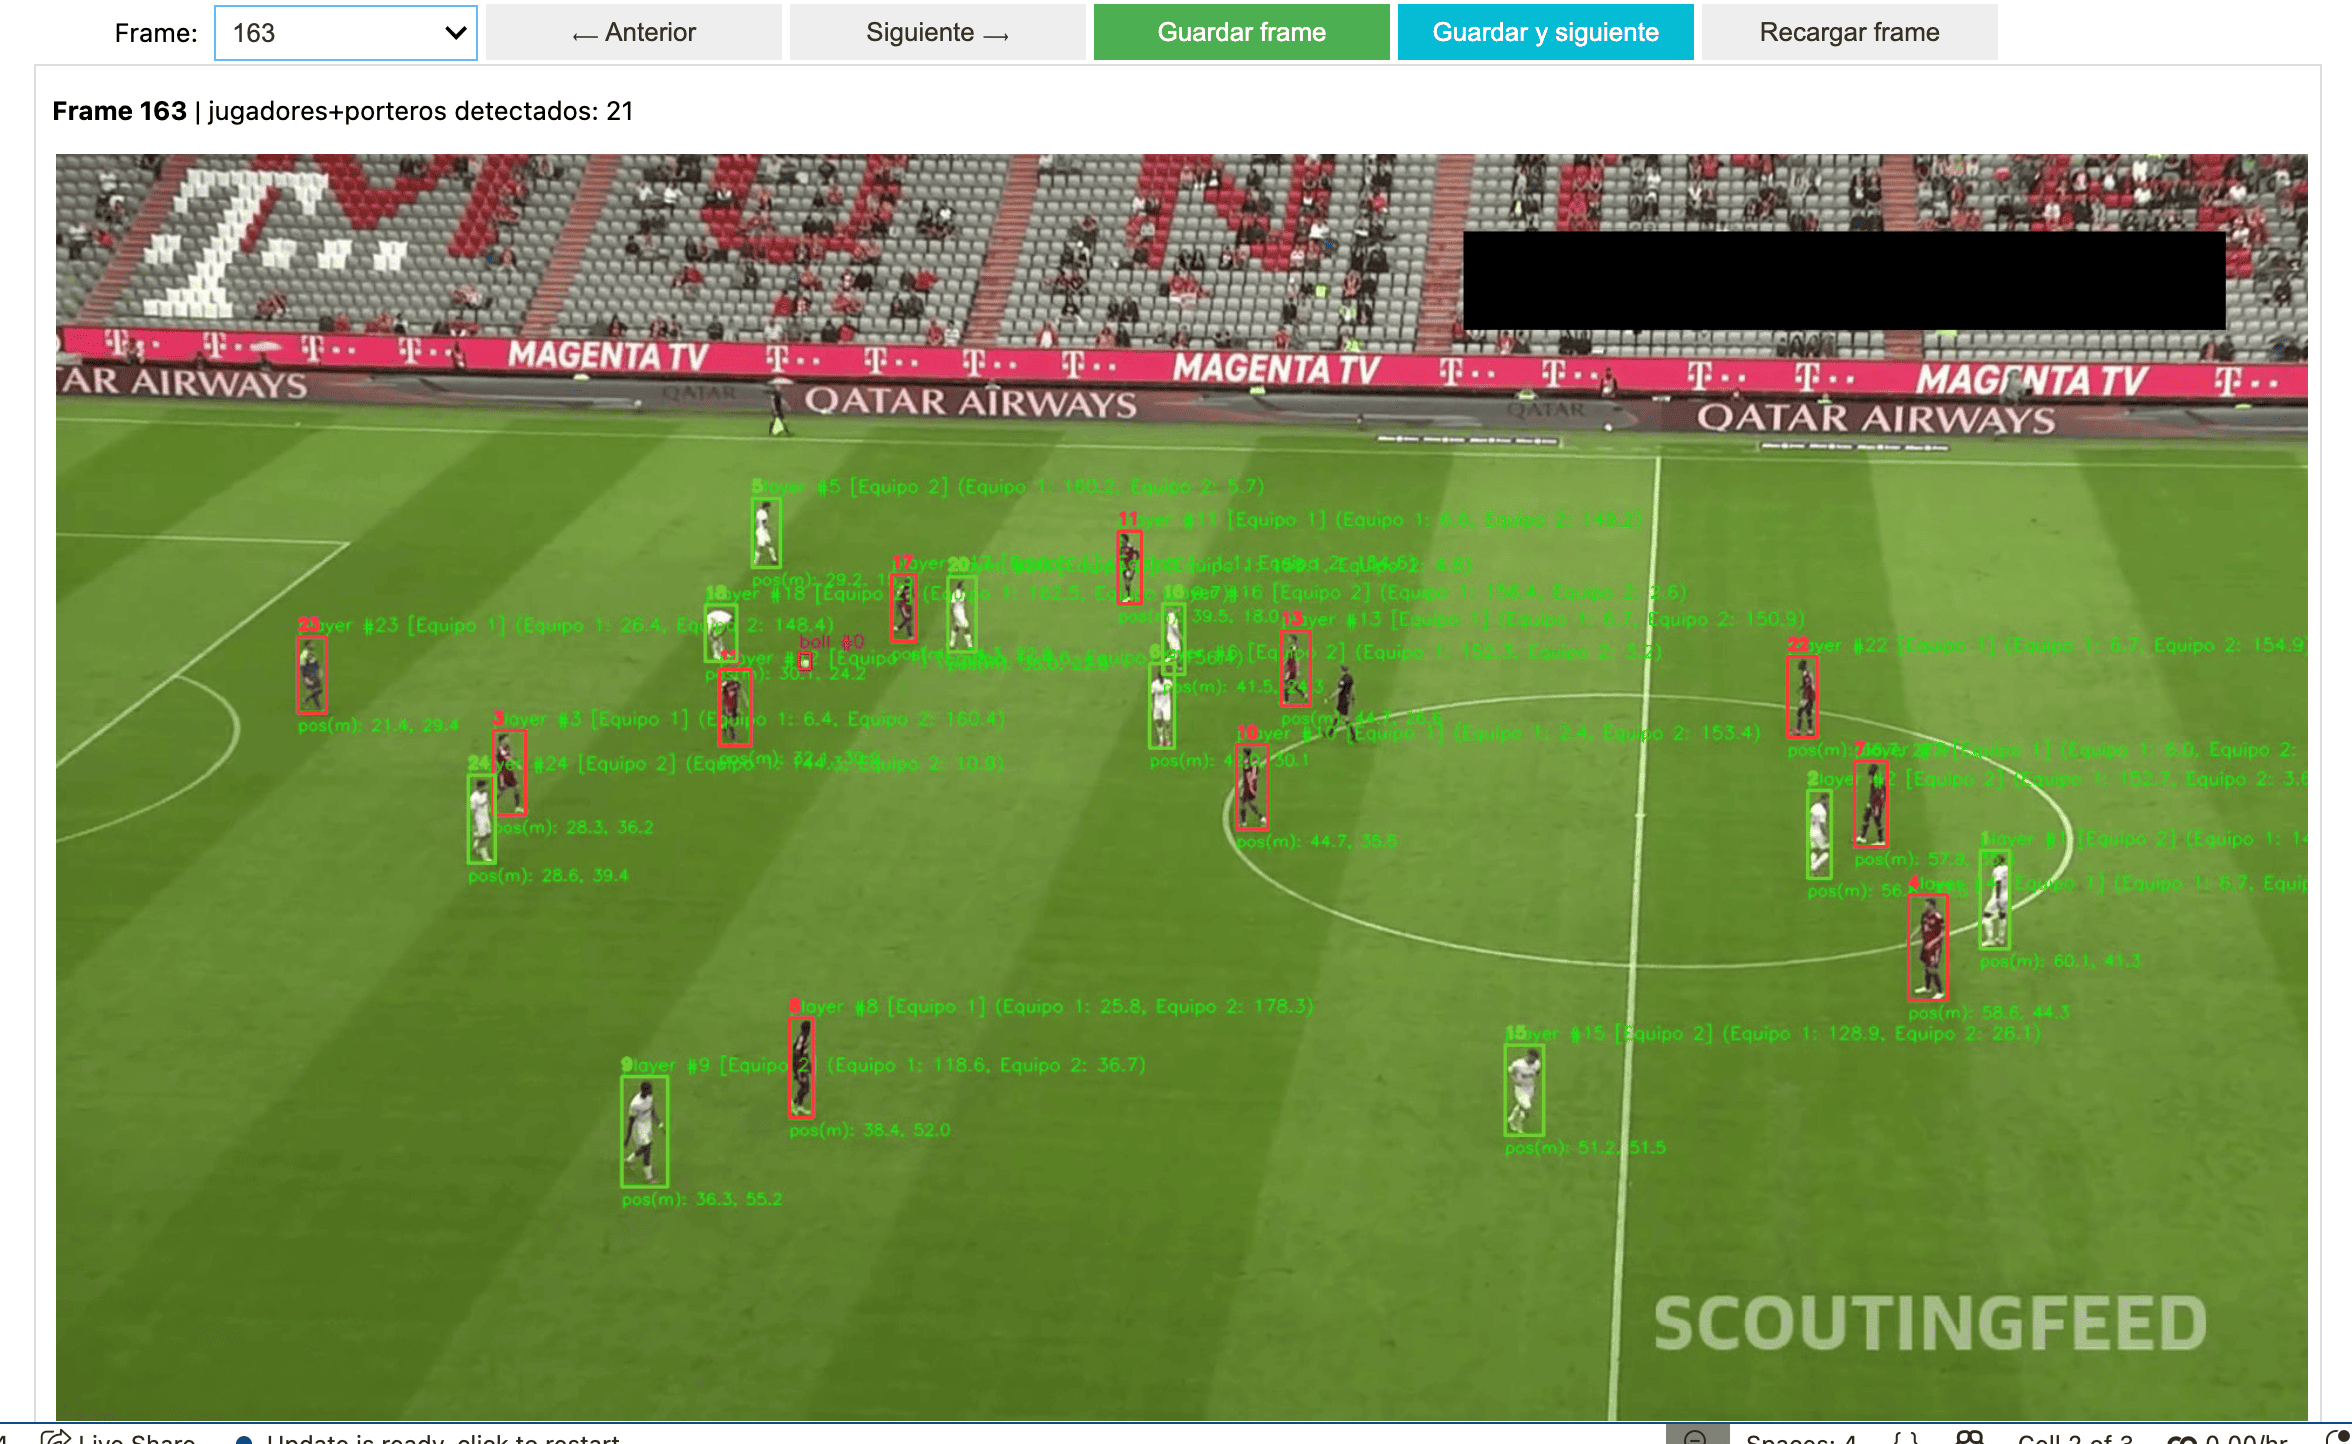
\includegraphics[width=0.49\linewidth]{Imagenes//Propias//Frame_a_etiquetar.png}
\caption[Frame de etiquetado posicional]{Frame con identificadores visibles sobre los jugadores para realizar el etiquetado posicional.}
\label{fig:frame_etiquetado_posiciones}
\end{figure}

\begin{figure}[H]
\centering
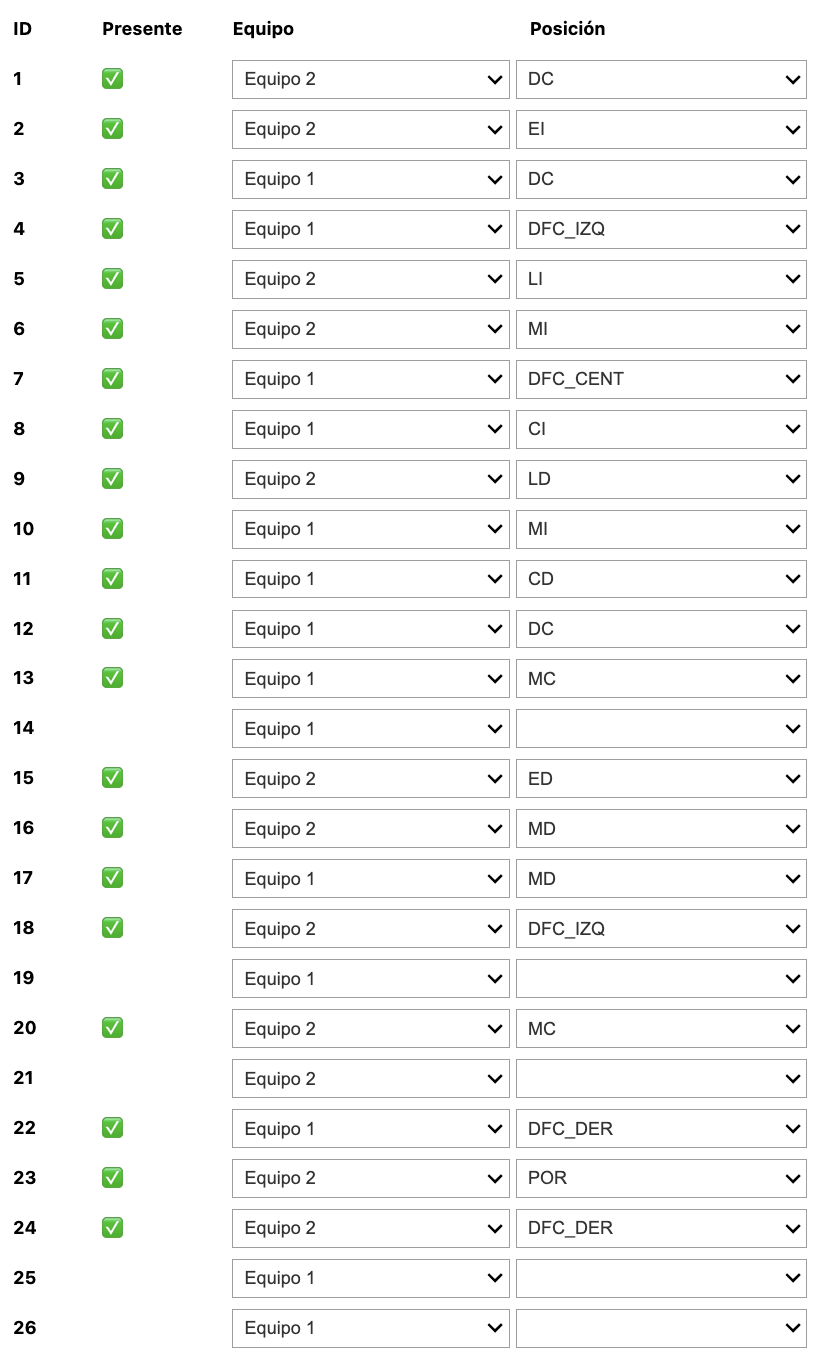
\includegraphics[width=0.49\linewidth]{Imagenes//Propias//Menu_para_etiquetar.png}
\caption[Menú de etiquetado posicional]{Menú de asignación de posición futbolística a cada identificador de tracking.}
\label{fig:menu_etiquetado_posiciones}
\end{figure}


\subsection{Normalización táctica del campo}
\label{subsec:normalizacion-tactica-campo}

Un aspecto clave es que los equipos atacan en direcciones opuestas. Sin una normalización previa, un lateral izquierdo de un equipo podría aparecer en coordenadas similares a un extremo derecho del rival. Para evitarlo, todas las muestras se transforman a una misma vista táctica antes de construir las variables de entrada del modelo.

La dirección de ataque no se introduce manualmente, sino que se infiere a partir de las observaciones del propio tracking. Cuando hay porteros detectados para ambos equipos, se toma como referencia la mediana de su coordenada normalizada \(x\): el equipo cuyo portero aparece más a la izquierda se considera asociado a la portería propia izquierda y, por tanto, se representa atacando hacia \(+x\), mientras que el otro equipo se representa atacando hacia \(-x\). Si no hay suficiente información fiable de porteros, se usa como respaldo la mediana de la coordenada \(x\) de todos los jugadores visibles del equipo.

Una vez estimada esta dirección, todas las muestras se reorientan para que ambos equipos queden expresados en el mismo sistema táctico. Si el equipo ataca hacia \(+x\), las coordenadas se mantienen. Si el equipo ataca hacia \(-x\), se aplica la transformación:

\[
x' = 1 - x, \qquad y' = 1 - y
\]

Con esta transformación, la portería propia de ambos equipos queda siempre en la misma referencia relativa, y las etiquetas izquierda/derecha conservan el mismo significado táctico independientemente del lado real del campo en el que esté jugando cada equipo.

Esta canonización es fundamental para que el modelo aprenda conceptos futbolísticos y no solo coordenadas absolutas dependientes del lado del campo. En caso contrario, dos jugadores con el mismo rol pero pertenecientes a equipos opuestos podrían ocupar regiones geométricamente parecidas en la imagen normalizada y, sin embargo, representar funciones tácticas distintas.


\subsection{Variables utilizadas}
\label{subsec:variables-inferencia-posicional}

Cada muestra del dataset representa a un jugador objetivo en un frame concreto. Para describirlo se utilizan dos bloques de información: variables propias del jugador y variables relativas a sus compañeros.

Las variables del jugador objetivo son:

\begin{itemize}
    \item \texttt{x}, \texttt{y}: coordenadas normalizadas del jugador en el campo.
    \item \texttt{dist\_left\_sideline}: distancia normalizada a la banda izquierda.
    \item \texttt{dist\_right\_sideline}: distancia normalizada a la banda derecha.
    \item \texttt{dist\_own\_goal}: distancia normalizada a la portería propia.
    \item \texttt{dist\_opponent\_goal}: distancia normalizada a la portería rival.
    \item \texttt{team\_centroid\_x}, \texttt{team\_centroid\_y}: centroide del equipo en ese frame.
    \item \texttt{dx\_centroid}, \texttt{dy\_centroid}: desplazamiento del jugador respecto al centroide del equipo.
    \item \texttt{rank\_x\_team}, \texttt{rank\_y\_team}: posición relativa del jugador dentro del equipo según los ejes del campo.
    \item \texttt{vx}, \texttt{vy}: velocidad normalizada estimada a partir del desplazamiento entre frames.
\end{itemize}

Las variables de compañeros describen el contexto espacial del jugador objetivo. Para cada compañero se incluyen:

\begin{itemize}
    \item \texttt{dx\_to\_obj}, \texttt{dy\_to\_obj}: desplazamiento relativo respecto al jugador objetivo.
    \item \texttt{dist\_to\_obj}: distancia euclídea al jugador objetivo.
    \item \texttt{x}, \texttt{y}: posición normalizada del compañero.
    \item Distancias del compañero a bandas y porterías.
    \item \texttt{vx}, \texttt{vy}: velocidad normalizada del compañero.
\end{itemize}

Se consideran como máximo 10 compañeros por muestra, ordenados por cercanía al jugador objetivo. Cuando hay menos de 10 compañeros disponibles, se rellena con ceros y se utiliza una máscara para indicar qué posiciones son reales y cuáles son padding. En el dataset final, la mediana de compañeros visibles por muestra es 9.

\subsection{Distribución de clases}

El dataset inicial presentaba un desbalanceo claro, como se muestra en la \hyperref[tab:position_class_distribution]{Tabla~\ref*{tab:position_class_distribution}}. Las clases \texttt{CI}, \texttt{CD} y \texttt{DFC\_CENT} eran las menos representadas. Tras fusionar los carrileros con los laterales, el reparto quedó más equilibrado, aunque \texttt{DFC\_CENT} siguió siendo la clase minoritaria.

\begin{table}[H]
\centering
\scriptsize
\begin{tabular}{c|c|c}
\textbf{Clase} & \textbf{Muestras antes del mapeo} & \textbf{Muestras finales} \\
\hline\hline
\texttt{CI} & 2816 & -- \\
\hline
\texttt{CD} & 2094 & -- \\
\hline
\texttt{LI} & 8013 & 10829 \\
\hline
\texttt{LD} & 7681 & 9775 \\
\hline
\texttt{DFC\_CENT} & 2897 & 2897 \\
\hline
\texttt{DFC\_IZQ} & 11896 & 11896 \\
\hline
\texttt{DFC\_DER} & 11345 & 11345 \\
\hline
\texttt{MC} & 10946 & 10946 \\
\hline
\texttt{MI} & 10562 & 10562 \\
\hline
\texttt{MD} & 11480 & 11480 \\
\hline
\texttt{EI} & 8095 & 8095 \\
\hline
\texttt{ED} & 8029 & 8029 \\
\hline
\texttt{DC} & 13665 & 13665 \\
\hline
\end{tabular}
\caption[Distribución de clases posicionales]{Distribución de clases antes y después de fusionar los carrileros \texttt{CI} y \texttt{CD} con los laterales \texttt{LI} y \texttt{LD}.}
\label{tab:position_class_distribution}
\end{table}


Una vez que se tiene el conjunto de datos etiquetado, se puede entrenar el modelo de inferencia de posiciones. Las secciones restantes de este capítulo se centran en explicar la arquitectura del modelo, su uso dentro del pipeline y en discutir los resultados obtenidos.


\subsection{Arquitectura del modelo}
\label{subsec:arquitectura-modelo-posicional}

El modelo utilizado es un Set Transformer. Como se mencionó en la \hyperref[sec:setTransformer]{Sección~\ref*{sec:setTransformer}}, esta arquitectura es adecuada porque el contexto de compañeros no es una secuencia ordenada, sino un conjunto. El orden en el que se introducen los compañeros no debería modificar la predicción. Si dos compañeros intercambian su posición en el tensor de entrada, la situación táctica sigue siendo la misma.

La entrada del modelo está formada por:

\begin{itemize}
    \item Un vector de 14 variables del jugador objetivo, descritas en la  \hyperref[subsec:variables-inferencia-posicional]{Sección~\ref*{subsec:variables-inferencia-posicional}}
    \item Un tensor de compañeros de tamaño $10 \times 11$.
    \item Una máscara binaria que indica qué compañeros existen realmente y cuáles son padding.
\end{itemize}

El modelo se divide en cuatro etapas principales, que se detallarán a continuación:

\begin{enumerate}
    \item Codificación del jugador objetivo.
    \item Codificación de cada compañero.
    \item Modelado del conjunto de compañeros mediante auto-atención.
    \item Agregación del conjunto y clasificación final.
\end{enumerate}

\subsubsection{Codificación del jugador objetivo}

El jugador objetivo se representa mediante sus 14 variables propias. Este vector se introduce en un MLP específica para el jugador objetivo, denotada como $MLP_{obj}$, que lo transforma en un embedding de dimensión fija. Este embedding resume la información individual del jugador: dónde está, a qué distancia se encuentra de bandas y porterías, cómo se sitúa respecto al centroide de su equipo y qué posición relativa ocupa dentro del bloque. Formalmente, si $x_{obj}$ es el vector de variables del jugador objetivo, se obtiene:

\[
h_{obj} = MLP_{obj}(x_{obj})
\]

donde $h_{obj}$ es el embedding individual del jugador. Esta MLP es distinta de la utilizada para codificar a los compañeros, ya que ambos tipos de entrada tienen diferente dimensionalidad y representan información distinta.

\subsubsection{Codificación de los compañeros}

Cada compañero se representa mediante 11 variables. Para codificarlos se utiliza una segunda MLP, denotada como $MLP_{comp}$, distinta de $MLP_{obj}$. Esta red se comparte entre todos los compañeros: es decir, la misma $MLP_{comp}$, con los mismos pesos aprendidos, se aplica de forma independiente a cada uno de los compañeros. De este modo, todos los compañeros se proyectan al mismo espacio latente. Formalmente, para cada compañero $i$ se calcula:

\[
h_i = MLP_{comp}(x_i)
\]

donde $x_i$ representa las variables del compañero $i$ y $h_i$ su embedding. El resultado es un conjunto de embeddings:

donde $x_i$ representa las variables del compañero $i$ y $h_i$ su embedding.

El resultado es un conjunto de embeddings:

\[
H = \{h_1, h_2, ..., h_n\}
\]

con $n \leq 10$. Si hay menos de 10 compañeros, los slots restantes se rellenan con ceros y se enmascaran.

\subsubsection{Bloques de auto-atención}

Sobre los embeddings de compañeros $H$ se aplican varios bloques de auto-atención multi-cabeza. Como se explicó en la \hyperref[sec:setTransformer]{Sección~\ref*{sec:setTransformer}}, este mecanismo permite que cada elemento del conjunto actualice su representación teniendo en cuenta al resto de elementos, sin imponer un orden secuencial sobre la entrada.

En esta implementación se utilizan bloques de auto-atención directa sobre el conjunto de compañeros, equivalentes al uso de bloques tipo SAB. No se emplean bloques ISAB, ya que el conjunto tiene un tamaño máximo de 10 compañeros y, por tanto, el coste cuadrático de la auto-atención completa no supone un problema relevante.

En cada bloque, los embeddings de los compañeros actúan simultáneamente como consultas, claves y valores:


\[
Q = HW_Q,\quad K = HW_K,\quad V = HW_V
\]

La atención se calcula como:

\[
Attention(Q,K,V)=softmax\left(\frac{QK^T}{\sqrt{d_k}}\right)V
\]

Esta operación permite aprender relaciones espaciales entre compañeros. Por ejemplo, para distinguir entre un lateral y un extremo no basta con mirar la posición del jugador objetivo; también puede ser relevante saber si tiene un compañero por delante, si forma parte de una línea defensiva, si está alineado con otros jugadores del centro del campo o si se encuentra aislado en la zona de ataque.

La atención multi-cabeza permite aprender varias relaciones espaciales en paralelo. Una cabeza puede especializarse en relaciones longitudinales, otra en relaciones laterales, otra en distancias al centroide y otra en estructuras de línea defensiva o línea ofensiva.

Tras la atención se aplica una conexión residual y una normalización:

\[
Z_1 = LayerNorm(H + Attention(H))
\]

Después se aplica una red feed-forward interna, seguida de otra normalización:

\[
Z_2 = LayerNorm(Z_1 + FFN(Z_1))
\]

La red feed-forward contiene una expansión de dimensión, activación \texttt{GELU} (Gaussian Error Linear Unit), dropout y una proyección de vuelta a la dimensión original. De esta forma, cada bloque combina relaciones entre compañeros mediante atención con transformaciones no lineales aplicadas a cada embedding.

\subsubsection{Pooling por atención}

Después de los bloques de auto-atención, el modelo dispone de un embedding contextualizado por cada compañero. Si hay \(n\) compañeros visibles, la salida de esta etapa puede escribirse como:

\[
Z \in \mathbb{R}^{n \times d}
\]

donde cada fila representa a un compañero y \(d\) es la dimensión del embedding. Sin embargo, para clasificar al jugador objetivo no se necesita una representación por compañero, sino un único vector que resuma el conjunto completo.

Para obtener este resumen se utiliza pooling por atención, basado en la idea de \textit{Pooling by Multihead Attention}, explicado también en \hyperref[sec:setTransformer]{Sección~\ref*{sec:setTransformer}}. Este mecanismo aplica la misma operación de atención descrita anteriormente, pero con una diferencia importante: las consultas no proceden de los compañeros, sino de un vector aprendible llamado \textit{seed} $S$. Este seed no representa a ningún jugador real, sino que actúa como una consulta global entrenable que aprende qué información debe extraerse del conjunto de compañeros para clasificar al jugador objetivo.

Formalmente, el pooling por atención puede escribirse como:

\[
PoolingAttention(S,Z) =
\operatorname{Attention}(SW_Q, ZW_K, ZW_V)
\]

Es decir, el seed genera la consulta \(Q\), mientras que los compañeros generan las claves \(K\) y los valores \(V\):
\[
Q = SW_Q,\quad K = ZW_K,\quad V = ZW_V
\]

donde \(S\) es el seed aprendible y \(Z\) son los embeddings de compañeros tras los bloques de auto-atención. A partir de estas matrices se calculan los pesos de atención:

\[
\alpha =
\operatorname{softmax}\left(\frac{QK^T}{\sqrt{d_k}}\right)
\]

y el resumen del conjunto se obtiene como una combinación ponderada de los valores:

\[
h_{set} = \alpha V
\]

De forma equivalente:

\[
h_{set} = PoolingAttention(S,Z)
\]


Como en este modelo se utiliza un único seed, el mecanismo produce una única salida. Por tanto, el pooling por atención reduce la dimensión asociada al número de compañeros, pasando de una representación \(n \times d\) a un único vector \(1 \times d\). Este vector resume el contexto táctico del jugador objetivo, dando más peso a los compañeros que el modelo considera más relevantes para la clasificación posicional.

\subsubsection{Clasificador final}

Finalmente, se concatena el embedding del jugador objetivo con el resumen del conjunto de compañeros:

\[
h = [h_{obj}; h_{set}]
\]

Este vector se introduce en un clasificador MLP que devuelve un logit por cada clase:

\[
logits = MLP_{cls}(h)
\]

Durante el entrenamiento se utiliza \texttt{CrossEntropyLoss}, que recibe directamente los logits. En inferencia, los logits se transforman en probabilidades mediante \texttt{softmax} y se selecciona la clase con mayor probabilidad.

\subsection{Entrenamiento}
\label{subsec:entrenamiento-modelo-posicional}

La separación del dataset se realizó por partido, no por muestras individuales. Esto es importante porque los frames consecutivos de un mismo clip son muy parecidos. Si se mezclaran frames del mismo clip entre entrenamiento y test, las métricas estarían sobreestimadas.

El split final contiene:

\begin{itemize}
    \item 82122 muestras de entrenamiento.
    \item 13603 muestras de validación.
    \item 13794 muestras de test.
\end{itemize}

Como se comenta en la sección anterior, el modelo produce, para cada muestra, un vector de logits \(z \in \mathbb{R}^{C}\), donde \(C\) es el número de clases posicionales. Estos logits se transforman en probabilidades mediante la función \textit{softmax}:

\[
p_c =
\frac{\exp(z_c)}
{\sum_{j=1}^{C} \exp(z_j)}
\]

donde \(p_c\) representa la probabilidad asignada a la clase \(c\).

Durante el entrenamiento se utilizó \texttt{CrossEntropyLoss}. Para una etiqueta real \(y\), la pérdida de entropía cruzada mide el desacuerdo entre la distribución objetivo y la distribución predicha por el modelo. En el caso básico, con etiquetas \textit{one-hot}, se expresa como:

\[
\mathcal{L} = - \log(p_y)
\]

donde \(p_y\) es la probabilidad predicha para la clase correcta.

Como el dataset presenta cierto desbalanceo entre clases, se utilizaron pesos de clase en la función de pérdida. Estos pesos se calcularon de forma inversamente proporcional a la frecuencia de cada clase en el conjunto de entrenamiento:

\[
w_c = \frac{N}{C \cdot n_c}
\]

donde \(N\) es el número total de muestras de entrenamiento, \(C\) es el número de clases y \(n_c\) es el número de muestras de la clase \(c\). De esta forma, los errores cometidos sobre clases poco representadas tienen mayor peso en la pérdida que los errores sobre clases frecuentes. La pérdida ponderada puede escribirse como:

\[
\mathcal{L} = - w_y \log(p_y)
\]

donde \(w_y\) es el peso asociado a la clase correcta.

Además, en el modelo final se aplicó \textit{label smoothing}. En lugar de entrenar con una etiqueta completamente concentrada en la clase correcta, se suaviza ligeramente la distribución objetivo. Para una muestra de clase real \(y\), la etiqueta suavizada se define como:

\[
\tilde{y}_c =
\begin{cases}
1 - \varepsilon + \frac{\varepsilon}{C}, & \text{si } c = y \\
\frac{\varepsilon}{C}, & \text{si } c \neq y
\end{cases}
\]

donde \(\varepsilon\) es el factor de suavizado. Con esta modificación, la pérdida pasa a calcularse sobre todas las clases:

\[
\mathcal{L} =
- \sum_{c=1}^{C} w_c \, \tilde{y}_c \log(p_c)
\]

El objetivo de esta técnica es evitar que el modelo se vuelva excesivamente confiado en sus predicciones. Esto resulta especialmente útil en esta tarea, ya que algunas posiciones futbolísticas son ambiguas desde el punto de vista espacial. Por ejemplo, un lateral, un interior y un extremo pueden ocupar zonas similares dependiendo de la fase de juego.

La métrica principal utilizada para seleccionar el mejor modelo fue el \textit{macro-F1}:
\[
MacroF1 =
\frac{1}{C}
\sum_{c=1}^{C} F1_c
\]

Esta métrica da el mismo peso a todas las clases, independientemente de su frecuencia. Por ello es más adecuada que la accuracy en un problema con clases desbalanceadas, ya que permite evaluar si el modelo funciona razonablemente bien también sobre las posiciones menos representadas.


\subsection{Grid search de hiperparámetros}
\label{subsec:grid-search-posicional}

Para optimizar el modelo se realizaron varios barridos de hiperparámetros. La \hyperref[tab:rejilla_grid_posiciones_base]{Tabla~\ref*{tab:rejilla_grid_posiciones_base}} resume la rejilla base utilizada en las Pruebas 1 y 3, mientras que la \hyperref[tab:rejilla_grid_posiciones_refine]{Tabla~\ref*{tab:rejilla_grid_posiciones_refine}} resume la rejilla de refinamiento usada en la Prueba 4. Cada prueba se evaluó con métricas agregadas y con su matriz de confusión en test, como se detalla a continuación.

\begin{table}[H]
\centering
\scriptsize
\resizebox{\textwidth}{!}{%
\begin{tabular}{c|c}
\textbf{Hiperparámetro} & \textbf{Valores explorados} \\
\hline\hline
Perfiles de anchura &
\((64,128,128,128),\ (128,256,192,256),\ (128,256,256,256),\ (256,384,256,384)\) \\
\hline
\texttt{objective\_num\_layers} & \(\{1,2\}\) \\
\hline
\texttt{ff\_expansion} & \(\{2,4\}\) \\
\hline
\texttt{num\_set\_blocks} & \(\{3,4,5\}\) \\
\hline
\texttt{learning\_rate} & \(\{10^{-3},\ 5\cdot10^{-4}\}\) \\
\hline
Regularización \((\texttt{dropout},\ \texttt{weight\_decay})\) &
\((0{.}10,\ 10^{-4});\ (0{.}15,\ 10^{-4});\ (0{.}20,\ 5\cdot10^{-4});\ (0{.}25,\ 5\cdot10^{-4});\ (0{.}30,\ 10^{-3})\) \\
\hline
Fijos & \(\texttt{batch\_size}=512,\ \texttt{num\_heads}=4,\ \texttt{epochs}=40\) \\
\hline
Núm. total de runs & \(480\) \\
\hline
\end{tabular}%
}
\caption[Rejilla base de las búsquedas de hiperparámetros]{Rejilla base utilizada en los barridos principales (Pruebas 1 y 3). Cada perfil de anchura se expresa como \((\texttt{teammate\_embed\_dim},\texttt{objective\_hidden\_dim},\texttt{set\_hidden\_dim},\texttt{fusion\_hidden\_dim})\), que corresponden respectivamente a la dimensión del embedding de compañeros, la dimensión oculta del codificador del jugador objetivo, la dimensión interna de los bloques de atención sobre el set y la dimensión de la capa de fusión previa al clasificador.}
\label{tab:rejilla_grid_posiciones_base}
\end{table}

\begin{table}[H]
\centering
\scriptsize
\resizebox{\textwidth}{!}{%
\begin{tabular}{c|c}
\textbf{Hiperparámetro} & \textbf{Valores explorados} \\
\hline\hline
Familias base & top-\(3\) de la Prueba 3 \\
\hline
\texttt{learning\_rate} & \(\{3\cdot10^{-4},\ 2\cdot10^{-4},\ 10^{-4}\}\) \\
\hline
\texttt{label\_smoothing} & \(\{0{.}05,\ 0{.}10\}\) \\
\hline
\texttt{weight\_decay} & \(\{7{.}5\cdot10^{-4},\ 1{.}5\cdot10^{-3},\ 2\cdot10^{-3}\}\) \\
\hline
\texttt{dropout} & \(\{0{.}18,\ 0{.}22,\ 0{.}27,\ 0{.}33,\ 0{.}35\}\) \\
\hline
Fijos & \(\texttt{batch\_size}=512,\ \texttt{num\_heads}=4,\ \texttt{epochs}=40\) \\
\hline
Núm. total de runs & \(108\) \\
\hline
\end{tabular}%
}
\caption[Rejilla de refinamiento de hiperparámetros]{Rejilla de refinamiento usada en la Prueba 4}
\label{tab:rejilla_grid_posiciones_refine}
\end{table}

\subsubsection{Prueba 1: grid search con 13 clases}
La primera búsqueda mantuvo la taxonomía inicial, con \texttt{CI} y \texttt{CD} como clases independientes. Se ejecutaron 480 combinaciones variando anchura de los embeddings y capas ocultas del modelo, profundidad del codificador del jugador objetivo, el número de bloques de atención, el factor de expansión de la capa de feed-forward y la regularización y optimización (\textit{dropout}, \textit{learning\_rate}, \textit{weight\_decay}). La mejor configuración alcanzó un \textit{macro-F1} de 0.3096 en validación y 0.4022 en test, tal y como muestra la \hyperref[tab:grid_13_metrics]{Tabla~\ref*{tab:grid_13_metrics}}

\begin{table}[H]
\centering
\scriptsize
\begin{tabular}{c|c|c|c}
\textbf{Conjunto} & \textbf{Accuracy} & \textbf{Macro-F1} & \textbf{Weighted-F1} \\
\hline\hline
Validación & 0.3779 & 0.3096 & 0.3684 \\
\hline
Test & 0.4223 & 0.4022 & 0.4158 \\
\hline
\end{tabular}
\caption{Métricas de la mejor configuración del grid search con 13 clases.}
\label{tab:grid_13_metrics}
\end{table}

En resumen, los mejores resultados de validación tendieron a concentrarse en configuraciones con regularización moderada-baja (\texttt{dropout}=0.10, \texttt{weight\_decay}=1e-4) y \texttt{learning\_rate}=5e-4. Por otro lado, la variación de anchura y profundidad del modelo no mostró un patrón dominante claro en esta prueba, lo que sugiere que, con 13 clases, el rendimiento estuvo más condicionado por la regularización que por incrementos de capacidad.

La matriz de confusión de la \hyperref[fig:confusion_grid_13]{Figura~\ref*{fig:confusion_grid_13}} muestra que \texttt{CI} y \texttt{CD} eran clases inestables. En muchos casos se confundían con laterales, extremos o interiores. Esta observación motivó la fusión de carrileros con laterales.


\begin{figure}[H]
\centering
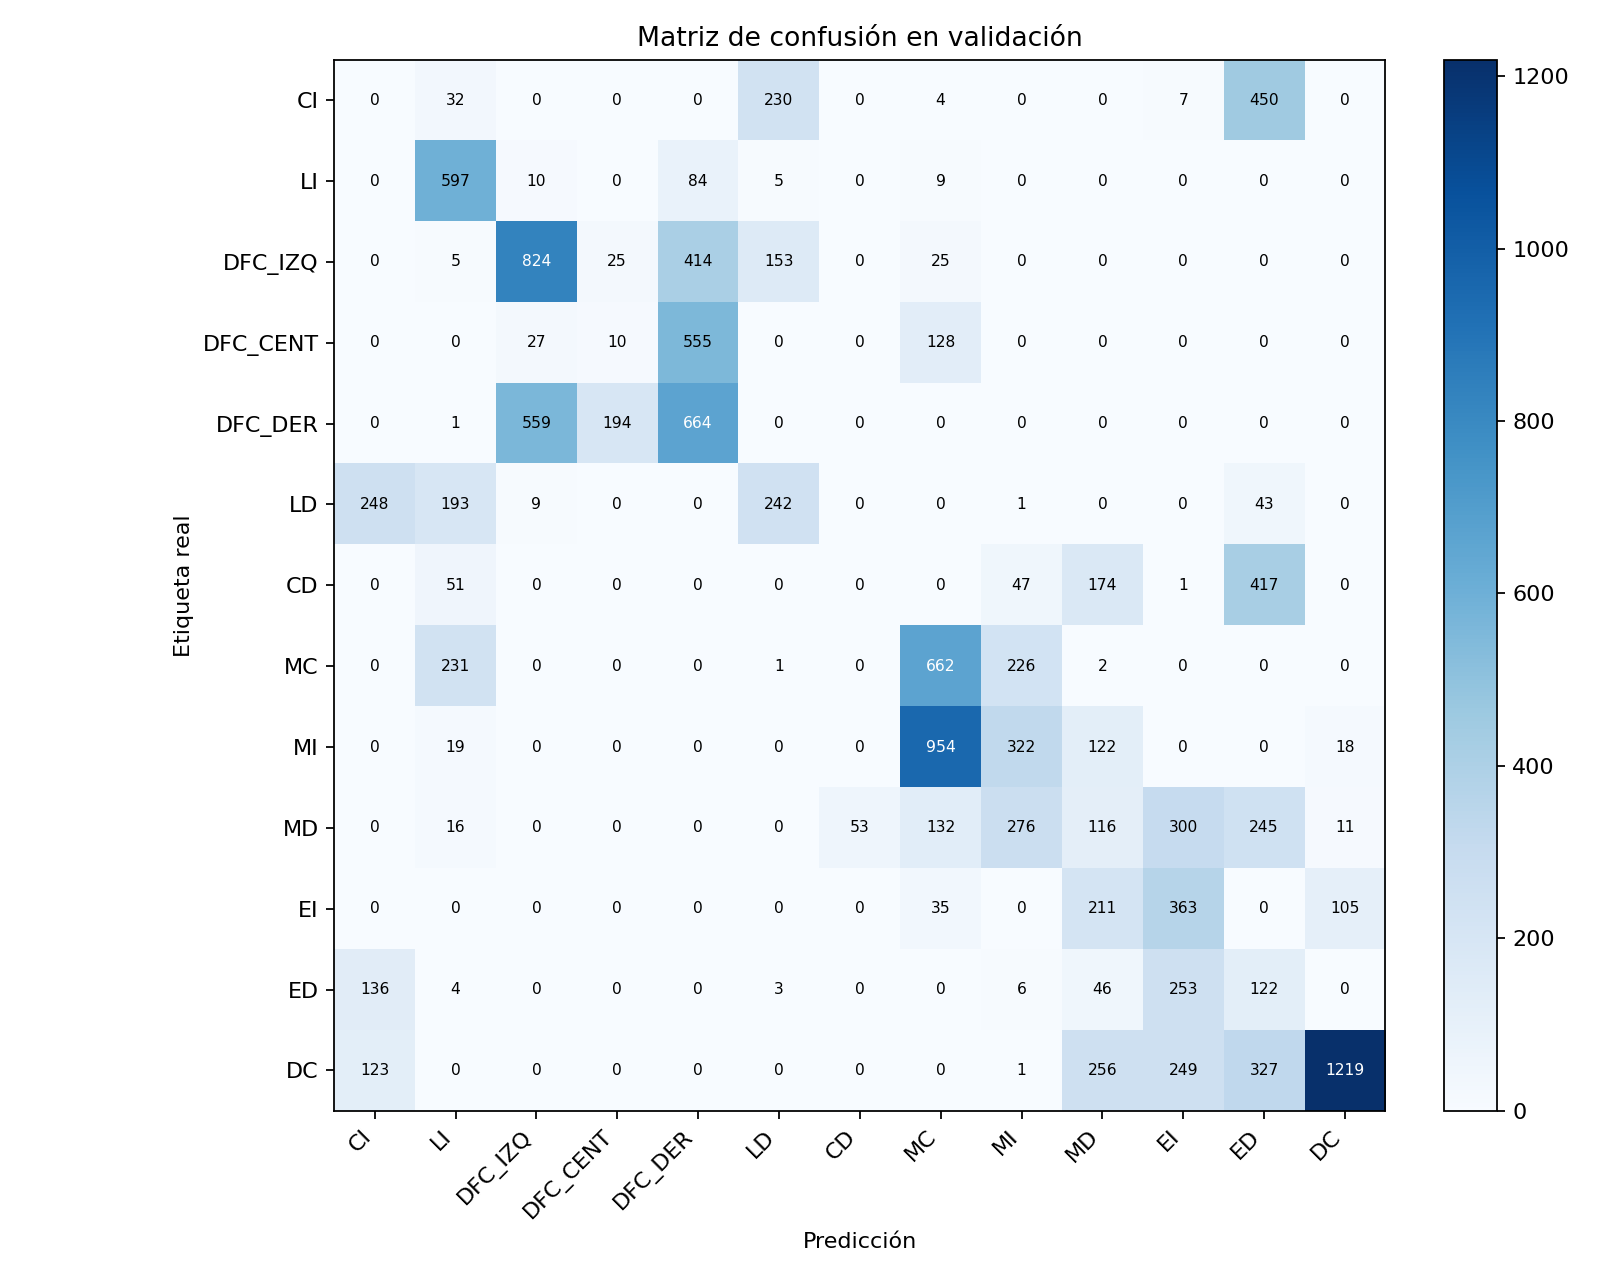
\includegraphics[width=0.8\linewidth]{Imagenes//Propias//matriz_confusion_grid_13.png}
\caption{Matriz de confusión en test del mejor modelo entrenado con 13 clases.}
\label{fig:confusion_grid_13}
\end{figure}


\subsubsection{Prueba 2: fusión de carrileros con laterales}

En la segunda prueba se mantuvo la mejor configuración de la Prueba 1 y se aplicó el mapeo:

\[
\texttt{CI} \rightarrow \texttt{LI},\quad \texttt{CD} \rightarrow \texttt{LD}
\]

El número de clases pasó de 13 a 11. Se puede observar en la \hyperref[tab:grid_merged_metrics]{Tabla~\ref*{tab:grid_merged_metrics}} y en la \hyperref[fig:confusion_merged]{Figura~\ref*{fig:confusion_merged}} que el rendimiento aumentó de forma clara, especialmente en validación (\(+0.2169\) en \textit{macro-F1}) y también en test (\(+0.0823\) en \textit{macro-F1}) respecto a la Prueba 1.

Esta prueba confirmó que, con el volumen de datos disponible, separar carrileros y laterales introducía más ruido que información útil.

\begin{table}[H]
\centering
\scriptsize
\begin{tabular}{c|c|c|c}
\textbf{Conjunto} & \textbf{Accuracy} & \textbf{Macro-F1} & \textbf{Weighted-F1} \\
\hline\hline
Validación & 0.5563 & 0.5265 & 0.5628 \\
\hline
Test & 0.5240 & 0.4845 & 0.5156 \\
\hline
\end{tabular}
\caption{Métricas tras fusionar carrileros con laterales.}
\label{tab:grid_merged_metrics}
\end{table}

\begin{figure}[H]
\centering
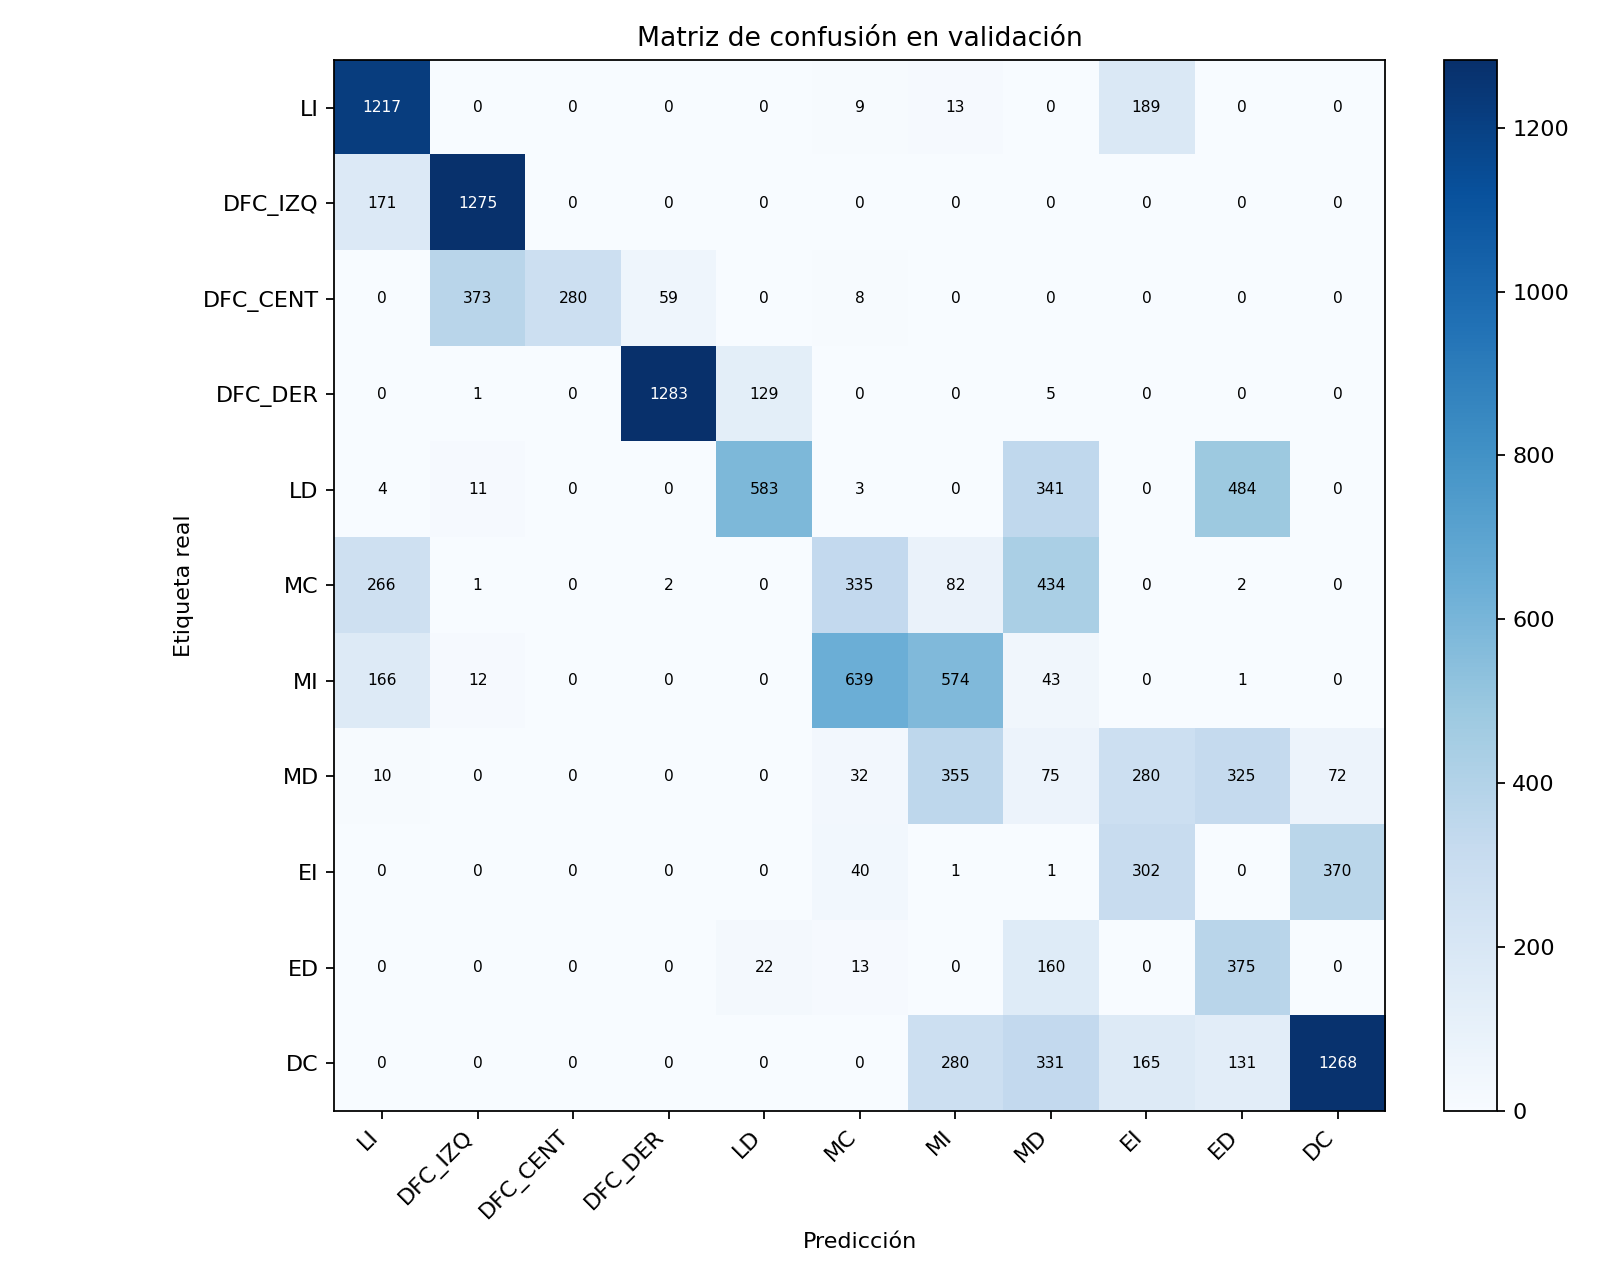
\includegraphics[width=0.8\linewidth]{Imagenes//Propias//matriz_confusion_carrileros_fusionados.png}
\caption{Matriz de confusión en test tras fusionar \texttt{CI} con \texttt{LI} y \texttt{CD} con \texttt{LD}.}
\label{fig:confusion_merged}
\end{figure}


\subsubsection{Prueba 3: grid search completo con 11 clases}

Tras comprobar que el mapeo era beneficioso, se repitió un grid search completo con 11 clases. Se exploraron de nuevo 480 combinaciones. La mejor configuración utilizó una arquitectura más compacta, 5 bloques de atención y mayor regularización.

La \hyperref[tab:grid_11_metrics]{Tabla~\ref*{tab:grid_11_metrics}} y la \hyperref[fig:confusion_grid_11]{Figura~\ref*{fig:confusion_grid_11}} resumen los resultados obtenidos. Aunque la validación mejoró claramente frente a la Prueba 2 (\(+0.0666\) en \textit{macro-F1}), el rendimiento en test apenas aumentó (\(+0.0048\) en \textit{macro-F1}). Esto sugiere que algunas configuraciones empezaban a adaptarse demasiado al clip de validación.

\begin{table}[H]
\centering
\scriptsize
\begin{tabular}{c|c|c|c}
\textbf{Conjunto} & \textbf{Accuracy} & \textbf{Macro-F1} & \textbf{Weighted-F1} \\
\hline\hline
Validación & 0.6168 & 0.5931 & 0.6207 \\
\hline
Test & 0.5170 & 0.4893 & 0.5096 \\
\hline
\end{tabular}
\caption{Métricas del grid search completo con 11 clases.}
\label{tab:grid_11_metrics}
\end{table}

\begin{figure}[H]
\centering
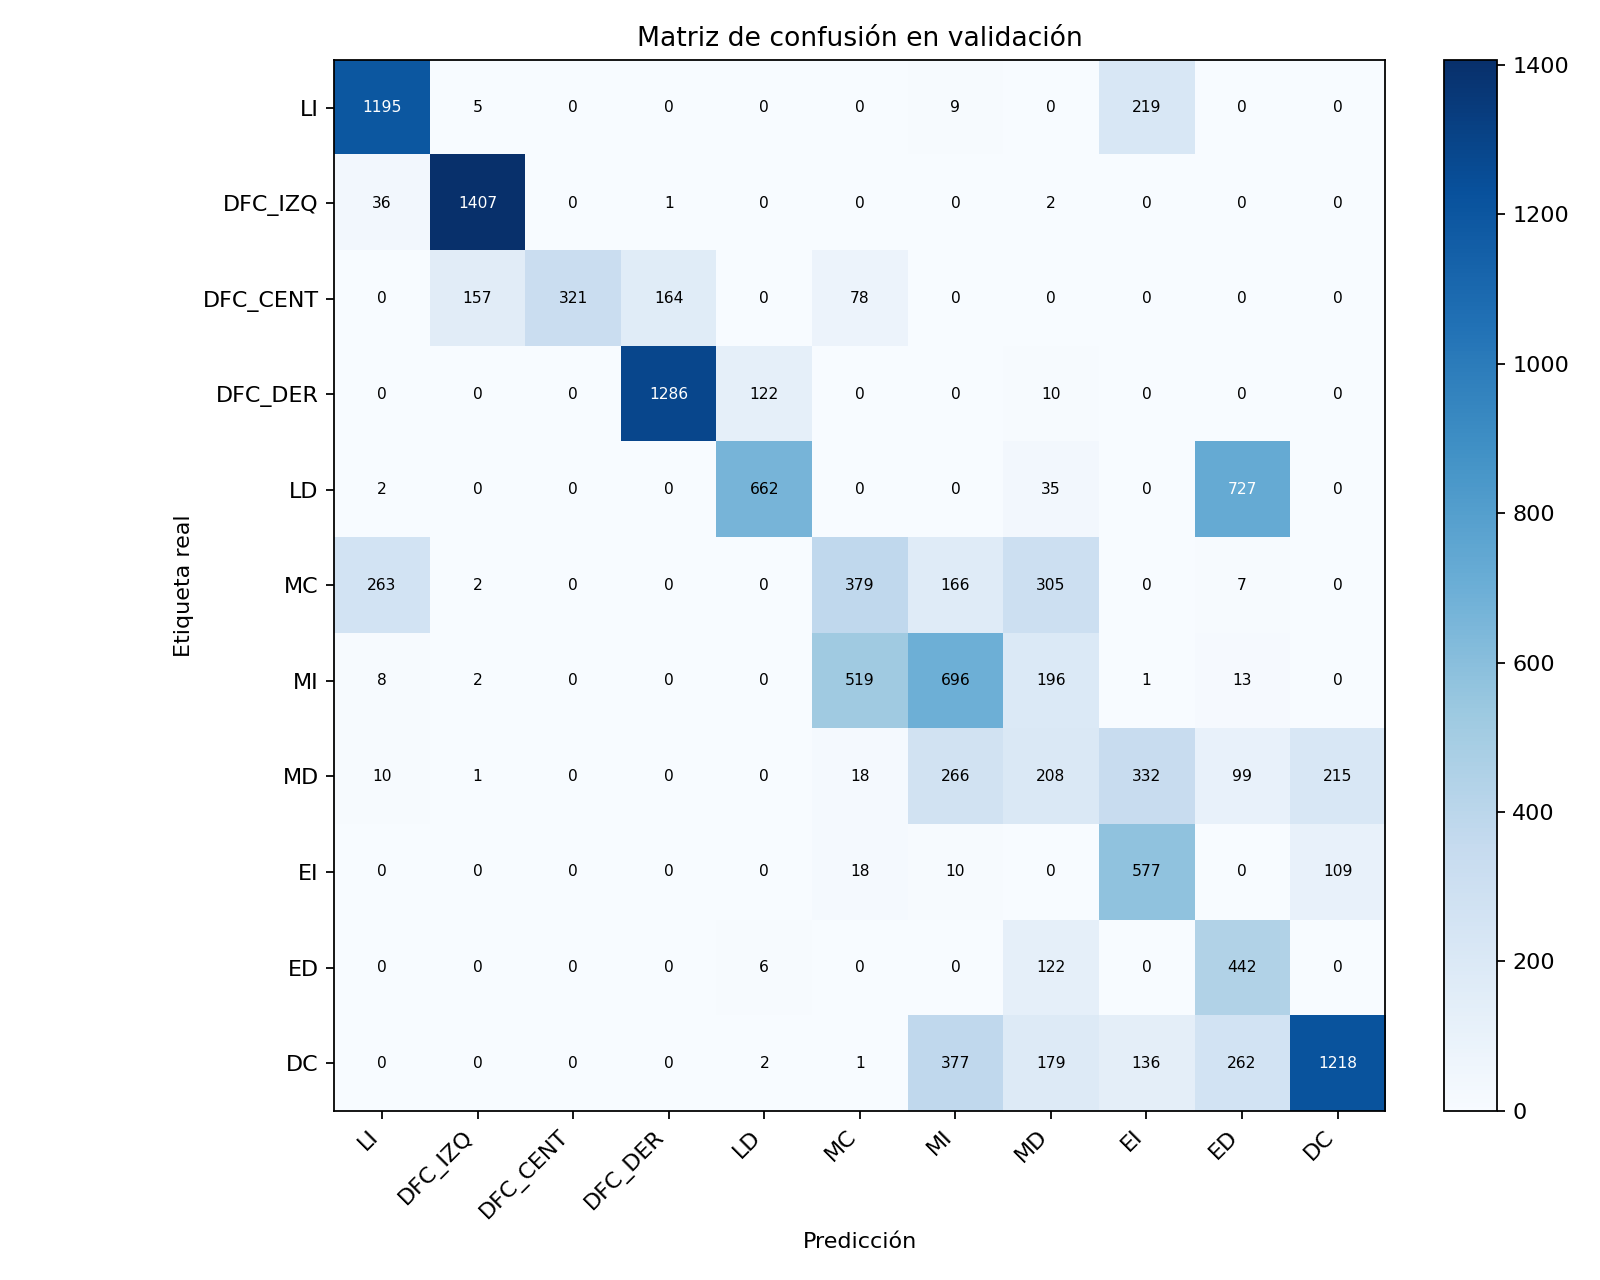
\includegraphics[width=0.8\linewidth]{Imagenes//Propias//matriz_confusion_grid_11.png}
\caption[Matriz de confusión del mejor modelo del grid search]{Matriz de confusión en test del mejor modelo del grid search completo con 11 clases.}
\label{fig:confusion_grid_11}
\end{figure}


\subsubsection{Prueba 4: refinamiento de los tres mejores modelos}

En la última fase se tomaron los tres mejores modelos del grid anterior y se refinó alrededor de ellos. En lugar de volver a cruzar todos los parámetros, se mantuvieron fijas tres familias arquitectónicas base y se probaron nuevos valores de \texttt{learning\_rate}, \texttt{weight\_decay}, \texttt{dropout} y \texttt{label\_smoothing}. Las tres arquitecturas base utilizadas se resumen en la \hyperref[tab:arquitecturas_refinamiento_posiciones]{Tabla~\ref*{tab:arquitecturas_refinamiento_posiciones}}.

\begin{table}[H]
\centering
\scriptsize
\begin{tabular}{c|c|c|c|c}
\textbf{Modelo} & \textbf{Perfil de anchura} & \texttt{objective\_num\_layers} & \texttt{ff\_expansion} & \texttt{num\_set\_blocks} \\
\hline\hline
1 & \((64,128,128,128)\) & \(2\) & \(4\) & \(5\) \\
\hline
2 & \((128,256,256,256)\) & \(1\) & \(2\) & \(5\) \\
\hline
3 & \((128,256,256,256)\) & \(1\) & \(2\) & \(3\) \\
\hline
\end{tabular}
\caption[Arquitecturas base del refinamiento]{Arquitecturas base utilizadas en la fase de refinamiento de hiperparámetros. El perfil de anchura se expresa como \((\texttt{teammate\_embed\_dim},\texttt{objective\_hidden\_dim},\texttt{set\_hidden\_dim},\texttt{fusion\_hidden\_dim})\).}
\label{tab:arquitecturas_refinamiento_posiciones}
\end{table}

En total se ejecutaron 108 entrenamientos.

El mejor modelo final obtuvo un \textit{macro-F1} de 0.6068 en validación y 0.5588 en test, como se muestra en la \hyperref[tab:modelo_final_metricas]{Tabla~\ref*{tab:modelo_final_metricas}}. La matriz de confusión en test se representa en la \hyperref[fig:confusion_modelo_final]{Figura~\ref*{fig:confusion_modelo_final}}.

\begin{table}[H]
\centering
\scriptsize
\begin{tabular}{c|c|c|c}
\textbf{Conjunto} & \textbf{Accuracy} & \textbf{Macro-F1} & \textbf{Weighted-F1} \\
\hline\hline
Validación & 0.6333 & 0.6068 & 0.6358 \\
\hline
Test & 0.5804 & 0.5588 & 0.5703 \\
\hline
\end{tabular}
\caption{Métricas del modelo final tras el refinamiento de hiperparámetros.}
\label{tab:modelo_final_metricas}
\end{table}

\begin{figure}[H]
\centering
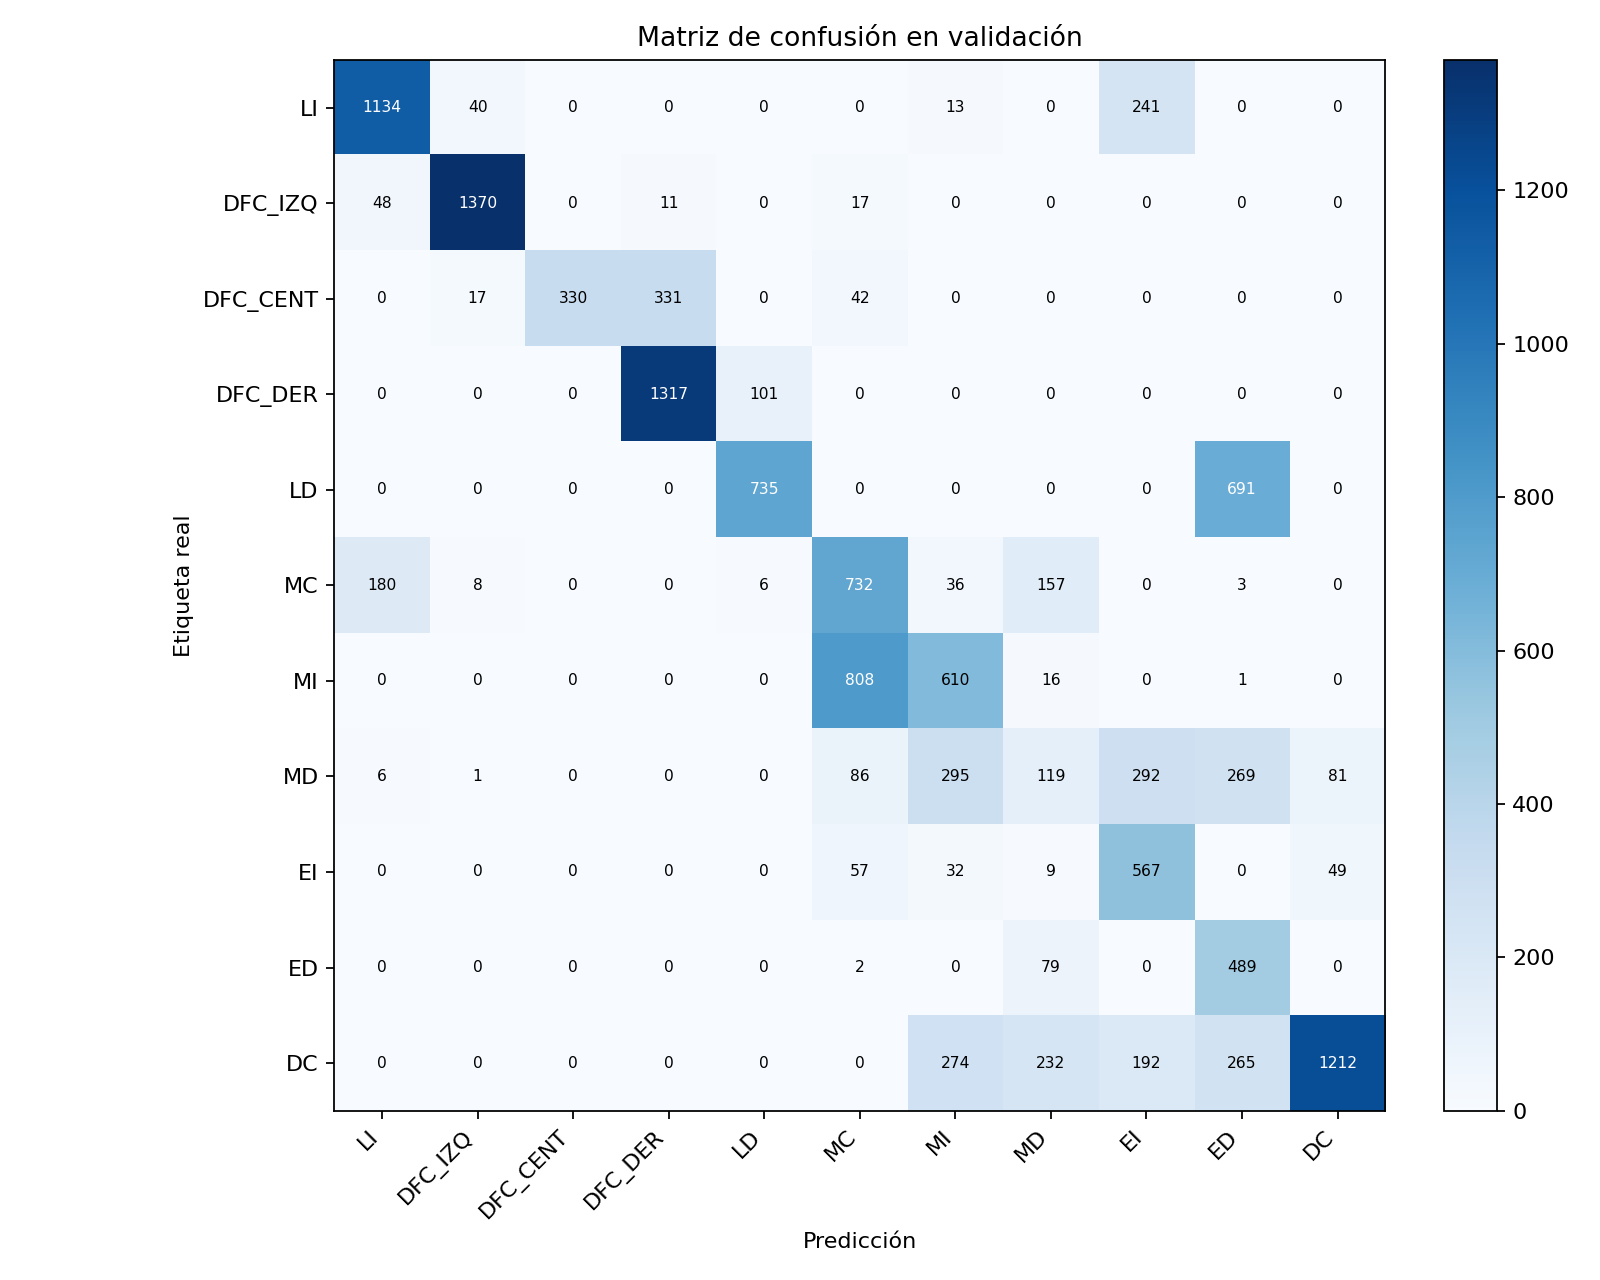
\includegraphics[width=0.8\linewidth]{Imagenes//Propias//matriz_confusion_modelo_final.png}
\caption{Matriz de confusión en test del modelo final.}
\label{fig:confusion_modelo_final}
\end{figure}

La curva de entrenamiento de la \hyperref[fig:curvas_entrenamiento_modelo_final]{Figura~\ref*{fig:curvas_entrenamiento_modelo_final}} muestra que el mejor punto se alcanza en las primeras épocas. A partir de ese momento, el rendimiento en entrenamiento sigue mejorando, pero la validación deja de mejorar de forma consistente. Este comportamiento indica sobreajuste temprano, algo esperable por la fuerte correlación entre frames de un mismo clip y por el tamaño limitado del conjunto de partidos etiquetados. Por ello se utiliza parada temprana y se selecciona el checkpoint con mayor \textit{macro-F1} de validación.

\begin{figure}[H]
\centering
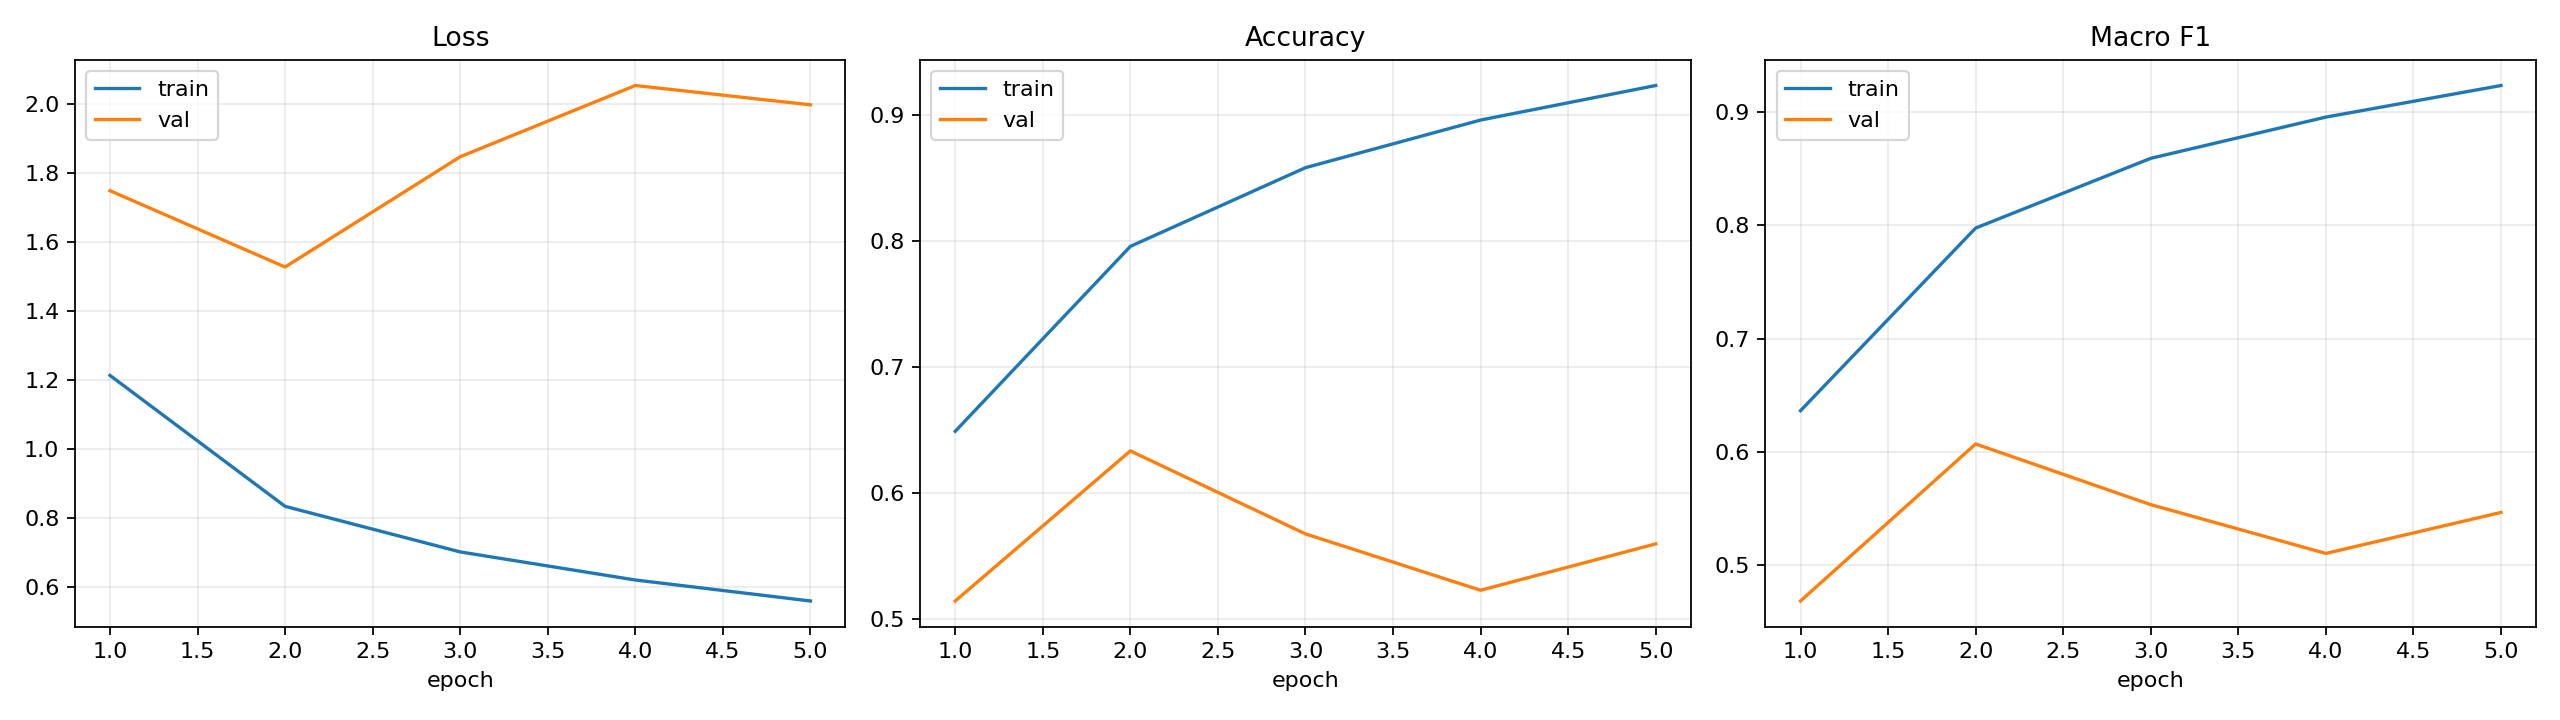
\includegraphics[width=0.49\linewidth]{Imagenes//Propias//curvas_entrenamiento_modelo_final.png}
\caption[Curvas entrenamiento del modelo final]{Evolución de la pérdida, accuracy y macro-F1 durante el entrenamiento del modelo final.}
\label{fig:curvas_entrenamiento_modelo_final}
\end{figure}


\subsection{Hiperparámetros del modelo final}
\label{subsec:hiperparametros-modelo-posicional}

El modelo final utiliza la siguiente configuración especificada en la \hyperref[tab:hiperparametros_modelo_final]{Tabla~\ref*{tab:hiperparametros_modelo_final}}:

\begin{table}[H]
\centering
\scriptsize
\begin{tabular}{c|c}
\textbf{Parámetro} & \textbf{Valor} \\
\hline\hline
\texttt{teammate\_embed\_dim} & 128 \\
\hline
\texttt{objective\_hidden\_dim} & 256 \\
\hline
\texttt{set\_hidden\_dim} & 256 \\
\hline
\texttt{fusion\_hidden\_dim} & 256 \\
\hline
\texttt{objective\_num\_layers} & 1 \\
\hline
\texttt{num\_set\_blocks} & 5 \\
\hline
\texttt{num\_heads} & 4 \\
\hline
\texttt{ff\_expansion} & 2 \\
\hline
\texttt{dropout} & 0.27 \\
\hline
\texttt{label\_smoothing} & 0.05 \\
\hline
\texttt{learning\_rate} & 0.0002 \\
\hline
\texttt{weight\_decay} & 0.0015 \\
\hline
\texttt{batch\_size} & 512 \\
\hline
\end{tabular}
\caption{Hiperparámetros del modelo final.}
\label{tab:hiperparametros_modelo_final}
\end{table}

El parámetro \texttt{teammate\_embed\_dim} controla la anchura de la MLP que codifica cada compañero antes de introducirlo en la atención. El parámetro \texttt{objective\_hidden\_dim} define la dimensión oculta usada para representar al jugador objetivo.

Por otro lado, \texttt{set\_hidden\_dim} es la dimensión interna del Set Transformer. Es uno de los valores más importantes, ya que determina la capacidad del modelo para representar relaciones entre compañeros. \texttt{fusion\_hidden\_dim} define la anchura del clasificador final tras concatenar el embedding del jugador objetivo y el resumen del conjunto.

El parámetro \texttt{objective\_num\_layers} indica cuántas capas ocultas tiene la MLP del jugador objetivo. En el modelo final se usa una única capa, lo que sugiere que las variables individuales son suficientemente expresivas y que añadir más profundidad aumentaba el riesgo de sobreajuste.

El número de bloques de auto-atención que se aplican sobre los compañeros está definido por \texttt{num\_set\_blocks}. El modelo final usa 5 bloques, permitiendo refinar varias veces las relaciones espaciales del conjunto. \texttt{num\_heads} indica el número de cabezas de atención en paralelo. Con 4 cabezas, el modelo puede aprender distintos tipos de relaciones tácticas simultáneamente.

Para controlar cuánto se expande la dimensión interna dentro del bloque \textit{feed-forward} de cada bloque de atención se utiliza \texttt{ff\_expansion}. \texttt{dropout} introduce regularización apagando aleatoriamente neuronas durante el entrenamiento. El valor final, 0.27, es relativamente alto, coherente con el sobreajuste observado.

Con \texttt{label\_smoothing} se suavizan las etiquetas durante el entrenamiento. En vez de asignar probabilidad 1 a la clase correcta y 0 al resto, reparte una pequeña fracción de probabilidad entre las demás clases. Esto es útil porque algunas posiciones son tácticamente ambiguas.

Por último, \texttt{learning\_rate} controla el tamaño de los pasos del optimizador, y \texttt{weight\_decay} penaliza pesos demasiado grandes. Ambos contribuyen a estabilizar el entrenamiento y mejorar la generalización.

\subsection{Resultados por clase}
\label{subsec:resultados-clase-posicional}

El modelo final alcanza una accuracy de 0.5804 y un \textit{macro-F1} de 0.5588 en test. En la \hyperref[tab:set_transformer_test_by_class]{Tabla~\ref*{tab:set_transformer_test_by_class}} se puede observar que las mejores clases son \texttt{DFC\_IZQ}, \texttt{ED}, \texttt{DFC\_DER}, \texttt{DC} y \texttt{LI}. Las clases más difíciles son \texttt{DFC\_CENT}, \texttt{MD}, \texttt{MC} y \texttt{MI}.

\begin{table}[H]
\centering
\scriptsize
\begin{tabular}{c|c|c|c|c}
\textbf{Clase} & \textbf{Precisión test} & \textbf{Recall test} & \textbf{F1 test} & \textbf{Soporte test} \\
\hline\hline
\texttt{LI} & 0.6078 & 0.5985 & 0.6031 & 1432 \\
\hline
\texttt{DFC\_IZQ} & 0.9026 & 0.8560 & 0.8787 & 1451 \\
\hline
\texttt{DFC\_CENT} & 0.6272 & 0.1434 & 0.2335 & 739 \\
\hline
\texttt{DFC\_DER} & 0.5910 & 0.6723 & 0.6290 & 1367 \\
\hline
\texttt{LD} & 0.5820 & 0.5363 & 0.5582 & 1337 \\
\hline
\texttt{MC} & 0.4194 & 0.4783 & 0.4469 & 1403 \\
\hline
\texttt{MI} & 0.4724 & 0.4823 & 0.4773 & 1188 \\
\hline
\texttt{MD} & 0.4848 & 0.3457 & 0.4036 & 1478 \\
\hline
\texttt{EI} & 0.4263 & 0.9294 & 0.5845 & 694 \\
\hline
\texttt{ED} & 0.5464 & 0.9874 & 0.7035 & 715 \\
\hline
\texttt{DC} & 0.7674 & 0.5322 & 0.6285 & 1990 \\
\hline
\end{tabular}
\caption{Resultados por clase del modelo final sobre el conjunto de test.}
\label{tab:set_transformer_test_by_class}
\end{table}

Estos resultados son coherentes con la naturaleza de la tarea. Las posiciones de banda y algunos defensas tienen patrones espaciales más estables, mientras que los mediocentros e interiores dependen más de la fase de juego, de intercambios posicionales y del contexto colectivo.

\subsection{Reentrenamiento con \textit{train+val}}
\label{subsec:reentrenamiento-train-val-posicional}

Una vez seleccionado el mejor modelo mediante el \textit{grid search}, se realizó una prueba adicional para comprobar si el rendimiento podía mejorar utilizando más datos durante el entrenamiento. La idea consistía en unir los conjuntos de entrenamiento y validación, entrenar de nuevo el modelo con los hiperparámetros previamente seleccionados y evaluar el resultado únicamente sobre el conjunto de test. Esta prueba tiene sentido porque el modelo mostraba síntomas de sobreajuste temprano, por lo que cabía pensar que disponer de más muestras durante el entrenamiento podría mejorar su capacidad de generalización.

En esta prueba se entrenó el modelo durante 2 épocas, que era la época óptima obtenida en el proceso de validación anterior. El conjunto \textit{train+val} contenía 95725 muestras, mientras que el conjunto de test se mantuvo separado y no se utilizó para tomar decisiones durante el entrenamiento.

Como se observa en la \hyperref[tab:comparacion_train_val_posiciones]{Tabla~\ref*{tab:comparacion_train_val_posiciones}}, el reentrenamiento con \textit{train+val} no mejoró los resultados en test. Aunque el modelo alcanzó sobre \textit{train+val} una \textit{accuracy} de 0.8890 y un \textit{macro-F1} de 0.8924, su rendimiento sobre test fue inferior al del modelo seleccionado mediante validación. Esto indica que añadir la partición de validación al entrenamiento no redujo el sobreajuste, sino que probablemente aumentó la adaptación del modelo a los fragmentos ya vistos. En este caso, todos los vídeos etiquetados proceden del mismo partido, por lo que la caída no se debe a un cambio completo de dominio entre partidos distintos. Por este motivo, se decidió mantener como modelo principal el seleccionado mediante validación, ya que ofrecía una mejor generalización sobre el fragmento reservado como test.

\begin{table}[H]
    \centering
    \scriptsize
    \begin{tabular}{p{0.36\linewidth}|c|c|c}
        \textbf{Modelo} & \textbf{Acc. test} & \textbf{Macro-F1 test} & \textbf{Weighted-F1 test} \\
        \hline\hline
        Modelo seleccionado por validación & 0.5804 & 0.5588 & 0.5703 \\
        \hline
        Reentrenado con \textit{train+val} & 0.5161 & 0.4833 & 0.5020 \\
        \hline
    \end{tabular}
    \caption[Comparación de estrategias de entrenamiento]{Comparación entre el modelo seleccionado en validación y el modelo reentrenado con \textit{train+val}.}
    \label{tab:comparacion_train_val_posiciones}
\end{table}


\subsection{Asignación táctica final de posiciones}
\label{subsec:asignacion-tactica-final-posiciones}

Tras obtener las probabilidades del Set Transformer, la inferencia no termina escogiendo simplemente la clase con mayor probabilidad para cada jugador. Esa predicción directa existe, pero se utiliza únicamente como una primera estimación. Posteriormente se aplica una fase de asignación táctica cuyo objetivo es que las posiciones finales sean coherentes con la alineación esperada de cada equipo.

Para ello, el flujo combina dos niveles de asignación: una asignación inmediata por frame y una reasignación estable por segmentos temporales de identidad.

\subsubsection{Asignación online por frame}

En cada frame, el modelo recibe como entrada los tracks activos generados en las fases previas del pipeline. Para cada track correspondiente a un jugador de campo, se construye una muestra formada por dos bloques de información: por un lado, las 14 variables propias del jugador, descritas en la \hyperref[subsec:variables-inferencia-posicional]{Sección~\ref*{subsec:variables-inferencia-posicional}}, y por otro, una matriz de contexto de tamaño \(10 \times 11\), que representa hasta 10 compañeros del mismo equipo mediante 11 variables por compañero.

Una vez construida esta representación $x_i$, la muestra se introduce en el Set Transformer descrito en las secciones anteriores. El modelo devuelve, para cada track, un vector de logits asociado a las clases posicionales aprendidas. Estos logits se transforman posteriormente en probabilidades mediante la función \textit{softmax}, obteniendo así una estimación de pertenencia del jugador a cada una de las posiciones posibles. La predicción de rol de cada jugador se obtiene mediante la clase con mayor probabilidad:

\[
\hat{y}_i = \arg\max_{c \in \mathcal{C}} p_i(c)
\]

Sin embargo, esta predicción no constituye todavía la posición final de cada jugador. El Set Transformer proporciona una estimación probabilística inicial para cada una de las 11 clases aprendidas (\texttt{LI}, \texttt{DFC\_IZQ}, \texttt{DFC\_CENT}, \texttt{DFC\_DER}, \texttt{LD}, \texttt{MC}, \texttt{MI}, \texttt{MD}, \texttt{EI}, \texttt{ED}, \texttt{DC}), pero después se aplica una fase de asignación táctica cuyo objetivo es que las posiciones finales sean coherentes con la alineación esperada de cada equipo. Este paso evita configuraciones tácticamente imposibles; por ejemplo, que varios jugadores queden asignados simultáneamente como delanteros mientras otras plazas defensivas del once esperado quedan vacías.

Para realizar esta corrección se construye una matriz de costes entre los tracks activos y las plazas tácticas esperadas en la alineación. Cada fila de la matriz representa un track detectado en el frame y cada columna representa una plaza del once esperado. Por ejemplo, si una formación contiene dos delanteros, existirán dos columnas distintas asociadas a la clase \texttt{DC}.

El coste entre el track \(i\) y la plaza táctica \(j\) se calcula a partir de la probabilidad que el modelo asigna a la clase correspondiente para dicho track y penalizaciones relacionadas con la familia espacial y la posición en el campo. De forma simplificada, puede expresarse como:

\[
C_{ij}=\min_{\ell\in A(s_j)}
\left[
-\log\left(p_i(\ell)+\varepsilon\right)
+\mathrm{pen}_{\mathrm{compat}}(s_j,\ell)
+\mathrm{pen}_{\mathrm{geo}}(i,s_j)
\right]
\]


donde \(s_j\) es la clase posicional asociada a la plaza \(j\), \(A(s_j)\) es el conjunto de etiquetas del modelo compatibles con esa plaza \(s_j\), \(\ell\) es una etiqueta candidata dentro del conjunto \(A(s_j)\), \(p_i(\ell)\) es la probabilidad asignada por el modelo al track \(i\) para la etiqueta \(\ell\), y \(\varepsilon\) es un valor pequeño para evitar el logaritmo de cero. De este modo, una probabilidad alta produce un coste bajo, mientras que una probabilidad baja produce un coste alto.

En esta implementación solo se relaja la compatibilidad en las posiciones de banda. 
Para ello se definen dos familias laterales:
\[
\mathcal{B}_{\mathrm{izq}}=\{\texttt{LI},\texttt{MI},\texttt{EI}\},
\qquad
\mathcal{B}_{\mathrm{der}}=\{\texttt{LD},\texttt{MD},\texttt{ED}\}.
\]

El conjunto de etiquetas compatibles con una plaza \(s\) se define como:
\[
A(s)=
\begin{cases}
\mathcal{B}_{\mathrm{izq}}, & \text{si } s\in \mathcal{B}_{\mathrm{izq}},\\[0.3em]
\mathcal{B}_{\mathrm{der}}, & \text{si } s\in \mathcal{B}_{\mathrm{der}},\\[0.3em]
\{s\}, & \text{en otro caso}.
\end{cases}
\]

La penalización de compatibilidad entre plaza y etiqueta se define como:
\[
\mathrm{pen}_{\mathrm{compat}}(s,\ell)=
\begin{cases}
0 & s=\ell,\\
0 & \text{si } \mathrm{fam}(s)=\varnothing \ \text{o}\ \mathrm{fam}(\ell)=\varnothing,\\
1000 & \text{si } \mathrm{fam}(s)\neq \mathrm{fam}(\ell),\\
0.35 & \text{si } \mathrm{fam}(s)=\mathrm{fam}(\ell)\ \text{y falta alguna ancla},\\
\lambda_{\mathrm{compat}}\, d_{\mathrm{anch}}(a_s,a_\ell) & \text{si } \mathrm{fam}(s)=\mathrm{fam}(\ell)\ \text{con anclas disponibles},
\end{cases}
\]
donde \(\mathrm{fam}(\cdot)\in\{\texttt{LEFT},\texttt{RIGHT},\varnothing\}\) denota la familia lateral del rol
(\(\varnothing\) para roles sin familia lateral), y en esta implementación \(\lambda_{\mathrm{compat}}=1.10\).

La penalización geométrica se define como:
\[
\mathrm{pen}_{\mathrm{geo}}(i,s)=\lambda_{\mathrm{geo}}\; d_{\mathrm{anch}}\big((x_i,y_i),a_s\big),
\]
donde \((x_i,y_i)\) es la posición normalizada del track \(i\), \(a_s\) es el ancla táctica de la plaza \(s\), y \(\lambda_{\mathrm{geo}}\) es el peso geométrico.
donde \((x_i,y_i)\) es la posición normalizada del track \(i\), \(a_s\) es el ancla táctica de la plaza \(s\), y \(\lambda_{\mathrm{geo}}\) es el peso geométrico (en esta implementación, \(\lambda_{\mathrm{geo}}=1.35\)). Este parámetro controla cuánto influye la coherencia espacial en el coste total: valores más altos penalizan con mayor intensidad los emparejamientos alejados de su ancla táctica, mientras que valores más bajos priorizan en mayor medida la probabilidad del modelo.

La distancia ponderada a ancla utilizada en ambos términos es:
\[
d_{\mathrm{anch}}(u,v)=\sqrt{(u_x-v_x)^2+\left(\alpha_y\,(u_y-v_y)\right)^2},
\]
con \(\alpha_y\) como factor de ponderación vertical (en esta implementación, \(\alpha_y=1.20\)), de modo que diferencias en el eje \(y\), es decir sobr el eje del ancho del campo, se penalizan ligeramente más que diferencias equivalentes en \(x\).

Una vez construida la matriz de costes \(C\), se aplica el algoritmo húngaro para obtener la asignación global $\sigma^*$ de menor coste entre tracks y plazas tácticas:

\[
\sigma^* =
\arg\min_{\sigma}
\sum_i C_{i,\sigma(i)}
\]

donde \(\sigma(i)\) indica la plaza asignada al track \(i\). El algoritmo debe cumplir además que una misma plaza táctica no pueda ser asignada a dos tracks distintos. Esta optimización no toma decisiones de forma independiente para cada jugador, sino que busca una solución conjunta para todo el equipo. Por ejemplo, aunque varios tracks tengan alta probabilidad de pertenecer a la clase \texttt{DC}, el algoritmo solo podrá asignarlos a plazas de delantero si esas plazas existen realmente en el once esperado. El resultado final es una asignación de roles coherente con la alineación introducida.


\subsubsection{Apertura y cierre de segmentos}
\label{subsec:aperturaSegmentos}

La estabilidad temporal se organiza mediante segmentos de identidad. Esta decisión está motivada por el objetivo final de la inferencia posicional: no se busca únicamente estimar la posición táctica de un jugador en un frame concreto, sino utilizar esa posición para asociar el track con el futbolista real de la alineación. Dado que se dispone del once inicial, si se infiere de forma estable que un jugador ocupa una determinada plaza táctica, es posible asociarlo con el nombre correspondiente en la alineación introducida.

Idealmente, un track representaría una única identidad durante toda su vida. En ese caso, bastaría con inferir su posición una vez, o acumular evidencia a lo largo del track completo, para asignarle un jugador real. Sin embargo, en la práctica el tracking puede sufrir pérdidas, reasociaciones o cambios de identidad. Por tanto, no se puede asumir que un mismo \textit{track id} corresponda siempre al mismo futbolista durante todo el vídeo.

Por este motivo, en lugar de tratar cada track como una identidad indivisible, su vida temporal se divide en segmentos. Un segmento representa un tramo continuo del track en el que el sistema considera razonable acumular evidencia para una misma identidad táctica. Mientras no aparezcan señales fuertes de ruptura, las nuevas asignaciones se siguen incorporando al segmento activo.

La apertura de un nuevo segmento se activa en dos tipos de situaciones. La primera corresponde a casos en los que el ByteTrack no conservó la identidad temporal, y fue posteriormente la capa canónica de tracking, quién reasoció esa identidad. La segunda aparece cuando se detecta un salto posicional grande acompañado también de un cambio de rol respecto al rol dominante acumulado en el segmento. En estos casos, el segmento anterior se cierra, se almacena su estado agregado y se abre un nuevo segmento vacío para empezar a acumular evidencia desde ese punto.

De esta forma, un track no define necesariamente una única identidad final. En su lugar, son sus segmentos los que actúan como unidades temporales de identidad. Cada segmento acumula su propia evidencia posicional y puede asociarse posteriormente con una plaza táctica de la alineación. Este mecanismo evita mezclar en una misma memoria temporal observaciones que podrían pertenecer a futbolistas distintos o a tramos del track cuya continuidad no es completamente fiable.

\subsubsection{Acumulación de evidencia por segmento}

Una vez definido el segmento activo de cada track, el sistema acumula sobre él las asignaciones obtenidas frame a frame tras aplicar la corrección táctica mediante el algoritmo húngaro. Por tanto, la identidad táctica de un segmento no se decide a partir de una única predicción aislada, sino a partir del conjunto de evidencias recogidas durante su duración.

Para cada segmento activo se almacenan distintas estadísticas: el número de observaciones, los conteos de votos por rol, la suma de confianzas asociadas a cada rol, el rol dominante en el histórico del segmento, el rol dominante en una ventana temporal reciente y estadísticas espaciales resumidas del jugador.

Además de los votos categóricos, el sistema conserva información sobre la posición media del jugador en el campo, sus posiciones recientes y la última posición válida observada para poder determinar la continuidad o cierre del segmento, como se explica en la sección anterior.

\subsubsection{Reasignación estable por segmentos}

Una vez acumulada evidencia sobre los segmentos activos, se aplica un segundo nivel de asignación táctica. A diferencia de la asignación online por frame, esta reasignación no trabaja con predicciones instantáneas de tracks, sino con segmentos temporales que resumen la evidencia recogida durante varios frames.

Para cada equipo se construye una nueva matriz de costes entre los segmentos activos y las plazas tácticas del once esperado. Cada fila representa un segmento y cada columna una plaza de la alineación. El coste entre un segmento \(i\) y una plaza táctica \(j\) combina tres fuentes de información: la frecuencia con la que el segmento ha sido asignado al rol asociado a esa plaza, la confianza acumulada en dichas asignaciones y la coherencia geométrica entre la posición media del segmento y el ancla táctica de la plaza.

De forma simplificada, este coste puede expresarse como:

\[
C^{seg}_{ij}
=
\left(1-\frac{n_i(s_j)}{N_i}\right)
-
\lambda_{conf}\,\bar{q}_i(s_j)
+
\lambda_{geo}\,d(\mu_i,a_j)
\]

donde \(s_j\) es el el rol de la plaza \(j\), \(n_i(s_j)\) es el número de votos del segmento \(i\) para ese \textit{slot}, \(N_i\) es el total de observaciones del segmento, \(\bar{q}_i(s_j)\) es la confianza media acumulada de esos votos, \(\mu_i\) es la posición media del segmento y \(a_j\) el ancla táctica de la plaza.

Sobre esta matriz se aplica de nuevo el algoritmo húngaro, obteniendo una asignación global de segmentos a plazas tácticas. Esta asignación se interpreta como el rol estable del segmento, ya que no depende de una única predicción del modelo, sino del conjunto de votos acumulados durante la vida del segmento.

En algunas alineaciones, además, existen plazas duplicadas que el modelo base no distingue como clases separadas. Por ejemplo, el modelo predice \texttt{DC} como clase única, pero el once esperado puede requerir dos plazas diferenciadas (\texttt{DC\_IZQ} y \texttt{DC\_DCHO}), De forma análoga puede ocurrir con \texttt{MC}. Para resolver esta desambiguación lateral, cada segmento mantiene un histórico de su relación espacial con ambas bandas (distancia acumulada a banda izquierda y a banda derecha). Cuando dos segmentos compiten por una pareja duplicada de una misma clase base, ese histórico lateral se utiliza para decidir cuál ocupa la plaza izquierda y cuál la derecha, obteniendo una asignación final más estable y tácticamente interpretable.

\subsubsection{Salida final y trazabilidad}

La salida final conserva información de los distintos niveles de inferencia. Por un lado, se mantiene la predicción instantánea del modelo para el frame actual; por otro, la asignación corregida por el algoritmo húngaro a nivel de frame; y, finalmente, la asignación estable obtenida tras acumular evidencia en el segmento.

\section{Clasificación de acciones}
\label{sec:clasificacion-acciones}

Una vez finalizada la fase de identificación de jugadores (quién), continuamos con la
fase de identificación de acciones (qué). Mientras que el tracking asigna identidades,
equipos y posiciones a cada jugador a lo largo del vídeo, la clasificación de acciones
se encarga de transformar esas trayectorias en eventos semánticos: pases, controles,
robos, tiros, saques y otras situaciones narrables del partido. Como se anticipó en la \hyperref[sec:pathcrf-tecnologias]{Sección~\ref*{sec:pathcrf-tecnologias}}, para esta tarea se ha integrado PathCRF, un modelo que formula la detección de eventos futbolísticos como una selección secuencial de aristas sobre un grafo dinámico de jugadores. En lugar de trabajar directamente sobre los frames de vídeo, PathCRF opera sobre las trayectorias (x, y) de los jugadores en el campo, lo que lo hace especialmente compatible con la salida del sistema de tracking desarrollado en las fases anteriores. Esta sección describe el proceso completo: desde la adaptación de los tracks al formato requerido por el modelo hasta la generación de eventos listos para ser narrados.


\subsection{Adaptación de tracks al formato PathCRF}
La entrada de esta fase no es el vídeo original, sino la salida estructurada de las fases anteriores: jugadores, porteros y árbitros ya identificados, asociados a equipos y proyectados al sistema de coordenadas del campo. A partir de esta información se construye una representación temporal compatible con PathCRF.

Esta representación adopta la forma de una tabla temporal en la que cada fila corresponde a un frame y cada columna describe el estado de uno de los actores del juego. Para cada jugador se incluyen sus coordenadas sobre el campo y variables de movimiento derivadas, como velocidad y aceleración. 

\subsubsection{Estabilidad de identidades}

Un requisito importante de esta transformación es que cada jugador ocupe un slot coherente a lo largo del tiempo. En la práctica, esta condición no se resuelve de nuevo dentro de la propia fase de acciones, sino que se apoya en la canonización ya realizada previamente por el tracking. Es decir, la fase de clasificación de acciones hereda una estructura de identidades ya estabilizada que se asume como válida y se reutiliza como base para construir la entrada del modelo.

En concreto, la representación se organiza en slots fijos separados por rol y por equipo: \texttt{home\_1} y \texttt{away\_1} para los porteros; \texttt{home\_2} a \texttt{home\_11} para los diez jugadores de campo del equipo local, \texttt{away\_2} a \texttt{away\_11} para los diez jugadores de campo del equipo visitante, y \texttt{referee\_1} a \texttt{referee\_3} para los árbitros.

\subsubsection{Relleno de observaciones ausentes}
En muchos frames no todos los slots tienen una detección asociada. PathCRF necesita disponer de una posición para cada slot en cada instante, por lo que los huecos deben rellenarse. La estrategia consiste en dos pasos: primero se interpola linealmente entre las posiciones conocidas de cada slot, recortando los valores extrapolados a los límites del terreno de juego (105 m × 68 m). Después, cuando un slot carece por completo de observaciones durante un tramo del vídeo, se utiliza una plantilla de equipo alineada con el centroide de los jugadores visibles en ese instante. Esta plantilla sitúa a los jugadores en una formación de referencia (aproximadamente un 4-2-3-1) que se desplaza y rota para seguir la posición media del equipo.

\subsubsection{Suavizado de trayectorias}
Antes de lanzar la inferencia, las trayectorias se suavizan para amortiguar pequeñas oscilaciones debidas al ruido acumulado de las fases previas. Aunque el tracking canónico ya proporciona identidades estables y posiciones proyectadas al campo, la localización de cada jugador sigue estando afectada por varios factores: imprecisión del detector, pequeñas variaciones en las \textit{bounding boxes}, errores de la homografía al proyectar desde la imagen broadcast al plano métrico del terreno de juego y desapariciones momentáneas por oclusión o cambio de plano. Como consecuencia, una trayectoria que en realidad debería ser suave puede presentar pequeños saltos laterales o aceleraciones entre frames consecutivos.

Este problema es especialmente importante en esta fase porque PathCRF no solo observa posiciones, sino también relaciones temporales entre jugadores. Si una trayectoria contiene jitter, el modelo puede interpretar incorrectamente que un jugador ha frenado bruscamente o que ha cambiado de dirección de forma repentina.

Para reducir este efecto, se aplica un preprocesado temporal en dos pasadas consecutivas. En cada pasada se detectan y corrigen \textit{outliers} aislados de movimiento: si los saltos \(t-1 \rightarrow t\) y \(t \rightarrow t+1\) superan el desplazamiento máximo permitido, pero el puente directo \(t-1 \rightarrow t+1\) sí es plausible, el punto intermedio \(t\) se sustituye por una interpolación entre sus vecinos. Después se aplica un suavizado mediante mediana móvil con ventana de 9 frames, un filtro Savitzky-Golay (11, orden 2) y un suavizado exponencial (\(\alpha = 0.35\)). Por último, se limita el jitter por paso, acotando el desplazamiento máximo entre frames al 75\% del umbral físico permitido.

Una vez estabilizadas las coordenadas, se recalculan las magnitudes cinemáticas de entrada al modelo (\(v_x\), \(v_y\), velocidad y aceleración) mediante diferencias finitas.

La finalidad de este preprocesado no es alterar el comportamiento global de los jugadores, sino eliminar irregularidades locales que podrían degradar la detección de eventos. En una tarea basada en relaciones temporales, pequeñas vibraciones frame a frame pueden traducirse fácilmente en falsos cambios de estado si no se corrigen previamente.

\subsection{Modelo PathCRF}
El núcleo de la fase de acciones es PathCRF, un modelo que combina una red de atención espacio-temporal con un campo aleatorio condicional (CRF) dinámico. Aunque esta arquitectura ya se describió en la \hyperref[sec:pathcrf-tecnologias]{Sección~\ref*{sec:pathcrf-tecnologias}}, conviene recordar los puntos clave del diseño.

\subsubsection{Arquitectura}
PathCRF representa el partido como un grafo completamente conectado que evoluciona en el tiempo . En cada instante \(t\), los nodos representan a los jugadores, junto con nodos externos asociados a salidas del campo (\texttt{out\_left}, \texttt{out\_right}, \texttt{out\_top}, \texttt{out\_bottom}). 

Las aristas dirigidas entre nodos representan posibles estados de la acción: una autoarista (\(i \rightarrow i\)) se interpreta como continuidad de posesión del jugador $i$, mientras que una arista entre nodos distintos (\(i \rightarrow j\)) representa una transferencia de la posesión entre esos dos jugadores. El \textit{backbone} del modelo procesa las trayectorias y sus variables cinemáticas mediante bloques de atención, capturando relaciones espaciales y temporales entre los nodos sin depender del orden de entrada. A partir de las representaciones de los nodos se construyen representaciones de las aristas, que son la base para la inferencia secuencial posterior.


\subsection{Inferencia sobre ventana deslizante}
La clasificación de acciones se ejecuta mediante una estrategia de ventana deslizante. El sistema va acumulando una porción reciente del partido y realiza inferencias periódicas sobre ella de manera asíncrona.

\subsubsection{Ventana de trabajo}
El sistema mantiene un buffer de los últimos frames procesados por el tracking. La configuración utilizada mantiene una ventana reciente de 750 frames (30 segundos a 25 FPS). Sobre esa ventana, se lanza una nueva inferencia cada 40 frames (1.6 segundos). Además, no se emiten resultados sobre el instante actual, sino sobre una ventana retrasada: 40 frames de emisión (1.6 segundos) con un retardo de 50 frames (2.0 segundos) respecto al frame presente. Es decir, cuando el sistema está en el frame \(N\), la emisión de aristas se refiere aproximadamente al intervalo \([N-89, N-50]\), es decir, entre 3.56 y 2.0 segundos por detrás del presente. Este retardo es intencionado: PathCRF necesita observar suficiente contexto alrededor de una interacción para decidir con mayor estabilidad. Además, el contexto futuro es muy útil para poder estabilizar y suavizar mejor las trayectorias de los tracks en el intervalo de emisión.


\subsubsection{Ejecución asíncrona en segundo plano}
Otro aspecto importante es que esta inferencia no se realiza de forma bloqueante respecto al resto del pipeline. Dado que el cálculo del modelo es costoso, la ejecución se desplaza a un hilo de trabajo independiente. Mientras se procesa una ventana temporal, el bucle principal puede seguir leyendo nuevos frames, ejecutando el tracking y actualizando el estado general del sistema.

Esta separación es clave para que el procesamiento siga siendo fluido. Sin ella, cada llamada al modelo introduciría pausas perceptibles en el pipeline completo. Así, la fase de acciones se integra como un proceso continuo que trabaja con cierto desfase respecto al presente, pero sin interrumpir el resto de módulos.


\subsection{Postprocesado de aristas a eventos discretos}
Como se explicó en la \hyperref[sec:pathcrf-tecnologias]{Sección~\ref*{sec:pathcrf-tecnologias}}, la salida directa de PathCRF es una secuencia temporal de predicciones sobre aristas del grafo. En cada instante, el modelo asigna puntuaciones (\textit{logits} o probabilidades) a las aristas candidatas y selecciona la arista activa más probable para ese frame.

Esta representación es adecuada para modelar la dinámica continua del juego, pero no para alimentar directamente el módulo de comentarios. El sistema de narración necesita unidades semánticas discretas y estables. Por ello, tras la inferencia se aplica un postprocesado temporal que agrupa la secuencia de aristas, filtra oscilaciones y consolida transiciones relevantes en eventos interpretables.

\subsubsection{Consolidación temporal de aristas}
Por tanto, aunque la inferencia se ejecuta de forma periódica (cada 40 frames), cada ejecución de PathCRF produce una secuencia temporal de aristas activas \((origen,destino)\) a nivel de frame sobre la ventana analizada. En lugar de convertir directamente esa traza densa en eventos, el sistema toma el tramo correspondiente a la ventana de emisión y agrupa las aristas por pareja origen--destino. Para cada grupo se calcula su soporte temporal, es decir, el número de frames dentro de esa ventana de emisión en los que aparece. También se calcula su racha consecutiva máxima y su proporción respecto al total de la ventana.

Solo se consideran candidatas a aquellas aristas que superan simultáneamente los umbrales mínimos de estabilidad temporal, consiguiendo así descartar las aristas de baja influencia dentro de la ventana. Entre las candidatas restantes se prioriza la más consistente dentro de la ventana. De este modo, cada ventana de emisión produce una salida compacta y estable, en lugar de una lista ruidosa de microtransiciones.

\subsubsection{Eventos base}
A partir de esa arista elegida se pueden crear 3 eventos en función de la arista elegida en la ventana anterior: \texttt{control}, \texttt{pase} y \texttt{robo}. El \texttt{control} representa continuidad de posesión por parte del mismo jugador, es decir, siempre que ; el \texttt{pase} representa una transferencia entre jugadores; y el \texttt{robo} representa un cambio de posesión entre equipos. De forma adicional, las situaciones de salida del juego se mantienen como señal contextual, pero no constituyen el núcleo de la narración futbolística.

Este paso permite pasar de una salida probabilística de bajo nivel (aristas por frame) a una secuencia compacta de eventos con significado futbolístico, que es el formato que consume el módulo LLM para generar comentarios coherentes.

\subsubsection{Eventos base}
Una vez seleccionada la arista dominante del bloque, se traduce a un evento discreto base:
\begin{itemize}
    \item \texttt{control}: cuando \(origen = destino\) (continuidad de posesión en el mismo jugador).
    \item \texttt{pase}: cuando \(origen \neq destino\) y ambos extremos corresponden a jugadores.
    \item \texttt{out}: cuando el origen o el destino corresponde a un nodo externo de salida del campo.
\end{itemize}

Sobre estos eventos base, la capa de narración puede derivar eventos semánticos de mayor nivel. En particular, un \texttt{pase} entre equipos distintos puede reinterpretarse como \texttt{robo} (cambio de posesión). Así, el sistema pasa de una salida probabilística de bajo nivel (aristas por frame) a una secuencia estable de eventos futbolísticos, que es el formato que consume el módulo LLM para generar comentarios coherentes.


\subsection{Resultado de la clasificación de acciones}

Para cerrar esta sección, se muestra en la \hyperref[fig:resultado-clasificacion-acciones]{Figura~\ref*{fig:resultado-clasificacion-acciones}} un ejemplo del resultado producido por la fase de clasificación de acciones sobre un instante del partido. La figura muestra tanto los slots de PathCRF trackeados como una flecha amarilla que representa la arista para ese frame.

El artefacto completo correspondiente a esta fase puede verse en:
\url{https://github.com/hectorgarciaa/narrador-futbol/output/tracking/tracking_pathcrf.mp4}

\begin{figure}[H]
    \centering
    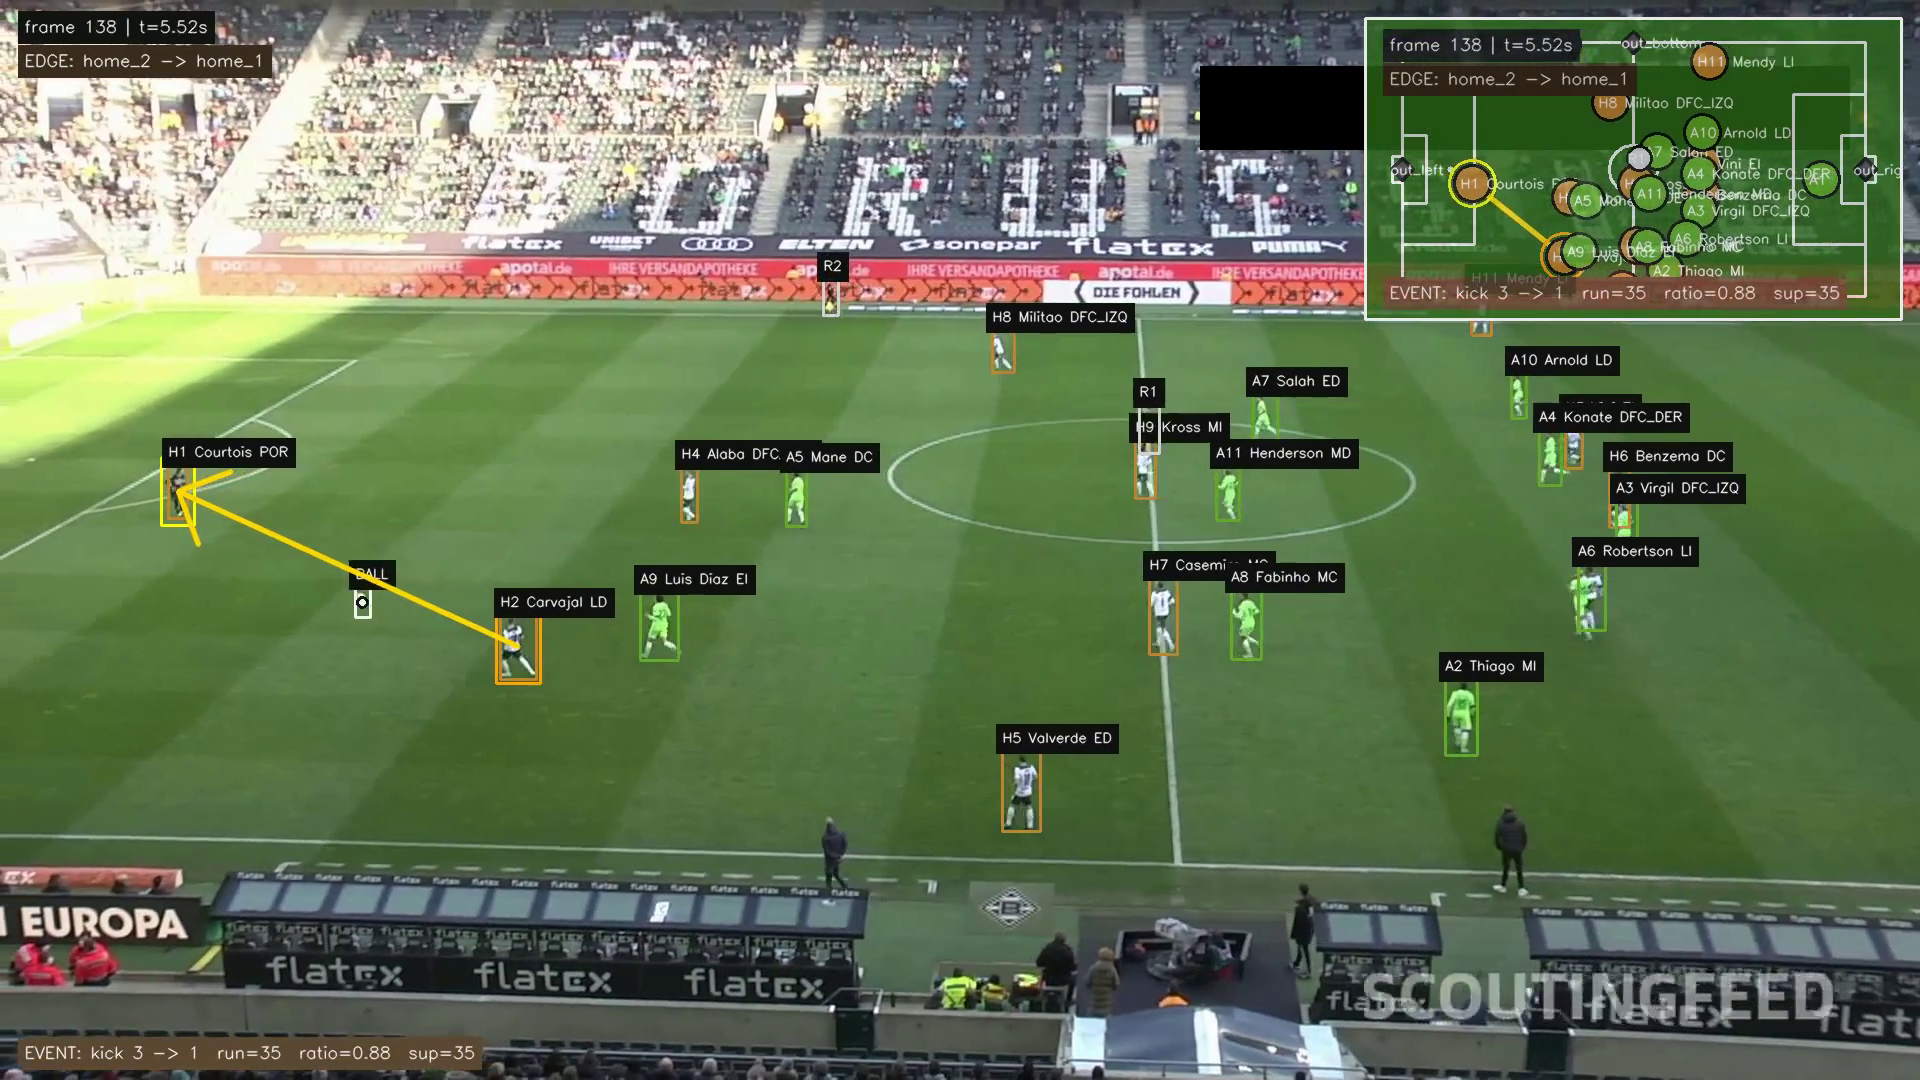
\includegraphics[width=0.95\textwidth]{Imagenes/Propias/tracking_pathcrf_frame.png}
    \caption[Resultado de la clasificación de acciones sobre una ventana temporal]{
    Resultado de la clasificación de acciones sobre una ventana temporal del partido. La salida de PathCRF se consolida mediante postprocesado temporal para obtener un único evento predominante por bloque de emisión, junto con su contexto temporal e identidad de los actores implicados.
    }
    \label{fig:resultado-clasificacion-acciones}
\end{figure}


\chapter{Narración}
\label{cap:narracion}

\section{Generación de comentarios}
\label{sec:generacion-comentarios}

Tras obtener las acciones del partido, el sistema ya dispone de la información necesaria para generar un comentario textual: la acción detectada, el instante en el que ocurre, el jugador asociado, su posición futbolística, su equipo y, cuando procede, información contextual adicional. El objetivo de esta fase no es construir una frase fija mediante reglas, sino utilizar un modelo generativo que permita obtener comentarios más naturales y con cierta variabilidad, manteniendo al mismo tiempo un control estricto sobre la información que puede aparecer en la respuesta.

\subsection{Variables de entrada del modelo}

La entrada al modelo se organiza como un evento estructurado en formato JSON. Esta decisión permite separar claramente dos partes del problema: por un lado, el pipeline anterior calcula la información objetiva del partido; por otro, el modelo de lenguaje transforma esa información en una frase natural de narrador.

Las variables principales utilizadas son las siguientes:

\begin{itemize}
    \item \texttt{action}: acción que se quiere comentar. Puede tomar valores como \texttt{control}, \texttt{pase}, \texttt{robo}, \texttt{tiro}, \texttt{corner}, \texttt{fuera de banda}, \texttt{saque de puerta}, \texttt{gol}, \texttt{intro} o \texttt{contexto}.

    \item \texttt{event\_time\_s}: segundo del vídeo en el que ocurre el evento.

    \item \texttt{player\_name}: nombre del jugador asociado a la acción.

    \item \texttt{player\_position}: posición futbolística del jugador, por ejemplo \texttt{MC}, \texttt{LI}, \texttt{ED} o \texttt{DC}.

    \item \texttt{team\_name}: equipo del jugador que realiza la acción.

    \item \texttt{opponent\_team\_name}: equipo rival. Se utiliza especialmente en goles e introducciones del partido.

    \item \texttt{team\_in\_favor}: equipo beneficiado en acciones como córner, saque de banda o saque de puerta.

    \item \texttt{action\_target}: destinatario u objetivo de la acción cuando existe esta información.

    \item \texttt{field\_zone}: zona del campo donde ocurre la acción, normalmente \texttt{zona de iniciación}, \texttt{zona de creación} o \texttt{zona de finalización}.

    \item \texttt{play\_context}: información contextual adicional. En comentarios de contexto puede incluir, por ejemplo, referencias tácticas a la defensa, al centro del campo o al ataque de un equipo.

    \item \texttt{match\_score}: contexto simulado de clasificación o situación del partido. Se utiliza para aportar información contextual, no para representar necesariamente el resultado real.

    \item \texttt{intensity}: marca ciertos eventos como interrupciones cuando aparece una acción peligrosa, como un tiro o un gol, durante un comentario de contexto.

    \item \texttt{action\_index}: índice secuencial de la acción dentro de la lista de eventos generada. Sirve principalmente para trazabilidad y depuración.
\end{itemize}

Estas variables permiten que el modelo disponga de información suficiente para generar comentarios coherentes sin inventar datos externos. Esta restricción es importante, ya que en una retransmisión automática resulta preferible generar un comentario sencillo pero correcto antes que una frase más vistosa con información no observada por el sistema.

\subsection{Diseño del prompt}

La generación del comentario se basa en dos prompts diferenciados: el \textit{system prompt} y el \textit{user prompt}. El primero define el rol general del modelo, mientras que el segundo contiene las instrucciones concretas para el evento actual.

El \textit{system prompt} establece el comportamiento global del modelo. Dependiendo del tipo de evento, el sistema cambia ligeramente el rol solicitado. Para una introducción, se le indica que actúe como un narrador de televisión abriendo la retransmisión antes de que comience el partido. Para un comentario de contexto, se le pide que actúe como comentarista de apoyo y que no narre una acción técnica concreta. En el caso de un gol, se permite un tono más expresivo, pero se imponen restricciones para evitar exageraciones o invenciones. Para el resto de acciones, se solicita una frase corta, natural y directa.

El \textit{user prompt}, en cambio, se construye de forma específica para cada evento. En él se incluyen reglas concretas como mencionar o no el minuto, utilizar literalmente la acción indicada, no inventar receptores en un pase, no añadir consecuencias posteriores a un gol o no repetir una frase reciente. Además, se adjunta el evento completo en formato JSON para que el modelo tenga acceso explícito a los datos disponibles.

Esta separación resulta útil porque permite mantener una personalidad general constante, pero ajustar las instrucciones según la naturaleza de cada evento. Por ejemplo, un comentario de introducción no debe mencionar acciones que todavía no han ocurrido, mientras que un gol debe mencionar claramente al autor, el equipo que marca y el equipo que encaja.

También se incorpora un mecanismo para reducir la repetición. Cuando el sistema dispone de un comentario reciente para una acción parecida, se añade al prompt una instrucción indicando que no debe repetirse la misma frase, ni el mismo verbo principal, ni la misma estructura. De esta forma se intenta mantener variabilidad sin perder fidelidad a los datos del evento.

\subsection{Selección del modelo de lenguaje}

Para generar los comentarios se probaron distintos modelos ligeros mediante Ollama. La prioridad era encontrar un equilibrio entre calidad lingüística, seguimiento de instrucciones y coste de inferencia. Dado que el comentario debe generarse a partir de eventos cortos y muy estructurados, no era necesario utilizar un modelo de gran tamaño, sino uno capaz de respetar bien el prompt y producir frases naturales en español.

\begin{table}[H]
    \centering
    \scriptsize
    \begin{tabular}{c|c}
        \textbf{Modelo} & \textbf{Tamaño} \\
        \hline\hline
        \texttt{gemma4:e2b} & 7.2 GB \\
        \texttt{qwen2:1.5b} & 934 MB \\
        \texttt{deepseek-r1:1.5b} & 1.1 GB \\
        \texttt{qwen3:1.7b} & 1.4 GB \\
        \texttt{lfm2.5-thinking:1.2b} & 731 MB \\
        \texttt{falcon3:1b} & 1.8 GB \\
        \texttt{granite4:1b} & 3.3 GB \\
        \texttt{gemma3:1b} & 815 MB \\
        \texttt{qwen3.5:2b} & 2.7 GB \\
        \texttt{qwen3:0.6b} & 522 MB \\
        \texttt{llama3.2:1b} & 1.3 GB \\
        \texttt{qwen3.5:0.8b} & 1.0 GB \\
        \texttt{tinyllama:1.1b} & 637 MB \\
        \texttt{qwen3.5:4b} & 3.4 GB \\
        \hline
    \end{tabular}
    \caption{Modelos probados para la generación de comentarios con Ollama.}
    \label{tab:modelos_llm_probados}
\end{table}


A partir de estas pruebas se observó que los modelos más pequeños de Qwen ofrecían una latencia favorable, pero la calidad de los comentarios no era suficiente para el tono buscado. En cambio, las variantes de mayor tamaño de Qwen mejoraban claramente la calidad lingüística, aunque su coste de inferencia aumentaba y dejaban de ser tan convenientes para una generación ágil dentro del sistema.

También se probó \texttt{lfm2.5-thinking:1.2b}, que generaba respuestas de buena calidad, pero presentaba una latencia demasiado alta para el objetivo del proyecto. Finalmente, el modelo que ofreció el mejor equilibrio observado entre naturalidad, seguimiento de instrucciones y tiempo de respuesta fue \texttt{gemma4:e2b}, por lo que se seleccionó como modelo principal para la generación de comentarios.

El principal inconveniente de utilizar directamente este modelo era su tamaño. Para reducir el consumo de recursos se optó por una versión cuantizada en formato \texttt{GGUF}, concretamente \texttt{gemma-4-E2B-it-Q4\_K\_S.gguf}. La cuantización consiste en representar los pesos del modelo con menor precisión numérica, reduciendo así el tamaño del modelo y el coste de inferencia. En este caso, \texttt{Q4} indica una cuantización principal a 4 bits, \texttt{K} hace referencia a una familia moderna de cuantizaciones por bloques, y \texttt{S} indica una variante más compacta.

Esta versión cuantizada ocupa aproximadamente 2.9 GB en disco, frente al tamaño mayor de la versión gestionada inicialmente mediante Ollama. Para ejecutarla se utilizó \texttt{llama.cpp}, una herramienta que permite desplegar modelos en formato \texttt{GGUF} de forma eficiente y exponerlos mediante una interfaz compatible con peticiones de chat. En la configuración del proyecto se utiliza un contexto de 512 tokens, suficiente para prompts cortos basados en eventos estructurados, y se desactiva el razonamiento explícito para evitar que el modelo genere explicaciones intermedias.

\subsection{Control de la salida generada}

Una vez recibido el comentario del modelo, el sistema aplica una limpieza básica de texto. Se eliminan espacios innecesarios, se normaliza la salida y se fuerza que el resultado final sea únicamente el comentario, sin explicaciones adicionales. Esto es importante porque algunos modelos tienden a responder con prefijos como ``Comentario:'' o a incluir aclaraciones que no forman parte de la frase final.

Además, el sistema evita comentar dos veces seguidas exactamente el mismo evento. Para ello se guarda una identidad simplificada del último evento generado, compuesta por la acción, el jugador y el equipo asociado. Si el siguiente evento coincide con esa misma identidad, se puede descartar para reducir duplicados.

En conjunto, esta fase transforma los eventos estructurados producidos por el pipeline en comentarios textuales naturales. La clave no está únicamente en elegir un modelo generativo, sino en controlar cuidadosamente qué información recibe, qué instrucciones debe seguir y qué restricciones impiden que invente contexto no observado por el sistema.

\subsection{Resultados de generación con eventos JSON}

Para comprobar el comportamiento del generador se levantó el modelo \texttt{gemma-4-E2B-it-Q4\_K\_S.gguf} mediante \texttt{llama.cpp}, utilizando el alias \texttt{gemma4-q4ks-text}. Las pruebas se realizaron con el servidor ya cargado en memoria.

Aunque la clase interna del evento define un conjunto amplio de campos posibles, el JSON que se introduce finalmente en el prompt no incluye siempre todas las claves: se eliminan los campos vacíos y se añade el campo \texttt{should\_mention\_minute}, que indica si el modelo debe mencionar explícitamente el minuto de partido.

\begin{table}[H]
    \centering
    \scriptsize
    \begin{tabular}{c|c|c|c}
        \textbf{Caso} & \textbf{Origen del evento} & \textbf{Tiempo total} & \textbf{Tiempo interno del modelo} \\
        \hline\hline
        Intro & Evento inicial con equipos & 0.311 s & 0.282 s \\
        Contexto & Evento construido desde alineación & 0.251 s & 0.238 s \\
        Pase & Evento real generado por PathCRF & 0.107 s & 0.094 s \\
        Tiro & Evento compatible con salida PathCRF & 0.101 s & 0.091 s \\
        Tiro con interrupción & Evento urgente con interrupción & 0.120 s & 0.113 s \\
        \hline
    \end{tabular}
    \caption{Tiempos de generación de comentarios con Gemma cuantizado ejecutado mediante \texttt{llama.cpp}.}
    \label{tab:tiempos_generacion_gemma}
\end{table}

\subsubsection*{Prueba 1: introducción}

\begin{verbatim}
{
  "action": "intro",
  "event_time_s": 0.0,
  "team_name": "Real Madrid",
  "opponent_team_name": "Wolfsburgo",
  "should_mention_minute": false
}
\end{verbatim}

Comentario generado:

\begin{quote}
¡Bienvenidos a todos! Ya está todo listo para este encuentro entre el Real Madrid y Wolfsburgo. ¡Que empiece la acción!
\end{quote}

\subsubsection*{Prueba 2: comentario de contexto}

\begin{verbatim}
{
  "action": "contexto",
  "event_time_s": 0.0,
  "team_name": "Real Madrid",
  "opponent_team_name": "Wolfsburgo",
  "field_zone": "zona de iniciacion",
  "play_context": "defensa de Real Madrid: centrales pepe y ramos",
  "match_score": "Real Madrid llega 3 en la tabla con 53 puntos; Wolfsburgo aparece 6 con 46 puntos",
  "action_index": 1,
  "should_mention_minute": false
}
\end{verbatim}

Comentario generado:

\begin{quote}
Con la defensa de Pepe y Ramos en el campo, el Real Madrid mantiene una ventaja en la clasificación, lo que les da tranquilidad en esta fase de salida de balón.
\end{quote}

\subsubsection*{Prueba 3: pase}

\begin{verbatim}
{
  "action": "pase",
  "event_time_s": 0.0,
  "player_name": "Carvajal",
  "player_position": "LD",
  "team_name": "Real Madrid",
  "action_target": "vini",
  "action_index": 1,
  "should_mention_minute": false
}
\end{verbatim}

Comentario generado:

\begin{quote}
Carvajal realiza un pase a Vini.
\end{quote}

\subsubsection*{Prueba 4: tiro}

\begin{verbatim}
{
  "action": "tiro",
  "event_time_s": 24.2,
  "player_name": "cristiano",
  "player_position": "DC",
  "team_name": "Real Madrid",
  "field_zone": "zona de finalizacion",
  "action_index": 28,
  "should_mention_minute": false
}
\end{verbatim}

Comentario generado:

\begin{quote}
Cristiano tira con potencia en la zona de finalización.
\end{quote}

\subsubsection*{Prueba 5: tiro con interrupción}

\begin{verbatim}
{
  "action": "tiro",
  "event_time_s": 24.6,
  "player_name": "cristiano",
  "player_position": "DC",
  "team_name": "Real Madrid",
  "field_zone": "zona de finalizacion",
  "play_context": "hay que cortar un comentario de contexto porque aparece una accion peligrosa",
  "intensity": "interrupcion",
  "action_index": 29,
  "should_mention_minute": false
}
\end{verbatim}

Comentario generado:

\begin{quote}
Perdon, te corto, Cristiano tira en la zona de finalización.
\end{quote}

Estos resultados muestran que el modelo responde de forma distinta según el tipo de evento. En acciones simples, como un pase o un tiro, genera frases breves y directas. En el evento de contexto utiliza la información táctica disponible y el contexto simulado de clasificación. Por último, cuando aparece \texttt{intensity = interrupcion}, el comentario adopta una forma de interrupción breve antes de narrar la acción peligrosa.


\section{Sistema de síntesis de audio}
\label{sec:sintesis-voz-pipeline}

Esta sección describe el sistema de síntesis de voz del proyecto a partir del momento en que el comentario textual ya ha sido generado, se realizarán pruebas con distintos enfoques y distintos modelos de sintesis de voz

\subsection{Objetivo}

El objetivo es transformar el texto en una locución natural, con una voz adecuada para una retransmisión deportiva y con una latencia lo suficientemente baja como para que el resultado pueda utilizarse en una demostración interactiva

Durante el desarrollo se evaluaron varias alternativas de síntesis. Primero se trabajó con XTTS clonando muestras de voz propias, ya que era una solución local y rápida. Después se exploró Qwen TTS, porque su módulo de VoiceDesign generaba voces de locutor con una calidad subjetiva superior. Sin embargo, el modelo de generación de audio de Qwen resultó demasiado lento para utilizarlo directamente. A partir de esa observación se adoptó un enfoque mixto: utilizar Qwen VoiceDesign para crear una voz de referencia y después sintetizar los comentarios con XTTS. Finalmente, se incorporó ElevenLabs como última alternativa probada, orientada a demos con voces comerciales creadas mediante Voice Design y consumidas a través de API.

\subsection{Entrada del sistema de audio}

La entrada del sistema de audio es siempre un comentario completo en texto. La síntesis no comienza mientras se genera la frase palabra por palabra, sino cuando el comentario ya está cerrado y puede enviarse a un backend de voz.

A partir de ese texto, el sistema realiza tres operaciones principales:

\begin{enumerate}
    \item Selecciona el backend de síntesis configurado.
    \item Selecciona la voz del comentarista.
    \item Genera el audio correspondiente.
\end{enumerate}

Esta separación permite comparar diferentes motores de voz manteniendo constante la entrada textual. De este modo, el mismo comentario puede sintetizarse con XTTS, con Qwen, con una combinación Qwen VoiceDesign + XTTS o con ElevenLabs. Estas comparaciones, junto con los resutlados obtenidos, se describen a continuación.

\subsection{Primeras pruebas con XTTS y clonación de voz}

La primera solución utilizada fue XTTS. Se eligió porque permite síntesis local, no depende de servicios externos y ofrece una latencia baja una vez cargado el modelo. XTTS, cuya arquitectura se detalla en la \hyperref[sec:síntesis-voz]{Sección~\ref*{sec:síntesis-voz}} funciona mediante clonación de voz: recibe una muestra de referencia y genera nuevos audios intentando conservar una identidad vocal similar.

En las primeras pruebas se utilizó XTTS clonando muestras propias. Esta vía era funcional y rápida, pero el resultado sonoro no alcanzaba todavía la expresividad esperada para una narración deportiva. La voz era suficiente para validar el pipeline, pero no tenía una sensación clara de locutor profesional.

Por este motivo se comenzó a buscar una referencia vocal mejor. La pregunta que guió la siguiente fase fue si se podía obtener una voz más radiofónica sin renunciar a la baja latencia de XTTS.

\subsection{Qwen TTS}

La siguiente línea de trabajo fue Qwen TTS. Esta prueba se planteó porque Qwen ofrecía un módulo específico de diseño de voz capaz de generar una referencia vocal más convincente para un narrador deportivo. La idea inicial no era únicamente sintetizar audio, sino comprobar si se podía obtener una voz con más presencia radiofónica que las primeras referencias utilizadas con XTTS.

La ruta evaluada estaba compuesta por dos partes:

\begin{itemize}
    \item \texttt{Qwen/Qwen3-TTS-12Hz-1.7B-VoiceDesign}, utilizado para diseñar la voz de locutor.
    \item \texttt{Qwen/Qwen3-TTS-12Hz-0.6B-Base} o \texttt{Qwen/Qwen3-TTS-12Hz-1.7B-Base}, utilizados para reutilizar esa identidad vocal y sintetizar nuevos comentarios.
\end{itemize}

La primera integración funcional confirmó que la calidad potencial de la voz era buena, pero también mostró que la latencia era demasiado elevada para utilizar Qwen como sintetizador principal. Aunque el flujo funcionaba, el tiempo de síntesis hacía inviable esta ruta para una demo interactiva. A partir de ese punto se realizaron varias pruebas para intentar reducir la latencia.

\subsection{Optimización de Qwen}

Tras comprobar que Qwen ofrecía una voz más convincente que las primeras referencias usadas con XTTS, se realizaron varias pruebas para reducir su latencia. La arquitectura evaluada estaba formada por dos modelos: \texttt{Qwen/Qwen3-TTS-12Hz-1.7B-VoiceDesign}, encargado de diseñar la voz de locutor, y un modelo Base encargado de reutilizar esa identidad vocal para sintetizar nuevos comentarios.

Se compararon dos modelos Base, \texttt{Qwen/Qwen3-TTS-12Hz-1.7B-Base} y \texttt{Qwen/Qwen3-TTS-12Hz-0.6B-Base}, con y sin FlashAttention. Como se observa en la \hyperref[tab:parametros-FlashAttention]{Tabla~\ref*{tab:parametros-FlashAttention}}, todas las filas pertenecen al mismo benchmark controlado, por lo que los valores sí son comparables entre sí.

\begin{table}[ht]
\centering
\begin{tabular}{lcccc}
\toprule
Configuración & Carga voz & Carga modelo & Primera petición & Media caliente \\
\midrule
1.7B sin FlashAttention & 3.442 s & 4.565 s & 15.998 s & 18.370 s \\
1.7B con FlashAttention & 3.368 s & 4.499 s & 15.860 s & 20.589 s \\
0.6B sin FlashAttention & 3.447 s & 4.366 s & 13.235 s & 16.938 s \\
0.6B con FlashAttention & 3.372 s & 4.383 s & 14.274 s & 19.194 s \\
\bottomrule
\end{tabular}
\caption{Comparativa controlada de Qwen Base reutilizando una voz diseñada previamente con Qwen VoiceDesign.}
\label{tab:parametros-FlashAttention}
\end{table}

La configuración más razonable fue \texttt{Qwen/Qwen3-TTS-12Hz-0.6B-Base} sin FlashAttention. El modelo 0.6B reducía el coste general frente al 1.7B y, en esta máquina, FlashAttention no produjo una mejora real. De hecho, las variantes con FlashAttention fueron peores en la media de peticiones posteriores.

Es importante aclarar que la columna ``Primera petición'' no representa la primera ejecución absoluta del sistema, sino la primera petición dentro de ese benchmark una vez cargados la voz y el modelo. La columna ``Media caliente'' mide peticiones posteriores con el proceso vivo, pero no siempre tiene por qué ser menor, ya que las frases evaluadas no tienen exactamente la misma longitud ni complejidad. Por tanto, esta tabla sirve para comparar configuraciones entre sí, no para afirmar que toda primera llamada sea necesariamente más lenta que cualquier llamada posterior.

Aun así, en un sistema real sí es habitual que la primera ejecución completa tarde más que las siguientes. La primera llamada puede incluir inicialización de CUDA, reserva de memoria, carga de pesos, preparación de cachés internas, inicialización del vocoder y calentamiento de kernels.

Incluso después de estas optimizaciones, Qwen seguía quedando lejos de XTTS. La mejora de calidad vocal era clara, pero la latencia seguía siendo demasiado alta para utilizar Qwen como sintetizador principal en la demo.

\subsection{Evaluación de qwen3-tts.cpp}

Como la ruta de Qwen con Python seguía siendo lenta, se probó una implementación experimental basada en \texttt{qwen3-tts.cpp}. Esta vía utilizaba modelos cuantizados en formato GGUF, reutilización de \textit{speaker embedding} y un runtime persistente.

La primera prueba funcionó, pero se ejecutaba principalmente en CPU. Como se muestra en la \hyperref[tab:qwen-cpp-cpu]{Tabla~\ref*{tab:qwen-cpp-cpu}}, esta ruta todavía no aprovechaba la GPU y la síntesis seguía siendo demasiado lenta para una demo interactiva.

\begin{table}[ht]
\centering
\begin{tabular}{lccc}
\toprule
Ruta & LLM / preparación & Síntesis & Total \\
\midrule
qwen3-tts.cpp en CPU & 4.672 s & 24.461 s & 29.133 s \\
\bottomrule
\end{tabular}
\caption{Prueba inicial de qwen3-tts.cpp ejecutándose principalmente en CPU.}
\label{tab:qwen-cpp-cpu}
\end{table}

Los resultados en CPU quedaban por encima de los tiempos esperados para una demo interactiva, por lo que el siguiente paso fue reconstruir la librería con soporte CUDA real.

Después de activar CUDA, tanto el transformer TTS como el decodificador de audio pasaron a ejecutarse en GPU. Como puede verse en la \hyperref[tab:qwen-cpp-cuda]{Tabla~\ref*{tab:qwen-cpp-cuda}}, en este caso sí hubo una mejora clara frente a la ruta C++ en CPU.

\begin{table}[ht]
\centering
\begin{tabular}{lccc}
\toprule
Ruta & LLM / preparación & Síntesis & Total \\
\midrule
qwen3-tts.cpp con CUDA & 4.378 s & 12.582 s & 16.959 s \\
\bottomrule
\end{tabular}
\caption{Mejora obtenida al activar CUDA en qwen3-tts.cpp.}
\label{tab:qwen-cpp-cuda}
\end{table}

También se ajustó el número de hilos del runtime. Esta prueba medía el tiempo medio de síntesis de \texttt{qwen3-tts.cpp} con CUDA, no el pipeline completo con LLM ni preparación. Por eso estos valores, recogidos en la \hyperref[tab:qwen-cpp-hilos]{Tabla~\ref*{tab:qwen-cpp-hilos}}, no son directamente comparables con los totales de las tablas anteriores.

\begin{table}[ht]
\centering
\begin{tabular}{lc}
\toprule
Hilos & Tiempo medio de síntesis \\
\midrule
4 & 9.744 s \\
6 & 9.333 s \\
8 & 10.709 s \\
10 & 9.726 s \\
12 & 10.573 s \\
\bottomrule
\end{tabular}
\caption{Ajuste de hilos en qwen3-tts.cpp con CUDA. La métrica corresponde a síntesis del runtime, no al pipeline completo.}
\label{tab:qwen-cpp-hilos}
\end{table}

La configuración más estable fue de 6 hilos. Aun así, la mejora no cambiaba la conclusión principal: \texttt{qwen3-tts.cpp} con CUDA era bastante más rápido que su versión en CPU, pero seguía siendo más lento que XTTS en caliente.

Para cerrar la comparación se evaluaron XTTS y \texttt{qwen3-tts.cpp} sobre el mismo comentario corto. Como se resume en la \hyperref[tab:xtts-qwen-cpp]{Tabla~\ref*{tab:xtts-qwen-cpp}}, esta medición sí es una comparación directa entre sistemas para el caso de uso del proyecto.

\begin{table}[ht]
\centering
\begin{tabular}{lccc}
\toprule
Sistema & Síntesis caliente & Duración del audio & Fin de escucha \\
\midrule
XTTS con referencia local & 1.581 s & 3.243 s & 4.824 s \\
qwen3-tts.cpp con CUDA & 14.188 s & 3.657 s & 17.844 s \\
\bottomrule
\end{tabular}
\caption{Comparativa caliente entre XTTS y qwen3-tts.cpp con CUDA sobre el mismo comentario.}
\label{tab:xtts-qwen-cpp}
\end{table}

Como comparación auditiva directa entre ambos sintetizadores, se incluyen las dos muestras generadas sobre el mismo comentario:

\begin{center}
\audiolink{Escuchar XTTS}{https://raw.githubusercontent.com/hectorgarciaa/narrador-futbol/final/audios/compare_xtts.wav}
\qquad
\audiolink{Escuchar Qwen C++}{https://raw.githubusercontent.com/hectorgarciaa/narrador-futbol/final/audios/compare_qwen_cpp.wav}
\end{center}

La conclusión final fue que Qwen no resultaba adecuado como sintetizador principal para el modo en directo. Su calidad vocal era prometedora, pero la latencia seguía siendo demasiado alta. Sin embargo, Qwen sí aportó valor como herramienta de diseño de voz: la solución más práctica fue utilizar \texttt{Qwen VoiceDesign} para generar una referencia vocal de locutor y después sintetizar los comentarios finales con XTTS. De esta forma se aprovechaba el mejor timbre de Qwen sin renunciar a la baja latencia de XTTS.

\subsection{Enfoque mixto: Qwen VoiceDesign + XTTS}

El resultado más importante de las pruebas con Qwen fue comprobar que el diseño de voz era útil, aunque el sintetizador completo no fuese lo bastante rápido. La voz creada por \texttt{Qwen/Qwen3-TTS-12Hz-1.7B-VoiceDesign} sonaba más adecuada para una narración deportiva que las primeras referencias propias usadas con XTTS.

Por ello se adoptó un enfoque mixto:

\begin{enumerate}
    \item Usar Qwen VoiceDesign para generar una voz de locutor deportivo.
    \item Guardar esa voz como muestra de referencia.
    \item Usar XTTS para sintetizar los comentarios finales clonando esa referencia.
\end{enumerate}

La idea no era sustituir XTTS por Qwen, sino aprovechar la mejor parte de cada sistema: Qwen para diseñar la identidad vocal y XTTS para generar los audios con baja latencia. Como se observa en la \hyperref[tab:qwen-voicedesign-xtts]{Tabla~\ref*{tab:qwen-voicedesign-xtts}}, la penalización temporal de este enfoque fue muy reducida.

\begin{table}[ht]
\centering
\begin{tabular}{lc}
\toprule
Caso & Tiempo de síntesis \\
\midrule
XTTS con voz diseñada por Qwen, primera pasada & 3.790 s \\
XTTS con voz diseñada por Qwen, ejecución caliente 1 & 1.276 s \\
XTTS con voz diseñada por Qwen, ejecución caliente 2 & 0.939 s \\
XTTS con referencia habitual & 0.880 s \\
\bottomrule
\end{tabular}
\caption{Uso de una voz diseñada con Qwen VoiceDesign como referencia para XTTS.}
\label{tab:qwen-voicedesign-xtts}
\end{table}

La penalización de latencia fue mínima, mientras que la mejora subjetiva del timbre fue apreciable. Esta fue la solución local más equilibrada: no dependía de una API externa, mantenía tiempos cercanos a XTTS y producía una voz más convincente.

Para apreciar la diferencia entre la voz diseñada por Qwen y el resultado final sintetizado con XTTS, se incluyen las siguientes muestras:

\begin{center}
\audiolink{Escuchar voz diseñada por Qwen}{https://raw.githubusercontent.com/hectorgarciaa/narrador-futbol/final/audios/qwen_voice_design_reference.wav}
\qquad
\audiolink{Escuchar Qwen VoiceDesign + XTTS}{https://raw.githubusercontent.com/hectorgarciaa/narrador-futbol/final/audios/xtts_from_qwen_voice_design.wav}
\end{center}

\subsection{Pruebas por tipo de comentario con el enfoque mixto}

Una vez validado el enfoque Qwen VoiceDesign + XTTS, se generó una tanda de comentarios con varios tipos de acción, cuyos tiempos de síntesis se reflejan en la \hyperref[tab:comparacion_tiempo_acciones]{Tabla~\ref*{tab:comparacion_tiempo_acciones}}. El objetivo era comprobar cómo afectaba la longitud del texto a la síntesis y al tiempo total de escucha.

\begin{table}[ht]
\centering
\begin{tabular}{lcccc}
\toprule
Acción & Preparación & Síntesis & Duración audio & Fin de escucha \\
\midrule
Pase largo & 0.397 s & 1.043 s & 3.574 s & 5.014 s \\
Tiro & 0.385 s & 0.713 s & 2.497 s & 3.595 s \\
Control & 0.359 s & 1.624 s & 5.430 s & 7.413 s \\
Corner & 0.354 s & 0.967 s & 3.339 s & 4.660 s \\
Robo & 0.374 s & 0.894 s & 3.105 s & 4.373 s \\
\bottomrule
\end{tabular}
\caption{Medición por tipo de acción usando XTTS con voz diseñada previamente mediante Qwen VoiceDesign.}
\label{tab:comparacion_tiempo_acciones}
\end{table}

A continuación se incluyen las muestras generadas para cada tipo de acción evaluado:

\begin{center}
\begin{tabular}{ll}
Gol & \audiolink{Escuchar gol}{https://raw.githubusercontent.com/hectorgarciaa/narrador-futbol/final/audios/01_gol.wav} \\[0.35cm]
Pase largo & \audiolink{Escuchar pase largo}{https://raw.githubusercontent.com/hectorgarciaa/narrador-futbol/final/audios/02_pase_largo.wav} \\[0.35cm]
Tiro & \audiolink{Escuchar tiro}{https://raw.githubusercontent.com/hectorgarciaa/narrador-futbol/final/audios/03_tiro.wav} \\[0.35cm]
Control & \audiolink{Escuchar control}{https://raw.githubusercontent.com/hectorgarciaa/narrador-futbol/final/audios/04_control.wav} \\[0.35cm]
Corner & \audiolink{Escuchar corner}{https://raw.githubusercontent.com/hectorgarciaa/narrador-futbol/final/audios/05_corner.wav} \\[0.35cm]
Robo & \audiolink{Escuchar robo}{https://raw.githubusercontent.com/hectorgarciaa/narrador-futbol/final/audios/06_robo.wav} \\
\end{tabular}
\end{center}

Estas pruebas muestran que la duración del comentario es uno de los factores dominantes. Las acciones breves, como tiros, robos o corners, son mucho más adecuadas para baja latencia. Los goles, al ser comentarios más expresivos y largos, aumentan de forma natural el tiempo hasta finalizar la escucha.

\subsection{Alternancia entre dos comentaristas}

Una vez resuelta la síntesis, se mantuvo la idea de utilizar dos voces: una masculina y una femenina. El objetivo es que la narración se parezca más a una retransmisión real, con un comentarista principal y una voz de apoyo.

La alternancia no sigue un patrón fijo, sino una selección aleatoria controlada. El sistema evita que una misma voz intervenga demasiadas veces seguidas. Esta lógica es independiente del backend de síntesis: puede utilizarse con XTTS y referencias locales, con XTTS usando voces diseñadas por Qwen, o con voces de ElevenLabs.

\subsection{ElevenLabs como última alternativa evaluada}

Después de las pruebas locales con XTTS, Qwen y el enfoque mixto, se evaluó ElevenLabs. Esta fue la última alternativa probada. La motivación fue comprobar si una voz comercial creada mediante Voice Design podía ofrecer una calidad superior para una demostración final.

A diferencia de XTTS y Qwen, ElevenLabs no genera el audio localmente. El sistema envía el texto completo del comentario a la API y recibe la locución generada. Esta integración mantiene la arquitectura existente, pero cambia el origen del audio: en lugar de sintetizarse en local, se obtiene desde un servicio externo.

ElevenLabs permite además streaming de audio. En este proyecto, esto significa que el texto completo se envía al servicio y la API empieza a devolver fragmentos de audio mientras termina la síntesis. No se trata de ir pronunciando palabras a medida que se genera el texto, porque el comentario textual ya llega completo.

\subsection{Evaluación de modelos de ElevenLabs}

Para comparar ElevenLabs se utilizó un comentario breve de apertura. Se midió el tiempo hasta recibir el primer fragmento de audio, el tiempo hasta completar el stream, el instante estimado de la primera palabra y el instante estimado de la última palabra, como se puede observar en la Tabla~\ref{tab:comparacion_11labs}.

\begin{table}[ht]
\centering
\small
\setlength{\tabcolsep}{4pt}
\begin{tabular}{lcccc}
\toprule
Modelo & \makecell{Primer\\fragmento} & \makecell{Stream\\completo} & \makecell{Primera\\palabra} & \makecell{Última\\palabra} \\
\midrule
\texttt{eleven\_flash\_v2\_5}     & 0.867 s & 0.936 s & 0.983 s & 5.349 s \\
\texttt{eleven\_multilingual\_v2} & 0.998 s & 1.022 s & 1.056 s & 5.398 s \\
\texttt{eleven\_v3}               & 1.866 s & 2.735 s & 1.946 s & 6.806 s \\
\bottomrule
\end{tabular}
\caption{Latencias medidas con distintos modelos de ElevenLabs.}
\label{tab:comparacion_11labs}
\end{table}

Para comparar también la calidad percibida de cada modelo, se incluyen las tres muestras generadas con el mismo comentario de introducción:

\begin{center}
\begin{tabular}{ll}
Flash v2.5 & \audiolink{Escuchar Flash v2.5}{https://raw.githubusercontent.com/hectorgarciaa/narrador-futbol/final/audios/intro_flash_v2_5.wav} \\[0.4cm]
Multilingual v2 & \audiolink{Escuchar Multilingual v2}{https://raw.githubusercontent.com/hectorgarciaa/narrador-futbol/final/audios/intro_multilingual_v2.wav} \\[0.4cm]
Eleven v3 & \audiolink{Escuchar Eleven v3}{https://raw.githubusercontent.com/hectorgarciaa/narrador-futbol/final/audios/intro_v3.wav} \\
\end{tabular}
\end{center}

El modelo \texttt{eleven\_flash\_v2\_5} fue el más rápido, pero con menor calidad percibida. \texttt{eleven\_v3} ofreció una voz más expresiva, aunque con una latencia claramente superior. Finalmente se seleccionó \texttt{eleven\_multilingual\_v2}, porque ofrecía el mejor equilibrio entre calidad, coste y tiempo de respuesta.

\subsection{Decisión final}

La evaluación dejó una conclusión clara: Qwen generaba una voz de referencia muy interesante, pero no era suficientemente rápido como sintetizador completo. XTTS era mucho más rápido, pero las primeras referencias propias no tenían la calidad vocal deseada. Esto queda reflejado en la Tabla~\ref{tab:soluciones-sintesis}. El enfoque mixto Qwen VoiceDesign + XTTS resolvió ese conflicto: Qwen se usa para diseñar la voz y XTTS para sintetizar los comentarios.

\begin{table}[ht]
\centering
\begin{tabular}{lll}
\toprule
Sistema & Ventaja principal & Uso recomendado \\
\midrule
XTTS con referencia propia & Baja latencia local & Validación inicial y baseline \\
Qwen completo & Voz prometedora, latencia alta & Investigación y comparación \\
Qwen VoiceDesign + XTTS & Buen timbre con baja latencia & Solución local más equilibrada \\
ElevenLabs Multilingual v2 & Mayor naturalidad comercial & Demo final de alta calidad \\
\bottomrule
\end{tabular}
\caption{Resumen de las soluciones de síntesis evaluadas.}
\label{tab:soluciones-sintesis}
\end{table}

ElevenLabs se mantiene como alternativa externa para demos donde la calidad de voz sea prioritaria. XTTS sigue siendo la base local por su baja latencia, y Qwen queda como herramienta útil de diseño de voz y como línea experimental para futuras optimizaciones.

\chapter{Conclusiones y Trabajo Futuro}
\label{cap:conclusiones}

\section{Conclusiones globales}

El objetivo de este trabajo era construir un sistema capaz de transformar un partido de fútbol en una narración automática, integrando visión por computador, seguimiento de jugadores, identificación de equipos, detección de acciones, generación de comentarios e incorporación de voz. El resultado final no alcanza todavía el comportamiento de una retransmisión profesional en tiempo real, pero sí demuestra que el pipeline completo es viable y que cada una de sus etapas produce una salida suficientemente coherente como para alimentar a la siguiente.

Una de las conclusiones principales del proyecto es que el problema no se resuelve con un único modelo, sino mediante la coordinación de muchos componentes especializados. La detección localiza jugadores, balón y árbitro; el tracking mantiene identidades a lo largo del tiempo; la asignación de equipos permite diferenciar a los jugadores por color; la alineación introducida en la interfaz ayuda a asociar posiciones y nombres; la detección de acciones transforma trayectorias en eventos narrables; el modelo de lenguaje convierte esos eventos en texto; y el sistema de síntesis de voz convierte finalmente ese texto en audio. La dificultad real aparece precisamente en la acumulación de pequeños errores entre módulos.

Aun así, el sistema construido permite recorrer todas las fases del proceso. Se ha conseguido pasar desde un vídeo de entrada hasta un vídeo procesado con comentarios generados automáticamente, alternando voces de comentaristas y permitiendo tanto una reproducción en directo simulada como un ensamblado posterior más alineado temporalmente. 

Los resultados también muestran que la latencia sigue siendo el principal obstáculo para una narración verdaderamente en tiempo real. La GPU utilizada durante el desarrollo, una NVIDIA RTX 3080, ha sido imprescindible para poder entrenar, ejecutar detección, probar modelos de voz y realizar experimentos de inferencia local. Sin embargo, para un proyecto tan ambicioso, en el que varias fases compiten por los mismos recursos de cómputo, se queda limitada. Una GPU más potente reduciría parte de la latencia local, especialmente en detección, tracking y síntesis basada en modelos locales, pero no eliminaría por completo los retrasos introducidos por servicios externos como ElevenLabs, donde existe una latencia de red y de generación que ronda aproximadamente el segundo incluso usando streaming.

En este sentido, una conclusión práctica es que una retransmisión automática completamente sincronizada puede requerir introducir un pequeño retardo controlado en la visualización del vídeo. En un escenario de emisión real, retrasar ligeramente la imagen permitiría disponer de margen para detectar la acción, generar el comentario y reproducirlo de forma más natural. Esta estrategia es habitual en sistemas donde prima la coherencia audiovisual frente a la inmediatez absoluta.

\section{Consideraciones sobre licencias y recursos externos}

Durante el desarrollo se han utilizado herramientas, modelos y conjuntos de datos de terceros. Aunque el proyecto se ha realizado con finalidad académica, no todos estos recursos tienen las mismas condiciones de uso. Algunos son abiertos y pueden utilizarse sin pago, otros son abiertos pero imponen obligaciones fuertes, y otros dependen de servicios comerciales o de licencias específicas.

En la parte de detección se ha utilizado YOLO mediante Ultralytics. Ultralytics ofrece sus modelos y herramientas bajo un esquema dual. La opción abierta es AGPL-3.0, una licencia que permite usar, modificar y distribuir el software sin pagar, pero exige que los proyectos derivados cumplan también las obligaciones de la AGPL. En la práctica, si se integra Ultralytics YOLO en una aplicación distribuida o en un servicio, habría que liberar el código correspondiente bajo una licencia compatible. Si se quisiera utilizar YOLO de Ultralytics en un producto cerrado, propietario o comercial sin abrir el código, sería necesario adquirir una licencia Enterprise de Ultralytics.

Para el tracking se ha utilizado \textit{supervision}, incluyendo la integración con ByteTrack. Esta librería está publicada bajo licencia MIT, que es una licencia abierta y permisiva. Permite uso académico, personal y comercial, modificación y redistribución, sin necesidad de pago, siempre que se mantengan los avisos de copyright y la licencia original.

El conjunto de vídeos de Kaggle \textit{DFL Bundesliga 460 MP4 Videos in 30Sec. + CSV} está publicado bajo licencia CC BY-SA 4.0. Se trata de una licencia abierta que permite usar, compartir y adaptar el material, incluso con fines comerciales, siempre que se cite adecuadamente la fuente. Además, al ser una licencia \textit{ShareAlike}, cualquier adaptación o material derivado que se redistribuya debe hacerse bajo la misma licencia o una compatible. Por tanto, no requiere pago, pero sí atribución y conservación de la misma filosofía de licencia en derivados redistribuidos.

Para el entrenamiento de detección también se ha utilizado el dataset \textit{FootBall Detection} disponible en Roboflow Universe, proporcionado por un usuario de Roboflow. Este dataset está publicado bajo licencia CC BY 4.0. Esta licencia es abierta y más permisiva que CC BY-SA: permite uso, copia, modificación, distribución y uso comercial sin necesidad de pago, siempre que se cite correctamente al autor, se enlace la licencia y se indiquen los cambios realizados si los hubiera. A diferencia de CC BY-SA, no obliga a publicar las adaptaciones bajo la misma licencia.

También se han utilizado datos sintéticos de SoccerSynth/Spiideo SoccerNet SynLoc. En este caso la licencia es más restrictiva: salvo que el dataset indique otra cosa, Spiideo lo ofrece bajo CC BY-NC-SA 4.0 con términos adicionales. Esto significa que puede utilizarse para investigación y experimentación no comercial, citando la fuente y manteniendo la misma licencia en derivados, pero no puede emplearse libremente en un producto comercial. Además, los términos de Spiideo prohíben redistribuir directamente el dataset a terceros, por lo que otros usuarios deberían obtenerlo desde la fuente oficial. Para un uso comercial habría que solicitar autorización o una licencia específica.

Para la detección de acciones se ha integrado PathCRF. El código de PathCRF está publicado bajo licencia MPL-2.0, una licencia abierta que permite uso, modificación y uso comercial sin pago. Sin embargo, no es tan permisiva como MIT: si se modifican archivos cubiertos por MPL-2.0 y se distribuyen, esos archivos modificados deben mantenerse bajo MPL-2.0. PathCRF se apoya originalmente en datos como Sportec Open DFL Dataset, publicado bajo CC BY 4.0. Este dataset permite uso y adaptación, también comercial, siempre que se cite correctamente la fuente.

En la generación de comentarios se ha utilizado Gemma 4, de Google. Gemma 4 está publicado bajo licencia Apache 2.0, una licencia abierta y permisiva. Permite uso académico y comercial, modificación y redistribución sin pago, siempre que se mantengan los avisos de copyright, licencia y atribución correspondientes. Al tratarse de un modelo generativo, además de la licencia conviene respetar las recomendaciones de uso responsable asociadas al modelo.

En la síntesis de voz se han evaluado varias alternativas. XTTS-v2, de Coqui, está publicado bajo la Coqui Public Model License. Esta licencia permite el uso no comercial del modelo y de sus salidas, pero no es una licencia abierta permisiva. Por tanto, XTTS-v2 resulta válido para investigación, pruebas y este proyecto académico, pero no debería utilizarse directamente en un producto comercial sin una licencia o autorización adecuada.

Qwen3-TTS, de Alibaba/Qwen, aparece publicado en Hugging Face bajo licencia Apache 2.0 para los modelos utilizados, incluyendo \texttt{Qwen/Qwen3-TTS-12Hz-1.7B-VoiceDesign} y los modelos \texttt{Base}. En este caso se trata de una licencia abierta y permisiva, por lo que permite uso académico, modificación y uso comercial sin pago, manteniendo los avisos de licencia correspondientes.

ElevenLabs es un caso diferente, ya que no se utiliza como un modelo descargado y ejecutado localmente, sino como un servicio propietario mediante API. No es una solución abierta ni gratuita en producción. Su uso depende de los términos de servicio de ElevenLabs, del sistema de créditos y del plan contratado. Para una demo puede utilizarse con una cuenta y cuota disponible, pero para un uso continuado o comercial habría que asumir el coste del servicio. Además, las voces creadas con Voice Design no se descargan como modelos locales independientes, sino que se consumen dentro de la plataforma de ElevenLabs.

En resumen, los componentes más permisivos del proyecto son \textit{supervision}/ByteTrack, el dataset de Roboflow bajo CC BY 4.0, Sportec Open DFL Dataset, Gemma 4 y Qwen3-TTS. El dataset de Kaggle bajo CC BY-SA 4.0 también es abierto, pero exige mantener la misma licencia en adaptaciones redistribuidas. PathCRF es abierto bajo MPL-2.0, aunque con obligaciones sobre archivos modificados. Ultralytics YOLO puede utilizarse sin pagar bajo AGPL-3.0 si el proyecto cumple sus requisitos de apertura, pero requiere licencia Enterprise para uso propietario cerrado. SoccerSynth/Spiideo está orientado a investigación no comercial y no permite redistribución directa del dataset. XTTS-v2 queda limitado a uso no comercial bajo CPML. ElevenLabs, finalmente, es un servicio propietario de pago por uso o suscripción.

\section{Limitaciones del sistema}

La principal limitación del proyecto es la latencia acumulada. Cada etapa introduce un pequeño coste temporal y, cuando se combinan detección, tracking, identificación, detección de acciones, generación textual y síntesis de audio, el retraso total puede ser perceptible. El sistema funciona mejor cuando puede procesar el vídeo con un pequeño margen o cuando se ensambla el audio en diferido.

Otra limitación importante es que el sistema trabaja con vídeos ya grabados. Aunque se ha simulado un modo en directo, todavía no se ha conectado una cámara real como fuente de entrada continua. Esto implicaría resolver nuevos problemas de captura, buffering, estabilidad de FPS, pérdida de frames, sincronización audiovisual y despliegue en campo.

También existen limitaciones en la detección de acciones. Actualmente se han considerado acciones suficientes para generar una narración básica, pero el fútbol contiene muchos eventos difíciles de reconocer únicamente a partir de trayectorias: faltas, ventajas, tarjetas, fueras de juego, disputas aéreas, cambios de orientación o acciones tácticas más complejas. Algunas de estas acciones requerirían incorporar pose del árbitro, pose de jugadores, contexto temporal más amplio o modelos entrenados específicamente con más datos anotados.

Además, parte del contexto narrativo se encuentra simulado. El sistema permite generar comentarios con información táctica o de clasificación, pero esa información no procede todavía de una base de datos real de competiciones, equipos y jugadores. Esto limita la profundidad de la narración y hace que el comentario sea más dependiente de la información introducida manualmente en la interfaz.

\section{Trabajo futuro}

Una línea de trabajo futura muy relevante sería construir una base de datos amplia para todo el futbol 11 federado en España y luego escalarlo. Esta base de datos podría incluir equipos, plantillas, jugadores, goleadores, clasificaciones, categorías, calendarios y resultados. De esta forma, al lanzar la interfaz no sería necesario escribir manualmente toda la información contextual: bastaría con seleccionar los equipos y el sistema podría preparar automáticamente datos útiles para la narración.

Otra mejora importante sería conectar el sistema a una cámara real. Esto permitiría pasar de vídeos grabados a una retransmisión automática sobre partidos en directo. Para ello habría que diseñar una arquitectura de captura robusta, con procesamiento por ventanas, control de latencia, sincronización entre vídeo y audio, y mecanismos de recuperación ante caídas o frames perdidos.

También sería necesario seguir refinando la detección de acciones. En particular, sería interesante probar modelos específicos para eventos futbolísticos, ampliar el conjunto de acciones reconocidas y estudiar la incorporación de pose del árbitro para detectar faltas, tarjetas o decisiones arbitrales. La pose de los jugadores también podría ayudar a diferenciar controles, tiros, despejes o disputas.

En la parte de audio, una línea futura sería optimizar el sistema para una latencia más baja manteniendo una calidad vocal alta. La combinación de Qwen VoiceDesign con XTTS ha resultado útil como solución local, mientras que ElevenLabs ofrece una calidad superior para demostraciones. En el futuro podrían aparecer modelos TTS locales más rápidos, motores de inferencia optimizados o una estrategia híbrida donde el vídeo se retrase ligeramente para que la narración parezca completamente sincronizada.

En conjunto, el proyecto demuestra que es posible construir un narrador automático de fútbol combinando módulos de visión, modelos de lenguaje y síntesis de voz. El resultado todavía tiene margen de mejora, especialmente en tiempo real, robustez y riqueza contextual, pero constituye una base funcional sobre la que seguir trabajando. La principal aportación no es solo cada módulo por separado, sino haberlos integrado en un pipeline completo capaz de convertir vídeo futbolístico en una narración automática audible.





% Bibliografía
\include{Cascaras/bibliografia}


% Apéndices
\appendix
% \include{Apendices/appendixA}
\backmatter

%
% Índice de palabras
%

% Sólo  la   generamos  si  está   declarada  \generaindice.  Consulta
% TeXiS.sty para más información.

% En realidad, el soporte para la generación de índices de palabras
% en TeXiS no está documentada en el manual, porque no ha sido usada
% "en producción". Por tanto, el fichero que genera el índice
% *no* se incluye aquí (está comentado). Consulta la documentación
% en TeXiS_pream.tex para más información.
\ifx\generaindice\undefined
\else
%\include{TeXiS/TeXiS_indice}
\fi

%
% Lista de acrónimos
%
% Sólo  lo  generamos  si  está declarada  \generaacronimos.  Consulta
% TeXiS.sty para más información.
\ifx\generaacronimos\undefined
\else
\include{TeXiS/TeXiS_acron}
\fi
\end{document}
